\documentclass[a4paper]{book}
\usepackage{a4wide}
\usepackage{makeidx}
\usepackage{graphicx}
\usepackage{multicol}
\usepackage{float}
\usepackage{listings}
\usepackage{color}
\usepackage{textcomp}
\usepackage{alltt}
\usepackage{times}
\usepackage{ifpdf}
\ifpdf
\usepackage[pdftex,
            pagebackref=true,
            colorlinks=true,
            linkcolor=blue,
            unicode
           ]{hyperref}
\else
\usepackage[ps2pdf,
            pagebackref=true,
            colorlinks=true,
            linkcolor=blue,
            unicode
           ]{hyperref}
\usepackage{pspicture}
\fi
\usepackage[utf8]{inputenc}
\usepackage{doxygen}
\lstset{language=C++,inputencoding=utf8,basicstyle=\footnotesize,breaklines=true,breakatwhitespace=true,tabsize=8,numbers=left }
\makeindex
\setcounter{tocdepth}{3}
\renewcommand{\footrulewidth}{0.4pt}
\begin{document}
\hypersetup{pageanchor=false}
\begin{titlepage}
\vspace*{7cm}
\begin{center}
{\Large Reference Manual}\\
\vspace*{1cm}
{\large Generated by Doxygen 1.6.2}\\
\vspace*{0.5cm}
{\small Sat Sep 14 22:28:16 2013}\\
\end{center}
\end{titlepage}
\clearemptydoublepage
\pagenumbering{roman}
\tableofcontents
\clearemptydoublepage
\pagenumbering{arabic}
\hypersetup{pageanchor=true}
\chapter{Class Index}
\section{Class Hierarchy}
This inheritance list is sorted roughly, but not completely, alphabetically:\begin{DoxyCompactList}
\item \contentsline{section}{g2c::Animation}{\pageref{classg2c_1_1_animation}}{}
\begin{DoxyCompactList}
\item \contentsline{section}{g2c::FadeIn}{\pageref{classg2c_1_1_fade_in}}{}
\item \contentsline{section}{g2c::FadeOut}{\pageref{classg2c_1_1_fade_out}}{}
\item \contentsline{section}{g2c::MoveMatrix}{\pageref{classg2c_1_1_move_matrix}}{}
\item \contentsline{section}{g2c::MoveVec2}{\pageref{classg2c_1_1_move_vec2}}{}
\item \contentsline{section}{g2c::StopEvents}{\pageref{classg2c_1_1_stop_events}}{}
\begin{DoxyCompactList}
\item \contentsline{section}{g2c::Transition}{\pageref{classg2c_1_1_transition}}{}
\end{DoxyCompactList}
\item \contentsline{section}{g2c::WalkInt}{\pageref{classg2c_1_1_walk_int}}{}
\end{DoxyCompactList}
\item \contentsline{section}{g2c::Animator}{\pageref{classg2c_1_1_animator}}{}
\item \contentsline{section}{g2c::App}{\pageref{classg2c_1_1_app}}{}
\item \contentsline{section}{g2c::Bank}{\pageref{classg2c_1_1_bank}}{}
\begin{DoxyCompactList}
\item \contentsline{section}{g2c::AndroidBank}{\pageref{classg2c_1_1_android_bank}}{}
\item \contentsline{section}{g2c::AsynchronousBank}{\pageref{classg2c_1_1_asynchronous_bank}}{}
\item \contentsline{section}{g2c::MacBank}{\pageref{classg2c_1_1_mac_bank}}{}
\begin{DoxyCompactList}
\item \contentsline{section}{g2c::IOSResourceBank}{\pageref{classg2c_1_1_i_o_s_resource_bank}}{}
\item \contentsline{section}{g2c::MacFileSystemBank}{\pageref{classg2c_1_1_mac_file_system_bank}}{}
\end{DoxyCompactList}
\item \contentsline{section}{g2c::WindowsBank}{\pageref{classg2c_1_1_windows_bank}}{}
\end{DoxyCompactList}
\item \contentsline{section}{g2c::Bitmap}{\pageref{classg2c_1_1_bitmap}}{}
\item \contentsline{section}{g2c::ButtonHandler}{\pageref{classg2c_1_1_button_handler}}{}
\item \contentsline{section}{g2c::Color}{\pageref{classg2c_1_1_color}}{}
\begin{DoxyCompactList}
\item \contentsline{section}{g2c::ColorProperty}{\pageref{classg2c_1_1_color_property}}{}
\end{DoxyCompactList}
\item \contentsline{section}{g2c::Context}{\pageref{classg2c_1_1_context}}{}
\item \contentsline{section}{g2c::Data}{\pageref{classg2c_1_1_data}}{}
\item \contentsline{section}{parse::Data}{\pageref{classparse_1_1_data}}{}
\item \contentsline{section}{g2c::Listener}{\pageref{classg2c_1_1_listener}}{}
\begin{DoxyCompactList}
\item \contentsline{section}{g2c::Node}{\pageref{classg2c_1_1_node}}{}
\begin{DoxyCompactList}
\item \contentsline{section}{g2c::Actor}{\pageref{classg2c_1_1_actor}}{}
\begin{DoxyCompactList}
\item \contentsline{section}{g2c::Button}{\pageref{classg2c_1_1_button}}{}
\item \contentsline{section}{g2c::Text}{\pageref{classg2c_1_1_text}}{}
\begin{DoxyCompactList}
\item \contentsline{section}{g2c::Integer}{\pageref{classg2c_1_1_integer}}{}
\end{DoxyCompactList}
\end{DoxyCompactList}
\item \contentsline{section}{g2c::Layer}{\pageref{classg2c_1_1_layer}}{}
\item \contentsline{section}{g2c::Polygon}{\pageref{classg2c_1_1_polygon}}{}
\item \contentsline{section}{g2c::World}{\pageref{classg2c_1_1_world}}{}
\end{DoxyCompactList}
\end{DoxyCompactList}
\item \contentsline{section}{g2c::AsynchronousBank::LoadInstruction}{\pageref{structg2c_1_1_asynchronous_bank_1_1_load_instruction}}{}
\item \contentsline{section}{g2c::Mesh}{\pageref{classg2c_1_1_mesh}}{}
\item \contentsline{section}{parse::Node}{\pageref{classparse_1_1_node}}{}
\item \contentsline{section}{g2c::Player}{\pageref{classg2c_1_1_player}}{}
\begin{DoxyCompactList}
\item \contentsline{section}{g2c::OpenALPlayer}{\pageref{classg2c_1_1_open_a_l_player}}{}
\end{DoxyCompactList}
\item \contentsline{section}{g2c::Renderer}{\pageref{classg2c_1_1_renderer}}{}
\begin{DoxyCompactList}
\item \contentsline{section}{g2c::RendererGL1}{\pageref{classg2c_1_1_renderer_g_l1}}{}
\item \contentsline{section}{g2c::RendererGL2}{\pageref{classg2c_1_1_renderer_g_l2}}{}
\end{DoxyCompactList}
\item \contentsline{section}{RiffHeader}{\pageref{struct_riff_header}}{}
\item \contentsline{section}{g2c::Serializable}{\pageref{classg2c_1_1_serializable}}{}
\begin{DoxyCompactList}
\item \contentsline{section}{g2c::BoolProperty}{\pageref{classg2c_1_1_bool_property}}{}
\item \contentsline{section}{g2c::ColorProperty}{\pageref{classg2c_1_1_color_property}}{}
\item \contentsline{section}{g2c::DoubleProperty}{\pageref{classg2c_1_1_double_property}}{}
\item \contentsline{section}{g2c::Element}{\pageref{classg2c_1_1_element}}{}
\begin{DoxyCompactList}
\item \contentsline{section}{g2c::Assumption}{\pageref{classg2c_1_1_assumption}}{}
\item \contentsline{section}{g2c::Buffer}{\pageref{classg2c_1_1_buffer}}{}
\item \contentsline{section}{g2c::Effect}{\pageref{classg2c_1_1_effect}}{}
\item \contentsline{section}{g2c::Field}{\pageref{classg2c_1_1_field}}{}
\item \contentsline{section}{g2c::Geometry}{\pageref{classg2c_1_1_geometry}}{}
\item \contentsline{section}{g2c::IndexBuffer}{\pageref{classg2c_1_1_index_buffer}}{}
\item \contentsline{section}{g2c::Shape}{\pageref{classg2c_1_1_shape}}{}
\item \contentsline{section}{g2c::Texture}{\pageref{classg2c_1_1_texture}}{}
\begin{DoxyCompactList}
\item \contentsline{section}{g2c::CubeMap}{\pageref{classg2c_1_1_cube_map}}{}
\item \contentsline{section}{g2c::Texture2D}{\pageref{classg2c_1_1_texture2_d}}{}
\begin{DoxyCompactList}
\item \contentsline{section}{g2c::Sprite}{\pageref{classg2c_1_1_sprite}}{}
\begin{DoxyCompactList}
\item \contentsline{section}{g2c::Font}{\pageref{classg2c_1_1_font}}{}
\end{DoxyCompactList}
\end{DoxyCompactList}
\end{DoxyCompactList}
\end{DoxyCompactList}
\item \contentsline{section}{g2c::IntProperty}{\pageref{classg2c_1_1_int_property}}{}
\item \contentsline{section}{g2c::Mat4Property}{\pageref{classg2c_1_1_mat4_property}}{}
\item \contentsline{section}{g2c::Model}{\pageref{classg2c_1_1_model}}{}
\item \contentsline{section}{g2c::Node}{\pageref{classg2c_1_1_node}}{}
\item \contentsline{section}{g2c::PointerVectorProperty$<$ T $>$}{\pageref{classg2c_1_1_pointer_vector_property}}{}
\item \contentsline{section}{g2c::Sound}{\pageref{classg2c_1_1_sound}}{}
\item \contentsline{section}{g2c::StringProperty}{\pageref{classg2c_1_1_string_property}}{}
\item \contentsline{section}{g2c::Vec2Property}{\pageref{classg2c_1_1_vec2_property}}{}
\item \contentsline{section}{g2c::Vec3Property}{\pageref{classg2c_1_1_vec3_property}}{}
\item \contentsline{section}{g2c::VectorProperty$<$ T $>$}{\pageref{classg2c_1_1_vector_property}}{}
\end{DoxyCompactList}
\item \contentsline{section}{g2c::Source}{\pageref{classg2c_1_1_source}}{}
\item \contentsline{section}{g2c::Value}{\pageref{classg2c_1_1_value}}{}
\item \contentsline{section}{vector}{\pageref{classstd_1_1vector}}{}
\item \contentsline{section}{Wave}{\pageref{class_wave}}{}
\item \contentsline{section}{WavHeader}{\pageref{struct_wav_header}}{}
\end{DoxyCompactList}

\chapter{Class Index}
\section{Class List}
Here are the classes, structs, unions and interfaces with brief descriptions:\begin{DoxyCompactList}
\item\contentsline{section}{\hyperlink{classg2c_1_1_actor}{g2c::Actor} }{\pageref{classg2c_1_1_actor}}{}
\item\contentsline{section}{\hyperlink{classg2c_1_1_android_bank}{g2c::AndroidBank} }{\pageref{classg2c_1_1_android_bank}}{}
\item\contentsline{section}{\hyperlink{classg2c_1_1_animation}{g2c::Animation} }{\pageref{classg2c_1_1_animation}}{}
\item\contentsline{section}{\hyperlink{classg2c_1_1_animator}{g2c::Animator} }{\pageref{classg2c_1_1_animator}}{}
\item\contentsline{section}{\hyperlink{classg2c_1_1_app}{g2c::App} }{\pageref{classg2c_1_1_app}}{}
\item\contentsline{section}{\hyperlink{classg2c_1_1_assumption}{g2c::Assumption} }{\pageref{classg2c_1_1_assumption}}{}
\item\contentsline{section}{\hyperlink{classg2c_1_1_asynchronous_bank}{g2c::AsynchronousBank} }{\pageref{classg2c_1_1_asynchronous_bank}}{}
\item\contentsline{section}{\hyperlink{classg2c_1_1_bank}{g2c::Bank} }{\pageref{classg2c_1_1_bank}}{}
\item\contentsline{section}{\hyperlink{classg2c_1_1_bitmap}{g2c::Bitmap} }{\pageref{classg2c_1_1_bitmap}}{}
\item\contentsline{section}{\hyperlink{classg2c_1_1_bool_property}{g2c::BoolProperty} }{\pageref{classg2c_1_1_bool_property}}{}
\item\contentsline{section}{\hyperlink{classg2c_1_1_buffer}{g2c::Buffer} }{\pageref{classg2c_1_1_buffer}}{}
\item\contentsline{section}{\hyperlink{classg2c_1_1_button}{g2c::Button} }{\pageref{classg2c_1_1_button}}{}
\item\contentsline{section}{\hyperlink{classg2c_1_1_button_handler}{g2c::ButtonHandler} }{\pageref{classg2c_1_1_button_handler}}{}
\item\contentsline{section}{\hyperlink{classg2c_1_1_color}{g2c::Color} }{\pageref{classg2c_1_1_color}}{}
\item\contentsline{section}{\hyperlink{classg2c_1_1_color_property}{g2c::ColorProperty} }{\pageref{classg2c_1_1_color_property}}{}
\item\contentsline{section}{\hyperlink{classg2c_1_1_context}{g2c::Context} }{\pageref{classg2c_1_1_context}}{}
\item\contentsline{section}{\hyperlink{classg2c_1_1_cube_map}{g2c::CubeMap} }{\pageref{classg2c_1_1_cube_map}}{}
\item\contentsline{section}{\hyperlink{classg2c_1_1_data}{g2c::Data} }{\pageref{classg2c_1_1_data}}{}
\item\contentsline{section}{\hyperlink{classparse_1_1_data}{parse::Data} }{\pageref{classparse_1_1_data}}{}
\item\contentsline{section}{\hyperlink{classg2c_1_1_double_property}{g2c::DoubleProperty} }{\pageref{classg2c_1_1_double_property}}{}
\item\contentsline{section}{\hyperlink{classg2c_1_1_effect}{g2c::Effect} }{\pageref{classg2c_1_1_effect}}{}
\item\contentsline{section}{\hyperlink{classg2c_1_1_element}{g2c::Element} }{\pageref{classg2c_1_1_element}}{}
\item\contentsline{section}{\hyperlink{classg2c_1_1_fade_in}{g2c::FadeIn} }{\pageref{classg2c_1_1_fade_in}}{}
\item\contentsline{section}{\hyperlink{classg2c_1_1_fade_out}{g2c::FadeOut} }{\pageref{classg2c_1_1_fade_out}}{}
\item\contentsline{section}{\hyperlink{classg2c_1_1_field}{g2c::Field} }{\pageref{classg2c_1_1_field}}{}
\item\contentsline{section}{\hyperlink{classg2c_1_1_font}{g2c::Font} }{\pageref{classg2c_1_1_font}}{}
\item\contentsline{section}{\hyperlink{classg2c_1_1_geometry}{g2c::Geometry} }{\pageref{classg2c_1_1_geometry}}{}
\item\contentsline{section}{\hyperlink{classg2c_1_1_index_buffer}{g2c::IndexBuffer} }{\pageref{classg2c_1_1_index_buffer}}{}
\item\contentsline{section}{\hyperlink{classg2c_1_1_integer}{g2c::Integer} }{\pageref{classg2c_1_1_integer}}{}
\item\contentsline{section}{\hyperlink{classg2c_1_1_int_property}{g2c::IntProperty} }{\pageref{classg2c_1_1_int_property}}{}
\item\contentsline{section}{\hyperlink{classg2c_1_1_i_o_s_resource_bank}{g2c::IOSResourceBank} }{\pageref{classg2c_1_1_i_o_s_resource_bank}}{}
\item\contentsline{section}{\hyperlink{classg2c_1_1_layer}{g2c::Layer} }{\pageref{classg2c_1_1_layer}}{}
\item\contentsline{section}{\hyperlink{classg2c_1_1_listener}{g2c::Listener} }{\pageref{classg2c_1_1_listener}}{}
\item\contentsline{section}{\hyperlink{structg2c_1_1_asynchronous_bank_1_1_load_instruction}{g2c::AsynchronousBank::LoadInstruction} }{\pageref{structg2c_1_1_asynchronous_bank_1_1_load_instruction}}{}
\item\contentsline{section}{\hyperlink{classg2c_1_1_mac_bank}{g2c::MacBank} }{\pageref{classg2c_1_1_mac_bank}}{}
\item\contentsline{section}{\hyperlink{classg2c_1_1_mac_file_system_bank}{g2c::MacFileSystemBank} }{\pageref{classg2c_1_1_mac_file_system_bank}}{}
\item\contentsline{section}{\hyperlink{classg2c_1_1_mat4_property}{g2c::Mat4Property} }{\pageref{classg2c_1_1_mat4_property}}{}
\item\contentsline{section}{\hyperlink{classg2c_1_1_mesh}{g2c::Mesh} }{\pageref{classg2c_1_1_mesh}}{}
\item\contentsline{section}{\hyperlink{classg2c_1_1_model}{g2c::Model} }{\pageref{classg2c_1_1_model}}{}
\item\contentsline{section}{\hyperlink{classg2c_1_1_move_matrix}{g2c::MoveMatrix} }{\pageref{classg2c_1_1_move_matrix}}{}
\item\contentsline{section}{\hyperlink{classg2c_1_1_move_vec2}{g2c::MoveVec2} }{\pageref{classg2c_1_1_move_vec2}}{}
\item\contentsline{section}{\hyperlink{classparse_1_1_node}{parse::Node} }{\pageref{classparse_1_1_node}}{}
\item\contentsline{section}{\hyperlink{classg2c_1_1_node}{g2c::Node} }{\pageref{classg2c_1_1_node}}{}
\item\contentsline{section}{\hyperlink{classg2c_1_1_open_a_l_player}{g2c::OpenALPlayer} }{\pageref{classg2c_1_1_open_a_l_player}}{}
\item\contentsline{section}{\hyperlink{classg2c_1_1_player}{g2c::Player} }{\pageref{classg2c_1_1_player}}{}
\item\contentsline{section}{\hyperlink{classg2c_1_1_pointer_vector_property}{g2c::PointerVectorProperty$<$ T $>$} }{\pageref{classg2c_1_1_pointer_vector_property}}{}
\item\contentsline{section}{\hyperlink{classg2c_1_1_polygon}{g2c::Polygon} }{\pageref{classg2c_1_1_polygon}}{}
\item\contentsline{section}{\hyperlink{classg2c_1_1_renderer}{g2c::Renderer} }{\pageref{classg2c_1_1_renderer}}{}
\item\contentsline{section}{\hyperlink{classg2c_1_1_renderer_g_l1}{g2c::RendererGL1} }{\pageref{classg2c_1_1_renderer_g_l1}}{}
\item\contentsline{section}{\hyperlink{classg2c_1_1_renderer_g_l2}{g2c::RendererGL2} }{\pageref{classg2c_1_1_renderer_g_l2}}{}
\item\contentsline{section}{\hyperlink{struct_riff_header}{RiffHeader} }{\pageref{struct_riff_header}}{}
\item\contentsline{section}{\hyperlink{classg2c_1_1_serializable}{g2c::Serializable} }{\pageref{classg2c_1_1_serializable}}{}
\item\contentsline{section}{\hyperlink{classg2c_1_1_shape}{g2c::Shape} }{\pageref{classg2c_1_1_shape}}{}
\item\contentsline{section}{\hyperlink{classg2c_1_1_sound}{g2c::Sound} }{\pageref{classg2c_1_1_sound}}{}
\item\contentsline{section}{\hyperlink{classg2c_1_1_source}{g2c::Source} }{\pageref{classg2c_1_1_source}}{}
\item\contentsline{section}{\hyperlink{classg2c_1_1_sprite}{g2c::Sprite} }{\pageref{classg2c_1_1_sprite}}{}
\item\contentsline{section}{\hyperlink{classg2c_1_1_stop_events}{g2c::StopEvents} }{\pageref{classg2c_1_1_stop_events}}{}
\item\contentsline{section}{\hyperlink{classg2c_1_1_string_property}{g2c::StringProperty} }{\pageref{classg2c_1_1_string_property}}{}
\item\contentsline{section}{\hyperlink{classg2c_1_1_text}{g2c::Text} }{\pageref{classg2c_1_1_text}}{}
\item\contentsline{section}{\hyperlink{classg2c_1_1_texture}{g2c::Texture} }{\pageref{classg2c_1_1_texture}}{}
\item\contentsline{section}{\hyperlink{classg2c_1_1_texture2_d}{g2c::Texture2D} }{\pageref{classg2c_1_1_texture2_d}}{}
\item\contentsline{section}{\hyperlink{classg2c_1_1_transition}{g2c::Transition} }{\pageref{classg2c_1_1_transition}}{}
\item\contentsline{section}{\hyperlink{classg2c_1_1_value}{g2c::Value} }{\pageref{classg2c_1_1_value}}{}
\item\contentsline{section}{\hyperlink{classg2c_1_1_vec2_property}{g2c::Vec2Property} }{\pageref{classg2c_1_1_vec2_property}}{}
\item\contentsline{section}{\hyperlink{classg2c_1_1_vec3_property}{g2c::Vec3Property} }{\pageref{classg2c_1_1_vec3_property}}{}
\item\contentsline{section}{\hyperlink{classstd_1_1vector}{vector} }{\pageref{classstd_1_1vector}}{}
\item\contentsline{section}{\hyperlink{classg2c_1_1_vector_property}{g2c::VectorProperty$<$ T $>$} }{\pageref{classg2c_1_1_vector_property}}{}
\item\contentsline{section}{\hyperlink{classg2c_1_1_walk_int}{g2c::WalkInt} }{\pageref{classg2c_1_1_walk_int}}{}
\item\contentsline{section}{\hyperlink{class_wave}{Wave} }{\pageref{class_wave}}{}
\item\contentsline{section}{\hyperlink{struct_wav_header}{WavHeader} }{\pageref{struct_wav_header}}{}
\item\contentsline{section}{\hyperlink{classg2c_1_1_windows_bank}{g2c::WindowsBank} }{\pageref{classg2c_1_1_windows_bank}}{}
\item\contentsline{section}{\hyperlink{classg2c_1_1_world}{g2c::World} }{\pageref{classg2c_1_1_world}}{}
\end{DoxyCompactList}

\chapter{Class Documentation}
\hypertarget{classg2c_1_1_actor}{
\section{g2c::Actor Class Reference}
\label{classg2c_1_1_actor}\index{g2c::Actor@{g2c::Actor}}
}


{\ttfamily \#include $<$sprites.h$>$}Inheritance diagram for g2c::Actor::\begin{figure}[H]
\begin{center}
\leavevmode
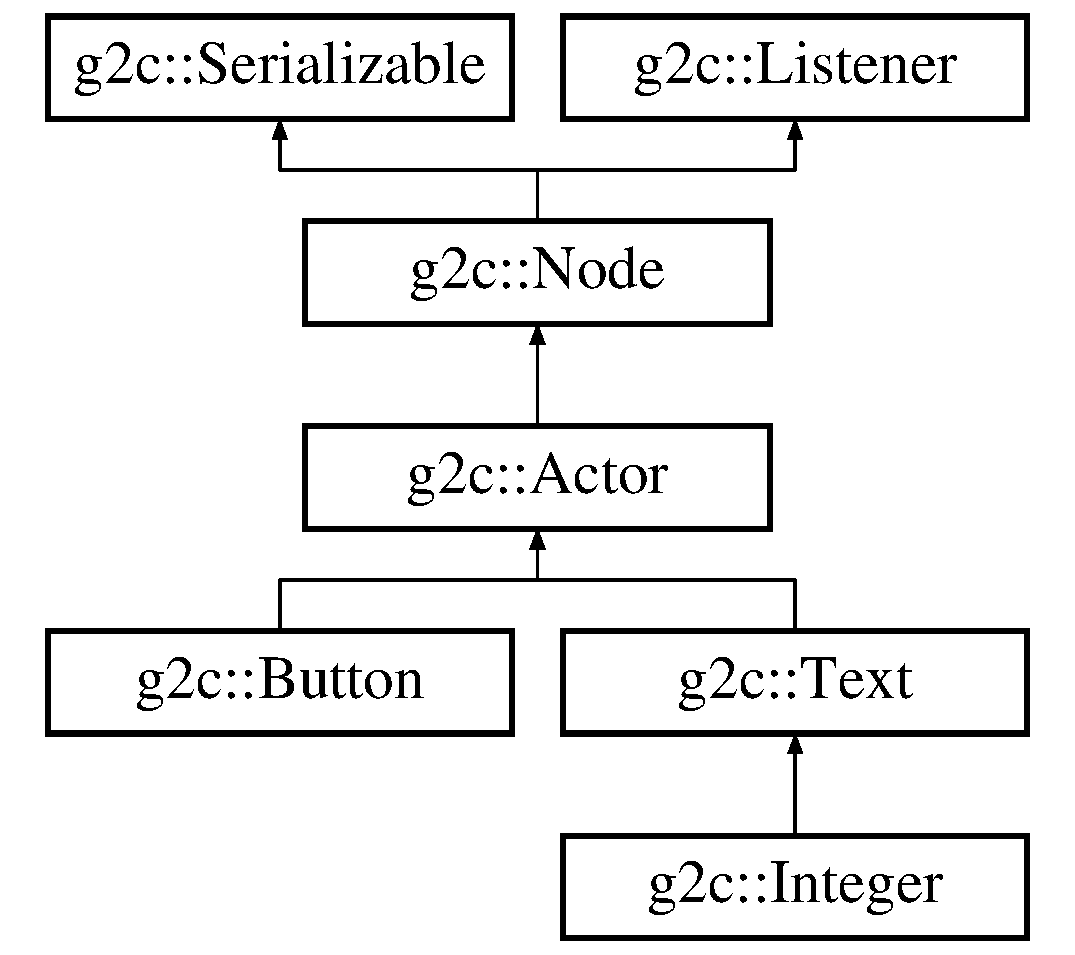
\includegraphics[height=5cm]{classg2c_1_1_actor}
\end{center}
\end{figure}
\subsection*{Public Member Functions}
\begin{DoxyCompactItemize}
\item 
\hyperlink{classg2c_1_1_actor_a1451aed47353957d0f8d74ee50c7104a}{Actor} (\hyperlink{classg2c_1_1_sprite}{Sprite} $\ast$insprite)
\item 
virtual void \hyperlink{classg2c_1_1_actor_a587aff8d8df73dbba0c659459e094074}{draw} () const 
\item 
\hypertarget{classg2c_1_1_actor_a42f0174a2b27e7c69d9a58911e210c06}{
virtual void {\bfseries handleChild} (const \hyperlink{classparse_1_1_node}{parse::Node} $\ast$n)}
\label{classg2c_1_1_actor_a42f0174a2b27e7c69d9a58911e210c06}

\item 
\hypertarget{classg2c_1_1_actor_adb5c4a33b015a9cf16a5d1076a479a0a}{
virtual \hyperlink{classg2c_1_1_polygon}{Polygon} {\bfseries collisionPolygon} () const }
\label{classg2c_1_1_actor_adb5c4a33b015a9cf16a5d1076a479a0a}

\item 
\hypertarget{classg2c_1_1_actor_a4c188103cf877e1cde49318ea9df493a}{
bool {\bfseries vectorInside} (const Vec2 \&C) const }
\label{classg2c_1_1_actor_a4c188103cf877e1cde49318ea9df493a}

\item 
\hypertarget{classg2c_1_1_actor_a699ccadcaf7be1db90aa5b7b5d94b6f3}{
virtual \hyperlink{classg2c_1_1_actor}{Actor} $\ast$ {\bfseries actorInClick} (const Vec2 \&C)}
\label{classg2c_1_1_actor_a699ccadcaf7be1db90aa5b7b5d94b6f3}

\item 
\hypertarget{classg2c_1_1_actor_acad54bfc77fe49491b32f01f3907535f}{
virtual void {\bfseries removeSprite} (const \hyperlink{classg2c_1_1_sprite}{Sprite} $\ast$sprite)}
\label{classg2c_1_1_actor_acad54bfc77fe49491b32f01f3907535f}

\end{DoxyCompactItemize}
\subsection*{Public Attributes}
\begin{DoxyCompactItemize}
\item 
\hypertarget{classg2c_1_1_actor_a8c539cd4fa278028f6c9db0e42027de6}{
\hyperlink{classg2c_1_1_sprite}{Sprite} $\ast$ {\bfseries sprite}}
\label{classg2c_1_1_actor_a8c539cd4fa278028f6c9db0e42027de6}

\item 
\hypertarget{classg2c_1_1_actor_a081ed2c7b4394e3c44284887ce9242d3}{
\hyperlink{classg2c_1_1_mesh}{Mesh} $\ast$ {\bfseries mesh}}
\label{classg2c_1_1_actor_a081ed2c7b4394e3c44284887ce9242d3}

\item 
double \& \hyperlink{classg2c_1_1_actor_aebf317d39fb7bf28c061741bd927f81f}{x}
\item 
double \& \hyperlink{classg2c_1_1_actor_ae627fd6cc00197b7e0a0b05d1d93b350}{y}
\item 
\hyperlink{classg2c_1_1_double_property}{DoubleProperty} \hyperlink{classg2c_1_1_actor_ab180e437af1643b93944397b5c1bc02f}{k}
\item 
\hyperlink{classg2c_1_1_int_property}{IntProperty} \hyperlink{classg2c_1_1_actor_a2b162d082f8f5e60463a4da42e9c58fd}{frame}
\item 
\hyperlink{classg2c_1_1_vec2_property}{Vec2Property} \hyperlink{classg2c_1_1_actor_aa674ee18247cbd0c2b908beb8496b71f}{position}
\item 
\hypertarget{classg2c_1_1_actor_a54a2f290b3e7ac35c98f170b961a9a4f}{
\hyperlink{classg2c_1_1_polygon}{Polygon} {\bfseries polygon}}
\label{classg2c_1_1_actor_a54a2f290b3e7ac35c98f170b961a9a4f}

\end{DoxyCompactItemize}


\subsection{Detailed Description}
An \hyperlink{classg2c_1_1_actor}{Actor} represents 2D graphics on the screen, typically a sprite at a particular 2D location with a current frame of animation. Several actors might use the same \hyperlink{classg2c_1_1_sprite}{Sprite}. For instance, a sprite might be a picture of a bullet, and a game with lots of bullets on the screen at the same time would use several Actors all pointing to the same \hyperlink{classg2c_1_1_sprite}{Sprite}.

An \hyperlink{classg2c_1_1_actor}{Actor} has a pointer to a \hyperlink{classg2c_1_1_sprite}{Sprite} and also a \hyperlink{classg2c_1_1_mesh}{Mesh}. \hyperlink{classg2c_1_1_actor_a587aff8d8df73dbba0c659459e094074}{Actor::draw()} draws the mesh using the sprite as a texture. If no \hyperlink{classg2c_1_1_mesh}{Mesh} is specified, a default rectangular mesh is used.

Actors can be positioned and scaled using x,y, and k, also a frame of animation that is current. The frame gets used to compute texture coordiates when drawing the mesh. 

\subsection{Constructor \& Destructor Documentation}
\hypertarget{classg2c_1_1_actor_a1451aed47353957d0f8d74ee50c7104a}{
\index{g2c::Actor@{g2c::Actor}!Actor@{Actor}}
\index{Actor@{Actor}!g2c::Actor@{g2c::Actor}}
\subsubsection[{Actor}]{\setlength{\rightskip}{0pt plus 5cm}g2c::Actor::Actor ({\bf Sprite} $\ast$ {\em insprite})\hspace{0.3cm}{\ttfamily  \mbox{[}explicit\mbox{]}}}}
\label{classg2c_1_1_actor_a1451aed47353957d0f8d74ee50c7104a}
Initializes the \hyperlink{classg2c_1_1_actor}{Actor} with given \hyperlink{classg2c_1_1_sprite}{Sprite} object. 

\subsection{Member Function Documentation}
\hypertarget{classg2c_1_1_actor_a587aff8d8df73dbba0c659459e094074}{
\index{g2c::Actor@{g2c::Actor}!draw@{draw}}
\index{draw@{draw}!g2c::Actor@{g2c::Actor}}
\subsubsection[{draw}]{\setlength{\rightskip}{0pt plus 5cm}void g2c::Actor::draw () const\hspace{0.3cm}{\ttfamily  \mbox{[}virtual\mbox{]}}}}
\label{classg2c_1_1_actor_a587aff8d8df73dbba0c659459e094074}
Draws mesh using sprite as a texture. If mesh is NULL, uses a default unit square \hyperlink{classg2c_1_1_mesh}{Mesh}. If sprite is NULL 

Reimplemented from \hyperlink{classg2c_1_1_node}{g2c::Node}.

Reimplemented in \hyperlink{classg2c_1_1_text_ab3296a30652c4c3157ae8a8e87449bb4}{g2c::Text}, \hyperlink{classg2c_1_1_integer_aac99d7502a55bf5db01f5d673779e36e}{g2c::Integer}, and \hyperlink{classg2c_1_1_button_a1d3bfdc06e37d9e533d1cd3b8d308579}{g2c::Button}.

\subsection{Member Data Documentation}
\hypertarget{classg2c_1_1_actor_a2b162d082f8f5e60463a4da42e9c58fd}{
\index{g2c::Actor@{g2c::Actor}!frame@{frame}}
\index{frame@{frame}!g2c::Actor@{g2c::Actor}}
\subsubsection[{frame}]{\setlength{\rightskip}{0pt plus 5cm}{\bf IntProperty} {\bf g2c::Actor::frame}}}
\label{classg2c_1_1_actor_a2b162d082f8f5e60463a4da42e9c58fd}
The index of the current frame of animation of the \hyperlink{classg2c_1_1_sprite}{Sprite} to draw. \hypertarget{classg2c_1_1_actor_ab180e437af1643b93944397b5c1bc02f}{
\index{g2c::Actor@{g2c::Actor}!k@{k}}
\index{k@{k}!g2c::Actor@{g2c::Actor}}
\subsubsection[{k}]{\setlength{\rightskip}{0pt plus 5cm}{\bf DoubleProperty} {\bf g2c::Actor::k}}}
\label{classg2c_1_1_actor_ab180e437af1643b93944397b5c1bc02f}
A scaling factor. \hypertarget{classg2c_1_1_actor_aa674ee18247cbd0c2b908beb8496b71f}{
\index{g2c::Actor@{g2c::Actor}!position@{position}}
\index{position@{position}!g2c::Actor@{g2c::Actor}}
\subsubsection[{position}]{\setlength{\rightskip}{0pt plus 5cm}{\bf Vec2Property} {\bf g2c::Actor::position}}}
\label{classg2c_1_1_actor_aa674ee18247cbd0c2b908beb8496b71f}
The 2D coordinates where to draw on the screen. \hypertarget{classg2c_1_1_actor_aebf317d39fb7bf28c061741bd927f81f}{
\index{g2c::Actor@{g2c::Actor}!x@{x}}
\index{x@{x}!g2c::Actor@{g2c::Actor}}
\subsubsection[{x}]{\setlength{\rightskip}{0pt plus 5cm}double\& {\bf g2c::Actor::x}}}
\label{classg2c_1_1_actor_aebf317d39fb7bf28c061741bd927f81f}
The x coordinate where to draw on the screen. Modifying x changes position. \hypertarget{classg2c_1_1_actor_ae627fd6cc00197b7e0a0b05d1d93b350}{
\index{g2c::Actor@{g2c::Actor}!y@{y}}
\index{y@{y}!g2c::Actor@{g2c::Actor}}
\subsubsection[{y}]{\setlength{\rightskip}{0pt plus 5cm}double\& {\bf g2c::Actor::y}}}
\label{classg2c_1_1_actor_ae627fd6cc00197b7e0a0b05d1d93b350}
The x coordinate where to draw on the screen. Modifying y changes position. 

The documentation for this class was generated from the following files:\begin{DoxyCompactItemize}
\item 
sprites.h\item 
sprites.cpp\end{DoxyCompactItemize}

\hypertarget{classg2c_1_1_android_bank}{
\section{g2c::AndroidBank Class Reference}
\label{classg2c_1_1_android_bank}\index{g2c::AndroidBank@{g2c::AndroidBank}}
}
Inheritance diagram for g2c::AndroidBank::\begin{figure}[H]
\begin{center}
\leavevmode
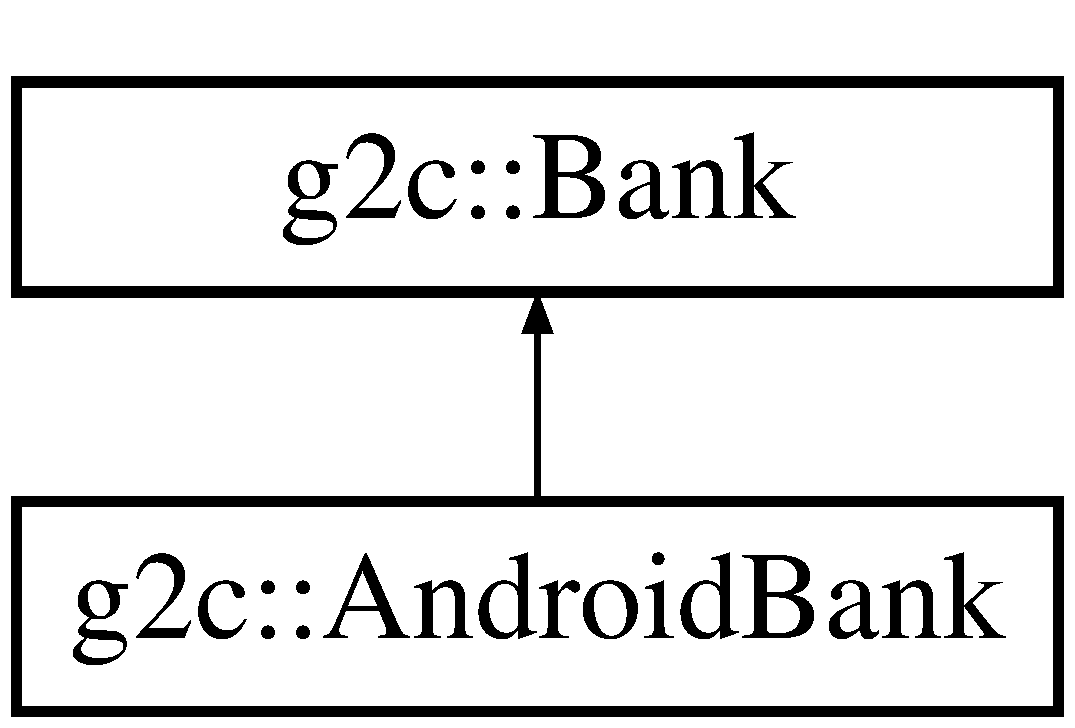
\includegraphics[height=2cm]{classg2c_1_1_android_bank}
\end{center}
\end{figure}
\subsection*{Public Member Functions}
\begin{DoxyCompactItemize}
\item 
\hypertarget{classg2c_1_1_android_bank_aad85a368a02c958e38f76dcf299fe593}{
void {\bfseries setEnvAndLoader} (JNIEnv $\ast$env, jobject loader)}
\label{classg2c_1_1_android_bank_aad85a368a02c958e38f76dcf299fe593}

\item 
\hypertarget{classg2c_1_1_android_bank_a98167dbfc1a6f50bbab5fde5c24a741d}{
virtual void {\bfseries initPersistentSerializableWithKey} (\hyperlink{classg2c_1_1_serializable}{Serializable} $\ast$s, const char $\ast$key)}
\label{classg2c_1_1_android_bank_a98167dbfc1a6f50bbab5fde5c24a741d}

\item 
\hypertarget{classg2c_1_1_android_bank_aedc069a046331b8047cd1161e2b3e097}{
virtual void {\bfseries writePersistentSerializableWithKey} (const \hyperlink{classg2c_1_1_serializable}{Serializable} $\ast$s, const char $\ast$key)}
\label{classg2c_1_1_android_bank_aedc069a046331b8047cd1161e2b3e097}

\item 
\hypertarget{classg2c_1_1_android_bank_a18d70ba1a018c6c316264988e64585df}{
virtual void {\bfseries initDataWithPath} (\hyperlink{classg2c_1_1_data}{Data} $\ast$s, const char $\ast$path)}
\label{classg2c_1_1_android_bank_a18d70ba1a018c6c316264988e64585df}

\item 
\hypertarget{classg2c_1_1_android_bank_aa0a295f281e919633e2e57fea8ed0284}{
virtual void {\bfseries initSerializableWithPath} (\hyperlink{classg2c_1_1_serializable}{Serializable} $\ast$s, const char $\ast$path)}
\label{classg2c_1_1_android_bank_aa0a295f281e919633e2e57fea8ed0284}

\item 
\hypertarget{classg2c_1_1_android_bank_a465bc912a08c521daa9abc70acbf1d31}{
virtual void {\bfseries writeSerializableToPath} (const \hyperlink{classg2c_1_1_serializable}{Serializable} $\ast$s, const char $\ast$path)}
\label{classg2c_1_1_android_bank_a465bc912a08c521daa9abc70acbf1d31}

\item 
\hypertarget{classg2c_1_1_android_bank_a4c3ec519498c068bb19d508de50596ba}{
virtual void {\bfseries initTextureWithPath} (\hyperlink{classg2c_1_1_texture2_d}{Texture2D} $\ast$texture, const char $\ast$path)}
\label{classg2c_1_1_android_bank_a4c3ec519498c068bb19d508de50596ba}

\item 
\hypertarget{classg2c_1_1_android_bank_ad8ed7533d1972b303a28b08a16cb80d4}{
virtual void {\bfseries initBitmapWithPath} (\hyperlink{classg2c_1_1_bitmap}{Bitmap} $\ast$bitmap, const char $\ast$path)}
\label{classg2c_1_1_android_bank_ad8ed7533d1972b303a28b08a16cb80d4}

\item 
\hypertarget{classg2c_1_1_android_bank_ac24ccb53727f30900e54015b998a4193}{
virtual void {\bfseries initSoundWithPath} (\hyperlink{classg2c_1_1_sound}{Sound} $\ast$sound, const char $\ast$path)}
\label{classg2c_1_1_android_bank_ac24ccb53727f30900e54015b998a4193}

\end{DoxyCompactItemize}
\subsection*{Public Attributes}
\begin{DoxyCompactItemize}
\item 
\hypertarget{classg2c_1_1_android_bank_a488d92aaa9c083f0d314c297dcf317b6}{
std::string {\bfseries base\_\-path}}
\label{classg2c_1_1_android_bank_a488d92aaa9c083f0d314c297dcf317b6}

\end{DoxyCompactItemize}
\subsection*{Protected Attributes}
\begin{DoxyCompactItemize}
\item 
\hypertarget{classg2c_1_1_android_bank_a27dcff59d476045db2ff67f46d9f276a}{
std::string {\bfseries directory}}
\label{classg2c_1_1_android_bank_a27dcff59d476045db2ff67f46d9f276a}

\item 
\hypertarget{classg2c_1_1_android_bank_afc2bf0d5b0d05401f44e27e4c320c134}{
JNIEnv $\ast$ {\bfseries env}}
\label{classg2c_1_1_android_bank_afc2bf0d5b0d05401f44e27e4c320c134}

\item 
\hypertarget{classg2c_1_1_android_bank_a6e90e2c21a7d6fb61836309c073fdca1}{
jobject {\bfseries loader}}
\label{classg2c_1_1_android_bank_a6e90e2c21a7d6fb61836309c073fdca1}

\end{DoxyCompactItemize}


The documentation for this class was generated from the following files:\begin{DoxyCompactItemize}
\item 
androidbank.h\item 
androidbank.cpp\end{DoxyCompactItemize}

\hypertarget{classg2c_1_1_animation}{
\section{g2c::Animation Class Reference}
\label{classg2c_1_1_animation}\index{g2c::Animation@{g2c::Animation}}
}
Inheritance diagram for g2c::Animation::\begin{figure}[H]
\begin{center}
\leavevmode
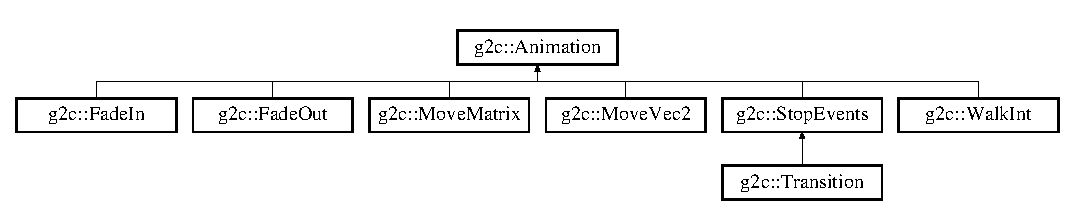
\includegraphics[height=2.45614cm]{classg2c_1_1_animation}
\end{center}
\end{figure}
\subsection*{Public Member Functions}
\begin{DoxyCompactItemize}
\item 
\hypertarget{classg2c_1_1_animation_a46ca60d97faa981cda59578cf1c5734c}{
{\bfseries Animation} (double instart)}
\label{classg2c_1_1_animation_a46ca60d97faa981cda59578cf1c5734c}

\item 
\hypertarget{classg2c_1_1_animation_a36e4196bfb5c1955ce750f884a741f43}{
{\bfseries Animation} (double instart, double induration)}
\label{classg2c_1_1_animation_a36e4196bfb5c1955ce750f884a741f43}

\item 
\hypertarget{classg2c_1_1_animation_a73d21f972a7c1f5af536d827fad8d3a8}{
virtual void {\bfseries advance} (double t)}
\label{classg2c_1_1_animation_a73d21f972a7c1f5af536d827fad8d3a8}

\item 
\hypertarget{classg2c_1_1_animation_aa271ceea2dbdb48b9a7ae43353c20cd6}{
virtual void {\bfseries begin} ()}
\label{classg2c_1_1_animation_aa271ceea2dbdb48b9a7ae43353c20cd6}

\item 
\hypertarget{classg2c_1_1_animation_ad05117579bf2e2d3d0c698c0b4b8596b}{
virtual void {\bfseries step} (double t)}
\label{classg2c_1_1_animation_ad05117579bf2e2d3d0c698c0b4b8596b}

\item 
\hypertarget{classg2c_1_1_animation_a53c2192f9b61c2d01c0651e0c239a68e}{
virtual void {\bfseries end} ()}
\label{classg2c_1_1_animation_a53c2192f9b61c2d01c0651e0c239a68e}

\item 
\hypertarget{classg2c_1_1_animation_a6e2f9faea125f0e604d374002a46e5d4}{
void {\bfseries print} () const }
\label{classg2c_1_1_animation_a6e2f9faea125f0e604d374002a46e5d4}

\item 
\hypertarget{classg2c_1_1_animation_ad4ae05fdbb106c726055109baf8c55ad}{
void {\bfseries display} () const }
\label{classg2c_1_1_animation_ad4ae05fdbb106c726055109baf8c55ad}

\end{DoxyCompactItemize}
\subsection*{Public Attributes}
\begin{DoxyCompactItemize}
\item 
\hypertarget{classg2c_1_1_animation_a20456d5d6aaefb4269661ab75475d48f}{
bool {\bfseries stopsEvents}}
\label{classg2c_1_1_animation_a20456d5d6aaefb4269661ab75475d48f}

\item 
\hypertarget{classg2c_1_1_animation_ae31ea2ad940df528e825ab11e9aa7398}{
bool {\bfseries forever}}
\label{classg2c_1_1_animation_ae31ea2ad940df528e825ab11e9aa7398}

\item 
\hypertarget{classg2c_1_1_animation_a84cfa640fd167aa91352787d10b4542e}{
bool {\bfseries running}}
\label{classg2c_1_1_animation_a84cfa640fd167aa91352787d10b4542e}

\item 
\hypertarget{classg2c_1_1_animation_a67aeb7b956f81a36d2f0d0d99034fdfe}{
double {\bfseries last}}
\label{classg2c_1_1_animation_a67aeb7b956f81a36d2f0d0d99034fdfe}

\item 
\hypertarget{classg2c_1_1_animation_a61b12f0405fbf1891c4c3e0fb14f2657}{
double {\bfseries start}}
\label{classg2c_1_1_animation_a61b12f0405fbf1891c4c3e0fb14f2657}

\item 
\hypertarget{classg2c_1_1_animation_a5c932c7485a503f9d261633ab11c211a}{
double {\bfseries duration}}
\label{classg2c_1_1_animation_a5c932c7485a503f9d261633ab11c211a}

\end{DoxyCompactItemize}
\subsection*{Friends}
\begin{DoxyCompactItemize}
\item 
\hypertarget{classg2c_1_1_animation_abbbfe7b916ef7239a2e95fdb21d0211f}{
class {\bfseries Animator}}
\label{classg2c_1_1_animation_abbbfe7b916ef7239a2e95fdb21d0211f}

\end{DoxyCompactItemize}


The documentation for this class was generated from the following files:\begin{DoxyCompactItemize}
\item 
sprites.h\item 
sprites.cpp\end{DoxyCompactItemize}

\hypertarget{classg2c_1_1_animator}{
\section{g2c::Animator Class Reference}
\label{classg2c_1_1_animator}\index{g2c::Animator@{g2c::Animator}}
}
\subsection*{Public Member Functions}
\begin{DoxyCompactItemize}
\item 
\hypertarget{classg2c_1_1_animator_ac51dc93cea31b2c20dcbfe7f6b0c896a}{
void {\bfseries add} (\hyperlink{classg2c_1_1_animation}{Animation} $\ast$)}
\label{classg2c_1_1_animator_ac51dc93cea31b2c20dcbfe7f6b0c896a}

\item 
\hypertarget{classg2c_1_1_animator_a471e7934efcc14c8fb0f8872a1390022}{
void {\bfseries remove} (\hyperlink{classg2c_1_1_animation}{Animation} $\ast$)}
\label{classg2c_1_1_animator_a471e7934efcc14c8fb0f8872a1390022}

\item 
\hypertarget{classg2c_1_1_animator_ac1b0e8adb7de9b8888824fc9ec182122}{
void {\bfseries retain} (\hyperlink{classg2c_1_1_animation}{Animation} $\ast$)}
\label{classg2c_1_1_animator_ac1b0e8adb7de9b8888824fc9ec182122}

\item 
\hypertarget{classg2c_1_1_animator_a9dd697653bcbd75597a35d613a5d7c05}{
bool {\bfseries release} (\hyperlink{classg2c_1_1_animation}{Animation} $\ast$)}
\label{classg2c_1_1_animator_a9dd697653bcbd75597a35d613a5d7c05}

\item 
\hypertarget{classg2c_1_1_animator_a9330fcd4fa0218eb37893af6899454e0}{
void {\bfseries step} (double t)}
\label{classg2c_1_1_animator_a9330fcd4fa0218eb37893af6899454e0}

\item 
\hypertarget{classg2c_1_1_animator_abae4565d93b82555c1f628cc4dc4df91}{
void {\bfseries clear} ()}
\label{classg2c_1_1_animator_abae4565d93b82555c1f628cc4dc4df91}

\end{DoxyCompactItemize}
\subsection*{Public Attributes}
\begin{DoxyCompactItemize}
\item 
\hypertarget{classg2c_1_1_animator_a6817e559374a8e57f8ac1ea596b64635}{
int {\bfseries eventStoppedCounter}}
\label{classg2c_1_1_animator_a6817e559374a8e57f8ac1ea596b64635}

\item 
\hypertarget{classg2c_1_1_animator_a757a0d19c9bb33da9d98dcd03b2a1663}{
std::set$<$ \hyperlink{classg2c_1_1_animation}{Animation} $\ast$ $>$ {\bfseries S}}
\label{classg2c_1_1_animator_a757a0d19c9bb33da9d98dcd03b2a1663}

\item 
\hypertarget{classg2c_1_1_animator_a0c6cfbc8f6b3a140e1fd101aa07f6cd1}{
std::vector$<$ \hyperlink{classg2c_1_1_listener}{Listener} $\ast$ $>$ {\bfseries listeners}}
\label{classg2c_1_1_animator_a0c6cfbc8f6b3a140e1fd101aa07f6cd1}

\item 
\hypertarget{classg2c_1_1_animator_a805f33797ca9074e59459bdd4486c42e}{
int {\bfseries animationsAdded}}
\label{classg2c_1_1_animator_a805f33797ca9074e59459bdd4486c42e}

\item 
\hypertarget{classg2c_1_1_animator_ae8d947257c92508cbdb189ecb33cd33a}{
int {\bfseries animationsRemoved}}
\label{classg2c_1_1_animator_ae8d947257c92508cbdb189ecb33cd33a}

\item 
\hypertarget{classg2c_1_1_animator_ad4fe0a77478d0ac8a0b129497b8f7e99}{
int {\bfseries animationsRemovedNotInList}}
\label{classg2c_1_1_animator_ad4fe0a77478d0ac8a0b129497b8f7e99}

\end{DoxyCompactItemize}


The documentation for this class was generated from the following files:\begin{DoxyCompactItemize}
\item 
sprites.h\item 
sprites.cpp\end{DoxyCompactItemize}

\hypertarget{classg2c_1_1_app}{
\section{g2c::App Class Reference}
\label{classg2c_1_1_app}\index{g2c::App@{g2c::App}}
}
\subsection*{Public Member Functions}
\begin{DoxyCompactItemize}
\item 
\hypertarget{classg2c_1_1_app_a7d948c9ba0a36f466a485f89a4990895}{
virtual void {\bfseries init} ()}
\label{classg2c_1_1_app_a7d948c9ba0a36f466a485f89a4990895}

\item 
\hypertarget{classg2c_1_1_app_aad38e92abc07652b16e28fc653727dcc}{
virtual void {\bfseries step} (double t)}
\label{classg2c_1_1_app_aad38e92abc07652b16e28fc653727dcc}

\item 
\hypertarget{classg2c_1_1_app_aafb3b402749a0cd10c1bf39e4c6ad7cf}{
virtual void {\bfseries draw} () const }
\label{classg2c_1_1_app_aafb3b402749a0cd10c1bf39e4c6ad7cf}

\item 
\hypertarget{classg2c_1_1_app_a4b9c3503ef383953559db5c8b03c4777}{
virtual bool {\bfseries mouseDown} (const Vec2 \&C)}
\label{classg2c_1_1_app_a4b9c3503ef383953559db5c8b03c4777}

\item 
\hypertarget{classg2c_1_1_app_a0e751be168e01f061a2161a0ac00e13a}{
virtual void {\bfseries mouseDragged} (const Vec2 \&C)}
\label{classg2c_1_1_app_a0e751be168e01f061a2161a0ac00e13a}

\item 
\hypertarget{classg2c_1_1_app_ae2580f73dab32b25e92f484096fdd888}{
virtual void {\bfseries mouseUp} (const Vec2 \&C)}
\label{classg2c_1_1_app_ae2580f73dab32b25e92f484096fdd888}

\item 
\hypertarget{classg2c_1_1_app_a4063add9296a5eadb6185d0f07c725d8}{
virtual bool {\bfseries touchDown} (unsigned int index, const Vec2 \&C)}
\label{classg2c_1_1_app_a4063add9296a5eadb6185d0f07c725d8}

\item 
\hypertarget{classg2c_1_1_app_a35026c076d87c5984a2ba443255ae65f}{
virtual void {\bfseries touchDragged} (unsigned int index, const Vec2 \&C)}
\label{classg2c_1_1_app_a35026c076d87c5984a2ba443255ae65f}

\item 
\hypertarget{classg2c_1_1_app_a596c05fe3c5926e500627f17c73746d0}{
virtual void {\bfseries touchUp} (unsigned int index, const Vec2 \&C)}
\label{classg2c_1_1_app_a596c05fe3c5926e500627f17c73746d0}

\item 
\hypertarget{classg2c_1_1_app_a340468d5d76774c57c0082b1ed7e5cba}{
virtual void {\bfseries keyboard} (unsigned char inkey)}
\label{classg2c_1_1_app_a340468d5d76774c57c0082b1ed7e5cba}

\item 
\hypertarget{classg2c_1_1_app_a7245a4bf6270cadd8238fa03436a43fb}{
virtual void {\bfseries special} (int inkey)}
\label{classg2c_1_1_app_a7245a4bf6270cadd8238fa03436a43fb}

\item 
\hypertarget{classg2c_1_1_app_aa7406471675bf5a0a1204f860b0147ea}{
virtual void {\bfseries reshape} (int width, int height)}
\label{classg2c_1_1_app_aa7406471675bf5a0a1204f860b0147ea}

\end{DoxyCompactItemize}


The documentation for this class was generated from the following files:\begin{DoxyCompactItemize}
\item 
app.h\item 
app.cpp\end{DoxyCompactItemize}

\hypertarget{classg2c_1_1_assumption}{
\section{g2c::Assumption Class Reference}
\label{classg2c_1_1_assumption}\index{g2c::Assumption@{g2c::Assumption}}
}
Inheritance diagram for g2c::Assumption::\begin{figure}[H]
\begin{center}
\leavevmode
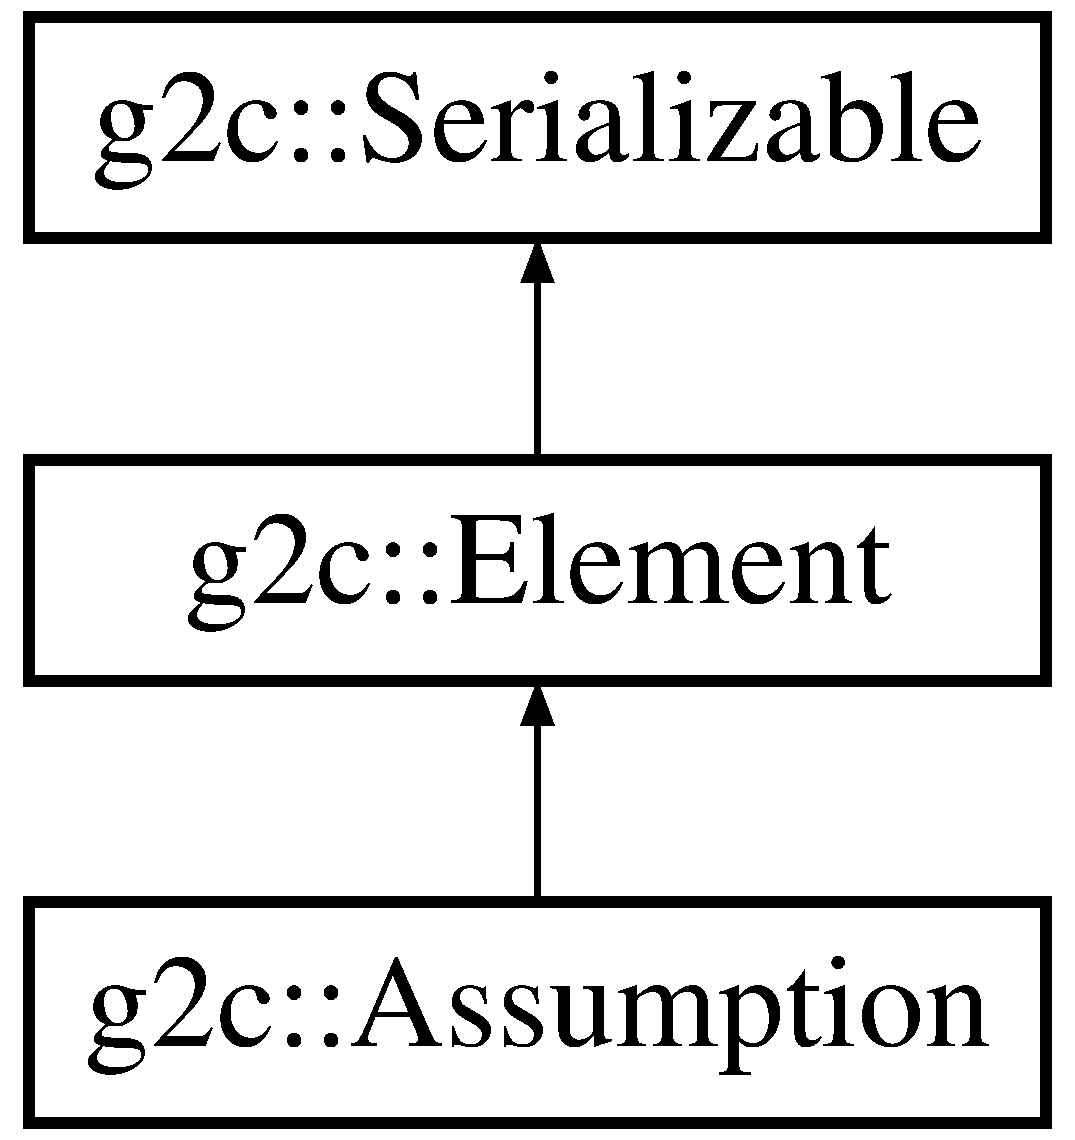
\includegraphics[height=3cm]{classg2c_1_1_assumption}
\end{center}
\end{figure}
\subsection*{Public Attributes}
\begin{DoxyCompactItemize}
\item 
\hypertarget{classg2c_1_1_assumption_aa5a89539db4258107c2fcbdc95b4ee74}{
bool {\bfseries active}}
\label{classg2c_1_1_assumption_aa5a89539db4258107c2fcbdc95b4ee74}

\item 
\hypertarget{classg2c_1_1_assumption_af09ecb4b149746a72cf7ab6917a6dcb0}{
std::string {\bfseries effectName}}
\label{classg2c_1_1_assumption_af09ecb4b149746a72cf7ab6917a6dcb0}

\item 
\hypertarget{classg2c_1_1_assumption_a951a0f8034a0f357b8d17ccd1344257b}{
\hyperlink{classg2c_1_1_effect}{Effect} $\ast$ {\bfseries effect}}
\label{classg2c_1_1_assumption_a951a0f8034a0f357b8d17ccd1344257b}

\end{DoxyCompactItemize}
\subsection*{Protected Member Functions}
\begin{DoxyCompactItemize}
\item 
\hypertarget{classg2c_1_1_assumption_ab001d47d3cfc825406359d282c538b66}{
virtual std::string {\bfseries serializeElements} (std::string indent=\char`\"{}\char`\"{}) const }
\label{classg2c_1_1_assumption_ab001d47d3cfc825406359d282c538b66}

\item 
\hypertarget{classg2c_1_1_assumption_af4c6aca5672389c5b95093b469e9f89c}{
virtual void {\bfseries handleChild} (const \hyperlink{classparse_1_1_node}{parse::Node} $\ast$n)}
\label{classg2c_1_1_assumption_af4c6aca5672389c5b95093b469e9f89c}

\end{DoxyCompactItemize}


The documentation for this class was generated from the following files:\begin{DoxyCompactItemize}
\item 
graphics.h\item 
graphics.cpp\end{DoxyCompactItemize}

\hypertarget{classg2c_1_1_asynchronous_bank}{
\section{g2c::AsynchronousBank Class Reference}
\label{classg2c_1_1_asynchronous_bank}\index{g2c::AsynchronousBank@{g2c::AsynchronousBank}}
}
Inheritance diagram for g2c::AsynchronousBank::\begin{figure}[H]
\begin{center}
\leavevmode
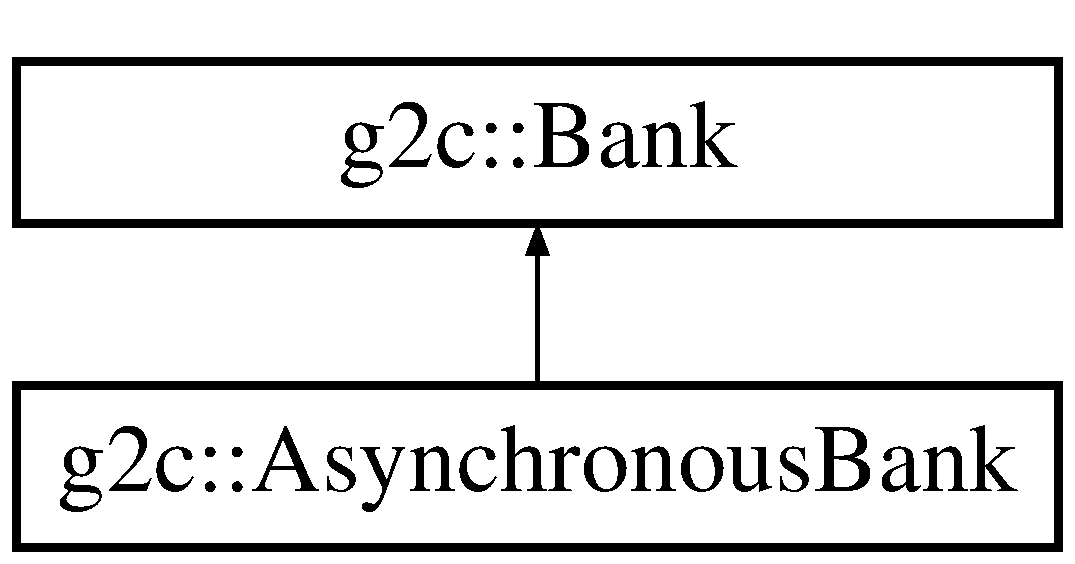
\includegraphics[height=2cm]{classg2c_1_1_asynchronous_bank}
\end{center}
\end{figure}
\subsection*{Classes}
\begin{DoxyCompactItemize}
\item 
struct \hyperlink{structg2c_1_1_asynchronous_bank_1_1_load_instruction}{LoadInstruction}
\end{DoxyCompactItemize}
\subsection*{Public Member Functions}
\begin{DoxyCompactItemize}
\item 
\hypertarget{classg2c_1_1_asynchronous_bank_afab7285f8e1791e41abd6616832efe01}{
virtual void {\bfseries initPersistentSerializableWithKey} (\hyperlink{classg2c_1_1_serializable}{Serializable} $\ast$s, const char $\ast$key)}
\label{classg2c_1_1_asynchronous_bank_afab7285f8e1791e41abd6616832efe01}

\item 
\hypertarget{classg2c_1_1_asynchronous_bank_ade98f9613a837c61a16ce801c8b8c8c3}{
virtual void {\bfseries writePersistentSerializableWithKey} (const \hyperlink{classg2c_1_1_serializable}{Serializable} $\ast$s, const char $\ast$key)}
\label{classg2c_1_1_asynchronous_bank_ade98f9613a837c61a16ce801c8b8c8c3}

\item 
\hypertarget{classg2c_1_1_asynchronous_bank_a45885d8428311718d15dbad91108192f}{
virtual void {\bfseries initSerializableWithPath} (\hyperlink{classg2c_1_1_serializable}{Serializable} $\ast$s, const char $\ast$path)}
\label{classg2c_1_1_asynchronous_bank_a45885d8428311718d15dbad91108192f}

\item 
\hypertarget{classg2c_1_1_asynchronous_bank_a671b5a907bd57ff8220af43d2abf79ac}{
virtual void {\bfseries writeSerializableToPath} (const \hyperlink{classg2c_1_1_serializable}{Serializable} $\ast$s, const char $\ast$path)}
\label{classg2c_1_1_asynchronous_bank_a671b5a907bd57ff8220af43d2abf79ac}

\item 
\hypertarget{classg2c_1_1_asynchronous_bank_ac0e1ec52f0bd4d38055bacb5e40bfece}{
virtual void {\bfseries initSoundWithPath} (\hyperlink{classg2c_1_1_sound}{Sound} $\ast$sound, const char $\ast$path)}
\label{classg2c_1_1_asynchronous_bank_ac0e1ec52f0bd4d38055bacb5e40bfece}

\item 
\hypertarget{classg2c_1_1_asynchronous_bank_ac7e1a291f4e9bb90d2579378c1519ead}{
virtual void {\bfseries initTextureWithPath} (\hyperlink{classg2c_1_1_texture2_d}{Texture2D} $\ast$texture, const char $\ast$path)}
\label{classg2c_1_1_asynchronous_bank_ac7e1a291f4e9bb90d2579378c1519ead}

\item 
\hypertarget{classg2c_1_1_asynchronous_bank_aa827f39fdf7e9cfd406cbb7c614d84a8}{
bool {\bfseries step} ()}
\label{classg2c_1_1_asynchronous_bank_aa827f39fdf7e9cfd406cbb7c614d84a8}

\item 
\hypertarget{classg2c_1_1_asynchronous_bank_ac010830c5098537586acd686caaa1f7c}{
int {\bfseries percent} () const }
\label{classg2c_1_1_asynchronous_bank_ac010830c5098537586acd686caaa1f7c}

\end{DoxyCompactItemize}
\subsection*{Public Attributes}
\begin{DoxyCompactItemize}
\item 
\hypertarget{classg2c_1_1_asynchronous_bank_a46a8b0cd639a460ca0d080dad41e4a97}{
\hyperlink{classg2c_1_1_bank}{Bank} $\ast$ {\bfseries bank}}
\label{classg2c_1_1_asynchronous_bank_a46a8b0cd639a460ca0d080dad41e4a97}

\end{DoxyCompactItemize}


The documentation for this class was generated from the following files:\begin{DoxyCompactItemize}
\item 
bank.h\item 
bank.cpp\end{DoxyCompactItemize}

\hypertarget{classg2c_1_1_bank}{
\section{g2c::Bank Class Reference}
\label{classg2c_1_1_bank}\index{g2c::Bank@{g2c::Bank}}
}
Inheritance diagram for g2c::Bank::\begin{figure}[H]
\begin{center}
\leavevmode
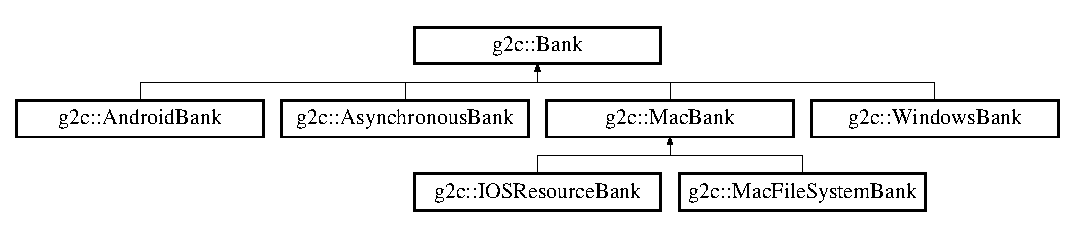
\includegraphics[height=2.6087cm]{classg2c_1_1_bank}
\end{center}
\end{figure}
\subsection*{Public Member Functions}
\begin{DoxyCompactItemize}
\item 
\hypertarget{classg2c_1_1_bank_aaa72c961f138d413dc8a8f94674def3f}{
virtual void {\bfseries initDataWithPath} (\hyperlink{classg2c_1_1_data}{Data} $\ast$data, const char $\ast$path)=0}
\label{classg2c_1_1_bank_aaa72c961f138d413dc8a8f94674def3f}

\item 
\hypertarget{classg2c_1_1_bank_a667198355eaab8b14e9eb3b74517e863}{
virtual void {\bfseries initPersistentSerializableWithKey} (\hyperlink{classg2c_1_1_serializable}{Serializable} $\ast$s, const char $\ast$key)=0}
\label{classg2c_1_1_bank_a667198355eaab8b14e9eb3b74517e863}

\item 
\hypertarget{classg2c_1_1_bank_a1d8081b137d998abd567d32405ec56b3}{
virtual void {\bfseries writePersistentSerializableWithKey} (const \hyperlink{classg2c_1_1_serializable}{Serializable} $\ast$s, const char $\ast$key)=0}
\label{classg2c_1_1_bank_a1d8081b137d998abd567d32405ec56b3}

\item 
\hypertarget{classg2c_1_1_bank_a40d817e1b28aa72c5e33b6a42c20c2a9}{
virtual void {\bfseries initSerializableWithPath} (\hyperlink{classg2c_1_1_serializable}{Serializable} $\ast$s, const char $\ast$path)=0}
\label{classg2c_1_1_bank_a40d817e1b28aa72c5e33b6a42c20c2a9}

\item 
\hypertarget{classg2c_1_1_bank_a66d420829fee68d113526e6d96cd1b3e}{
virtual void {\bfseries writeSerializableToPath} (const \hyperlink{classg2c_1_1_serializable}{Serializable} $\ast$s, const char $\ast$path)=0}
\label{classg2c_1_1_bank_a66d420829fee68d113526e6d96cd1b3e}

\item 
\hypertarget{classg2c_1_1_bank_abf6bf97f111007e22554275760805e21}{
virtual void {\bfseries initSoundWithPath} (\hyperlink{classg2c_1_1_sound}{Sound} $\ast$sound, const char $\ast$path)=0}
\label{classg2c_1_1_bank_abf6bf97f111007e22554275760805e21}

\item 
\hypertarget{classg2c_1_1_bank_abc03f2770abc1d5cc2f3a970fa01a6f3}{
virtual void {\bfseries initTextureWithPath} (\hyperlink{classg2c_1_1_texture2_d}{Texture2D} $\ast$texture, const char $\ast$path)=0}
\label{classg2c_1_1_bank_abc03f2770abc1d5cc2f3a970fa01a6f3}

\item 
\hypertarget{classg2c_1_1_bank_adeb9a83097a213f4fa90026e46197847}{
virtual void {\bfseries initBitmapWithPath} (\hyperlink{classg2c_1_1_bitmap}{Bitmap} $\ast$bitmap, const char $\ast$path)=0}
\label{classg2c_1_1_bank_adeb9a83097a213f4fa90026e46197847}

\end{DoxyCompactItemize}


The documentation for this class was generated from the following file:\begin{DoxyCompactItemize}
\item 
bank.h\end{DoxyCompactItemize}

\hypertarget{classg2c_1_1_bitmap}{
\section{g2c::Bitmap Class Reference}
\label{classg2c_1_1_bitmap}\index{g2c::Bitmap@{g2c::Bitmap}}
}
\subsection*{Public Member Functions}
\begin{DoxyCompactItemize}
\item 
\hypertarget{classg2c_1_1_bitmap_a8edd9cbb2dd99fa8ec2d7ded1a5718ee}{
{\bfseries Bitmap} (const \hyperlink{classg2c_1_1_bitmap}{Bitmap} \&b)}
\label{classg2c_1_1_bitmap_a8edd9cbb2dd99fa8ec2d7ded1a5718ee}

\item 
\hypertarget{classg2c_1_1_bitmap_a3b7f1edc2a3cd9bd3dcf68804bbff4d0}{
\hyperlink{classg2c_1_1_bitmap}{Bitmap} \& {\bfseries operator=} (const \hyperlink{classg2c_1_1_bitmap}{Bitmap} \&b)}
\label{classg2c_1_1_bitmap_a3b7f1edc2a3cd9bd3dcf68804bbff4d0}

\item 
\hypertarget{classg2c_1_1_bitmap_aef6fb7178471500e97e2dd245e41ffe1}{
void {\bfseries set} (uint8\_\-t $\ast$inData, int inWidth, int inHeight, int inBitsPerPixel)}
\label{classg2c_1_1_bitmap_aef6fb7178471500e97e2dd245e41ffe1}

\item 
\hypertarget{classg2c_1_1_bitmap_a73e7df56fa893320c8cc01a6d2fcca02}{
void {\bfseries flipVertically} ()}
\label{classg2c_1_1_bitmap_a73e7df56fa893320c8cc01a6d2fcca02}

\item 
\hypertarget{classg2c_1_1_bitmap_a1fdc123e65643b93bfbe38f8e3ff3c3f}{
void {\bfseries swizzleRGB} ()}
\label{classg2c_1_1_bitmap_a1fdc123e65643b93bfbe38f8e3ff3c3f}

\item 
\hypertarget{classg2c_1_1_bitmap_a74b534c4709c94d4f5ed7600bc52b254}{
const uint8\_\-t $\ast$const {\bfseries getData} () const }
\label{classg2c_1_1_bitmap_a74b534c4709c94d4f5ed7600bc52b254}

\item 
\hypertarget{classg2c_1_1_bitmap_a91d0a9005ecb9d10014287c0af546a71}{
int {\bfseries getWidth} () const }
\label{classg2c_1_1_bitmap_a91d0a9005ecb9d10014287c0af546a71}

\item 
\hypertarget{classg2c_1_1_bitmap_a13d3a898544b15ac4bcea3e50d9e90d9}{
int {\bfseries getHeight} () const }
\label{classg2c_1_1_bitmap_a13d3a898544b15ac4bcea3e50d9e90d9}

\item 
\hypertarget{classg2c_1_1_bitmap_af4c8d434b9b64fd3446b4df1438600fe}{
int {\bfseries getBitsPerPixel} () const }
\label{classg2c_1_1_bitmap_af4c8d434b9b64fd3446b4df1438600fe}

\end{DoxyCompactItemize}


The documentation for this class was generated from the following files:\begin{DoxyCompactItemize}
\item 
texture.h\item 
texture.cpp\end{DoxyCompactItemize}

\hypertarget{classg2c_1_1_bool_property}{
\section{g2c::BoolProperty Class Reference}
\label{classg2c_1_1_bool_property}\index{g2c::BoolProperty@{g2c::BoolProperty}}
}
Inheritance diagram for g2c::BoolProperty::\begin{figure}[H]
\begin{center}
\leavevmode
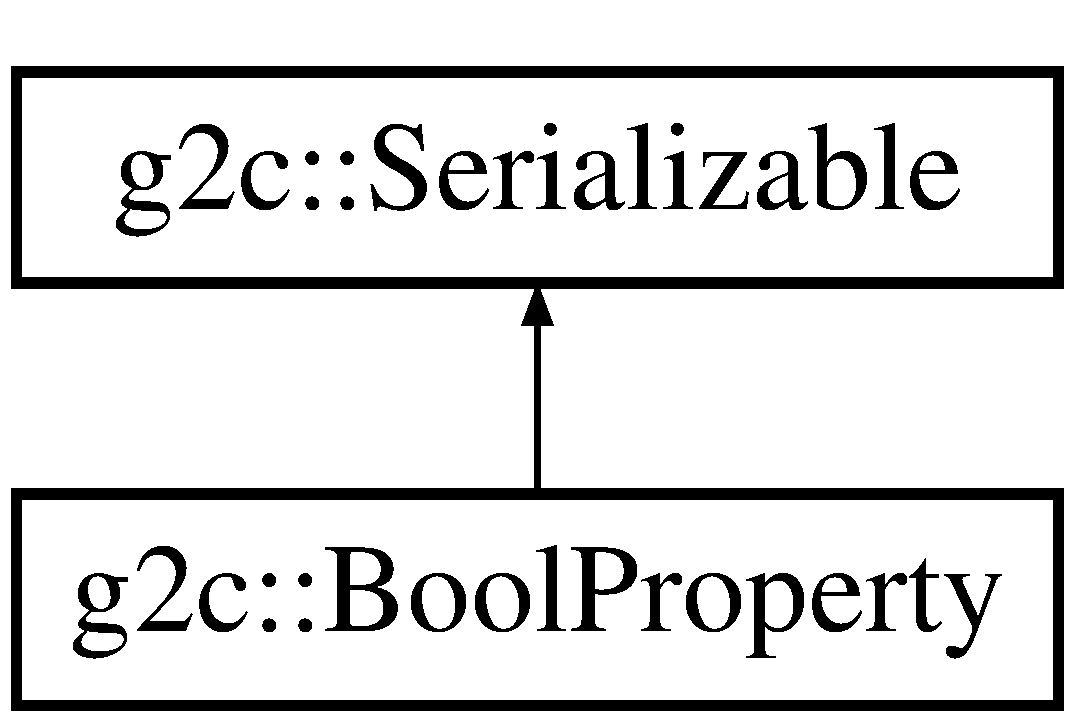
\includegraphics[height=2cm]{classg2c_1_1_bool_property}
\end{center}
\end{figure}
\subsection*{Public Member Functions}
\begin{DoxyCompactItemize}
\item 
\hypertarget{classg2c_1_1_bool_property_ac31860e2441f19d6acda9b54e85224db}{
{\bfseries BoolProperty} (bool b)}
\label{classg2c_1_1_bool_property_ac31860e2441f19d6acda9b54e85224db}

\item 
\hypertarget{classg2c_1_1_bool_property_a1325708460de1bd544f59c9043994fa0}{
virtual std::string {\bfseries serialize} (std::string indent=\char`\"{}\char`\"{}) const }
\label{classg2c_1_1_bool_property_a1325708460de1bd544f59c9043994fa0}

\item 
\hypertarget{classg2c_1_1_bool_property_a81028e4090ce23f59e8ea76e8512d1de}{
virtual void {\bfseries initWithParseNode} (const \hyperlink{classparse_1_1_node}{parse::Node} $\ast$n)}
\label{classg2c_1_1_bool_property_a81028e4090ce23f59e8ea76e8512d1de}

\item 
\hypertarget{classg2c_1_1_bool_property_a90c28add9250ea51adcc8fe85552c939}{
bool {\bfseries operator()} () const }
\label{classg2c_1_1_bool_property_a90c28add9250ea51adcc8fe85552c939}

\item 
\hypertarget{classg2c_1_1_bool_property_a3fca96a0b1a70b748e485e5c373760a3}{
void {\bfseries operator()} (bool b)}
\label{classg2c_1_1_bool_property_a3fca96a0b1a70b748e485e5c373760a3}

\item 
\hypertarget{classg2c_1_1_bool_property_af78c0cc4057b558b190af07272faa757}{
{\bfseries operator bool \&} ()}
\label{classg2c_1_1_bool_property_af78c0cc4057b558b190af07272faa757}

\item 
\hypertarget{classg2c_1_1_bool_property_a14bf6fd075588e8fa08c27c6bb171a61}{
{\bfseries operator bool} () const }
\label{classg2c_1_1_bool_property_a14bf6fd075588e8fa08c27c6bb171a61}

\end{DoxyCompactItemize}


The documentation for this class was generated from the following files:\begin{DoxyCompactItemize}
\item 
serializable.h\item 
serializable.cpp\end{DoxyCompactItemize}

\hypertarget{classg2c_1_1_buffer}{
\section{g2c::Buffer Class Reference}
\label{classg2c_1_1_buffer}\index{g2c::Buffer@{g2c::Buffer}}
}
Inheritance diagram for g2c::Buffer::\begin{figure}[H]
\begin{center}
\leavevmode
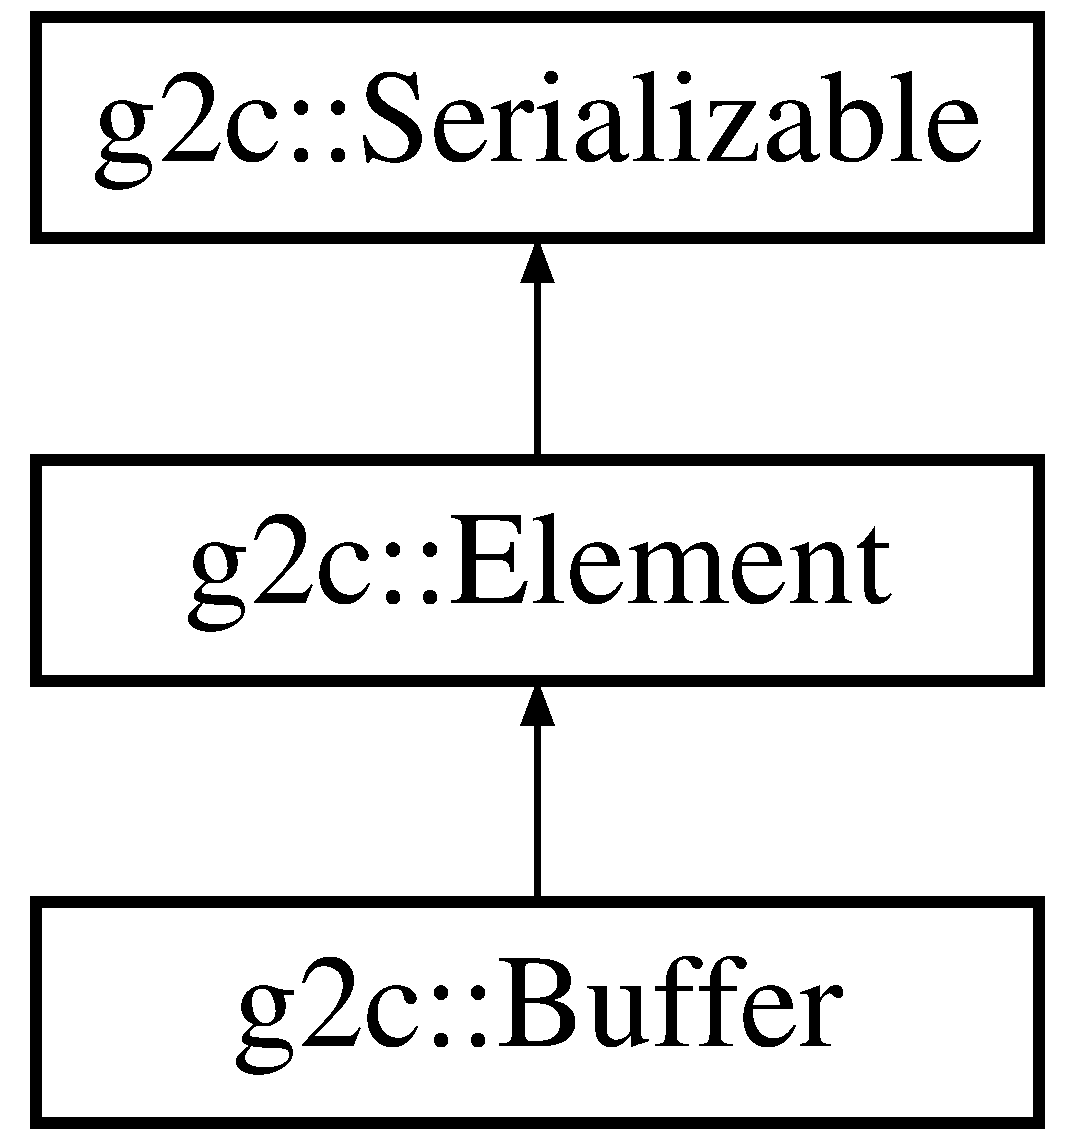
\includegraphics[height=3cm]{classg2c_1_1_buffer}
\end{center}
\end{figure}
\subsection*{Public Member Functions}
\begin{DoxyCompactItemize}
\item 
\hypertarget{classg2c_1_1_buffer_a768ab0f9efb6aeadad5ccf6a9433a3b4}{
{\bfseries Buffer} (const std::vector$<$ double $>$ \&v)}
\label{classg2c_1_1_buffer_a768ab0f9efb6aeadad5ccf6a9433a3b4}

\item 
\hypertarget{classg2c_1_1_buffer_a13f84ebc9ac0aa17b17d607aeb501b65}{
{\bfseries Buffer} (const std::vector$<$ float $>$ \&v)}
\label{classg2c_1_1_buffer_a13f84ebc9ac0aa17b17d607aeb501b65}

\item 
\hypertarget{classg2c_1_1_buffer_a0a56316bb76f1f208aec78ddbbca2e0e}{
{\bfseries Buffer} (const double $\ast$v, int size)}
\label{classg2c_1_1_buffer_a0a56316bb76f1f208aec78ddbbca2e0e}

\item 
\hypertarget{classg2c_1_1_buffer_a869186238b16b1fb3193a743808356bf}{
{\bfseries Buffer} (const float $\ast$v, int size)}
\label{classg2c_1_1_buffer_a869186238b16b1fb3193a743808356bf}

\end{DoxyCompactItemize}
\subsection*{Protected Member Functions}
\begin{DoxyCompactItemize}
\item 
\hypertarget{classg2c_1_1_buffer_ab8b7cf4a9712e88cba9b68408227720c}{
virtual std::string {\bfseries serializeElements} (std::string indent=\char`\"{}\char`\"{}) const }
\label{classg2c_1_1_buffer_ab8b7cf4a9712e88cba9b68408227720c}

\item 
\hypertarget{classg2c_1_1_buffer_a6452ddc818b9c692dbc817b5a2d6adac}{
virtual void {\bfseries handleChild} (const \hyperlink{classparse_1_1_node}{parse::Node} $\ast$n)}
\label{classg2c_1_1_buffer_a6452ddc818b9c692dbc817b5a2d6adac}

\end{DoxyCompactItemize}
\subsection*{Friends}
\begin{DoxyCompactItemize}
\item 
\hypertarget{classg2c_1_1_buffer_ac8649272bb0576cc72f2486439664efe}{
class {\bfseries Effect}}
\label{classg2c_1_1_buffer_ac8649272bb0576cc72f2486439664efe}

\end{DoxyCompactItemize}


The documentation for this class was generated from the following files:\begin{DoxyCompactItemize}
\item 
graphics.h\item 
graphics.cpp\end{DoxyCompactItemize}

\hypertarget{classg2c_1_1_button}{
\section{g2c::Button Class Reference}
\label{classg2c_1_1_button}\index{g2c::Button@{g2c::Button}}
}


{\ttfamily \#include $<$sprites.h$>$}Inheritance diagram for g2c::Button::\begin{figure}[H]
\begin{center}
\leavevmode
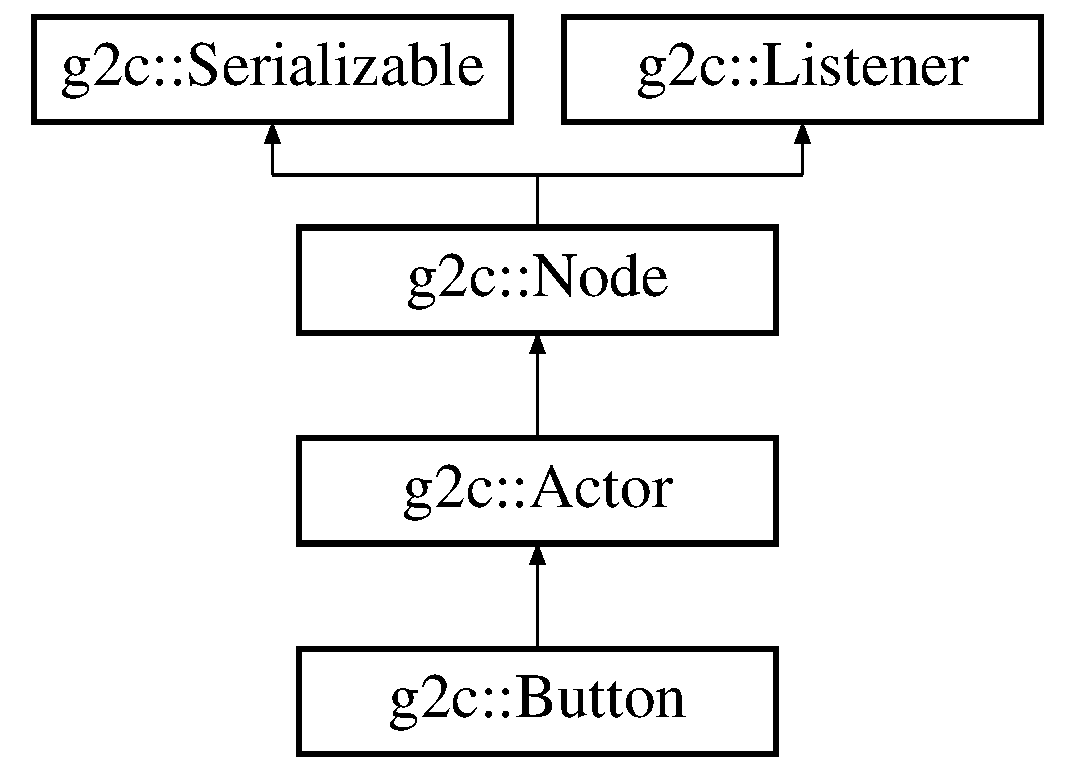
\includegraphics[height=4cm]{classg2c_1_1_button}
\end{center}
\end{figure}
\subsection*{Public Member Functions}
\begin{DoxyCompactItemize}
\item 
\hypertarget{classg2c_1_1_button_ac7275f502f751cde34c356e50f89e905}{
{\bfseries Button} (\hyperlink{classg2c_1_1_sprite}{Sprite} $\ast$insprite)}
\label{classg2c_1_1_button_ac7275f502f751cde34c356e50f89e905}

\item 
\hypertarget{classg2c_1_1_button_a8147322b847eb93b2b33157fed52cb54}{
{\bfseries Button} (\hyperlink{classg2c_1_1_sprite}{Sprite} $\ast$insprite, int inBaseFrame)}
\label{classg2c_1_1_button_a8147322b847eb93b2b33157fed52cb54}

\item 
virtual void \hyperlink{classg2c_1_1_button_a1d3bfdc06e37d9e533d1cd3b8d308579}{draw} () const 
\item 
\hypertarget{classg2c_1_1_button_a16bef8ab6b3469c521d280862349b9bb}{
virtual bool {\bfseries mouseDown} (const Vec2 \&C)}
\label{classg2c_1_1_button_a16bef8ab6b3469c521d280862349b9bb}

\item 
\hypertarget{classg2c_1_1_button_a6acf69a3fe5c60e1c8e496ec5978d16a}{
virtual void {\bfseries mouseDragged} (const Vec2 \&C)}
\label{classg2c_1_1_button_a6acf69a3fe5c60e1c8e496ec5978d16a}

\item 
\hypertarget{classg2c_1_1_button_adae476cd4698dd217c756d68f2efd168}{
virtual void {\bfseries mouseUp} (const Vec2 \&C)}
\label{classg2c_1_1_button_adae476cd4698dd217c756d68f2efd168}

\item 
\hypertarget{classg2c_1_1_button_a3c5e762a9c71aefd8b63a83554f5b4ad}{
virtual void {\bfseries handleChild} (const \hyperlink{classparse_1_1_node}{parse::Node} $\ast$n)}
\label{classg2c_1_1_button_a3c5e762a9c71aefd8b63a83554f5b4ad}

\item 
\hypertarget{classg2c_1_1_button_a7fa72e8406cbac161f0e349039f31089}{
std::string {\bfseries serializeElements} (std::string indent) const }
\label{classg2c_1_1_button_a7fa72e8406cbac161f0e349039f31089}

\end{DoxyCompactItemize}
\subsection*{Public Attributes}
\begin{DoxyCompactItemize}
\item 
\hypertarget{classg2c_1_1_button_a797aaa2f037cf86bdefe5995ae6f131d}{
int {\bfseries baseFrame}}
\label{classg2c_1_1_button_a797aaa2f037cf86bdefe5995ae6f131d}

\item 
\hypertarget{classg2c_1_1_button_ab94592bd21a7a9032e2d2ebed86d137f}{
bool {\bfseries depressed}}
\label{classg2c_1_1_button_ab94592bd21a7a9032e2d2ebed86d137f}

\item 
\hypertarget{classg2c_1_1_button_a6855cc7dd7780ffa232e3a8a542c71d0}{
\hyperlink{classg2c_1_1_button_handler}{ButtonHandler} $\ast$ {\bfseries handler}}
\label{classg2c_1_1_button_a6855cc7dd7780ffa232e3a8a542c71d0}

\end{DoxyCompactItemize}


\subsection{Detailed Description}
\hyperlink{classg2c_1_1_button}{Button} is a type of \hyperlink{classg2c_1_1_actor}{Actor} that is clickable, it is meant to draw as a sprite using a \hyperlink{classg2c_1_1_sprite}{Sprite} object just like its parent, except that it has its own implementations of mouseDown, mouseDragged and mouseUp which handle the animation of the button getting pushed.

To use a \hyperlink{classg2c_1_1_button}{Button}, instantiate one, set the button's sprite, set the integer baseFrame to the index of the frame of the sprite for the button in resting state. The next frame after that is assumed to be for the depressed state.

To implement a behaviour for the button when pressed, subclass \hyperlink{classg2c_1_1_button_handler}{ButtonHandler}, override click() function, and then set the button's handler element to an instance of that subclass. 

\subsection{Member Function Documentation}
\hypertarget{classg2c_1_1_button_a1d3bfdc06e37d9e533d1cd3b8d308579}{
\index{g2c::Button@{g2c::Button}!draw@{draw}}
\index{draw@{draw}!g2c::Button@{g2c::Button}}
\subsubsection[{draw}]{\setlength{\rightskip}{0pt plus 5cm}void g2c::Button::draw () const\hspace{0.3cm}{\ttfamily  \mbox{[}virtual\mbox{]}}}}
\label{classg2c_1_1_button_a1d3bfdc06e37d9e533d1cd3b8d308579}
Draws mesh using sprite as a texture. If mesh is NULL, uses a default unit square \hyperlink{classg2c_1_1_mesh}{Mesh}. If sprite is NULL 

Reimplemented from \hyperlink{classg2c_1_1_actor_a587aff8d8df73dbba0c659459e094074}{g2c::Actor}.

The documentation for this class was generated from the following files:\begin{DoxyCompactItemize}
\item 
sprites.h\item 
sprites.cpp\end{DoxyCompactItemize}

\hypertarget{classg2c_1_1_button_handler}{
\section{g2c::ButtonHandler Class Reference}
\label{classg2c_1_1_button_handler}\index{g2c::ButtonHandler@{g2c::ButtonHandler}}
}


{\ttfamily \#include $<$sprites.h$>$}\subsection*{Public Member Functions}
\begin{DoxyCompactItemize}
\item 
\hypertarget{classg2c_1_1_button_handler_adc10feaf556e7f9a1e27b45082e34e4e}{
virtual void {\bfseries down} (\hyperlink{classg2c_1_1_button}{Button} $\ast$button)}
\label{classg2c_1_1_button_handler_adc10feaf556e7f9a1e27b45082e34e4e}

\item 
\hypertarget{classg2c_1_1_button_handler_a28679b2bf70b70e75c4646c797374500}{
virtual void {\bfseries up} (\hyperlink{classg2c_1_1_button}{Button} $\ast$button)}
\label{classg2c_1_1_button_handler_a28679b2bf70b70e75c4646c797374500}

\item 
\hypertarget{classg2c_1_1_button_handler_ae42a49c45a666d4f16722c5e831cf968}{
virtual void {\bfseries click} (\hyperlink{classg2c_1_1_button}{Button} $\ast$button)=0}
\label{classg2c_1_1_button_handler_ae42a49c45a666d4f16722c5e831cf968}

\end{DoxyCompactItemize}


\subsection{Detailed Description}
Abstract helper class for \hyperlink{classg2c_1_1_button}{Button} the purpose of which is to hold the virtual function click(). Subclass \hyperlink{classg2c_1_1_button_handler}{ButtonHandler} and override click, then set a Button's handler element to an instnace of the subclass. click() will be called when the button is clicked. 

The documentation for this class was generated from the following files:\begin{DoxyCompactItemize}
\item 
sprites.h\item 
sprites.cpp\end{DoxyCompactItemize}

\hypertarget{classg2c_1_1_color}{
\section{g2c::Color Class Reference}
\label{classg2c_1_1_color}\index{g2c::Color@{g2c::Color}}
}
Inheritance diagram for g2c::Color::\begin{figure}[H]
\begin{center}
\leavevmode
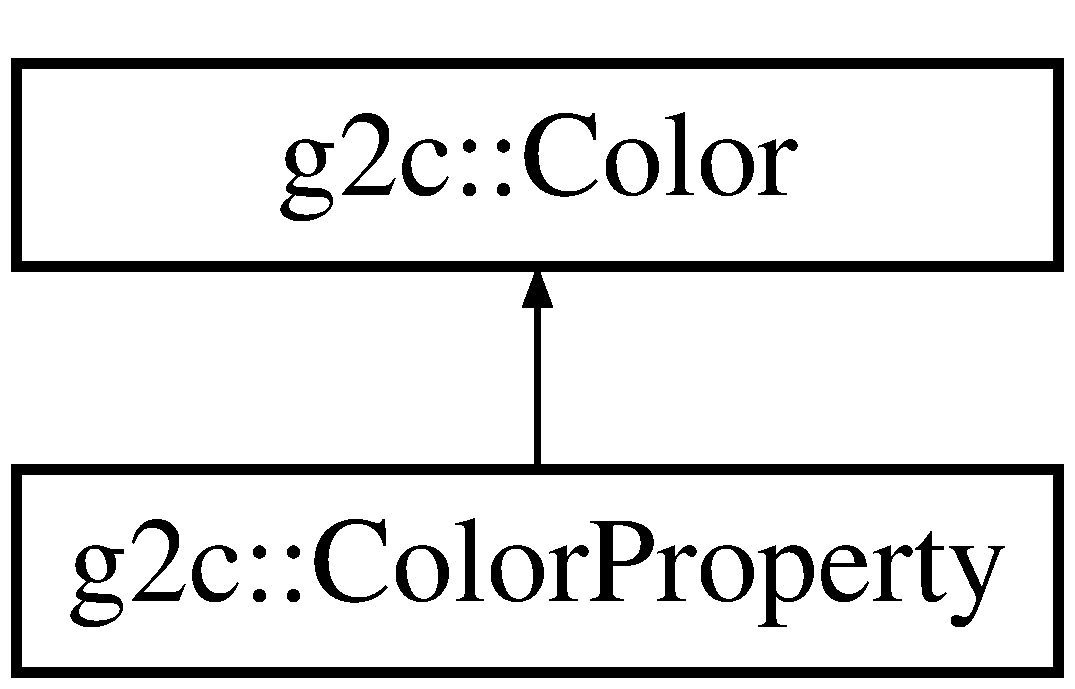
\includegraphics[height=2cm]{classg2c_1_1_color}
\end{center}
\end{figure}
\subsection*{Public Member Functions}
\begin{DoxyCompactItemize}
\item 
\hypertarget{classg2c_1_1_color_a6c42a25920b142136d2ee34fe3490e9d}{
{\bfseries Color} (double r, double g, double b, double a)}
\label{classg2c_1_1_color_a6c42a25920b142136d2ee34fe3490e9d}

\item 
\hypertarget{classg2c_1_1_color_a9f5ddd4f246e0d973f4258314a5f1073}{
{\bfseries Color} (const \hyperlink{classg2c_1_1_color}{Color} \&c)}
\label{classg2c_1_1_color_a9f5ddd4f246e0d973f4258314a5f1073}

\item 
\hypertarget{classg2c_1_1_color_aab192298aaf7306a2a96a89e302ca006}{
{\bfseries Color} (const Vec4 \&c)}
\label{classg2c_1_1_color_aab192298aaf7306a2a96a89e302ca006}

\item 
\hypertarget{classg2c_1_1_color_af28e509730f2efda299eb7f321a2e9fd}{
\hyperlink{classg2c_1_1_color}{Color} \& {\bfseries operator=} (const \hyperlink{classg2c_1_1_color}{Color} \&v)}
\label{classg2c_1_1_color_af28e509730f2efda299eb7f321a2e9fd}

\end{DoxyCompactItemize}
\subsection*{Public Attributes}
\begin{DoxyCompactItemize}
\item 
\hypertarget{classg2c_1_1_color_a220175ad46233fa38e95e29e0b835b51}{
double \& {\bfseries r}}
\label{classg2c_1_1_color_a220175ad46233fa38e95e29e0b835b51}

\item 
\hypertarget{classg2c_1_1_color_a9bd8336365fca3ec12ee4613ed2317e9}{
double \& {\bfseries g}}
\label{classg2c_1_1_color_a9bd8336365fca3ec12ee4613ed2317e9}

\item 
\hypertarget{classg2c_1_1_color_abed8ad7dc0dfe06fd35900df9e293073}{
double \& {\bfseries b}}
\label{classg2c_1_1_color_abed8ad7dc0dfe06fd35900df9e293073}

\item 
\hypertarget{classg2c_1_1_color_acfdf10b4267939d773d5f2a2d171b6ef}{
double \& {\bfseries a}}
\label{classg2c_1_1_color_acfdf10b4267939d773d5f2a2d171b6ef}

\end{DoxyCompactItemize}


The documentation for this class was generated from the following file:\begin{DoxyCompactItemize}
\item 
sprites.h\end{DoxyCompactItemize}

\hypertarget{classg2c_1_1_color_property}{
\section{g2c::ColorProperty Class Reference}
\label{classg2c_1_1_color_property}\index{g2c::ColorProperty@{g2c::ColorProperty}}
}
Inheritance diagram for g2c::ColorProperty::\begin{figure}[H]
\begin{center}
\leavevmode
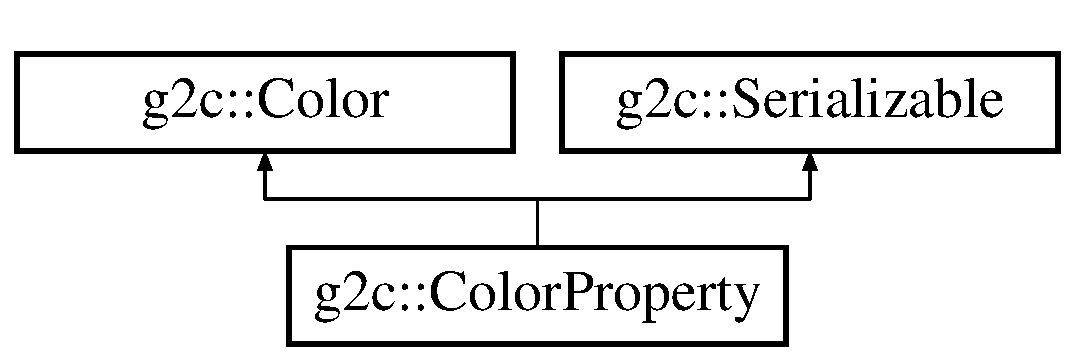
\includegraphics[height=2cm]{classg2c_1_1_color_property}
\end{center}
\end{figure}
\subsection*{Public Member Functions}
\begin{DoxyCompactItemize}
\item 
\hypertarget{classg2c_1_1_color_property_a0342ab7b0cb34333e74bf597fe18472d}{
{\bfseries ColorProperty} (const \hyperlink{classg2c_1_1_color}{Color} \&c)}
\label{classg2c_1_1_color_property_a0342ab7b0cb34333e74bf597fe18472d}

\item 
\hypertarget{classg2c_1_1_color_property_a17c8597e111e9d1da1d27d563312f220}{
\hyperlink{classg2c_1_1_color_property}{ColorProperty} \& {\bfseries operator=} (const \hyperlink{classg2c_1_1_color}{Color} \&v)}
\label{classg2c_1_1_color_property_a17c8597e111e9d1da1d27d563312f220}

\item 
\hypertarget{classg2c_1_1_color_property_aef34a6c20e5767e16d95f713013bd4a0}{
virtual std::string {\bfseries serialize} (std::string indent) const }
\label{classg2c_1_1_color_property_aef34a6c20e5767e16d95f713013bd4a0}

\item 
\hypertarget{classg2c_1_1_color_property_aeef6cc3b62b9ddca119280f3cccf7055}{
void {\bfseries initWithParseNode} (const \hyperlink{classparse_1_1_node}{parse::Node} $\ast$n)}
\label{classg2c_1_1_color_property_aeef6cc3b62b9ddca119280f3cccf7055}

\end{DoxyCompactItemize}


The documentation for this class was generated from the following files:\begin{DoxyCompactItemize}
\item 
sprites.h\item 
sprites.cpp\end{DoxyCompactItemize}

\hypertarget{classg2c_1_1_context}{
\section{g2c::Context Class Reference}
\label{classg2c_1_1_context}\index{g2c::Context@{g2c::Context}}
}
\subsection*{Public Member Functions}
\begin{DoxyCompactItemize}
\item 
\hypertarget{classg2c_1_1_context_ab8f6f307b7e213c10047faa3446d8b46}{
{\bfseries Context} (\hyperlink{classg2c_1_1_player}{Player} $\ast$player)}
\label{classg2c_1_1_context_ab8f6f307b7e213c10047faa3446d8b46}

\item 
\hypertarget{classg2c_1_1_context_ade254ad4d223f8d57aa0cfb3f2d61769}{
void {\bfseries makeCurrent} ()}
\label{classg2c_1_1_context_ade254ad4d223f8d57aa0cfb3f2d61769}

\end{DoxyCompactItemize}
\subsection*{Friends}
\begin{DoxyCompactItemize}
\item 
\hypertarget{classg2c_1_1_context_a50914f77c7cf4fb97616c898c5291f4b}{
class {\bfseries Sound}}
\label{classg2c_1_1_context_a50914f77c7cf4fb97616c898c5291f4b}

\item 
\hypertarget{classg2c_1_1_context_afec7d2c89abca6ba2f2278a4ec21fc00}{
class {\bfseries Source}}
\label{classg2c_1_1_context_afec7d2c89abca6ba2f2278a4ec21fc00}

\end{DoxyCompactItemize}


The documentation for this class was generated from the following files:\begin{DoxyCompactItemize}
\item 
sound.h\item 
sound.cpp\end{DoxyCompactItemize}

\hypertarget{classg2c_1_1_cube_map}{
\section{g2c::CubeMap Class Reference}
\label{classg2c_1_1_cube_map}\index{g2c::CubeMap@{g2c::CubeMap}}
}
Inheritance diagram for g2c::CubeMap::\begin{figure}[H]
\begin{center}
\leavevmode
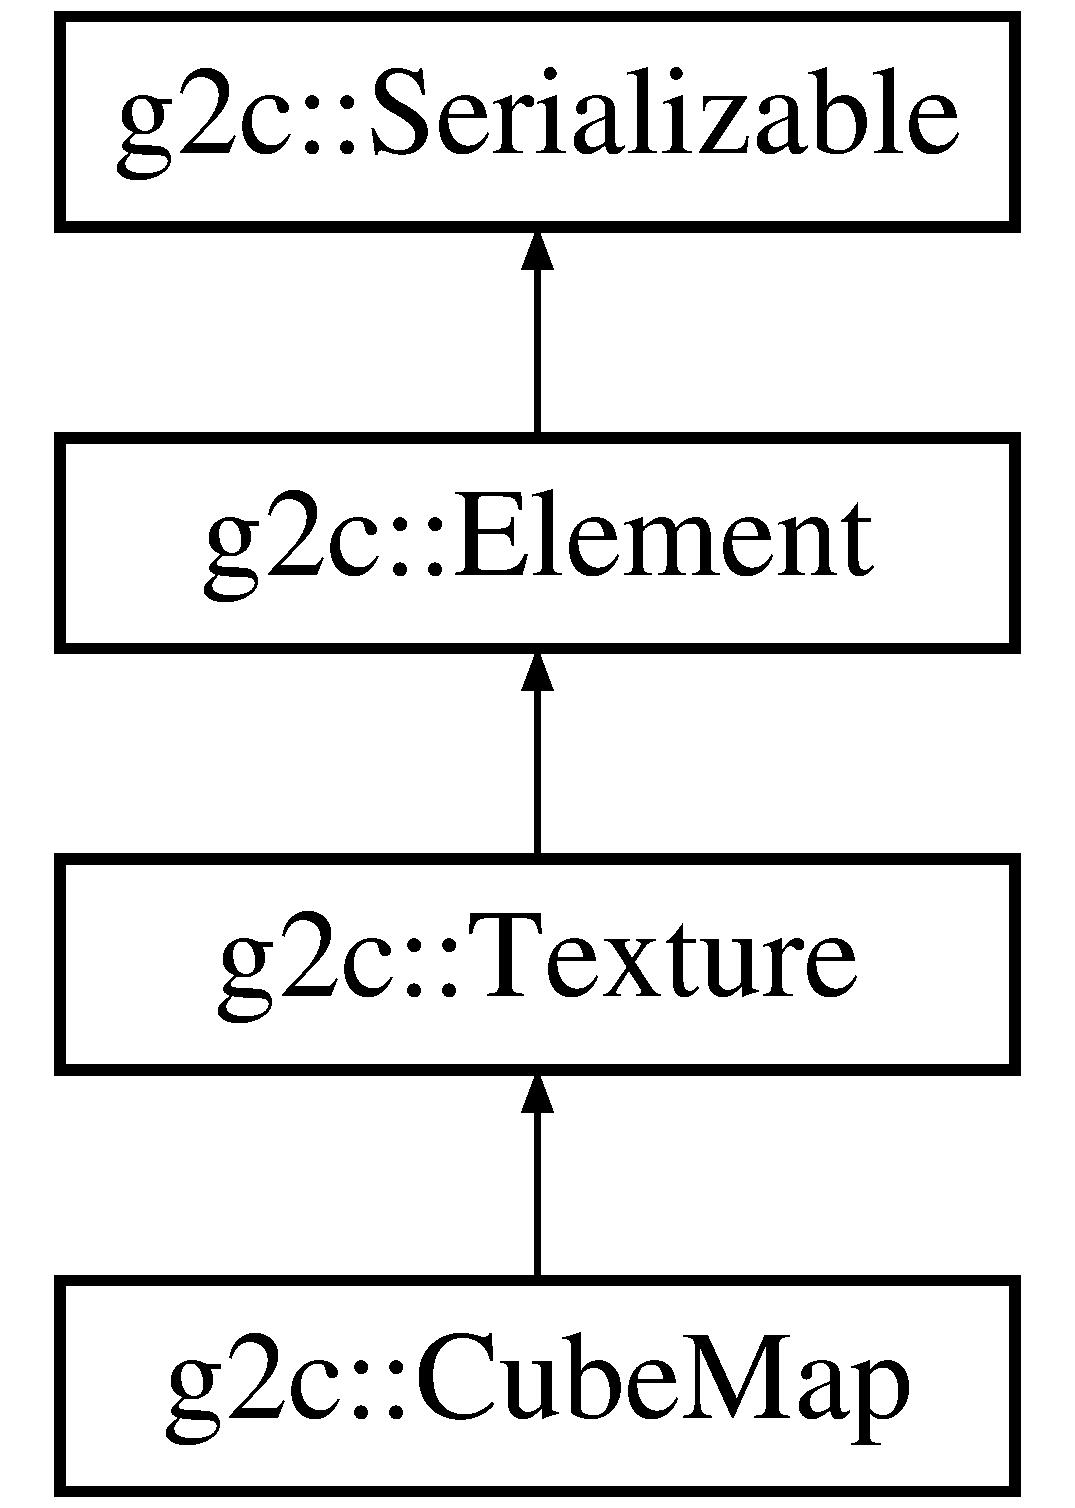
\includegraphics[height=4cm]{classg2c_1_1_cube_map}
\end{center}
\end{figure}
\subsection*{Public Member Functions}
\begin{DoxyCompactItemize}
\item 
\hypertarget{classg2c_1_1_cube_map_a8ccdab98236e6d1a25a352edc4b84c40}{
{\bfseries CubeMap} (int unit)}
\label{classg2c_1_1_cube_map_a8ccdab98236e6d1a25a352edc4b84c40}

\item 
\hypertarget{classg2c_1_1_cube_map_aaac886cf9fbbdd8baf37998017e9168a}{
void {\bfseries initWithImageData} (const GLubyte $\ast$positiveXData, const GLubyte $\ast$negativeXData, const GLubyte $\ast$positiveYData, const GLubyte $\ast$negativeYData, const GLubyte $\ast$positiveZData, const GLubyte $\ast$negativeZData, int inWidth, int inBitsPerPixel)}
\label{classg2c_1_1_cube_map_aaac886cf9fbbdd8baf37998017e9168a}

\item 
\hypertarget{classg2c_1_1_cube_map_ac771220017a469ab3cb5fb388f2d4c29}{
void {\bfseries initWithBitmaps} (const \hyperlink{classg2c_1_1_bitmap}{Bitmap} \&bitmapPositiveX, const \hyperlink{classg2c_1_1_bitmap}{Bitmap} \&bitmapNegativeX, const \hyperlink{classg2c_1_1_bitmap}{Bitmap} \&bitmapPositiveY, const \hyperlink{classg2c_1_1_bitmap}{Bitmap} \&bitmapNegativeY, const \hyperlink{classg2c_1_1_bitmap}{Bitmap} \&bitmapPositiveZ, const \hyperlink{classg2c_1_1_bitmap}{Bitmap} \&bitmapNegativeZ)}
\label{classg2c_1_1_cube_map_ac771220017a469ab3cb5fb388f2d4c29}

\end{DoxyCompactItemize}
\subsection*{Public Attributes}
\begin{DoxyCompactItemize}
\item 
\hypertarget{classg2c_1_1_cube_map_a25677e3926095e106b83e4406688bc9c}{
int {\bfseries width}}
\label{classg2c_1_1_cube_map_a25677e3926095e106b83e4406688bc9c}

\item 
\hypertarget{classg2c_1_1_cube_map_aa207f97d38424b66825bb447a71b0cec}{
std::string {\bfseries positiveXFile}}
\label{classg2c_1_1_cube_map_aa207f97d38424b66825bb447a71b0cec}

\item 
\hypertarget{classg2c_1_1_cube_map_a410eebe9ff923407e7793ec7357484e5}{
std::string {\bfseries negativeXFile}}
\label{classg2c_1_1_cube_map_a410eebe9ff923407e7793ec7357484e5}

\item 
\hypertarget{classg2c_1_1_cube_map_a3d134e8eb82816053111731676c57c45}{
std::string {\bfseries positiveYFile}}
\label{classg2c_1_1_cube_map_a3d134e8eb82816053111731676c57c45}

\item 
\hypertarget{classg2c_1_1_cube_map_ab6548ef34db04e1d1997592428ce7d6d}{
std::string {\bfseries negativeYFile}}
\label{classg2c_1_1_cube_map_ab6548ef34db04e1d1997592428ce7d6d}

\item 
\hypertarget{classg2c_1_1_cube_map_a5c2ce3f42e96695f6a75afe40563e1f2}{
std::string {\bfseries positiveZFile}}
\label{classg2c_1_1_cube_map_a5c2ce3f42e96695f6a75afe40563e1f2}

\item 
\hypertarget{classg2c_1_1_cube_map_a8651988d4b3c3a6bbb35dd428dabd57c}{
std::string {\bfseries negativeZFile}}
\label{classg2c_1_1_cube_map_a8651988d4b3c3a6bbb35dd428dabd57c}

\end{DoxyCompactItemize}
\subsection*{Protected Member Functions}
\begin{DoxyCompactItemize}
\item 
\hypertarget{classg2c_1_1_cube_map_a45fe1d91eaeb89ef171bb1cc06c69ca3}{
virtual std::string {\bfseries serializeElements} (std::string indent=\char`\"{}\char`\"{}) const }
\label{classg2c_1_1_cube_map_a45fe1d91eaeb89ef171bb1cc06c69ca3}

\item 
\hypertarget{classg2c_1_1_cube_map_a6ee20db7e6fc1de8ae52e7083b459b2b}{
virtual void {\bfseries handleChild} (const \hyperlink{classparse_1_1_node}{parse::Node} $\ast$n)}
\label{classg2c_1_1_cube_map_a6ee20db7e6fc1de8ae52e7083b459b2b}

\end{DoxyCompactItemize}
\subsection*{Friends}
\begin{DoxyCompactItemize}
\item 
\hypertarget{classg2c_1_1_cube_map_aeceedf6e1a7d48a588516ce2b1983d6f}{
class {\bfseries Value}}
\label{classg2c_1_1_cube_map_aeceedf6e1a7d48a588516ce2b1983d6f}

\end{DoxyCompactItemize}


The documentation for this class was generated from the following files:\begin{DoxyCompactItemize}
\item 
texture.h\item 
texture.cpp\end{DoxyCompactItemize}

\hypertarget{classg2c_1_1_data}{
\section{g2c::Data Class Reference}
\label{classg2c_1_1_data}\index{g2c::Data@{g2c::Data}}
}
\subsection*{Public Member Functions}
\begin{DoxyCompactItemize}
\item 
\hypertarget{classg2c_1_1_data_a31e0ba61d61c0b0d40a365b0f99013b1}{
uint8\_\-t $\ast$ {\bfseries array} () const }
\label{classg2c_1_1_data_a31e0ba61d61c0b0d40a365b0f99013b1}

\item 
\hypertarget{classg2c_1_1_data_a6c089a44150a66e120fd39d38897b030}{
size\_\-t {\bfseries size} () const }
\label{classg2c_1_1_data_a6c089a44150a66e120fd39d38897b030}

\item 
\hypertarget{classg2c_1_1_data_a74f277f71c65e18265892af281dc205f}{
void {\bfseries resize} (size\_\-t size)}
\label{classg2c_1_1_data_a74f277f71c65e18265892af281dc205f}

\end{DoxyCompactItemize}


The documentation for this class was generated from the following files:\begin{DoxyCompactItemize}
\item 
bank.h\item 
bank.cpp\end{DoxyCompactItemize}

\hypertarget{classparse_1_1_data}{
\section{parse::Data Class Reference}
\label{classparse_1_1_data}\index{parse::Data@{parse::Data}}
}
\subsection*{Public Attributes}
\begin{DoxyCompactItemize}
\item 
\hypertarget{classparse_1_1_data_a63cec840a32b4c34f9ae0435b61e30e0}{
int {\bfseries i}}
\label{classparse_1_1_data_a63cec840a32b4c34f9ae0435b61e30e0}

\item 
\hypertarget{classparse_1_1_data_af4a131eb71a7290bf07fb8d8cf6f3b25}{
double {\bfseries x}}
\label{classparse_1_1_data_af4a131eb71a7290bf07fb8d8cf6f3b25}

\item 
\hypertarget{classparse_1_1_data_aff5da6a946ede974df321c10537656a5}{
std::string {\bfseries s}}
\label{classparse_1_1_data_aff5da6a946ede974df321c10537656a5}

\item 
\hypertarget{classparse_1_1_data_a75d7093eefe47e1747f2dde884e78cf6}{
\hyperlink{classparse_1_1_node}{Node} $\ast$ {\bfseries value}}
\label{classparse_1_1_data_a75d7093eefe47e1747f2dde884e78cf6}

\end{DoxyCompactItemize}


The documentation for this class was generated from the following file:\begin{DoxyCompactItemize}
\item 
parse.h\end{DoxyCompactItemize}

\hypertarget{classg2c_1_1_double_property}{
\section{g2c::DoubleProperty Class Reference}
\label{classg2c_1_1_double_property}\index{g2c::DoubleProperty@{g2c::DoubleProperty}}
}
Inheritance diagram for g2c::DoubleProperty::\begin{figure}[H]
\begin{center}
\leavevmode
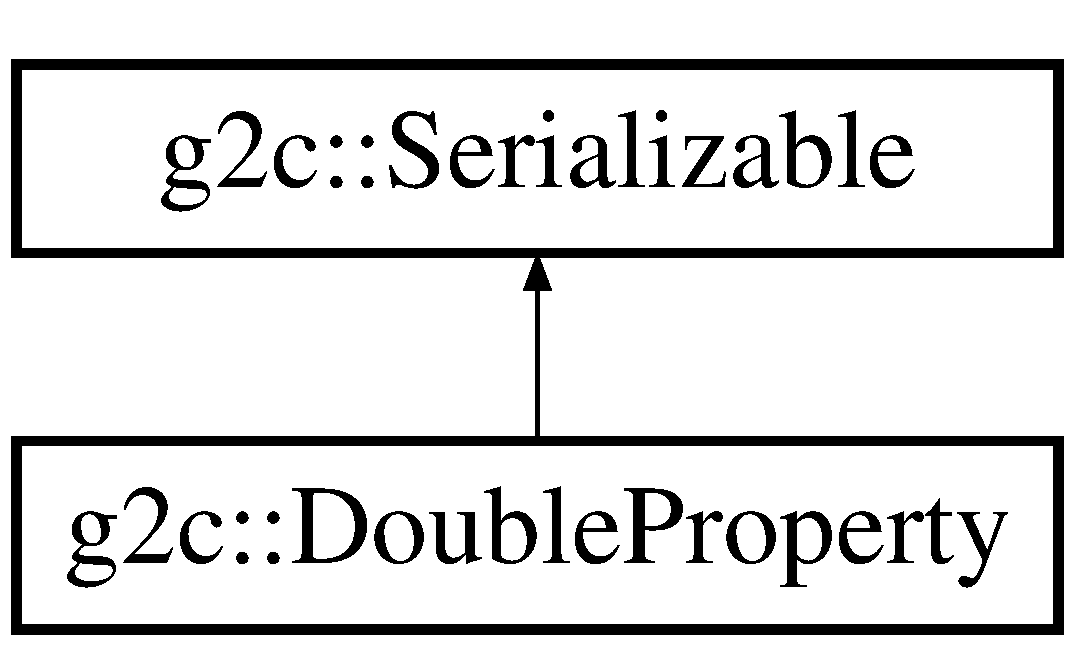
\includegraphics[height=2cm]{classg2c_1_1_double_property}
\end{center}
\end{figure}
\subsection*{Public Member Functions}
\begin{DoxyCompactItemize}
\item 
\hypertarget{classg2c_1_1_double_property_a06be4c1ebf4ca027d8f4d843f42a78aa}{
{\bfseries DoubleProperty} (double x)}
\label{classg2c_1_1_double_property_a06be4c1ebf4ca027d8f4d843f42a78aa}

\item 
\hypertarget{classg2c_1_1_double_property_a3c585d2853693e8fe944fbc6eaeffbcf}{
virtual std::string {\bfseries serialize} (std::string indent=\char`\"{}\char`\"{}) const }
\label{classg2c_1_1_double_property_a3c585d2853693e8fe944fbc6eaeffbcf}

\item 
\hypertarget{classg2c_1_1_double_property_a9142cfcebfeca44ee6214a70b0573646}{
virtual void {\bfseries initWithParseNode} (const \hyperlink{classparse_1_1_node}{parse::Node} $\ast$n)}
\label{classg2c_1_1_double_property_a9142cfcebfeca44ee6214a70b0573646}

\item 
\hypertarget{classg2c_1_1_double_property_af051aa7b216ed9342355cbcd42d6594a}{
bool {\bfseries operator==} (double t) const }
\label{classg2c_1_1_double_property_af051aa7b216ed9342355cbcd42d6594a}

\item 
\hypertarget{classg2c_1_1_double_property_a15931d4718650131417069ebebf64194}{
bool {\bfseries operator!=} (double t) const }
\label{classg2c_1_1_double_property_a15931d4718650131417069ebebf64194}

\item 
\hypertarget{classg2c_1_1_double_property_a4d8032444533ab67842bac7bc62aa818}{
double {\bfseries operator()} () const }
\label{classg2c_1_1_double_property_a4d8032444533ab67842bac7bc62aa818}

\item 
\hypertarget{classg2c_1_1_double_property_ac5f0d9704a186960e7af8f559bb46e9b}{
void {\bfseries operator()} (double x)}
\label{classg2c_1_1_double_property_ac5f0d9704a186960e7af8f559bb46e9b}

\item 
\hypertarget{classg2c_1_1_double_property_a2cfa1646b9425b5edd8909689af1d2bf}{
{\bfseries operator double \&} ()}
\label{classg2c_1_1_double_property_a2cfa1646b9425b5edd8909689af1d2bf}

\item 
\hypertarget{classg2c_1_1_double_property_a87af6f1429ad43df5655dc5ff35418be}{
{\bfseries operator double const \&} () const }
\label{classg2c_1_1_double_property_a87af6f1429ad43df5655dc5ff35418be}

\end{DoxyCompactItemize}


The documentation for this class was generated from the following files:\begin{DoxyCompactItemize}
\item 
serializable.h\item 
serializable.cpp\end{DoxyCompactItemize}

\hypertarget{classg2c_1_1_effect}{
\section{g2c::Effect Class Reference}
\label{classg2c_1_1_effect}\index{g2c::Effect@{g2c::Effect}}
}
Inheritance diagram for g2c::Effect::\begin{figure}[H]
\begin{center}
\leavevmode
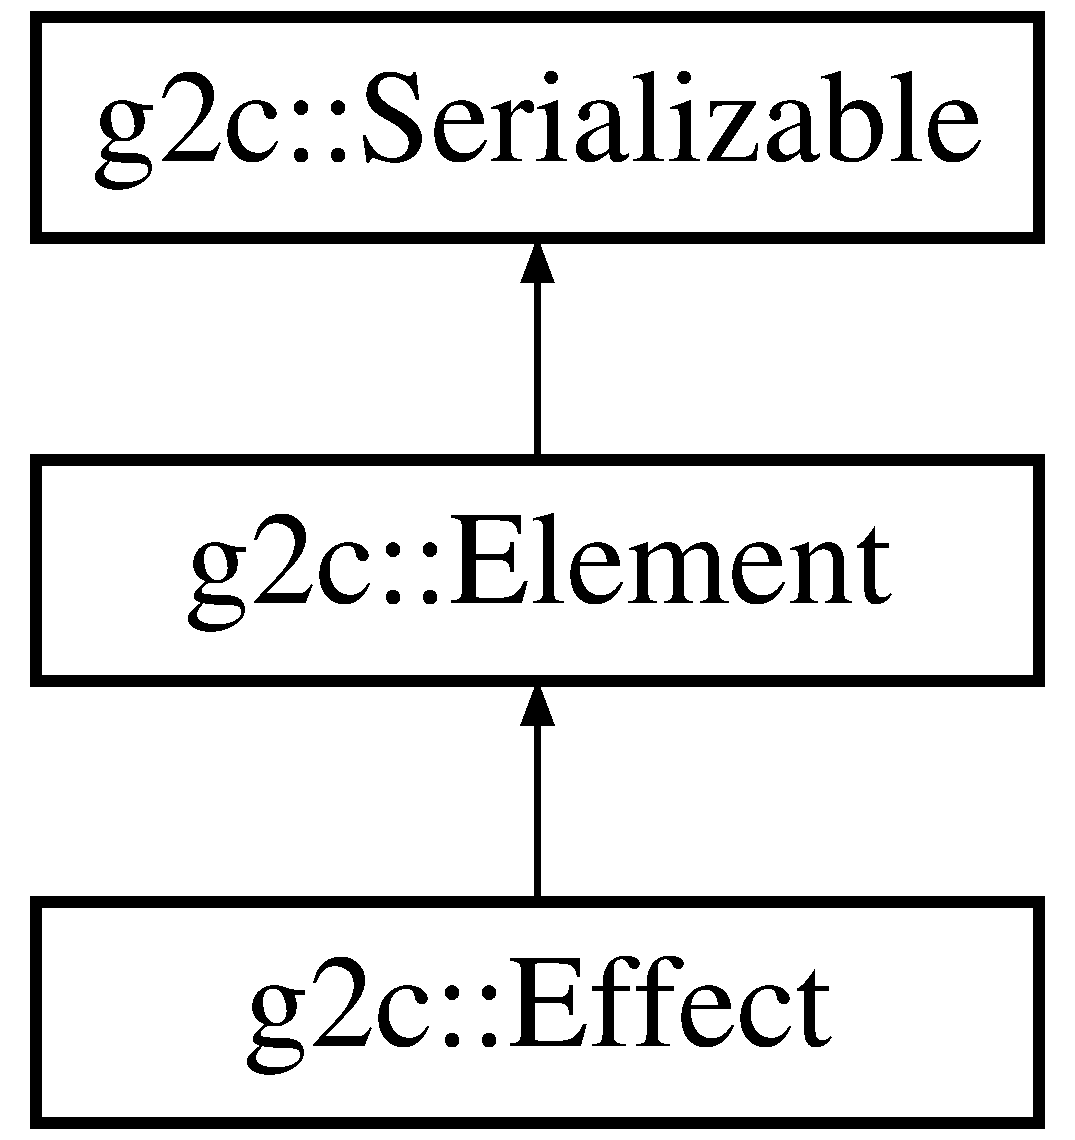
\includegraphics[height=3cm]{classg2c_1_1_effect}
\end{center}
\end{figure}
\subsection*{Public Member Functions}
\begin{DoxyCompactItemize}
\item 
\hypertarget{classg2c_1_1_effect_a45756da886e9c18f4ff413d9fe65b816}{
void {\bfseries compile} ()}
\label{classg2c_1_1_effect_a45756da886e9c18f4ff413d9fe65b816}

\end{DoxyCompactItemize}
\subsection*{Public Attributes}
\begin{DoxyCompactItemize}
\item 
\hypertarget{classg2c_1_1_effect_aae881ae57bd71da9ac5164c999e1ee81}{
std::string {\bfseries vertexCode}}
\label{classg2c_1_1_effect_aae881ae57bd71da9ac5164c999e1ee81}

\item 
\hypertarget{classg2c_1_1_effect_a3e199003cbbe8f3cc4fc1388538dcdd3}{
std::string {\bfseries fragmentCode}}
\label{classg2c_1_1_effect_a3e199003cbbe8f3cc4fc1388538dcdd3}

\end{DoxyCompactItemize}
\subsection*{Protected Member Functions}
\begin{DoxyCompactItemize}
\item 
\hypertarget{classg2c_1_1_effect_a408741daf26cb37c8da6153e6dfa505e}{
virtual std::string {\bfseries serializeElements} (std::string indent=\char`\"{}\char`\"{}) const }
\label{classg2c_1_1_effect_a408741daf26cb37c8da6153e6dfa505e}

\item 
\hypertarget{classg2c_1_1_effect_a30f051df920e9c81d81a775318e2d053}{
virtual void {\bfseries handleChild} (const \hyperlink{classparse_1_1_node}{parse::Node} $\ast$n)}
\label{classg2c_1_1_effect_a30f051df920e9c81d81a775318e2d053}

\end{DoxyCompactItemize}
\subsection*{Friends}
\begin{DoxyCompactItemize}
\item 
\hypertarget{classg2c_1_1_effect_a9aca7b7350e6ffa0e2d6320834ad1857}{
class {\bfseries Geometry}}
\label{classg2c_1_1_effect_a9aca7b7350e6ffa0e2d6320834ad1857}

\item 
\hypertarget{classg2c_1_1_effect_a1e1ef8352d0a310bace7f7a3307d1378}{
class {\bfseries Shape}}
\label{classg2c_1_1_effect_a1e1ef8352d0a310bace7f7a3307d1378}

\end{DoxyCompactItemize}


The documentation for this class was generated from the following files:\begin{DoxyCompactItemize}
\item 
graphics.h\item 
graphics.cpp\end{DoxyCompactItemize}

\hypertarget{classg2c_1_1_element}{
\section{g2c::Element Class Reference}
\label{classg2c_1_1_element}\index{g2c::Element@{g2c::Element}}
}
Inheritance diagram for g2c::Element::\begin{figure}[H]
\begin{center}
\leavevmode
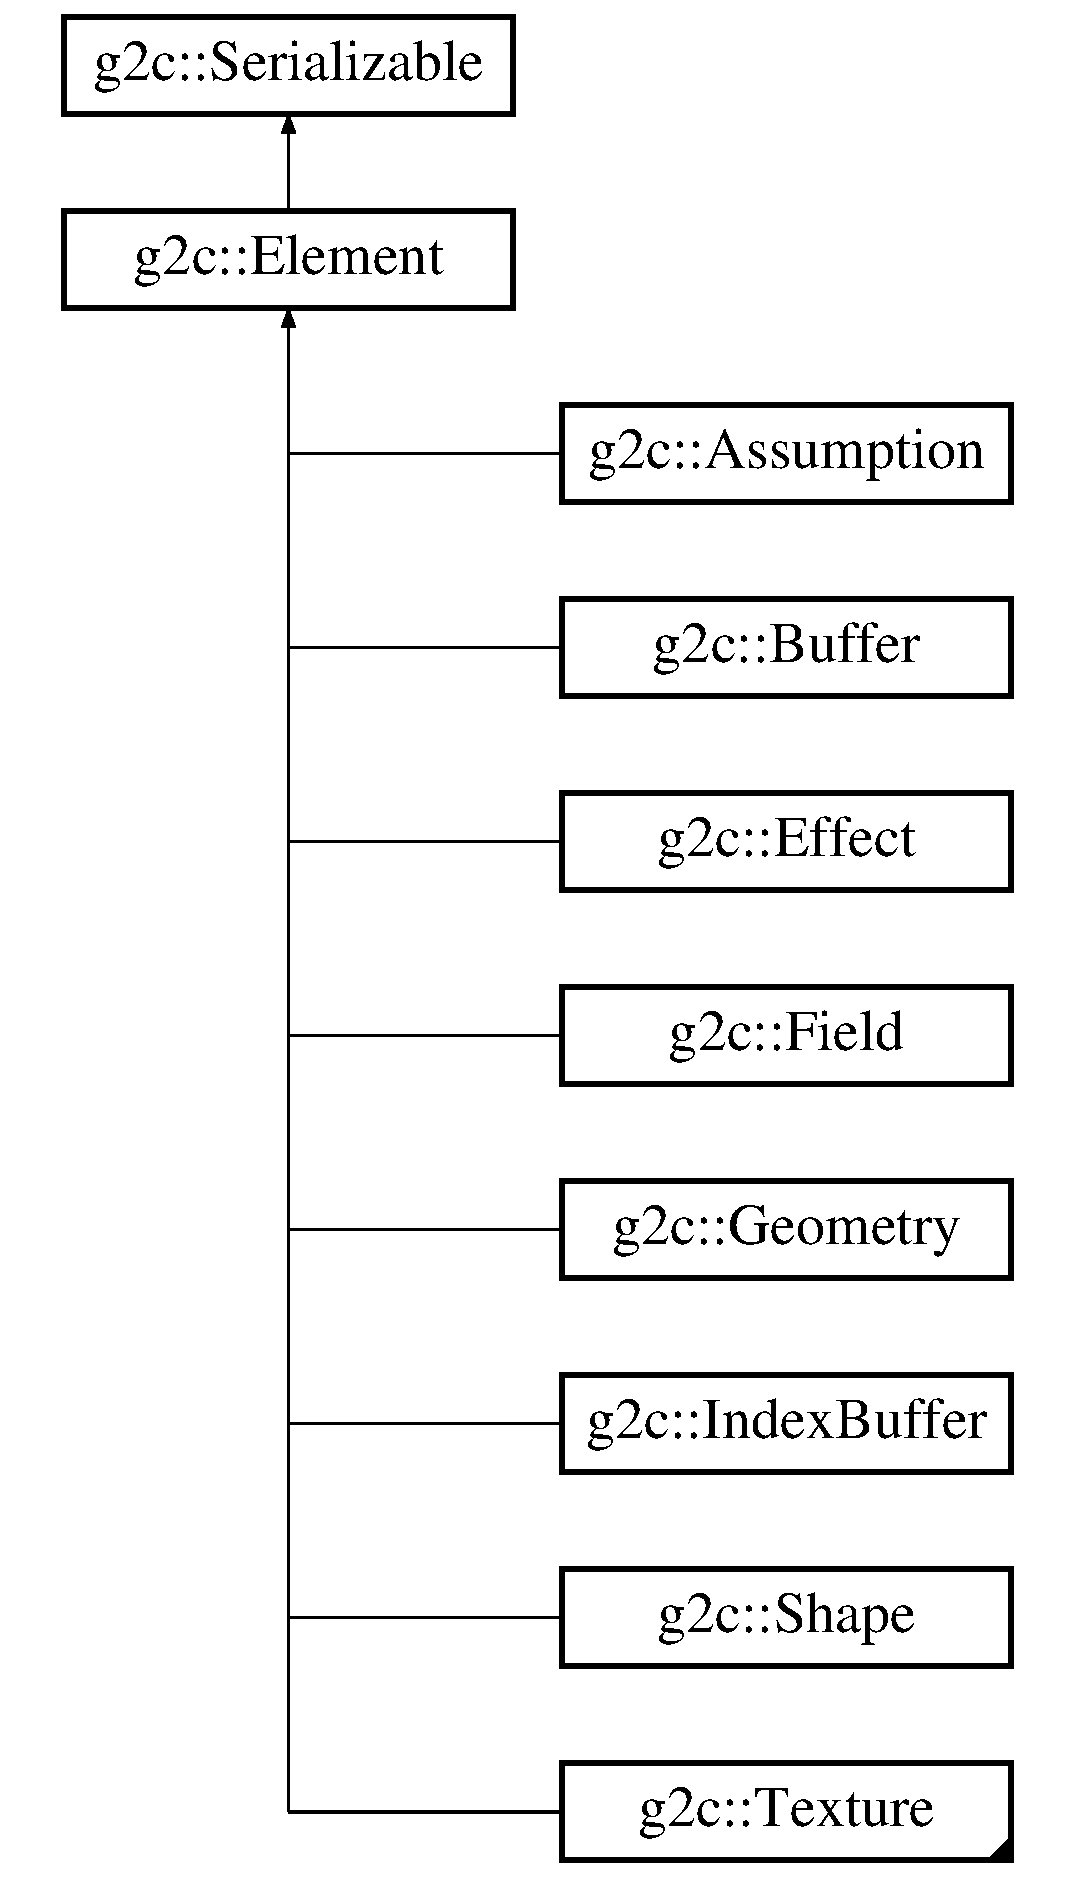
\includegraphics[height=10cm]{classg2c_1_1_element}
\end{center}
\end{figure}


The documentation for this class was generated from the following file:\begin{DoxyCompactItemize}
\item 
element.h\end{DoxyCompactItemize}

\hypertarget{classg2c_1_1_fade_in}{
\section{g2c::FadeIn Class Reference}
\label{classg2c_1_1_fade_in}\index{g2c::FadeIn@{g2c::FadeIn}}
}
Inheritance diagram for g2c::FadeIn::\begin{figure}[H]
\begin{center}
\leavevmode
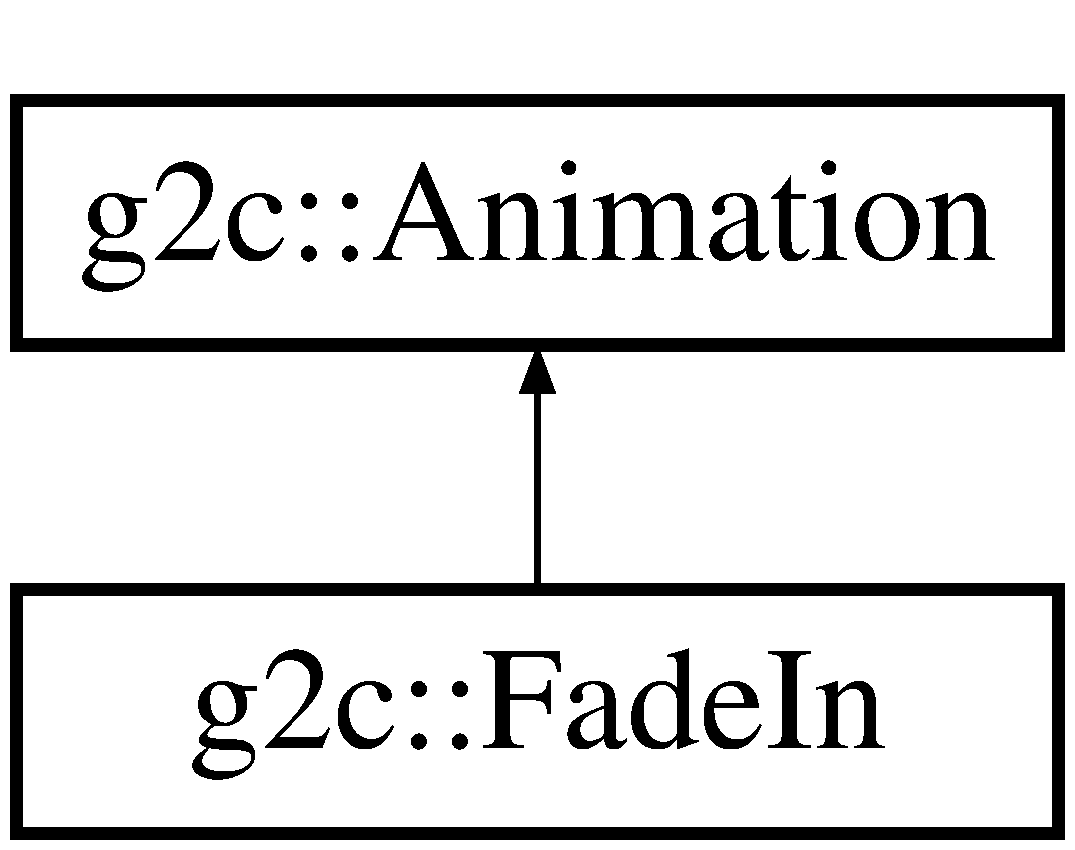
\includegraphics[height=2cm]{classg2c_1_1_fade_in}
\end{center}
\end{figure}
\subsection*{Public Member Functions}
\begin{DoxyCompactItemize}
\item 
\hypertarget{classg2c_1_1_fade_in_aa4692c7057e12566f994852da29d62ea}{
{\bfseries FadeIn} (double instart, double induration, \hyperlink{classg2c_1_1_node}{Node} $\ast$node, bool inStopsEvents=true)}
\label{classg2c_1_1_fade_in_aa4692c7057e12566f994852da29d62ea}

\item 
\hypertarget{classg2c_1_1_fade_in_ae175bff38735f9623785e967d2c6f89d}{
virtual void {\bfseries begin} ()}
\label{classg2c_1_1_fade_in_ae175bff38735f9623785e967d2c6f89d}

\item 
\hypertarget{classg2c_1_1_fade_in_a74f9cb7931f6467b57ffcae832f717a1}{
virtual void {\bfseries step} (double t)}
\label{classg2c_1_1_fade_in_a74f9cb7931f6467b57ffcae832f717a1}

\item 
\hypertarget{classg2c_1_1_fade_in_aae92e1974d3ceb722236a8210971280a}{
virtual void {\bfseries end} ()}
\label{classg2c_1_1_fade_in_aae92e1974d3ceb722236a8210971280a}

\end{DoxyCompactItemize}
\subsection*{Public Attributes}
\begin{DoxyCompactItemize}
\item 
\hypertarget{classg2c_1_1_fade_in_ab62d93a61763af15b0bc322c7a9b8475}{
\hyperlink{classg2c_1_1_node}{Node} $\ast$ {\bfseries node}}
\label{classg2c_1_1_fade_in_ab62d93a61763af15b0bc322c7a9b8475}

\end{DoxyCompactItemize}


The documentation for this class was generated from the following files:\begin{DoxyCompactItemize}
\item 
animations.h\item 
animations.cpp\end{DoxyCompactItemize}

\hypertarget{classg2c_1_1_fade_out}{
\section{g2c::FadeOut Class Reference}
\label{classg2c_1_1_fade_out}\index{g2c::FadeOut@{g2c::FadeOut}}
}
Inheritance diagram for g2c::FadeOut::\begin{figure}[H]
\begin{center}
\leavevmode
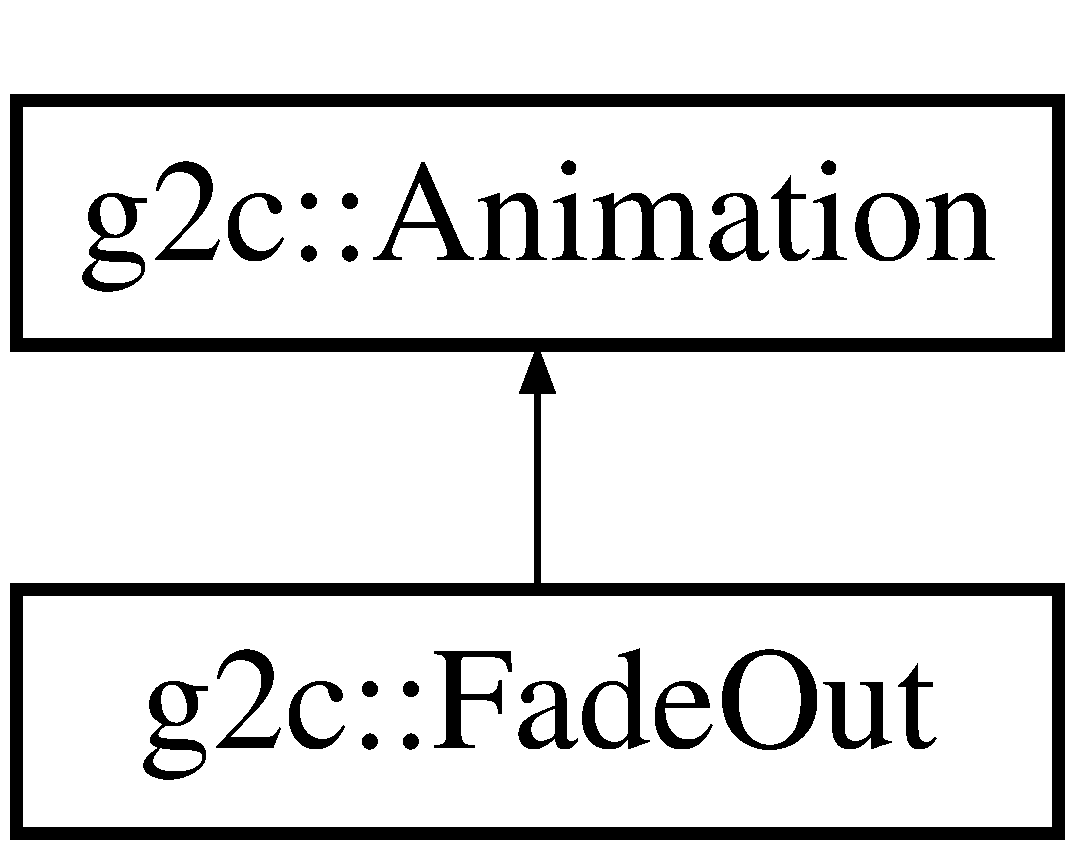
\includegraphics[height=2cm]{classg2c_1_1_fade_out}
\end{center}
\end{figure}
\subsection*{Public Member Functions}
\begin{DoxyCompactItemize}
\item 
\hypertarget{classg2c_1_1_fade_out_a41c6fefd44e5bd35925298ec821d9303}{
{\bfseries FadeOut} (double instart, double induration, \hyperlink{classg2c_1_1_node}{Node} $\ast$node, bool inStopsEvents=true)}
\label{classg2c_1_1_fade_out_a41c6fefd44e5bd35925298ec821d9303}

\item 
\hypertarget{classg2c_1_1_fade_out_a6879b534e78f9ea3449e2826d3fae279}{
virtual void {\bfseries begin} ()}
\label{classg2c_1_1_fade_out_a6879b534e78f9ea3449e2826d3fae279}

\item 
\hypertarget{classg2c_1_1_fade_out_a187ad5e8189335250d6c23018fb72e41}{
virtual void {\bfseries step} (double t)}
\label{classg2c_1_1_fade_out_a187ad5e8189335250d6c23018fb72e41}

\item 
\hypertarget{classg2c_1_1_fade_out_a2ee780b3192dcc478ce0171c1cdd5f3f}{
virtual void {\bfseries end} ()}
\label{classg2c_1_1_fade_out_a2ee780b3192dcc478ce0171c1cdd5f3f}

\end{DoxyCompactItemize}
\subsection*{Public Attributes}
\begin{DoxyCompactItemize}
\item 
\hypertarget{classg2c_1_1_fade_out_aeb2f3efc76b0afdebdd827b39dc4b60f}{
\hyperlink{classg2c_1_1_node}{Node} $\ast$ {\bfseries node}}
\label{classg2c_1_1_fade_out_aeb2f3efc76b0afdebdd827b39dc4b60f}

\end{DoxyCompactItemize}


The documentation for this class was generated from the following files:\begin{DoxyCompactItemize}
\item 
animations.h\item 
animations.cpp\end{DoxyCompactItemize}

\hypertarget{classg2c_1_1_field}{
\section{g2c::Field Class Reference}
\label{classg2c_1_1_field}\index{g2c::Field@{g2c::Field}}
}
Inheritance diagram for g2c::Field::\begin{figure}[H]
\begin{center}
\leavevmode
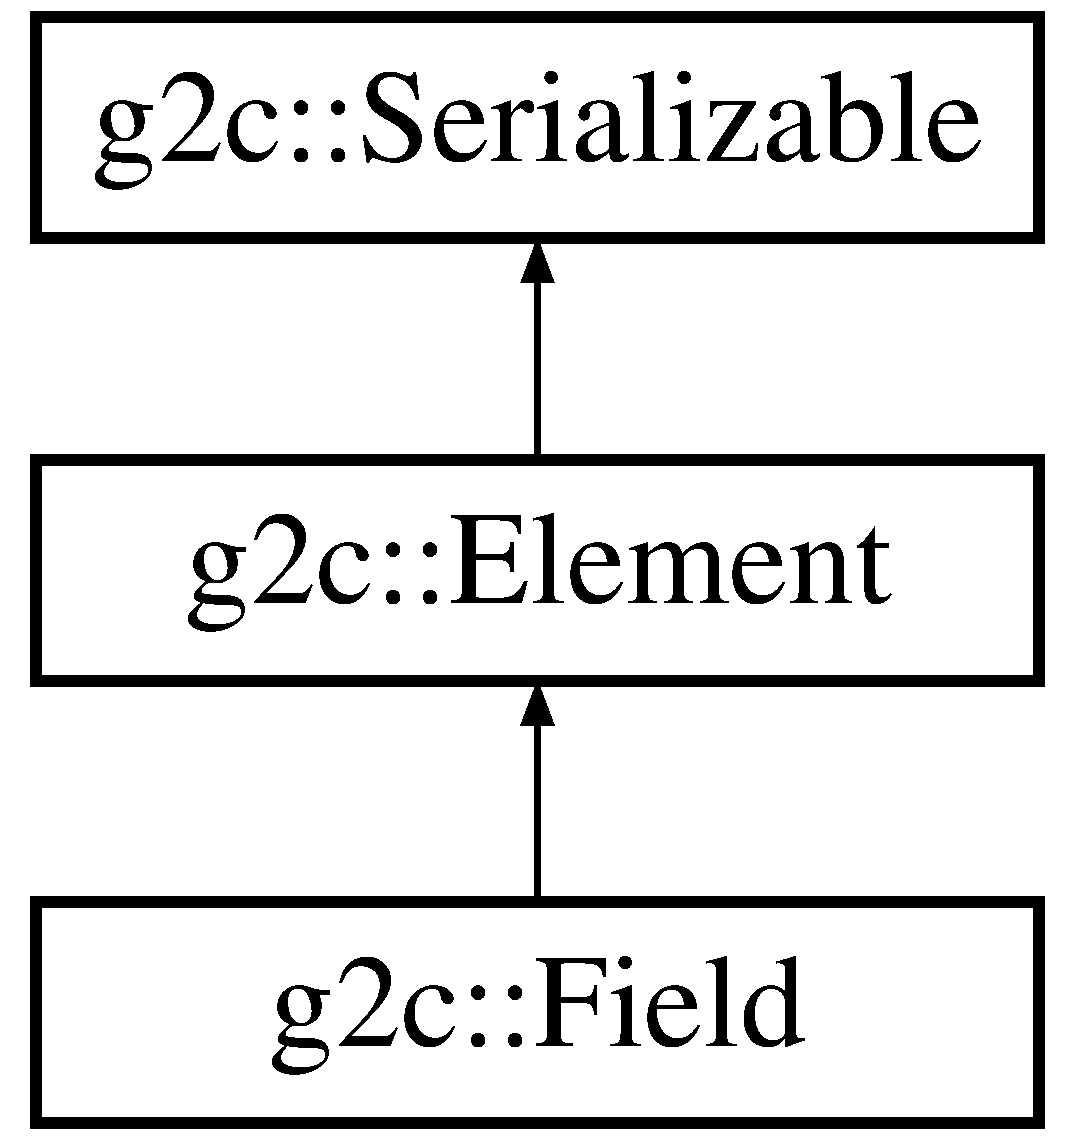
\includegraphics[height=3cm]{classg2c_1_1_field}
\end{center}
\end{figure}
\subsection*{Public Member Functions}
\begin{DoxyCompactItemize}
\item 
\hypertarget{classg2c_1_1_field_a45932bbf099d28660b010db9c6d17c00}{
{\bfseries Field} (const \hyperlink{classg2c_1_1_buffer}{Buffer} $\ast$buffer, GLint size, GLsizei stride=0, int offset=0)}
\label{classg2c_1_1_field_a45932bbf099d28660b010db9c6d17c00}

\end{DoxyCompactItemize}
\subsection*{Public Attributes}
\begin{DoxyCompactItemize}
\item 
\hypertarget{classg2c_1_1_field_a34877f3f69bd46424d88ec61f9d02da4}{
std::string {\bfseries bufferName}}
\label{classg2c_1_1_field_a34877f3f69bd46424d88ec61f9d02da4}

\item 
\hypertarget{classg2c_1_1_field_aae940634905af081ccc8dd1e3531c1ac}{
const \hyperlink{classg2c_1_1_buffer}{Buffer} $\ast$ {\bfseries buffer}}
\label{classg2c_1_1_field_aae940634905af081ccc8dd1e3531c1ac}

\end{DoxyCompactItemize}
\subsection*{Protected Member Functions}
\begin{DoxyCompactItemize}
\item 
\hypertarget{classg2c_1_1_field_afb63850b58d85cc453b92ae33b6daffc}{
virtual std::string {\bfseries serializeElements} (std::string indent=\char`\"{}\char`\"{}) const }
\label{classg2c_1_1_field_afb63850b58d85cc453b92ae33b6daffc}

\item 
\hypertarget{classg2c_1_1_field_a3ad80573ea120cd6fda91eaff0a246e9}{
virtual void {\bfseries handleChild} (const \hyperlink{classparse_1_1_node}{parse::Node} $\ast$n)}
\label{classg2c_1_1_field_a3ad80573ea120cd6fda91eaff0a246e9}

\end{DoxyCompactItemize}
\subsection*{Friends}
\begin{DoxyCompactItemize}
\item 
\hypertarget{classg2c_1_1_field_ac8649272bb0576cc72f2486439664efe}{
class {\bfseries Effect}}
\label{classg2c_1_1_field_ac8649272bb0576cc72f2486439664efe}

\end{DoxyCompactItemize}


The documentation for this class was generated from the following files:\begin{DoxyCompactItemize}
\item 
graphics.h\item 
graphics.cpp\end{DoxyCompactItemize}

\hypertarget{classg2c_1_1_font}{
\section{g2c::Font Class Reference}
\label{classg2c_1_1_font}\index{g2c::Font@{g2c::Font}}
}


{\ttfamily \#include $<$sprites.h$>$}Inheritance diagram for g2c::Font::\begin{figure}[H]
\begin{center}
\leavevmode
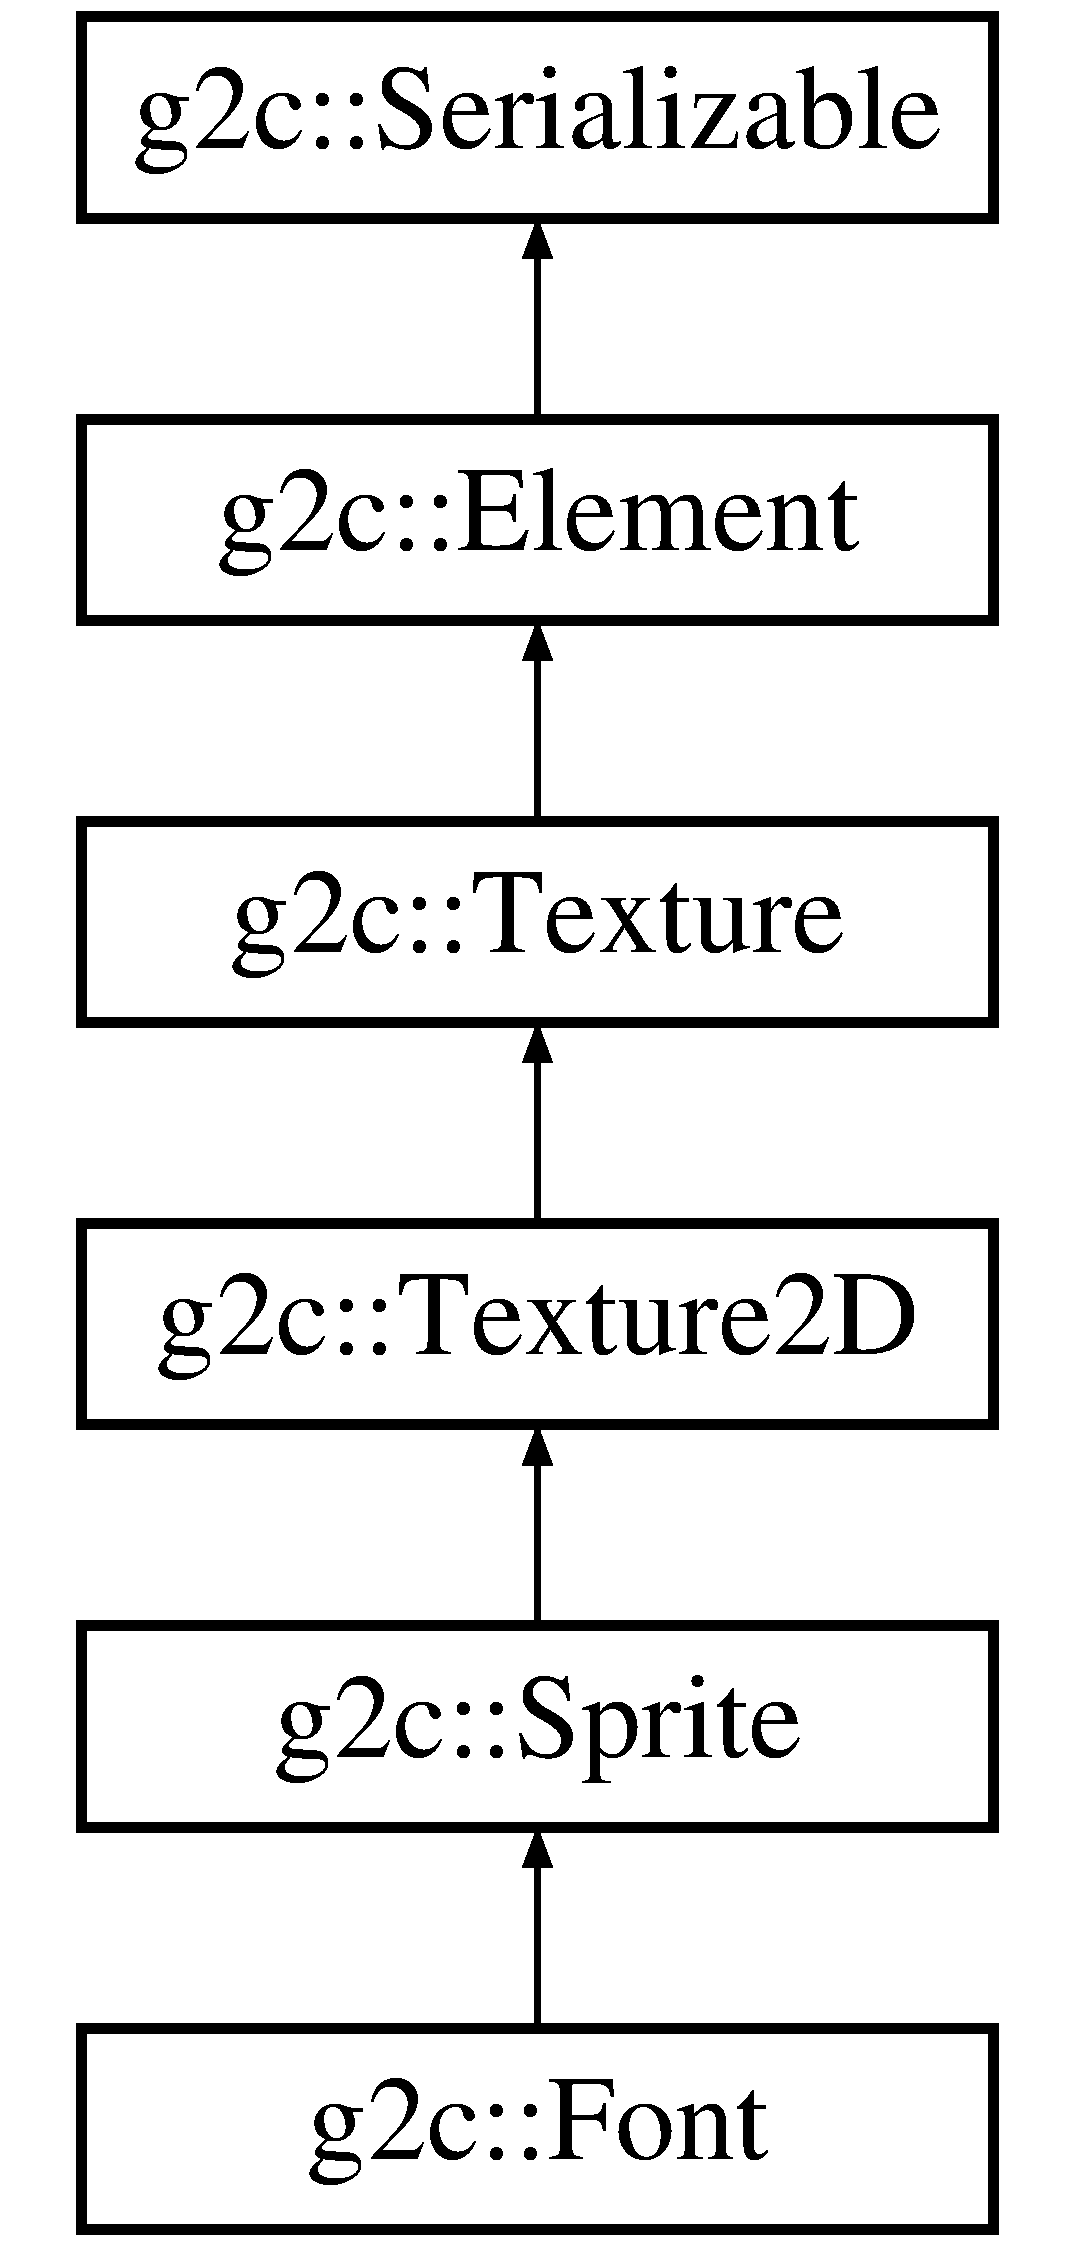
\includegraphics[height=6cm]{classg2c_1_1_font}
\end{center}
\end{figure}
\subsection*{Public Member Functions}
\begin{DoxyCompactItemize}
\item 
\hypertarget{classg2c_1_1_font_aa03376086a0e53e02025277774d4f926}{
double {\bfseries charWidth} (char c) const }
\label{classg2c_1_1_font_aa03376086a0e53e02025277774d4f926}

\item 
\hypertarget{classg2c_1_1_font_a2ac044478305dfd8447c7ba05da0bbcc}{
double {\bfseries charLeft} (char c) const }
\label{classg2c_1_1_font_a2ac044478305dfd8447c7ba05da0bbcc}

\item 
\hypertarget{classg2c_1_1_font_a5712609addff68f271d091e1d3174b0f}{
double {\bfseries lineWidth} (double k, const char $\ast$s, int startIndex) const }
\label{classg2c_1_1_font_a5712609addff68f271d091e1d3174b0f}

\item 
\hypertarget{classg2c_1_1_font_ac47823fde56a234c1c73a479b9eab032}{
std::vector$<$ std::pair$<$ int, int $>$ $>$ {\bfseries lineIndices} (const char $\ast$s) const }
\label{classg2c_1_1_font_ac47823fde56a234c1c73a479b9eab032}

\item 
\hypertarget{classg2c_1_1_font_a7e41d610dbead7da5fadd91f2036ae70}{
void {\bfseries drawString} (const Mat4 \&M, const \hyperlink{classg2c_1_1_color}{Color} \&color, double x, double y, double k, const char $\ast$s, const std::string \&justification=\char`\"{}left\char`\"{}) const }
\label{classg2c_1_1_font_a7e41d610dbead7da5fadd91f2036ae70}

\item 
\hypertarget{classg2c_1_1_font_a8063875af4363343687651fcbc62b917}{
\hyperlink{classg2c_1_1_polygon}{Polygon} {\bfseries stringRectangle} (double k, const char $\ast$s, const std::string \&justification=\char`\"{}left\char`\"{}) const }
\label{classg2c_1_1_font_a8063875af4363343687651fcbc62b917}

\item 
\hypertarget{classg2c_1_1_font_ab866a90a5af638bae26b0f92e48f5046}{
void {\bfseries getWidthsFromBitmap} (const \hyperlink{classg2c_1_1_bitmap}{Bitmap} \&bitmap)}
\label{classg2c_1_1_font_ab866a90a5af638bae26b0f92e48f5046}

\item 
\hypertarget{classg2c_1_1_font_a719d933e2be93c8f8d185451e86bf635}{
virtual std::string {\bfseries serializeElements} (std::string indent=\char`\"{}\char`\"{}) const }
\label{classg2c_1_1_font_a719d933e2be93c8f8d185451e86bf635}

\item 
\hypertarget{classg2c_1_1_font_a2d29920e2f73a9b1eee9fdb452516664}{
virtual void {\bfseries handleChild} (const \hyperlink{classparse_1_1_node}{parse::Node} $\ast$n)}
\label{classg2c_1_1_font_a2d29920e2f73a9b1eee9fdb452516664}

\end{DoxyCompactItemize}
\subsection*{Public Attributes}
\begin{DoxyCompactItemize}
\item 
\hypertarget{classg2c_1_1_font_ad5ebe530ff4f227a19f8ca1efb2103b3}{
std::vector$<$ double $>$ {\bfseries widths}}
\label{classg2c_1_1_font_ad5ebe530ff4f227a19f8ca1efb2103b3}

\item 
\hypertarget{classg2c_1_1_font_a19fd7b96afc081f6ce2d1d56e7704586}{
std::vector$<$ double $>$ {\bfseries lefts}}
\label{classg2c_1_1_font_a19fd7b96afc081f6ce2d1d56e7704586}

\item 
\hypertarget{classg2c_1_1_font_ae29b567190687d5be84898462871671b}{
double {\bfseries lineHeight}}
\label{classg2c_1_1_font_ae29b567190687d5be84898462871671b}

\item 
\hypertarget{classg2c_1_1_font_ace21eb427461d59c70ca4bdb3b64bbde}{
double {\bfseries lineBottom}}
\label{classg2c_1_1_font_ace21eb427461d59c70ca4bdb3b64bbde}

\item 
\hypertarget{classg2c_1_1_font_acb98fb00e0258413c689721b26f511d9}{
double {\bfseries widthScale}}
\label{classg2c_1_1_font_acb98fb00e0258413c689721b26f511d9}

\item 
\hypertarget{classg2c_1_1_font_ae3f4396bdc9acee5681e2cee879106e9}{
double {\bfseries spacing}}
\label{classg2c_1_1_font_ae3f4396bdc9acee5681e2cee879106e9}

\item 
\hypertarget{classg2c_1_1_font_a27b77d89290e4bc1eee4d34edd152b8d}{
char {\bfseries baseChar}}
\label{classg2c_1_1_font_a27b77d89290e4bc1eee4d34edd152b8d}

\end{DoxyCompactItemize}


\subsection{Detailed Description}
\hyperlink{classg2c_1_1_font}{Font} is a type of \hyperlink{classg2c_1_1_sprite}{Sprite} which contains images of characters. Whereas a sprite contains frames of animation and is drawn using an \hyperlink{classg2c_1_1_actor}{Actor}, \hyperlink{classg2c_1_1_font}{Font} contains as its frames images of characters, and is drawn using a \hyperlink{classg2c_1_1_text}{Text} object. 

The documentation for this class was generated from the following files:\begin{DoxyCompactItemize}
\item 
sprites.h\item 
sprites.cpp\end{DoxyCompactItemize}

\hypertarget{classg2c_1_1_geometry}{
\section{g2c::Geometry Class Reference}
\label{classg2c_1_1_geometry}\index{g2c::Geometry@{g2c::Geometry}}
}
Inheritance diagram for g2c::Geometry::\begin{figure}[H]
\begin{center}
\leavevmode
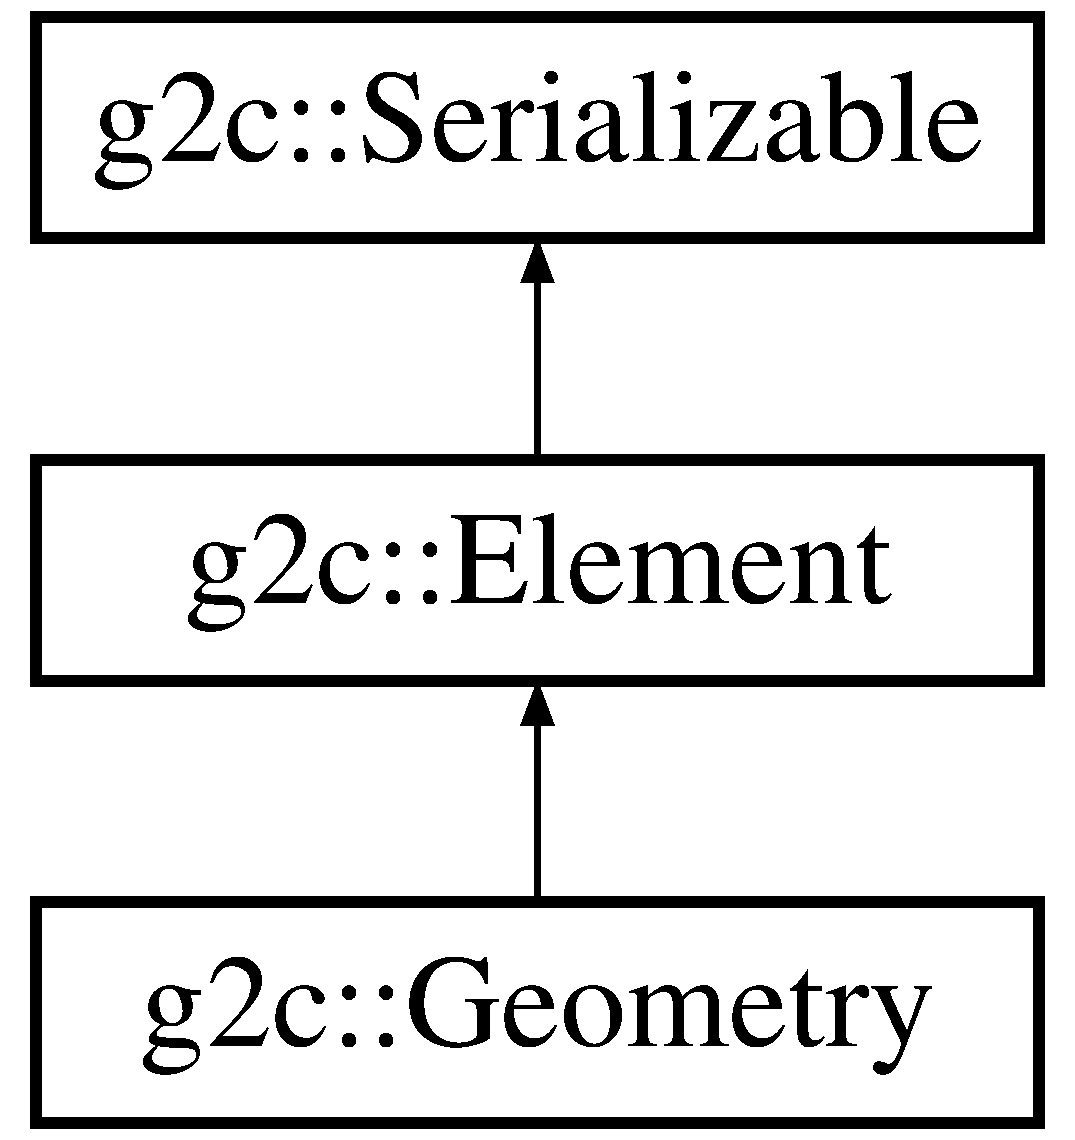
\includegraphics[height=3cm]{classg2c_1_1_geometry}
\end{center}
\end{figure}
\subsection*{Public Member Functions}
\begin{DoxyCompactItemize}
\item 
\hypertarget{classg2c_1_1_geometry_a0fddf5dee834d1b3c8e2dc3d3e3b9557}{
void {\bfseries draw} () const }
\label{classg2c_1_1_geometry_a0fddf5dee834d1b3c8e2dc3d3e3b9557}

\end{DoxyCompactItemize}
\subsection*{Public Attributes}
\begin{DoxyCompactItemize}
\item 
\hypertarget{classg2c_1_1_geometry_afeec577d78767205f4be6b50626d87c6}{
std::string {\bfseries indicesName}}
\label{classg2c_1_1_geometry_afeec577d78767205f4be6b50626d87c6}

\item 
\hypertarget{classg2c_1_1_geometry_ae1d3cd504bfe1d2a9afea2f5fff7aa53}{
const \hyperlink{classg2c_1_1_index_buffer}{IndexBuffer} $\ast$ {\bfseries indices}}
\label{classg2c_1_1_geometry_ae1d3cd504bfe1d2a9afea2f5fff7aa53}

\end{DoxyCompactItemize}
\subsection*{Protected Member Functions}
\begin{DoxyCompactItemize}
\item 
\hypertarget{classg2c_1_1_geometry_ad2734a4bb00c779bcb2076671d8eba15}{
virtual std::string {\bfseries serializeElements} (std::string indent=\char`\"{}\char`\"{}) const }
\label{classg2c_1_1_geometry_ad2734a4bb00c779bcb2076671d8eba15}

\item 
\hypertarget{classg2c_1_1_geometry_ae074d5d8b972f3ad53ed42b381935f57}{
virtual void {\bfseries handleChild} (const \hyperlink{classparse_1_1_node}{parse::Node} $\ast$n)}
\label{classg2c_1_1_geometry_ae074d5d8b972f3ad53ed42b381935f57}

\end{DoxyCompactItemize}
\subsection*{Friends}
\begin{DoxyCompactItemize}
\item 
\hypertarget{classg2c_1_1_geometry_a1e1ef8352d0a310bace7f7a3307d1378}{
class {\bfseries Shape}}
\label{classg2c_1_1_geometry_a1e1ef8352d0a310bace7f7a3307d1378}

\end{DoxyCompactItemize}


The documentation for this class was generated from the following files:\begin{DoxyCompactItemize}
\item 
graphics.h\item 
graphics.cpp\end{DoxyCompactItemize}

\hypertarget{classg2c_1_1_index_buffer}{
\section{g2c::IndexBuffer Class Reference}
\label{classg2c_1_1_index_buffer}\index{g2c::IndexBuffer@{g2c::IndexBuffer}}
}
Inheritance diagram for g2c::IndexBuffer::\begin{figure}[H]
\begin{center}
\leavevmode
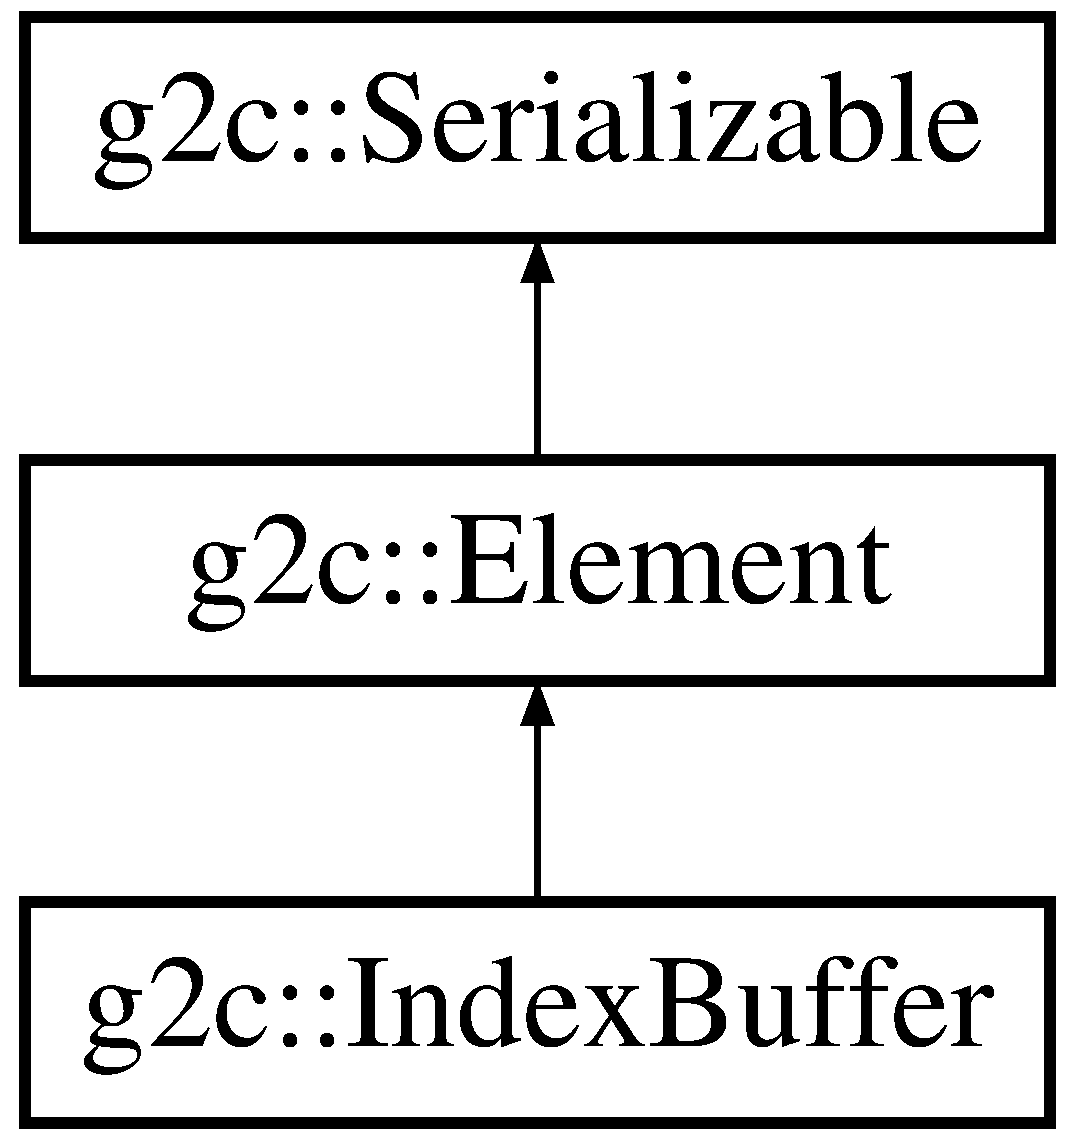
\includegraphics[height=3cm]{classg2c_1_1_index_buffer}
\end{center}
\end{figure}
\subsection*{Public Member Functions}
\begin{DoxyCompactItemize}
\item 
\hypertarget{classg2c_1_1_index_buffer_aa311924a9d7de1e0f3990691d157faea}{
{\bfseries IndexBuffer} (const std::vector$<$ int $>$ \&v)}
\label{classg2c_1_1_index_buffer_aa311924a9d7de1e0f3990691d157faea}

\item 
\hypertarget{classg2c_1_1_index_buffer_aafb41457cb70feda11f3f43bbdc13535}{
{\bfseries IndexBuffer} (const std::vector$<$ unsigned short $>$ \&v)}
\label{classg2c_1_1_index_buffer_aafb41457cb70feda11f3f43bbdc13535}

\item 
\hypertarget{classg2c_1_1_index_buffer_a307318d26def8baeabb6b5756fafd3e7}{
{\bfseries IndexBuffer} (const int $\ast$v, int size)}
\label{classg2c_1_1_index_buffer_a307318d26def8baeabb6b5756fafd3e7}

\item 
\hypertarget{classg2c_1_1_index_buffer_a73cb82148ae19088e0e93b90190bded9}{
{\bfseries IndexBuffer} (const unsigned short $\ast$v, int size)}
\label{classg2c_1_1_index_buffer_a73cb82148ae19088e0e93b90190bded9}

\end{DoxyCompactItemize}
\subsection*{Protected Member Functions}
\begin{DoxyCompactItemize}
\item 
\hypertarget{classg2c_1_1_index_buffer_a71b7b8742269322b6beb4cc49c6187b3}{
virtual std::string {\bfseries serializeElements} (std::string indent=\char`\"{}\char`\"{}) const }
\label{classg2c_1_1_index_buffer_a71b7b8742269322b6beb4cc49c6187b3}

\item 
\hypertarget{classg2c_1_1_index_buffer_ab8108ac228531a7d14e20f1163a5756d}{
virtual void {\bfseries handleChild} (const \hyperlink{classparse_1_1_node}{parse::Node} $\ast$n)}
\label{classg2c_1_1_index_buffer_ab8108ac228531a7d14e20f1163a5756d}

\end{DoxyCompactItemize}
\subsection*{Friends}
\begin{DoxyCompactItemize}
\item 
\hypertarget{classg2c_1_1_index_buffer_a9aca7b7350e6ffa0e2d6320834ad1857}{
class {\bfseries Geometry}}
\label{classg2c_1_1_index_buffer_a9aca7b7350e6ffa0e2d6320834ad1857}

\end{DoxyCompactItemize}


The documentation for this class was generated from the following files:\begin{DoxyCompactItemize}
\item 
graphics.h\item 
graphics.cpp\end{DoxyCompactItemize}

\hypertarget{classg2c_1_1_integer}{
\section{g2c::Integer Class Reference}
\label{classg2c_1_1_integer}\index{g2c::Integer@{g2c::Integer}}
}
Inheritance diagram for g2c::Integer::\begin{figure}[H]
\begin{center}
\leavevmode
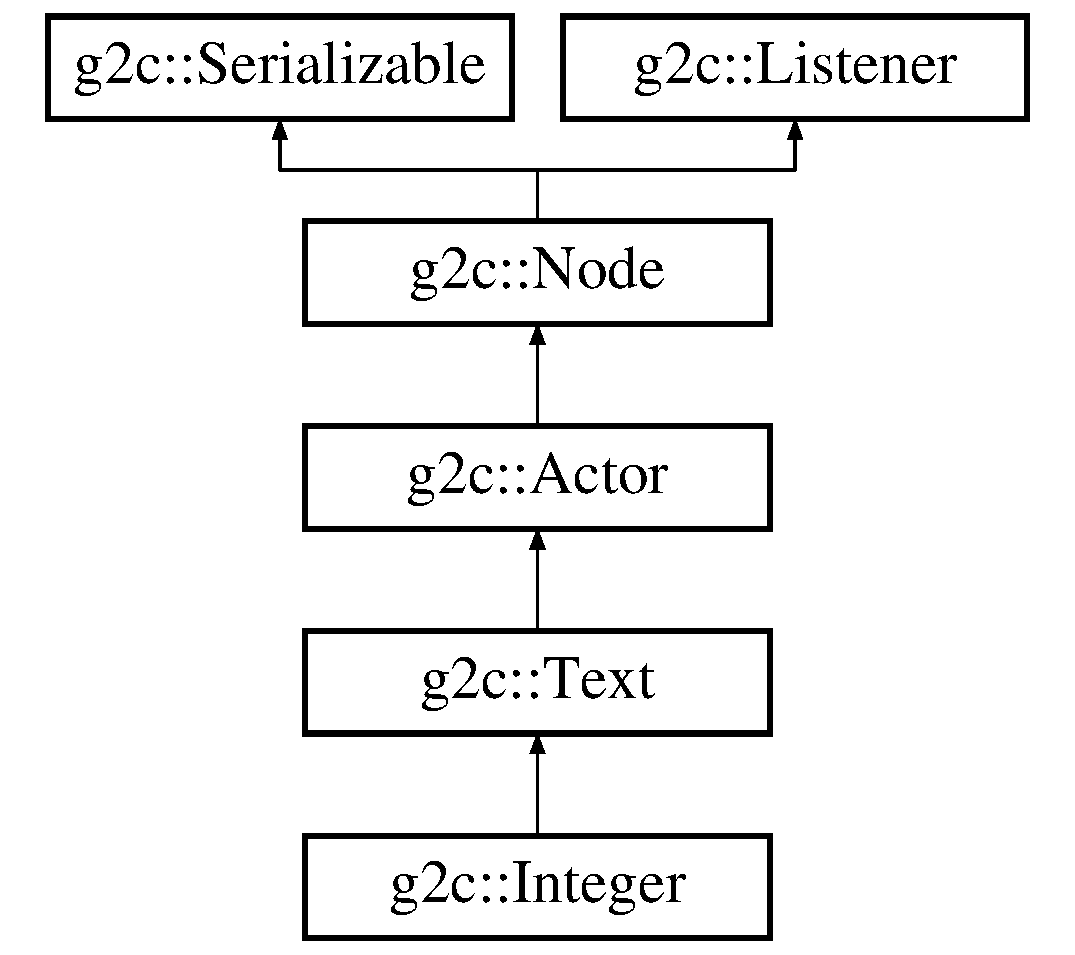
\includegraphics[height=5cm]{classg2c_1_1_integer}
\end{center}
\end{figure}
\subsection*{Public Member Functions}
\begin{DoxyCompactItemize}
\item 
\hypertarget{classg2c_1_1_integer_add9fd9d91de5a9d88f11b5792a46167e}{
{\bfseries Integer} (\hyperlink{classg2c_1_1_font}{Font} $\ast$infont, int $\ast$inptr)}
\label{classg2c_1_1_integer_add9fd9d91de5a9d88f11b5792a46167e}

\item 
virtual void \hyperlink{classg2c_1_1_integer_aac99d7502a55bf5db01f5d673779e36e}{draw} () const 
\end{DoxyCompactItemize}
\subsection*{Public Attributes}
\begin{DoxyCompactItemize}
\item 
\hypertarget{classg2c_1_1_integer_aa7adf2da91c18367bf7da92f7b8a0efb}{
int $\ast$ {\bfseries ptr}}
\label{classg2c_1_1_integer_aa7adf2da91c18367bf7da92f7b8a0efb}

\end{DoxyCompactItemize}


\subsection{Member Function Documentation}
\hypertarget{classg2c_1_1_integer_aac99d7502a55bf5db01f5d673779e36e}{
\index{g2c::Integer@{g2c::Integer}!draw@{draw}}
\index{draw@{draw}!g2c::Integer@{g2c::Integer}}
\subsubsection[{draw}]{\setlength{\rightskip}{0pt plus 5cm}void g2c::Integer::draw () const\hspace{0.3cm}{\ttfamily  \mbox{[}virtual\mbox{]}}}}
\label{classg2c_1_1_integer_aac99d7502a55bf5db01f5d673779e36e}
Draws an image of the c++ string s using the characters in font. 

Reimplemented from \hyperlink{classg2c_1_1_text_ab3296a30652c4c3157ae8a8e87449bb4}{g2c::Text}.

The documentation for this class was generated from the following files:\begin{DoxyCompactItemize}
\item 
sprites.h\item 
sprites.cpp\end{DoxyCompactItemize}

\hypertarget{classg2c_1_1_int_property}{
\section{g2c::IntProperty Class Reference}
\label{classg2c_1_1_int_property}\index{g2c::IntProperty@{g2c::IntProperty}}
}
Inheritance diagram for g2c::IntProperty::\begin{figure}[H]
\begin{center}
\leavevmode
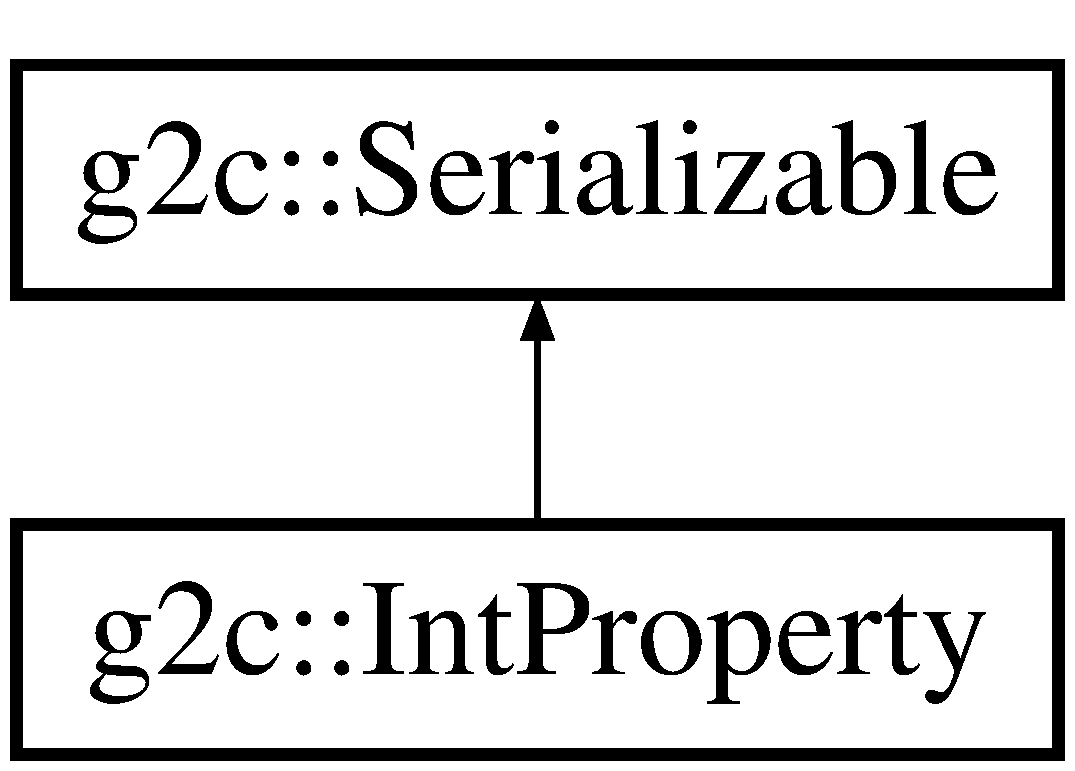
\includegraphics[height=2cm]{classg2c_1_1_int_property}
\end{center}
\end{figure}
\subsection*{Public Member Functions}
\begin{DoxyCompactItemize}
\item 
\hypertarget{classg2c_1_1_int_property_a3af2ffba10f6e60c56ef6c9080371d49}{
{\bfseries IntProperty} (int i)}
\label{classg2c_1_1_int_property_a3af2ffba10f6e60c56ef6c9080371d49}

\item 
\hypertarget{classg2c_1_1_int_property_a246f7e3710103a870e4682d1b204649d}{
virtual std::string {\bfseries serialize} (std::string indent=\char`\"{}\char`\"{}) const }
\label{classg2c_1_1_int_property_a246f7e3710103a870e4682d1b204649d}

\item 
\hypertarget{classg2c_1_1_int_property_a11251ab316b7b728322cf93ae204b960}{
virtual void {\bfseries initWithParseNode} (const \hyperlink{classparse_1_1_node}{parse::Node} $\ast$n)}
\label{classg2c_1_1_int_property_a11251ab316b7b728322cf93ae204b960}

\item 
\hypertarget{classg2c_1_1_int_property_a3eb13d808fee08e98430f18d228f92eb}{
int {\bfseries operator()} () const }
\label{classg2c_1_1_int_property_a3eb13d808fee08e98430f18d228f92eb}

\item 
\hypertarget{classg2c_1_1_int_property_aca77be22b4401b08948dee118ed8985c}{
void {\bfseries operator()} (int i)}
\label{classg2c_1_1_int_property_aca77be22b4401b08948dee118ed8985c}

\item 
\hypertarget{classg2c_1_1_int_property_a1883076bdb55aec9f689a5561cd3ce05}{
bool {\bfseries operator==} (int i) const }
\label{classg2c_1_1_int_property_a1883076bdb55aec9f689a5561cd3ce05}

\item 
\hypertarget{classg2c_1_1_int_property_a1aaa92744d9a4d5ce87395b2cc300c33}{
bool {\bfseries operator!=} (int i) const }
\label{classg2c_1_1_int_property_a1aaa92744d9a4d5ce87395b2cc300c33}

\item 
\hypertarget{classg2c_1_1_int_property_a7cfeacf843766de414635db88bffe771}{
{\bfseries operator int \&} ()}
\label{classg2c_1_1_int_property_a7cfeacf843766de414635db88bffe771}

\item 
\hypertarget{classg2c_1_1_int_property_a15ab7e9edfe7541734e4cdfb2403f0c7}{
{\bfseries operator int const \&} () const }
\label{classg2c_1_1_int_property_a15ab7e9edfe7541734e4cdfb2403f0c7}

\end{DoxyCompactItemize}


The documentation for this class was generated from the following files:\begin{DoxyCompactItemize}
\item 
serializable.h\item 
serializable.cpp\end{DoxyCompactItemize}

\hypertarget{classg2c_1_1_i_o_s_resource_bank}{
\section{g2c::IOSResourceBank Class Reference}
\label{classg2c_1_1_i_o_s_resource_bank}\index{g2c::IOSResourceBank@{g2c::IOSResourceBank}}
}
Inheritance diagram for g2c::IOSResourceBank::\begin{figure}[H]
\begin{center}
\leavevmode
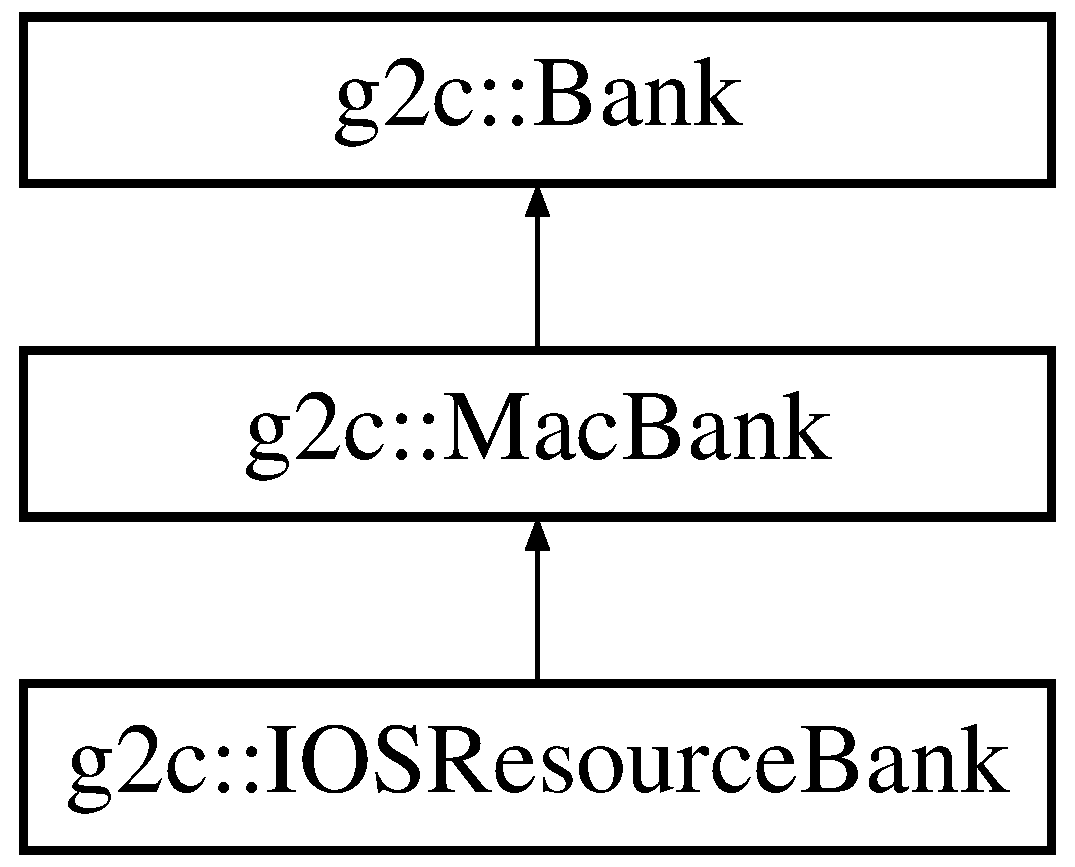
\includegraphics[height=3cm]{classg2c_1_1_i_o_s_resource_bank}
\end{center}
\end{figure}
\subsection*{Public Member Functions}
\begin{DoxyCompactItemize}
\item 
\hypertarget{classg2c_1_1_i_o_s_resource_bank_a32b95b7140db3b44b62c5d006cc2a24c}{
virtual void {\bfseries initPersistentSerializableWithKey} (\hyperlink{classg2c_1_1_serializable}{Serializable} $\ast$s, const char $\ast$key)}
\label{classg2c_1_1_i_o_s_resource_bank_a32b95b7140db3b44b62c5d006cc2a24c}

\item 
\hypertarget{classg2c_1_1_i_o_s_resource_bank_aa451a9ddff750c2fdd3dc7470efb6aac}{
virtual void {\bfseries writePersistentSerializableWithKey} (const \hyperlink{classg2c_1_1_serializable}{Serializable} $\ast$s, const char $\ast$key)}
\label{classg2c_1_1_i_o_s_resource_bank_aa451a9ddff750c2fdd3dc7470efb6aac}

\item 
\hypertarget{classg2c_1_1_i_o_s_resource_bank_a591606485249604a0fe9dda09eb503f0}{
virtual void {\bfseries initSerializableWithPath} (\hyperlink{classg2c_1_1_serializable}{Serializable} $\ast$world, const char $\ast$path)}
\label{classg2c_1_1_i_o_s_resource_bank_a591606485249604a0fe9dda09eb503f0}

\item 
\hypertarget{classg2c_1_1_i_o_s_resource_bank_a4a44fb94323ee11767ec45073bcf4b3f}{
virtual void {\bfseries writeSerializableToPath} (const \hyperlink{classg2c_1_1_serializable}{Serializable} $\ast$world, const char $\ast$path)}
\label{classg2c_1_1_i_o_s_resource_bank_a4a44fb94323ee11767ec45073bcf4b3f}

\item 
\hypertarget{classg2c_1_1_i_o_s_resource_bank_a0dde260f770577f8ec5bfd5244bad8c5}{
virtual void {\bfseries initSoundWithPath} (\hyperlink{classg2c_1_1_sound}{Sound} $\ast$sound, const char $\ast$path)}
\label{classg2c_1_1_i_o_s_resource_bank_a0dde260f770577f8ec5bfd5244bad8c5}

\item 
\hypertarget{classg2c_1_1_i_o_s_resource_bank_a84a7250a86bf2cd643ff5cf7cec52c3e}{
virtual void {\bfseries initBitmapWithPath} (\hyperlink{classg2c_1_1_bitmap}{Bitmap} $\ast$bitmap, const char $\ast$path)}
\label{classg2c_1_1_i_o_s_resource_bank_a84a7250a86bf2cd643ff5cf7cec52c3e}

\end{DoxyCompactItemize}
\subsection*{Public Attributes}
\begin{DoxyCompactItemize}
\item 
\hypertarget{classg2c_1_1_i_o_s_resource_bank_ae72f57b548bb4588241ddc9952693fa1}{
EAGLView $\ast$ {\bfseries view}}
\label{classg2c_1_1_i_o_s_resource_bank_ae72f57b548bb4588241ddc9952693fa1}

\end{DoxyCompactItemize}


The documentation for this class was generated from the following files:\begin{DoxyCompactItemize}
\item 
iosresourcebank.h\item 
iosresourcebank.mm\end{DoxyCompactItemize}

\hypertarget{classg2c_1_1_layer}{
\section{g2c::Layer Class Reference}
\label{classg2c_1_1_layer}\index{g2c::Layer@{g2c::Layer}}
}
Inheritance diagram for g2c::Layer::\begin{figure}[H]
\begin{center}
\leavevmode
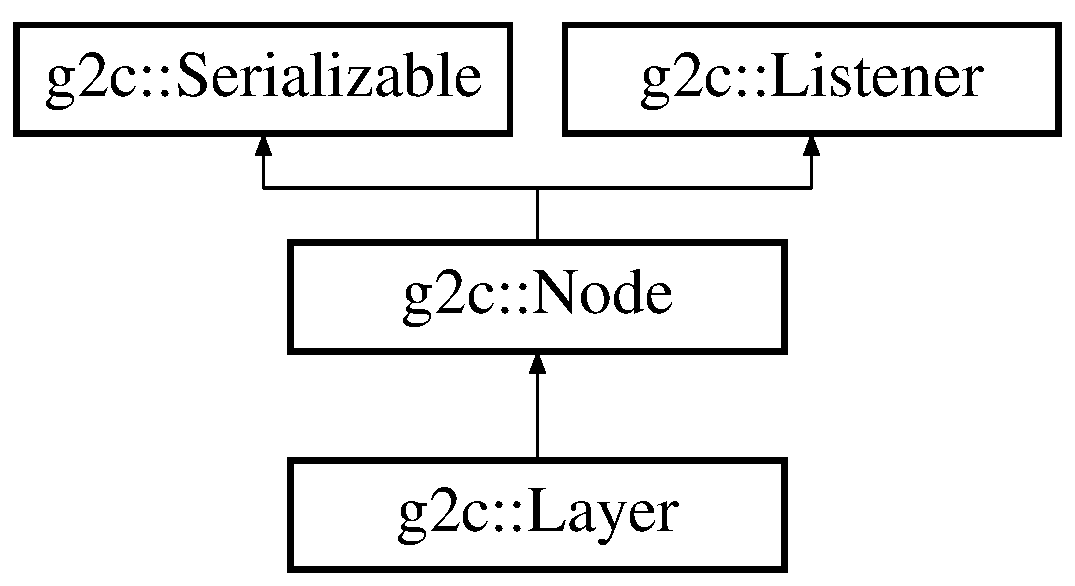
\includegraphics[height=3cm]{classg2c_1_1_layer}
\end{center}
\end{figure}


The documentation for this class was generated from the following files:\begin{DoxyCompactItemize}
\item 
sprites.h\item 
sprites.cpp\end{DoxyCompactItemize}

\hypertarget{classg2c_1_1_listener}{
\section{g2c::Listener Class Reference}
\label{classg2c_1_1_listener}\index{g2c::Listener@{g2c::Listener}}
}
Inheritance diagram for g2c::Listener::\begin{figure}[H]
\begin{center}
\leavevmode
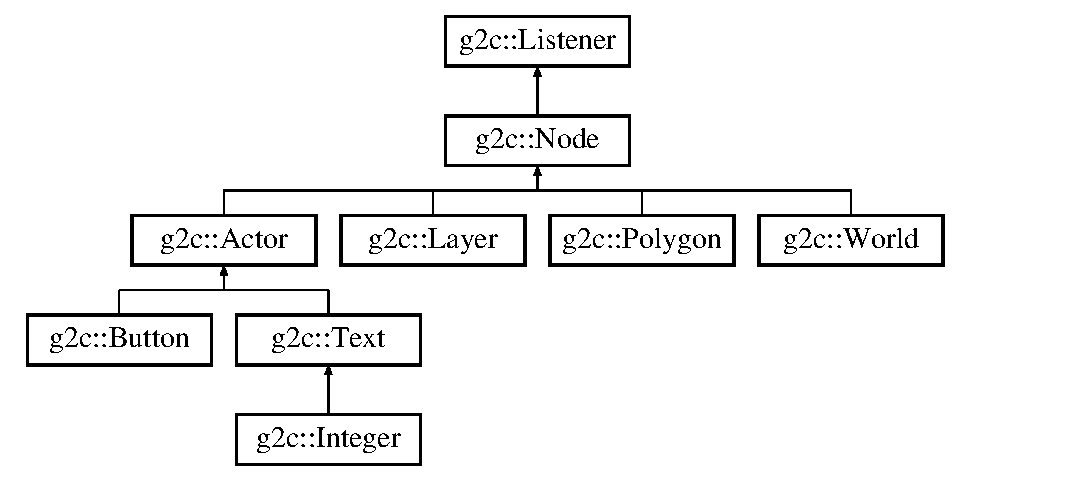
\includegraphics[height=5cm]{classg2c_1_1_listener}
\end{center}
\end{figure}
\subsection*{Public Member Functions}
\begin{DoxyCompactItemize}
\item 
\hypertarget{classg2c_1_1_listener_a2b8deaae3e27f36501bae72316c4fe5c}{
virtual void {\bfseries button} (int b, int state, int x, int y)}
\label{classg2c_1_1_listener_a2b8deaae3e27f36501bae72316c4fe5c}

\item 
\hypertarget{classg2c_1_1_listener_a695fe884b88bb4afcad41802c55ca49e}{
virtual void {\bfseries motion} (int x, int y)}
\label{classg2c_1_1_listener_a695fe884b88bb4afcad41802c55ca49e}

\item 
\hypertarget{classg2c_1_1_listener_a82db635c29eb103d54b2d6ac1fb54389}{
virtual void {\bfseries keyboard} (unsigned char inkey)}
\label{classg2c_1_1_listener_a82db635c29eb103d54b2d6ac1fb54389}

\item 
\hypertarget{classg2c_1_1_listener_a97fe3ed3dd652d7baa239f820f7719f1}{
virtual void {\bfseries keyDown} (unsigned char inkey)}
\label{classg2c_1_1_listener_a97fe3ed3dd652d7baa239f820f7719f1}

\item 
\hypertarget{classg2c_1_1_listener_a96ca8c3605e864048cd96211aec3f69e}{
virtual void {\bfseries keyUp} (unsigned char inkey)}
\label{classg2c_1_1_listener_a96ca8c3605e864048cd96211aec3f69e}

\item 
\hypertarget{classg2c_1_1_listener_ad8a5887401ecfe2b0e4c060e86cf103b}{
virtual void {\bfseries special} (int inkey)}
\label{classg2c_1_1_listener_ad8a5887401ecfe2b0e4c060e86cf103b}

\item 
\hypertarget{classg2c_1_1_listener_a9a7c4697f273982b42f9975787ffb573}{
virtual bool {\bfseries mouseDown} (const Vec2 \&C)}
\label{classg2c_1_1_listener_a9a7c4697f273982b42f9975787ffb573}

\item 
\hypertarget{classg2c_1_1_listener_a581f3f2111d62e9e05ddeb8e731b6373}{
virtual void {\bfseries mouseDragged} (const Vec2 \&C)}
\label{classg2c_1_1_listener_a581f3f2111d62e9e05ddeb8e731b6373}

\item 
\hypertarget{classg2c_1_1_listener_aeb3f29741fb750b8ea2487ec6f018f41}{
virtual void {\bfseries mouseUp} (const Vec2 \&C)}
\label{classg2c_1_1_listener_aeb3f29741fb750b8ea2487ec6f018f41}

\end{DoxyCompactItemize}
\subsection*{Public Attributes}
\begin{DoxyCompactItemize}
\item 
\hypertarget{classg2c_1_1_listener_aa605575ed8d272655e618be0f8463675}{
bool {\bfseries listening}}
\label{classg2c_1_1_listener_aa605575ed8d272655e618be0f8463675}

\item 
\hypertarget{classg2c_1_1_listener_aaea6e353d83b25ed0b7673ef0406fea5}{
\hyperlink{classg2c_1_1_listener}{Listener} $\ast$ {\bfseries delegate}}
\label{classg2c_1_1_listener_aaea6e353d83b25ed0b7673ef0406fea5}

\end{DoxyCompactItemize}
\subsection*{Friends}
\begin{DoxyCompactItemize}
\item 
\hypertarget{classg2c_1_1_listener_aa55d6a52cb291992faebd7b17f6acbcb}{
void {\bfseries fbutton} (int b, int state, int x, int y)}
\label{classg2c_1_1_listener_aa55d6a52cb291992faebd7b17f6acbcb}

\item 
\hypertarget{classg2c_1_1_listener_a92301e62a12c669be2d2c795276d6281}{
void {\bfseries fkeyboard} (unsigned char inkey, int x, int y)}
\label{classg2c_1_1_listener_a92301e62a12c669be2d2c795276d6281}

\item 
\hypertarget{classg2c_1_1_listener_a0aae4450276dc799a287d620b5ef764f}{
void {\bfseries fkeyboardUp} (unsigned char inkey, int x, int y)}
\label{classg2c_1_1_listener_a0aae4450276dc799a287d620b5ef764f}

\item 
\hypertarget{classg2c_1_1_listener_ac92c967f282d0643e4dbe6421a7cc7d3}{
void {\bfseries fspecial} (int inkey, int x, int y)}
\label{classg2c_1_1_listener_ac92c967f282d0643e4dbe6421a7cc7d3}

\item 
\hypertarget{classg2c_1_1_listener_a1754b0ecd84c8a61804a58297e6deb61}{
void {\bfseries fmotion} (int x, int y)}
\label{classg2c_1_1_listener_a1754b0ecd84c8a61804a58297e6deb61}

\end{DoxyCompactItemize}


The documentation for this class was generated from the following files:\begin{DoxyCompactItemize}
\item 
listener.h\item 
listener.cpp\end{DoxyCompactItemize}

\hypertarget{structg2c_1_1_asynchronous_bank_1_1_load_instruction}{
\section{g2c::AsynchronousBank::LoadInstruction Struct Reference}
\label{structg2c_1_1_asynchronous_bank_1_1_load_instruction}\index{g2c::AsynchronousBank::LoadInstruction@{g2c::AsynchronousBank::LoadInstruction}}
}
\subsection*{Public Member Functions}
\begin{DoxyCompactItemize}
\item 
\hypertarget{structg2c_1_1_asynchronous_bank_1_1_load_instruction_a4b07499ca3d50b10da1dae566e562bb4}{
{\bfseries LoadInstruction} (\hyperlink{classg2c_1_1_serializable}{Serializable} $\ast$resource, const std::string \&path)}
\label{structg2c_1_1_asynchronous_bank_1_1_load_instruction_a4b07499ca3d50b10da1dae566e562bb4}

\end{DoxyCompactItemize}
\subsection*{Public Attributes}
\begin{DoxyCompactItemize}
\item 
\hypertarget{structg2c_1_1_asynchronous_bank_1_1_load_instruction_abb990de229ccf5ea6d7f4cdae64230dc}{
\hyperlink{classg2c_1_1_serializable}{Serializable} $\ast$ {\bfseries resource}}
\label{structg2c_1_1_asynchronous_bank_1_1_load_instruction_abb990de229ccf5ea6d7f4cdae64230dc}

\item 
\hypertarget{structg2c_1_1_asynchronous_bank_1_1_load_instruction_a90dc92582af44fcee3f513adf8176053}{
std::string {\bfseries path}}
\label{structg2c_1_1_asynchronous_bank_1_1_load_instruction_a90dc92582af44fcee3f513adf8176053}

\end{DoxyCompactItemize}


The documentation for this struct was generated from the following file:\begin{DoxyCompactItemize}
\item 
bank.h\end{DoxyCompactItemize}

\hypertarget{classg2c_1_1_mac_bank}{
\section{g2c::MacBank Class Reference}
\label{classg2c_1_1_mac_bank}\index{g2c::MacBank@{g2c::MacBank}}
}
Inheritance diagram for g2c::MacBank::\begin{figure}[H]
\begin{center}
\leavevmode
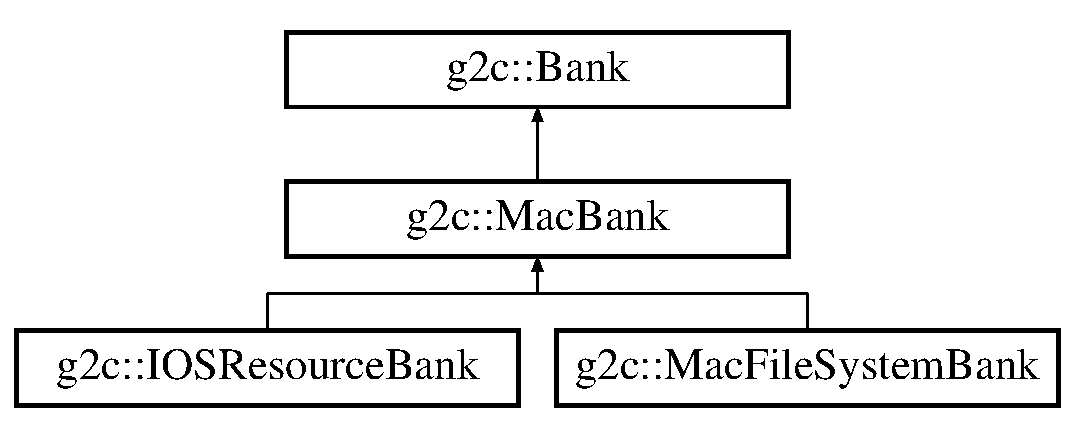
\includegraphics[height=3cm]{classg2c_1_1_mac_bank}
\end{center}
\end{figure}
\subsection*{Public Member Functions}
\begin{DoxyCompactItemize}
\item 
\hypertarget{classg2c_1_1_mac_bank_ad5db791743a30e7d2a82ac585c053eb5}{
virtual void {\bfseries initDataWithPath} (\hyperlink{classg2c_1_1_data}{Data} $\ast$data, const char $\ast$path)}
\label{classg2c_1_1_mac_bank_ad5db791743a30e7d2a82ac585c053eb5}

\item 
\hypertarget{classg2c_1_1_mac_bank_a2432781fb7eab72f72da1a12c9ac6f34}{
virtual void {\bfseries initPersistentSerializableWithKey} (\hyperlink{classg2c_1_1_serializable}{Serializable} $\ast$s, const char $\ast$key)}
\label{classg2c_1_1_mac_bank_a2432781fb7eab72f72da1a12c9ac6f34}

\item 
\hypertarget{classg2c_1_1_mac_bank_aba4c0168c570a4e9ae53a63b71285895}{
virtual void {\bfseries writePersistentSerializableWithKey} (const \hyperlink{classg2c_1_1_serializable}{Serializable} $\ast$s, const char $\ast$key)}
\label{classg2c_1_1_mac_bank_aba4c0168c570a4e9ae53a63b71285895}

\item 
\hypertarget{classg2c_1_1_mac_bank_a5d99c78e0394b7b1ddf9c3e0e6fae06d}{
virtual void {\bfseries initSerializableWithPath} (\hyperlink{classg2c_1_1_serializable}{Serializable} $\ast$s, const char $\ast$path)}
\label{classg2c_1_1_mac_bank_a5d99c78e0394b7b1ddf9c3e0e6fae06d}

\item 
\hypertarget{classg2c_1_1_mac_bank_aa413ee0530ef972b84d583520b12f8d7}{
virtual void {\bfseries writeSerializableToPath} (const \hyperlink{classg2c_1_1_serializable}{Serializable} $\ast$s, const char $\ast$path)}
\label{classg2c_1_1_mac_bank_aa413ee0530ef972b84d583520b12f8d7}

\item 
\hypertarget{classg2c_1_1_mac_bank_aa9091012006c18ada89c0271b2f16bed}{
virtual void {\bfseries initTextureWithPath} (\hyperlink{classg2c_1_1_texture2_d}{Texture2D} $\ast$texture, const char $\ast$path)}
\label{classg2c_1_1_mac_bank_aa9091012006c18ada89c0271b2f16bed}

\item 
\hypertarget{classg2c_1_1_mac_bank_a3d43d417db99484f03e091fc1e378160}{
virtual void {\bfseries initSoundWithPath} (\hyperlink{classg2c_1_1_sound}{Sound} $\ast$sound, const char $\ast$path)}
\label{classg2c_1_1_mac_bank_a3d43d417db99484f03e091fc1e378160}

\item 
\hypertarget{classg2c_1_1_mac_bank_a8a934716f7bfdc914fd42bcf48a2c17a}{
void $\ast$ {\bfseries getOpenALAudioData} (CFURLRef inFileURL, ALsizei $\ast$outDataSize, ALenum $\ast$outDataFormat, ALsizei $\ast$outSampleRate) const }
\label{classg2c_1_1_mac_bank_a8a934716f7bfdc914fd42bcf48a2c17a}

\end{DoxyCompactItemize}
\subsection*{Public Attributes}
\begin{DoxyCompactItemize}
\item 
\hypertarget{classg2c_1_1_mac_bank_a5467056dbe3fa7e7cd93970d198108fd}{
std::string {\bfseries base\_\-path}}
\label{classg2c_1_1_mac_bank_a5467056dbe3fa7e7cd93970d198108fd}

\end{DoxyCompactItemize}
\subsection*{Protected Member Functions}
\begin{DoxyCompactItemize}
\item 
\hypertarget{classg2c_1_1_mac_bank_a066c0d039d054b9f7bf652f20bce36b6}{
void {\bfseries initTextureWithCGImage} (\hyperlink{classg2c_1_1_texture2_d}{Texture2D} $\ast$texture, CGImageRef image)}
\label{classg2c_1_1_mac_bank_a066c0d039d054b9f7bf652f20bce36b6}

\item 
\hypertarget{classg2c_1_1_mac_bank_afc190c0f676881a3f09cd739ac899493}{
void {\bfseries initBitmapWithCGImage} (\hyperlink{classg2c_1_1_bitmap}{Bitmap} $\ast$bitmap, CGImageRef image)}
\label{classg2c_1_1_mac_bank_afc190c0f676881a3f09cd739ac899493}

\end{DoxyCompactItemize}
\subsection*{Protected Attributes}
\begin{DoxyCompactItemize}
\item 
\hypertarget{classg2c_1_1_mac_bank_aa0f97bf47c1c902c060893ec7fad8262}{
std::string {\bfseries directory}}
\label{classg2c_1_1_mac_bank_aa0f97bf47c1c902c060893ec7fad8262}

\end{DoxyCompactItemize}


The documentation for this class was generated from the following files:\begin{DoxyCompactItemize}
\item 
macbank.h\item 
macbank.cpp\end{DoxyCompactItemize}

\hypertarget{classg2c_1_1_mac_file_system_bank}{
\section{g2c::MacFileSystemBank Class Reference}
\label{classg2c_1_1_mac_file_system_bank}\index{g2c::MacFileSystemBank@{g2c::MacFileSystemBank}}
}
Inheritance diagram for g2c::MacFileSystemBank::\begin{figure}[H]
\begin{center}
\leavevmode
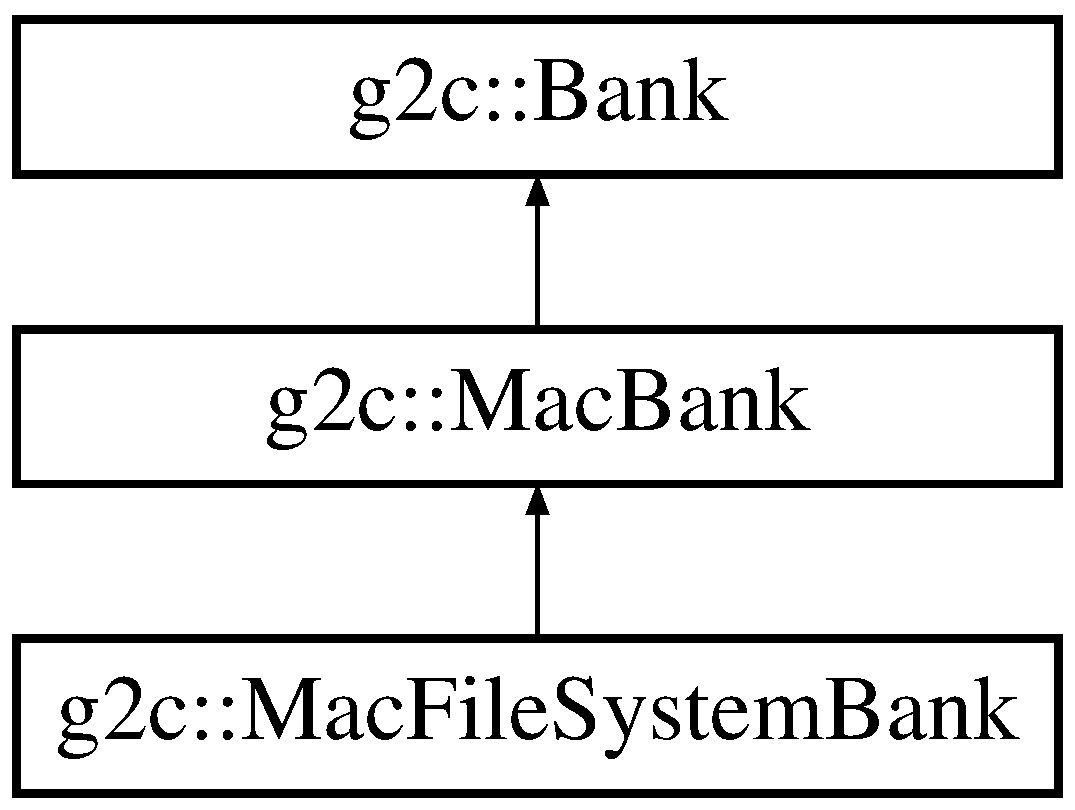
\includegraphics[height=3cm]{classg2c_1_1_mac_file_system_bank}
\end{center}
\end{figure}
\subsection*{Public Member Functions}
\begin{DoxyCompactItemize}
\item 
\hypertarget{classg2c_1_1_mac_file_system_bank_ae55938e2b57d7e89dae2e158aecf66c2}{
virtual void {\bfseries initBitmapWithPath} (\hyperlink{classg2c_1_1_bitmap}{Bitmap} $\ast$bitmap, const char $\ast$path)}
\label{classg2c_1_1_mac_file_system_bank_ae55938e2b57d7e89dae2e158aecf66c2}

\end{DoxyCompactItemize}


The documentation for this class was generated from the following files:\begin{DoxyCompactItemize}
\item 
macbank.h\item 
macbank.cpp\end{DoxyCompactItemize}

\hypertarget{classg2c_1_1_mat4_property}{
\section{g2c::Mat4Property Class Reference}
\label{classg2c_1_1_mat4_property}\index{g2c::Mat4Property@{g2c::Mat4Property}}
}
Inheritance diagram for g2c::Mat4Property::\begin{figure}[H]
\begin{center}
\leavevmode
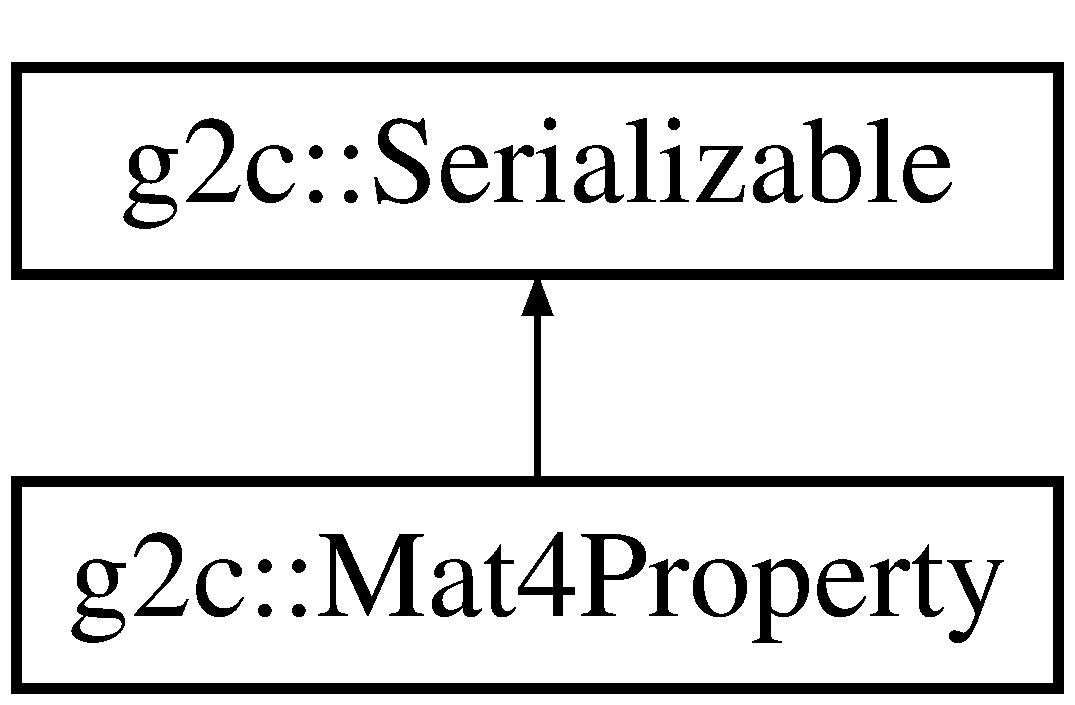
\includegraphics[height=2cm]{classg2c_1_1_mat4_property}
\end{center}
\end{figure}
\subsection*{Public Member Functions}
\begin{DoxyCompactItemize}
\item 
\hypertarget{classg2c_1_1_mat4_property_a8ad71c6bde5b9e3859895cf64e147d42}{
{\bfseries Mat4Property} (const Mat4 \&m)}
\label{classg2c_1_1_mat4_property_a8ad71c6bde5b9e3859895cf64e147d42}

\item 
\hypertarget{classg2c_1_1_mat4_property_ae9b7ef379474f3bd0d19c147e071d069}{
virtual std::string {\bfseries serialize} (std::string indent) const }
\label{classg2c_1_1_mat4_property_ae9b7ef379474f3bd0d19c147e071d069}

\item 
\hypertarget{classg2c_1_1_mat4_property_a8e1515986b4345c1341a2b486fc6e688}{
void {\bfseries initWithParseNode} (const \hyperlink{classparse_1_1_node}{parse::Node} $\ast$n)}
\label{classg2c_1_1_mat4_property_a8e1515986b4345c1341a2b486fc6e688}

\end{DoxyCompactItemize}


The documentation for this class was generated from the following files:\begin{DoxyCompactItemize}
\item 
sprites.h\item 
sprites.cpp\end{DoxyCompactItemize}

\hypertarget{classg2c_1_1_mesh}{
\section{g2c::Mesh Class Reference}
\label{classg2c_1_1_mesh}\index{g2c::Mesh@{g2c::Mesh}}
}


{\ttfamily \#include $<$sprites.h$>$}\subsection*{Public Types}
\begin{DoxyCompactItemize}
\item 
enum {\bfseries ElementType} \{ {\bfseries kTriangles}, 
{\bfseries kLines}
 \}
\end{DoxyCompactItemize}
\subsection*{Public Member Functions}
\begin{DoxyCompactItemize}
\item 
\hypertarget{classg2c_1_1_mesh_a7c28bc8c50be706d83c6e20804c2d695}{
void {\bfseries resize} (int inNumberOfVertices, int inNumberOfElements)}
\label{classg2c_1_1_mesh_a7c28bc8c50be706d83c6e20804c2d695}

\end{DoxyCompactItemize}
\subsection*{Public Attributes}
\begin{DoxyCompactItemize}
\item 
\hypertarget{classg2c_1_1_mesh_a2d68f79ca34f6a4fb8d6906e696309c2}{
int {\bfseries numberOfVertices}}
\label{classg2c_1_1_mesh_a2d68f79ca34f6a4fb8d6906e696309c2}

\item 
\hypertarget{classg2c_1_1_mesh_a6bb9fc24ca1c81bdb1c55ca59e33a8b5}{
int {\bfseries numberOfElements}}
\label{classg2c_1_1_mesh_a6bb9fc24ca1c81bdb1c55ca59e33a8b5}

\item 
\hypertarget{classg2c_1_1_mesh_a3535f7f7fe763e7958a2eb9dcadf37ff}{
ElementType {\bfseries elementType}}
\label{classg2c_1_1_mesh_a3535f7f7fe763e7958a2eb9dcadf37ff}

\item 
\hypertarget{classg2c_1_1_mesh_a02fe24297627cf19d4fb73e89753c9ea}{
float $\ast$ {\bfseries positions}}
\label{classg2c_1_1_mesh_a02fe24297627cf19d4fb73e89753c9ea}

\item 
\hypertarget{classg2c_1_1_mesh_a7ad3d1f591acca69de3df482523856ab}{
short $\ast$ {\bfseries indices}}
\label{classg2c_1_1_mesh_a7ad3d1f591acca69de3df482523856ab}

\end{DoxyCompactItemize}


\subsection{Detailed Description}
\hyperlink{classg2c_1_1_mesh}{Mesh} represents a collection of planar triangles or line segments to be drawn on the screen. To draw a mesh, populate positions and vertices 

The documentation for this class was generated from the following files:\begin{DoxyCompactItemize}
\item 
sprites.h\item 
sprites.cpp\end{DoxyCompactItemize}

\hypertarget{classg2c_1_1_model}{
\section{g2c::Model Class Reference}
\label{classg2c_1_1_model}\index{g2c::Model@{g2c::Model}}
}
Inheritance diagram for g2c::Model::\begin{figure}[H]
\begin{center}
\leavevmode
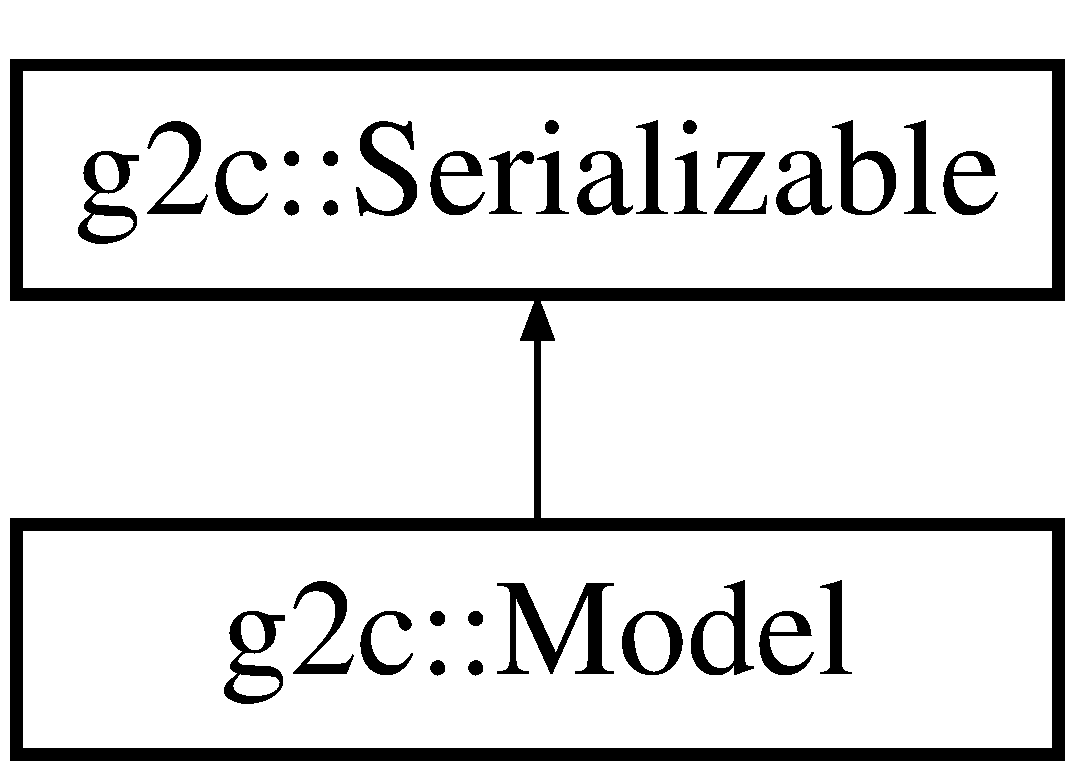
\includegraphics[height=2cm]{classg2c_1_1_model}
\end{center}
\end{figure}
\subsection*{Public Member Functions}
\begin{DoxyCompactItemize}
\item 
\hypertarget{classg2c_1_1_model_ad03aaa5728a9fdf16857b914c30e8424}{
void {\bfseries draw} () const }
\label{classg2c_1_1_model_ad03aaa5728a9fdf16857b914c30e8424}

\item 
\hypertarget{classg2c_1_1_model_a413d5a406612ebf4bc196f5830d33fa7}{
\hyperlink{classg2c_1_1_model}{Model} \& {\bfseries add} (\hyperlink{classg2c_1_1_element}{Element} $\ast$element, bool flagForDelete=false)}
\label{classg2c_1_1_model_a413d5a406612ebf4bc196f5830d33fa7}

\item 
\hypertarget{classg2c_1_1_model_a61713fda8fabb7417fb3907715a17819}{
\hyperlink{classg2c_1_1_model}{Model} \& {\bfseries add} (const \hyperlink{classg2c_1_1_model}{Model} \&element, bool flagForDelete=false)}
\label{classg2c_1_1_model_a61713fda8fabb7417fb3907715a17819}

\item 
\hypertarget{classg2c_1_1_model_a8a2dfbe528f8db727a16355645d0fef4}{
void {\bfseries makeMaps} ()}
\label{classg2c_1_1_model_a8a2dfbe528f8db727a16355645d0fef4}

\item 
\hypertarget{classg2c_1_1_model_a46e2e03ebb2b4c1f9beb0fd2286628be}{
void {\bfseries compileEffects} ()}
\label{classg2c_1_1_model_a46e2e03ebb2b4c1f9beb0fd2286628be}

\item 
\hypertarget{classg2c_1_1_model_af1a5e483a08dd2d25fc3f8f7aa27e178}{
void {\bfseries resolveNames} ()}
\label{classg2c_1_1_model_af1a5e483a08dd2d25fc3f8f7aa27e178}

\end{DoxyCompactItemize}
\subsection*{Public Attributes}
\begin{DoxyCompactItemize}
\item 
\hypertarget{classg2c_1_1_model_aede46e88355f5b55c4088e0bf01e8744}{
\hyperlink{classg2c_1_1_bank}{Bank} $\ast$ {\bfseries bank}}
\label{classg2c_1_1_model_aede46e88355f5b55c4088e0bf01e8744}

\item 
\hypertarget{classg2c_1_1_model_a9228ed89466cb94aea226300ccc2f19c}{
std::vector$<$ std::string $>$ {\bfseries include}}
\label{classg2c_1_1_model_a9228ed89466cb94aea226300ccc2f19c}

\item 
\hypertarget{classg2c_1_1_model_a149b71f7012c169a11a5c451ab29c8d9}{
std::map$<$ std::string, \hyperlink{classg2c_1_1_texture}{Texture} $\ast$ $>$ {\bfseries textures}}
\label{classg2c_1_1_model_a149b71f7012c169a11a5c451ab29c8d9}

\item 
\hypertarget{classg2c_1_1_model_a35248d5aae947c5ee4d728b6dfb077b2}{
std::map$<$ std::string, \hyperlink{classg2c_1_1_assumption}{Assumption} $\ast$ $>$ {\bfseries assumptions}}
\label{classg2c_1_1_model_a35248d5aae947c5ee4d728b6dfb077b2}

\item 
\hypertarget{classg2c_1_1_model_ab845bca67dea602b512d6a82b6c4bca0}{
std::map$<$ std::string, \hyperlink{classg2c_1_1_effect}{Effect} $\ast$ $>$ {\bfseries effects}}
\label{classg2c_1_1_model_ab845bca67dea602b512d6a82b6c4bca0}

\item 
\hypertarget{classg2c_1_1_model_a8c4c0aae735564dc4d2c6c73ead144a8}{
std::map$<$ std::string, \hyperlink{classg2c_1_1_buffer}{Buffer} $\ast$ $>$ {\bfseries buffers}}
\label{classg2c_1_1_model_a8c4c0aae735564dc4d2c6c73ead144a8}

\item 
\hypertarget{classg2c_1_1_model_a1d2402bab3cd380753e71f44a3a6e564}{
std::map$<$ std::string, \hyperlink{classg2c_1_1_index_buffer}{IndexBuffer} $\ast$ $>$ {\bfseries indexBuffers}}
\label{classg2c_1_1_model_a1d2402bab3cd380753e71f44a3a6e564}

\item 
\hypertarget{classg2c_1_1_model_a76e1514935ee35ff6ea820fa7b0410b3}{
std::map$<$ std::string, \hyperlink{classg2c_1_1_geometry}{Geometry} $\ast$ $>$ {\bfseries geometries}}
\label{classg2c_1_1_model_a76e1514935ee35ff6ea820fa7b0410b3}

\item 
\hypertarget{classg2c_1_1_model_afcb536300e2316f23d960e8301e09199}{
std::map$<$ std::string, \hyperlink{classg2c_1_1_shape}{Shape} $\ast$ $>$ {\bfseries shapes}}
\label{classg2c_1_1_model_afcb536300e2316f23d960e8301e09199}

\end{DoxyCompactItemize}
\subsection*{Protected Member Functions}
\begin{DoxyCompactItemize}
\item 
\hypertarget{classg2c_1_1_model_a4992a4fc88bb1595e1ad85ea9a31a7bd}{
virtual std::string {\bfseries serializeElements} (std::string indent=\char`\"{}\char`\"{}) const }
\label{classg2c_1_1_model_a4992a4fc88bb1595e1ad85ea9a31a7bd}

\item 
\hypertarget{classg2c_1_1_model_ae527cab9ea535e4cae434afd25cd80e6}{
virtual void {\bfseries deserialize} (const std::string \&s)}
\label{classg2c_1_1_model_ae527cab9ea535e4cae434afd25cd80e6}

\item 
\hypertarget{classg2c_1_1_model_ae3ff150b2ff56b6e6413972524a20dee}{
virtual void {\bfseries handleChild} (const \hyperlink{classparse_1_1_node}{parse::Node} $\ast$n)}
\label{classg2c_1_1_model_ae3ff150b2ff56b6e6413972524a20dee}

\end{DoxyCompactItemize}
\subsection*{Protected Attributes}
\begin{DoxyCompactItemize}
\item 
\hypertarget{classg2c_1_1_model_afd27c177f46e2e4ca39d2de58f564ca5}{
std::set$<$ \hyperlink{classg2c_1_1_element}{Element} $\ast$ $>$ {\bfseries deleteMe}}
\label{classg2c_1_1_model_afd27c177f46e2e4ca39d2de58f564ca5}

\item 
\hypertarget{classg2c_1_1_model_a3b9a49e442e7d51057413d82256f0451}{
std::vector$<$ \hyperlink{classg2c_1_1_element}{Element} $\ast$ $>$ {\bfseries elements}}
\label{classg2c_1_1_model_a3b9a49e442e7d51057413d82256f0451}

\end{DoxyCompactItemize}
\subsection*{Friends}
\begin{DoxyCompactItemize}
\item 
\hypertarget{classg2c_1_1_model_a016b821f88c7c0a2de1451c175cefbf9}{
class {\bfseries Element}}
\label{classg2c_1_1_model_a016b821f88c7c0a2de1451c175cefbf9}

\item 
\hypertarget{classg2c_1_1_model_aa70951a0328ba29f64176f16b3ea47d8}{
class {\bfseries Texture2D}}
\label{classg2c_1_1_model_aa70951a0328ba29f64176f16b3ea47d8}

\item 
\hypertarget{classg2c_1_1_model_a83d06bada150194666fdc02c043d1080}{
class {\bfseries CubeMap}}
\label{classg2c_1_1_model_a83d06bada150194666fdc02c043d1080}

\item 
\hypertarget{classg2c_1_1_model_ac8649272bb0576cc72f2486439664efe}{
class {\bfseries Effect}}
\label{classg2c_1_1_model_ac8649272bb0576cc72f2486439664efe}

\item 
\hypertarget{classg2c_1_1_model_a6cc942b96f148de5aefd7f1c72801b62}{
class {\bfseries Assumption}}
\label{classg2c_1_1_model_a6cc942b96f148de5aefd7f1c72801b62}

\item 
\hypertarget{classg2c_1_1_model_a9aca7b7350e6ffa0e2d6320834ad1857}{
class {\bfseries Geometry}}
\label{classg2c_1_1_model_a9aca7b7350e6ffa0e2d6320834ad1857}

\item 
\hypertarget{classg2c_1_1_model_a1e1ef8352d0a310bace7f7a3307d1378}{
class {\bfseries Shape}}
\label{classg2c_1_1_model_a1e1ef8352d0a310bace7f7a3307d1378}

\item 
\hypertarget{classg2c_1_1_model_a5ba04a2bf0ca34a0f845cd759950664d}{
class {\bfseries Buffer}}
\label{classg2c_1_1_model_a5ba04a2bf0ca34a0f845cd759950664d}

\item 
\hypertarget{classg2c_1_1_model_a95054ec4e847742ba17d0350fc1fa8fa}{
class {\bfseries IndexBuffer}}
\label{classg2c_1_1_model_a95054ec4e847742ba17d0350fc1fa8fa}

\item 
\hypertarget{classg2c_1_1_model_aaec47a26a3c11c1debd3ed922b69cbd2}{
class {\bfseries Field}}
\label{classg2c_1_1_model_aaec47a26a3c11c1debd3ed922b69cbd2}

\end{DoxyCompactItemize}


The documentation for this class was generated from the following files:\begin{DoxyCompactItemize}
\item 
graphics.h\item 
graphics.cpp\end{DoxyCompactItemize}

\hypertarget{classg2c_1_1_move_matrix}{
\section{g2c::MoveMatrix Class Reference}
\label{classg2c_1_1_move_matrix}\index{g2c::MoveMatrix@{g2c::MoveMatrix}}
}
Inheritance diagram for g2c::MoveMatrix::\begin{figure}[H]
\begin{center}
\leavevmode
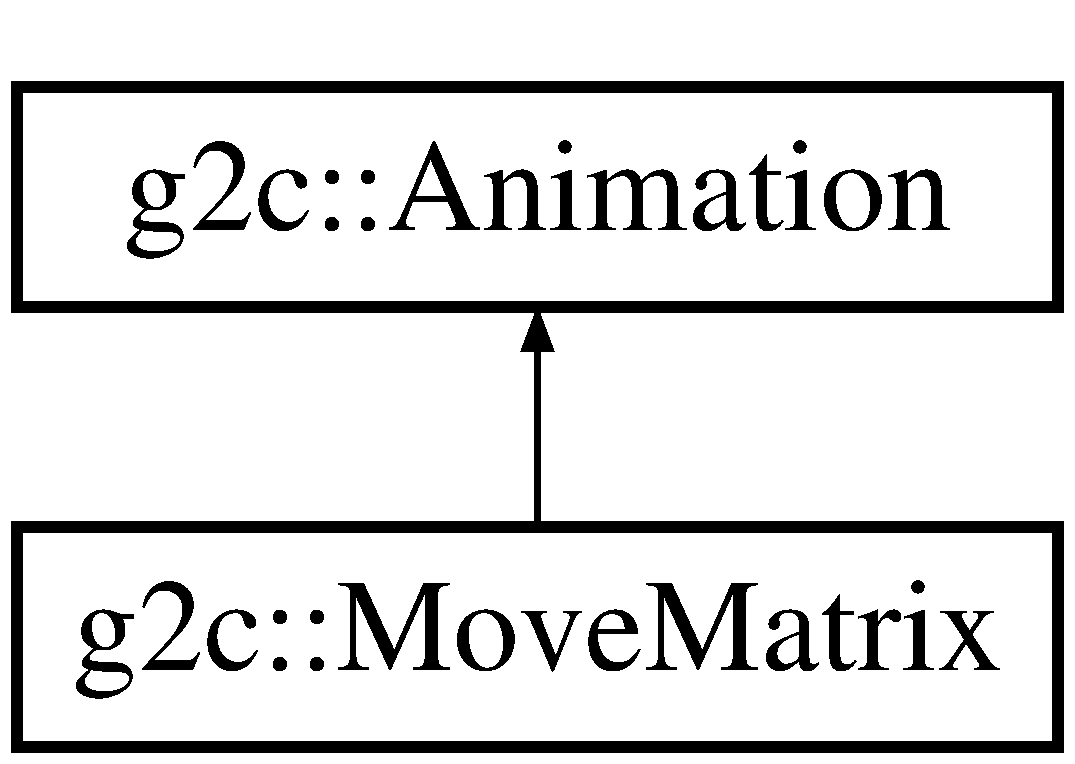
\includegraphics[height=2cm]{classg2c_1_1_move_matrix}
\end{center}
\end{figure}
\subsection*{Public Member Functions}
\begin{DoxyCompactItemize}
\item 
\hypertarget{classg2c_1_1_move_matrix_a6758418174891c8811a5097abddcc9cf}{
{\bfseries MoveMatrix} (double instart, double induration, Mat4 $\ast$inm, const Mat4 \&indst)}
\label{classg2c_1_1_move_matrix_a6758418174891c8811a5097abddcc9cf}

\item 
\hypertarget{classg2c_1_1_move_matrix_ad8adb4906302730891e35cd3ca479ddc}{
virtual void {\bfseries begin} ()}
\label{classg2c_1_1_move_matrix_ad8adb4906302730891e35cd3ca479ddc}

\item 
\hypertarget{classg2c_1_1_move_matrix_a6332271935a779775608173bd2e43d93}{
virtual void {\bfseries step} (double t)}
\label{classg2c_1_1_move_matrix_a6332271935a779775608173bd2e43d93}

\item 
\hypertarget{classg2c_1_1_move_matrix_a317c86c003346c0960333a2b060262be}{
virtual void {\bfseries end} ()}
\label{classg2c_1_1_move_matrix_a317c86c003346c0960333a2b060262be}

\end{DoxyCompactItemize}
\subsection*{Public Attributes}
\begin{DoxyCompactItemize}
\item 
\hypertarget{classg2c_1_1_move_matrix_a0094dfbb7dbfcb12775b4316b64a9c7a}{
Mat4 $\ast$ {\bfseries m}}
\label{classg2c_1_1_move_matrix_a0094dfbb7dbfcb12775b4316b64a9c7a}

\item 
\hypertarget{classg2c_1_1_move_matrix_ae83d9ef3e4a581580693afb965a0d5c7}{
Mat4 {\bfseries src}}
\label{classg2c_1_1_move_matrix_ae83d9ef3e4a581580693afb965a0d5c7}

\item 
\hypertarget{classg2c_1_1_move_matrix_a7b85bd72745ee41a1e41163d795355be}{
Mat4 {\bfseries dst}}
\label{classg2c_1_1_move_matrix_a7b85bd72745ee41a1e41163d795355be}

\end{DoxyCompactItemize}


The documentation for this class was generated from the following files:\begin{DoxyCompactItemize}
\item 
animations.h\item 
animations.cpp\end{DoxyCompactItemize}

\hypertarget{classg2c_1_1_move_vec2}{
\section{g2c::MoveVec2 Class Reference}
\label{classg2c_1_1_move_vec2}\index{g2c::MoveVec2@{g2c::MoveVec2}}
}
Inheritance diagram for g2c::MoveVec2::\begin{figure}[H]
\begin{center}
\leavevmode
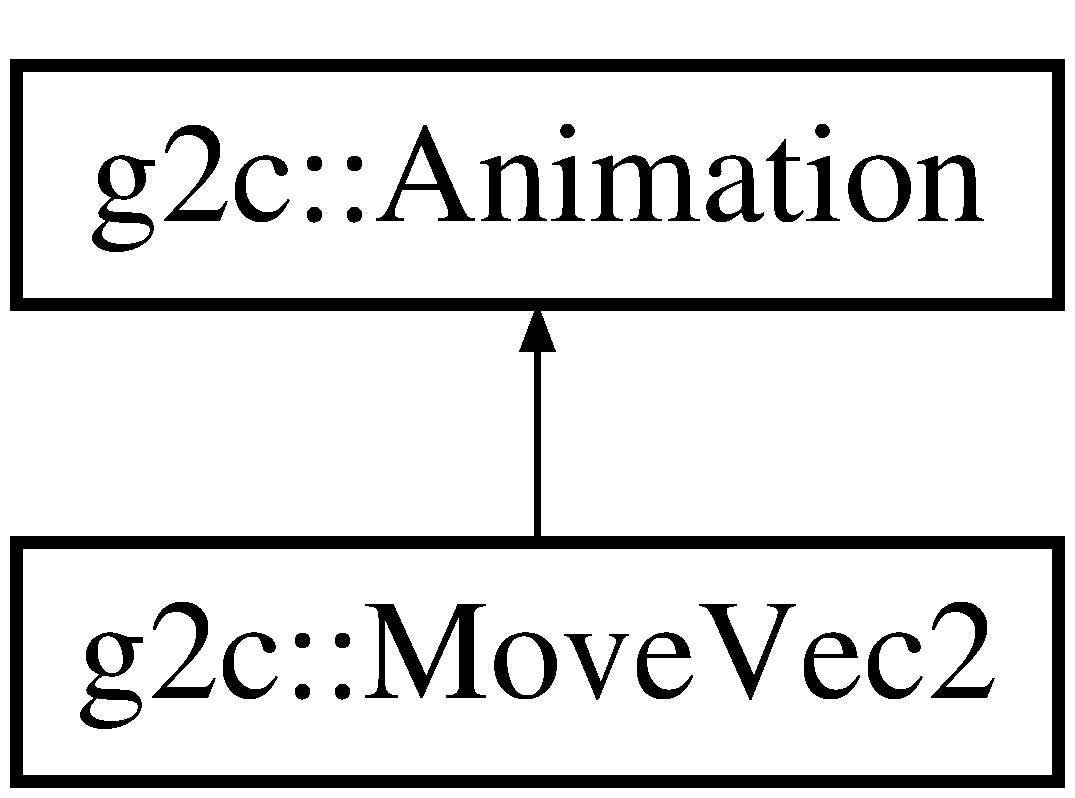
\includegraphics[height=2cm]{classg2c_1_1_move_vec2}
\end{center}
\end{figure}
\subsection*{Public Member Functions}
\begin{DoxyCompactItemize}
\item 
\hypertarget{classg2c_1_1_move_vec2_a48e994e1126cb392be0a85be44d4f360}{
{\bfseries MoveVec2} (double instart, double induration, Vec2 $\ast$inv, const Vec2 \&indst)}
\label{classg2c_1_1_move_vec2_a48e994e1126cb392be0a85be44d4f360}

\item 
\hypertarget{classg2c_1_1_move_vec2_a705bc4f8abd8d37d908ca0a73d92b90c}{
virtual void {\bfseries begin} ()}
\label{classg2c_1_1_move_vec2_a705bc4f8abd8d37d908ca0a73d92b90c}

\item 
\hypertarget{classg2c_1_1_move_vec2_ac1e6597c52356e77bfc951a78e5a5cd1}{
virtual void {\bfseries step} (double t)}
\label{classg2c_1_1_move_vec2_ac1e6597c52356e77bfc951a78e5a5cd1}

\item 
\hypertarget{classg2c_1_1_move_vec2_ae79f50336f80d7155fc3b4c6f577cc85}{
virtual void {\bfseries end} ()}
\label{classg2c_1_1_move_vec2_ae79f50336f80d7155fc3b4c6f577cc85}

\end{DoxyCompactItemize}
\subsection*{Public Attributes}
\begin{DoxyCompactItemize}
\item 
\hypertarget{classg2c_1_1_move_vec2_adffd57ff283ab8f3384cde36eab6b88e}{
Vec2 $\ast$ {\bfseries v}}
\label{classg2c_1_1_move_vec2_adffd57ff283ab8f3384cde36eab6b88e}

\item 
\hypertarget{classg2c_1_1_move_vec2_a9a44968808e5bdf7ba6d62c0f769d8b9}{
Vec2 {\bfseries src}}
\label{classg2c_1_1_move_vec2_a9a44968808e5bdf7ba6d62c0f769d8b9}

\item 
\hypertarget{classg2c_1_1_move_vec2_a36bef88ed8c24fde755fb29e107ddff7}{
Vec2 {\bfseries dst}}
\label{classg2c_1_1_move_vec2_a36bef88ed8c24fde755fb29e107ddff7}

\end{DoxyCompactItemize}


The documentation for this class was generated from the following files:\begin{DoxyCompactItemize}
\item 
animations.h\item 
animations.cpp\end{DoxyCompactItemize}

\hypertarget{classparse_1_1_node}{
\section{parse::Node Class Reference}
\label{classparse_1_1_node}\index{parse::Node@{parse::Node}}
}
\subsection*{Public Member Functions}
\begin{DoxyCompactItemize}
\item 
\hypertarget{classparse_1_1_node_a526b89693b5a6be5debdee9baa346851}{
{\bfseries Node} (const char $\ast$s)}
\label{classparse_1_1_node_a526b89693b5a6be5debdee9baa346851}

\item 
\hypertarget{classparse_1_1_node_a1f16e15ad1eb54eeafe435bc248c9d20}{
{\bfseries Node} (const char $\ast$s, int begin, int end)}
\label{classparse_1_1_node_a1f16e15ad1eb54eeafe435bc248c9d20}

\item 
\hypertarget{classparse_1_1_node_afbf3e1110cda6b2dd7ccc5c0fd3067ea}{
void {\bfseries display} () const }
\label{classparse_1_1_node_afbf3e1110cda6b2dd7ccc5c0fd3067ea}

\item 
\hypertarget{classparse_1_1_node_a391e7163709229848ca02ba5316cf0aa}{
void {\bfseries print} () const }
\label{classparse_1_1_node_a391e7163709229848ca02ba5316cf0aa}

\end{DoxyCompactItemize}
\subsection*{Public Attributes}
\begin{DoxyCompactItemize}
\item 
\hypertarget{classparse_1_1_node_a71b2c8efa3df8dac06ec93aa2890636c}{
const char $\ast$ {\bfseries s}}
\label{classparse_1_1_node_a71b2c8efa3df8dac06ec93aa2890636c}

\item 
\hypertarget{classparse_1_1_node_a61bc6c394e8663082327e3cf7f7b0a8d}{
int {\bfseries begin}}
\label{classparse_1_1_node_a61bc6c394e8663082327e3cf7f7b0a8d}

\item 
\hypertarget{classparse_1_1_node_a5b2c37eaa4fbd9f32a9a91fbb4a95781}{
int {\bfseries end}}
\label{classparse_1_1_node_a5b2c37eaa4fbd9f32a9a91fbb4a95781}

\item 
\hypertarget{classparse_1_1_node_a67c274650ec5dee32067f19a3ff3223a}{
Type {\bfseries type}}
\label{classparse_1_1_node_a67c274650ec5dee32067f19a3ff3223a}

\item 
\hypertarget{classparse_1_1_node_a9bab9e21d3c186688b3169d499ef7af4}{
\hyperlink{classparse_1_1_data}{Data} {\bfseries data}}
\label{classparse_1_1_node_a9bab9e21d3c186688b3169d499ef7af4}

\item 
\hypertarget{classparse_1_1_node_af3c7f22adb4488b70b432907f255e2a4}{
std::vector$<$ \hyperlink{classparse_1_1_node}{Node} $\ast$ $>$ {\bfseries children}}
\label{classparse_1_1_node_af3c7f22adb4488b70b432907f255e2a4}

\end{DoxyCompactItemize}
\subsection*{Protected Member Functions}
\begin{DoxyCompactItemize}
\item 
\hypertarget{classparse_1_1_node_af294665a037deb78fe2a839d8be65fdf}{
void {\bfseries parse} ()}
\label{classparse_1_1_node_af294665a037deb78fe2a839d8be65fdf}

\item 
\hypertarget{classparse_1_1_node_acdfa2f21dea5f671aa653ee607500d99}{
void {\bfseries clearChildren} ()}
\label{classparse_1_1_node_acdfa2f21dea5f671aa653ee607500d99}

\end{DoxyCompactItemize}


The documentation for this class was generated from the following files:\begin{DoxyCompactItemize}
\item 
parse.h\item 
parse.cpp\end{DoxyCompactItemize}

\hypertarget{classg2c_1_1_node}{
\section{g2c::Node Class Reference}
\label{classg2c_1_1_node}\index{g2c::Node@{g2c::Node}}
}


{\ttfamily \#include $<$sprites.h$>$}Inheritance diagram for g2c::Node::\begin{figure}[H]
\begin{center}
\leavevmode
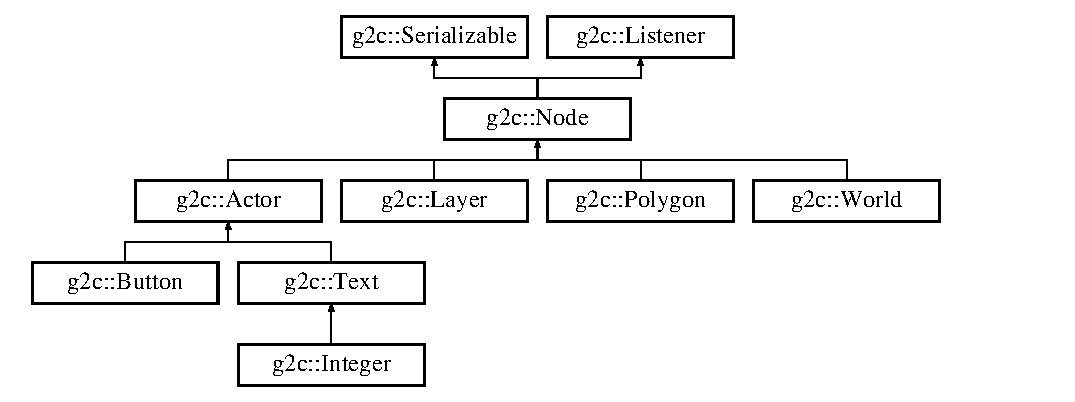
\includegraphics[height=4.95575cm]{classg2c_1_1_node}
\end{center}
\end{figure}
\subsection*{Public Member Functions}
\begin{DoxyCompactItemize}
\item 
\hypertarget{classg2c_1_1_node_aa6d5ce9f6bff259d79c34a6923ab7e18}{
\hyperlink{classg2c_1_1_node}{Node} $\ast$ {\bfseries findChild} (const std::string \&name) const }
\label{classg2c_1_1_node_aa6d5ce9f6bff259d79c34a6923ab7e18}

\item 
\hypertarget{classg2c_1_1_node_a698332ea09f276a296102e1645de3fc4}{
void {\bfseries add} (\hyperlink{classg2c_1_1_node}{Node} $\ast$t)}
\label{classg2c_1_1_node_a698332ea09f276a296102e1645de3fc4}

\item 
\hypertarget{classg2c_1_1_node_af9960ae3bfbb5a116667bb0a1aeffd7f}{
void {\bfseries addAtIndex} (\hyperlink{classg2c_1_1_node}{Node} $\ast$t, int index)}
\label{classg2c_1_1_node_af9960ae3bfbb5a116667bb0a1aeffd7f}

\item 
\hypertarget{classg2c_1_1_node_ae3485a8c3dfb0bd397aff4d283964498}{
int {\bfseries indexOf} (const \hyperlink{classg2c_1_1_node}{Node} $\ast$t) const }
\label{classg2c_1_1_node_ae3485a8c3dfb0bd397aff4d283964498}

\item 
\hypertarget{classg2c_1_1_node_a56f487a49b2221469568ea8587645e51}{
void {\bfseries remove} (\hyperlink{classg2c_1_1_node}{Node} $\ast$t)}
\label{classg2c_1_1_node_a56f487a49b2221469568ea8587645e51}

\item 
\hypertarget{classg2c_1_1_node_a8745619ad7458808da226105aa12d08c}{
void {\bfseries removeAndDelete} (\hyperlink{classg2c_1_1_node}{Node} $\ast$t)}
\label{classg2c_1_1_node_a8745619ad7458808da226105aa12d08c}

\item 
\hypertarget{classg2c_1_1_node_ac660db669518df6974163453edc8cb49}{
virtual void {\bfseries removeSprite} (const \hyperlink{classg2c_1_1_sprite}{Sprite} $\ast$sprite)}
\label{classg2c_1_1_node_ac660db669518df6974163453edc8cb49}

\item 
\hypertarget{classg2c_1_1_node_a138ae78f70f933cbee525f2891b3ab97}{
void {\bfseries clearChildren} ()}
\label{classg2c_1_1_node_a138ae78f70f933cbee525f2891b3ab97}

\item 
\hypertarget{classg2c_1_1_node_a8778eb7b0d15a763a2d08815f92dfadb}{
virtual void {\bfseries draw} () const }
\label{classg2c_1_1_node_a8778eb7b0d15a763a2d08815f92dfadb}

\item 
\hypertarget{classg2c_1_1_node_af161518b302eee61afa0b9a5e96923df}{
virtual \hyperlink{classg2c_1_1_actor}{Actor} $\ast$ {\bfseries actorInClick} (const Vec2 \&C)}
\label{classg2c_1_1_node_af161518b302eee61afa0b9a5e96923df}

\item 
\hypertarget{classg2c_1_1_node_ae14520472896031136193b8976b95bac}{
virtual void {\bfseries handleChild} (const \hyperlink{classparse_1_1_node}{parse::Node} $\ast$n)}
\label{classg2c_1_1_node_ae14520472896031136193b8976b95bac}

\item 
\hypertarget{classg2c_1_1_node_a5b31987b395473e03e7452ec6a2c79ff}{
virtual bool {\bfseries vectorInside} (const Vec2 \&V) const }
\label{classg2c_1_1_node_a5b31987b395473e03e7452ec6a2c79ff}

\item 
\hypertarget{classg2c_1_1_node_a6cffd425eec0487e34656e2508ce16ab}{
virtual void {\bfseries keyboard} (unsigned char inkey)}
\label{classg2c_1_1_node_a6cffd425eec0487e34656e2508ce16ab}

\item 
\hypertarget{classg2c_1_1_node_ab60d344a72277e988af8ae0fbf54702c}{
virtual bool {\bfseries mouseDown} (const Vec2 \&C)}
\label{classg2c_1_1_node_ab60d344a72277e988af8ae0fbf54702c}

\item 
\hypertarget{classg2c_1_1_node_ae0117e82bf9a1d74cdacd15678eed7b9}{
virtual void {\bfseries mouseDragged} (const Vec2 \&C)}
\label{classg2c_1_1_node_ae0117e82bf9a1d74cdacd15678eed7b9}

\item 
\hypertarget{classg2c_1_1_node_a949ef66d4179a36e1034774c11f1ce9a}{
virtual void {\bfseries mouseUp} (const Vec2 \&C)}
\label{classg2c_1_1_node_a949ef66d4179a36e1034774c11f1ce9a}

\item 
\hypertarget{classg2c_1_1_node_a737ac72d9d9306e96acaf9e1d2414699}{
const Mat4 \& {\bfseries getWorldMatrix} () const }
\label{classg2c_1_1_node_a737ac72d9d9306e96acaf9e1d2414699}

\item 
\hypertarget{classg2c_1_1_node_a401c52db6a1457bdbf1c3a1e5ffa5ece}{
const \hyperlink{classg2c_1_1_color}{Color} \& {\bfseries getWorldColor} () const }
\label{classg2c_1_1_node_a401c52db6a1457bdbf1c3a1e5ffa5ece}

\end{DoxyCompactItemize}
\subsection*{Public Attributes}
\begin{DoxyCompactItemize}
\item 
\hypertarget{classg2c_1_1_node_a013a11565ef6a10a0a3063a3303bd6b0}{
\hyperlink{classg2c_1_1_bool_property}{BoolProperty} {\bfseries visible}}
\label{classg2c_1_1_node_a013a11565ef6a10a0a3063a3303bd6b0}

\item 
\hypertarget{classg2c_1_1_node_a84c49e3f59428ce2078280b248a4b4e3}{
\hyperlink{classg2c_1_1_mat4_property}{Mat4Property} {\bfseries matrix}}
\label{classg2c_1_1_node_a84c49e3f59428ce2078280b248a4b4e3}

\item 
\hypertarget{classg2c_1_1_node_abff34b730d28a6152ae8894f310d6a61}{
\hyperlink{classg2c_1_1_color_property}{ColorProperty} {\bfseries color}}
\label{classg2c_1_1_node_abff34b730d28a6152ae8894f310d6a61}

\item 
\hypertarget{classg2c_1_1_node_ad1f3950a5a9df84ed9f2c6d0bc817447}{
\hyperlink{classg2c_1_1_node}{Node} $\ast$ {\bfseries parent}}
\label{classg2c_1_1_node_ad1f3950a5a9df84ed9f2c6d0bc817447}

\item 
\hypertarget{classg2c_1_1_node_ab205e2bfa5563dad139689ad9c46cd47}{
\hyperlink{classg2c_1_1_pointer_vector_property}{PointerVectorProperty}$<$ \hyperlink{classg2c_1_1_node}{Node} $\ast$ $>$ {\bfseries children}}
\label{classg2c_1_1_node_ab205e2bfa5563dad139689ad9c46cd47}

\end{DoxyCompactItemize}
\subsection*{Protected Member Functions}
\begin{DoxyCompactItemize}
\item 
\hypertarget{classg2c_1_1_node_a22049c7eabbe302ec8da13309e350b41}{
void {\bfseries clearTookMouseDown} ()}
\label{classg2c_1_1_node_a22049c7eabbe302ec8da13309e350b41}

\end{DoxyCompactItemize}
\subsection*{Protected Attributes}
\begin{DoxyCompactItemize}
\item 
\hypertarget{classg2c_1_1_node_a2bb636303985bd4142fcdbde26155a9c}{
Mat4 {\bfseries worldMatrix}}
\label{classg2c_1_1_node_a2bb636303985bd4142fcdbde26155a9c}

\item 
\hypertarget{classg2c_1_1_node_a45679634d96127e18d4c179cae945ef8}{
\hyperlink{classg2c_1_1_color}{Color} {\bfseries worldColor}}
\label{classg2c_1_1_node_a45679634d96127e18d4c179cae945ef8}

\item 
\hypertarget{classg2c_1_1_node_ad99c625bc596afb6b4501f5e627caa60}{
std::vector$<$ \hyperlink{classg2c_1_1_serializable}{Serializable} $\ast$ $>$ {\bfseries deleteMe}}
\label{classg2c_1_1_node_ad99c625bc596afb6b4501f5e627caa60}

\item 
\hypertarget{classg2c_1_1_node_a45bdf85daa254590f8f31bcedd0a53e8}{
bool {\bfseries tookMouseDown}}
\label{classg2c_1_1_node_a45bdf85daa254590f8f31bcedd0a53e8}

\end{DoxyCompactItemize}


\subsection{Detailed Description}
\hyperlink{classg2c_1_1_node}{Node} is a node in a transform tree. A \hyperlink{classg2c_1_1_node}{Node} contians a vector of children and a pointer to a parent. Use the function add() to add a \hyperlink{classg2c_1_1_node}{Node} to another \hyperlink{classg2c_1_1_node}{Node} as a child. Use remove() to remove child nodes. Node::draw() iterates through the children and calls draw on each one. Subclass of \hyperlink{classg2c_1_1_node}{Node} implement Node::draw() to draw using the matrix obtained by getWorldMatrix() and the color obtained by getWorldColor(). 

The documentation for this class was generated from the following files:\begin{DoxyCompactItemize}
\item 
sprites.h\item 
sprites.cpp\end{DoxyCompactItemize}

\hypertarget{classg2c_1_1_open_a_l_player}{
\section{g2c::OpenALPlayer Class Reference}
\label{classg2c_1_1_open_a_l_player}\index{g2c::OpenALPlayer@{g2c::OpenALPlayer}}
}
Inheritance diagram for g2c::OpenALPlayer::\begin{figure}[H]
\begin{center}
\leavevmode
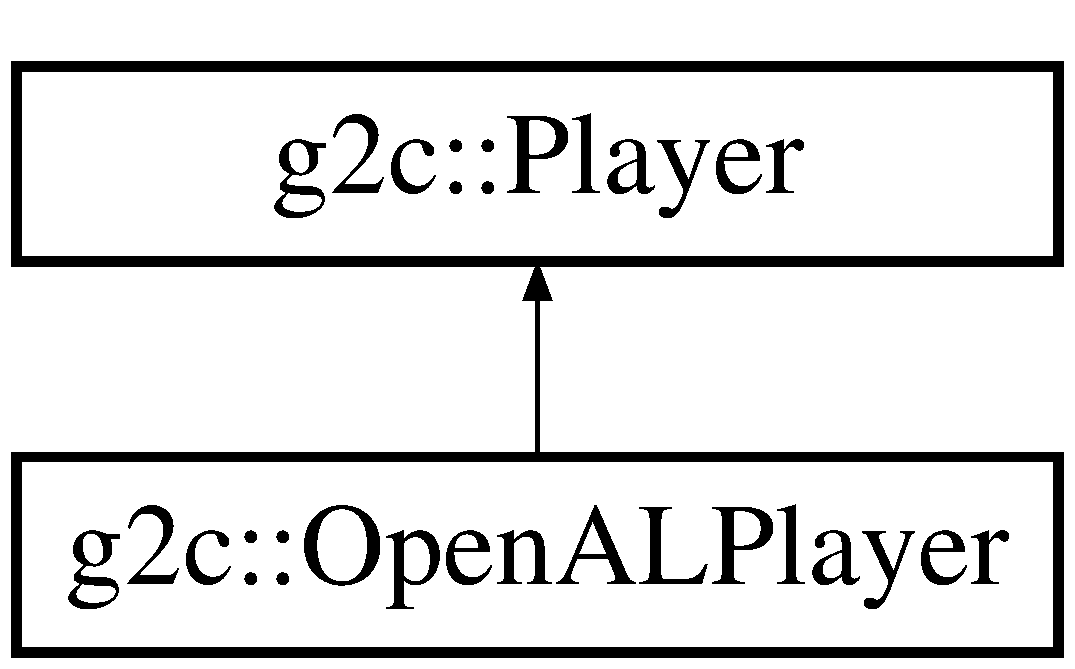
\includegraphics[height=2cm]{classg2c_1_1_open_a_l_player}
\end{center}
\end{figure}
\subsection*{Classes}
\begin{DoxyCompactItemize}
\item 
struct {\bfseries ContextInfo}
\end{DoxyCompactItemize}
\subsection*{Public Member Functions}
\begin{DoxyCompactItemize}
\item 
\hypertarget{classg2c_1_1_open_a_l_player_ade018a5363a49794a61bcd822ff9c12f}{
virtual int {\bfseries createContext} ()}
\label{classg2c_1_1_open_a_l_player_ade018a5363a49794a61bcd822ff9c12f}

\item 
\hypertarget{classg2c_1_1_open_a_l_player_ab898c98689f02f5182a0a3a0fbf193e3}{
virtual void {\bfseries destroyContext} (int index)}
\label{classg2c_1_1_open_a_l_player_ab898c98689f02f5182a0a3a0fbf193e3}

\item 
\hypertarget{classg2c_1_1_open_a_l_player_a9078ebf0bf29d4ac5065c364da711daa}{
virtual int {\bfseries createSource} ()}
\label{classg2c_1_1_open_a_l_player_a9078ebf0bf29d4ac5065c364da711daa}

\item 
\hypertarget{classg2c_1_1_open_a_l_player_af00d372566e0489daf2b1dfe0ec801c1}{
virtual void {\bfseries destroySource} (int index)}
\label{classg2c_1_1_open_a_l_player_af00d372566e0489daf2b1dfe0ec801c1}

\item 
\hypertarget{classg2c_1_1_open_a_l_player_ae2bc1c052312e2177f34192c428dc14e}{
virtual int {\bfseries createSound} ()}
\label{classg2c_1_1_open_a_l_player_ae2bc1c052312e2177f34192c428dc14e}

\item 
\hypertarget{classg2c_1_1_open_a_l_player_a62a2b612987819153ac5fb1b719bbd30}{
virtual void {\bfseries destroySound} (int index)}
\label{classg2c_1_1_open_a_l_player_a62a2b612987819153ac5fb1b719bbd30}

\item 
\hypertarget{classg2c_1_1_open_a_l_player_acdd3ad6b39141fb940c18ef88d626153}{
virtual void {\bfseries makeContextCurrent} (int index)}
\label{classg2c_1_1_open_a_l_player_acdd3ad6b39141fb940c18ef88d626153}

\item 
\hypertarget{classg2c_1_1_open_a_l_player_a80e15f9a0e5980df64d658260f32cd9c}{
virtual bool {\bfseries isSourcePlaying} (int index)}
\label{classg2c_1_1_open_a_l_player_a80e15f9a0e5980df64d658260f32cd9c}

\item 
\hypertarget{classg2c_1_1_open_a_l_player_a97eee57bb99b76ea0a3ae93d69a12d7b}{
virtual void {\bfseries stopSource} (int index)}
\label{classg2c_1_1_open_a_l_player_a97eee57bb99b76ea0a3ae93d69a12d7b}

\item 
\hypertarget{classg2c_1_1_open_a_l_player_aab9a0225972c9dd7a03b27d073ef713b}{
virtual void {\bfseries loadSound} (int index, int sampleRate, int numSamples, int numChannels, int bytesPerSample, uint8\_\-t $\ast$data)}
\label{classg2c_1_1_open_a_l_player_aab9a0225972c9dd7a03b27d073ef713b}

\item 
\hypertarget{classg2c_1_1_open_a_l_player_a3501ac69bb3025b2aeb7b804be65d6c0}{
virtual void {\bfseries playSound} (int soundIndex, int sourceIndex, bool loop, double gain)}
\label{classg2c_1_1_open_a_l_player_a3501ac69bb3025b2aeb7b804be65d6c0}

\end{DoxyCompactItemize}


The documentation for this class was generated from the following files:\begin{DoxyCompactItemize}
\item 
openalplayer.h\item 
openalplayer.cpp\end{DoxyCompactItemize}

\hypertarget{classg2c_1_1_player}{
\section{g2c::Player Class Reference}
\label{classg2c_1_1_player}\index{g2c::Player@{g2c::Player}}
}
Inheritance diagram for g2c::Player::\begin{figure}[H]
\begin{center}
\leavevmode
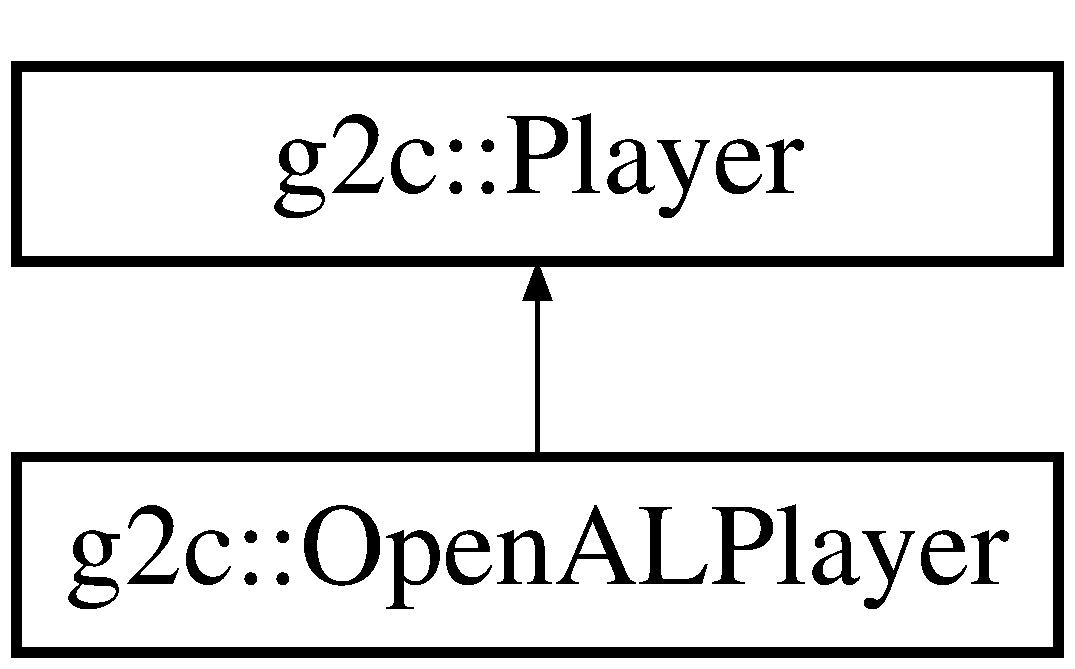
\includegraphics[height=2cm]{classg2c_1_1_player}
\end{center}
\end{figure}
\subsection*{Public Member Functions}
\begin{DoxyCompactItemize}
\item 
\hypertarget{classg2c_1_1_player_aa7a100a15b6cf684707516a644086c23}{
virtual int {\bfseries createContext} ()=0}
\label{classg2c_1_1_player_aa7a100a15b6cf684707516a644086c23}

\item 
\hypertarget{classg2c_1_1_player_abe5399d1e309a9f54776f3a931b08fb3}{
virtual void {\bfseries destroyContext} (int index)=0}
\label{classg2c_1_1_player_abe5399d1e309a9f54776f3a931b08fb3}

\item 
\hypertarget{classg2c_1_1_player_aa36458a27d9b8129ab1b9e01cdcf985b}{
virtual int {\bfseries createSource} ()=0}
\label{classg2c_1_1_player_aa36458a27d9b8129ab1b9e01cdcf985b}

\item 
\hypertarget{classg2c_1_1_player_ab45f2395c2ad343dc5315d4734018fde}{
virtual void {\bfseries destroySource} (int index)=0}
\label{classg2c_1_1_player_ab45f2395c2ad343dc5315d4734018fde}

\item 
\hypertarget{classg2c_1_1_player_a92af47935538ed4a64f35dd926f6625e}{
virtual int {\bfseries createSound} ()=0}
\label{classg2c_1_1_player_a92af47935538ed4a64f35dd926f6625e}

\item 
\hypertarget{classg2c_1_1_player_a6743fdc2e61ea1dd5aff7cec08c59828}{
virtual void {\bfseries destroySound} (int index)=0}
\label{classg2c_1_1_player_a6743fdc2e61ea1dd5aff7cec08c59828}

\item 
\hypertarget{classg2c_1_1_player_ad936c96127a0592741ba1f7afd8e89fa}{
virtual void {\bfseries makeContextCurrent} (int index)=0}
\label{classg2c_1_1_player_ad936c96127a0592741ba1f7afd8e89fa}

\item 
\hypertarget{classg2c_1_1_player_a66492c203fce691cd7a671ee24188f05}{
virtual bool {\bfseries isSourcePlaying} (int index)=0}
\label{classg2c_1_1_player_a66492c203fce691cd7a671ee24188f05}

\item 
\hypertarget{classg2c_1_1_player_a77f9bbc3b34d7c2389fd6dcff3b479ef}{
virtual void {\bfseries stopSource} (int index)=0}
\label{classg2c_1_1_player_a77f9bbc3b34d7c2389fd6dcff3b479ef}

\item 
\hypertarget{classg2c_1_1_player_aabb1086f5b4825b751f9269e0f94bc80}{
virtual void {\bfseries loadSound} (int index, int sampleRate, int numSamples, int numChannels, int bytesPerSample, uint8\_\-t $\ast$data)=0}
\label{classg2c_1_1_player_aabb1086f5b4825b751f9269e0f94bc80}

\item 
\hypertarget{classg2c_1_1_player_a057cc6517be7a061b5bb47452410c9c4}{
virtual void {\bfseries playSound} (int soundIndex, int sourceIndex, bool loop, double gain)=0}
\label{classg2c_1_1_player_a057cc6517be7a061b5bb47452410c9c4}

\end{DoxyCompactItemize}


The documentation for this class was generated from the following files:\begin{DoxyCompactItemize}
\item 
player.h\item 
player.cpp\end{DoxyCompactItemize}

\hypertarget{classg2c_1_1_pointer_vector_property}{
\section{g2c::PointerVectorProperty$<$ T $>$ Class Template Reference}
\label{classg2c_1_1_pointer_vector_property}\index{g2c::PointerVectorProperty@{g2c::PointerVectorProperty}}
}
Inheritance diagram for g2c::PointerVectorProperty$<$ T $>$::\begin{figure}[H]
\begin{center}
\leavevmode
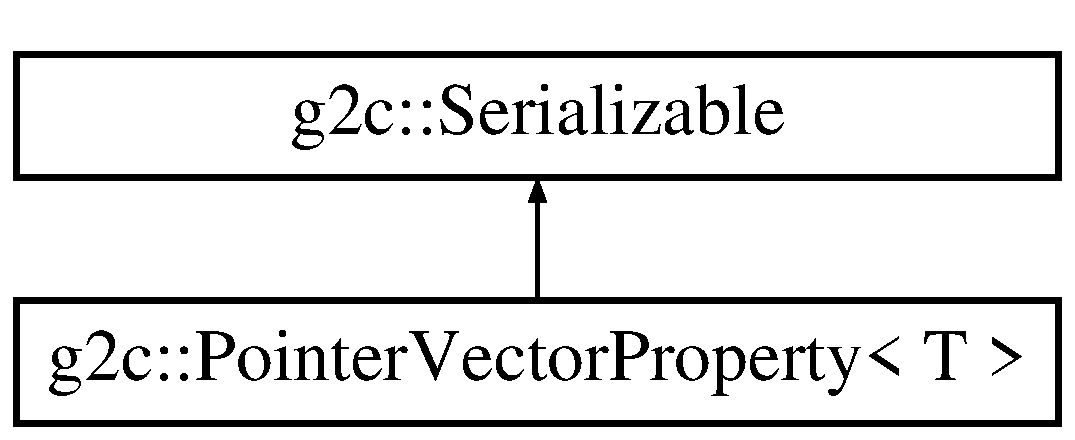
\includegraphics[height=2cm]{classg2c_1_1_pointer_vector_property}
\end{center}
\end{figure}
\subsection*{Public Member Functions}
\begin{DoxyCompactItemize}
\item 
\hypertarget{classg2c_1_1_pointer_vector_property_a491789e14f8e44a03ddda05dccd6ca14}{
{\bfseries PointerVectorProperty} (const std::vector$<$ T $>$ \&v)}
\label{classg2c_1_1_pointer_vector_property_a491789e14f8e44a03ddda05dccd6ca14}

\item 
\hypertarget{classg2c_1_1_pointer_vector_property_aa614e7b7bbf0a78a199fbe551fbcf1d8}{
virtual std::string {\bfseries serialize} (std::string indent=\char`\"{}\char`\"{}) const }
\label{classg2c_1_1_pointer_vector_property_aa614e7b7bbf0a78a199fbe551fbcf1d8}

\item 
\hypertarget{classg2c_1_1_pointer_vector_property_a905e58573f0eefe7f8ad5fd88dca2d81}{
void {\bfseries initWithParseNode} (const \hyperlink{classparse_1_1_node}{parse::Node} $\ast$n)}
\label{classg2c_1_1_pointer_vector_property_a905e58573f0eefe7f8ad5fd88dca2d81}

\end{DoxyCompactItemize}
\subsubsection*{template$<$class T$>$ class g2c::PointerVectorProperty$<$ T $>$}



The documentation for this class was generated from the following file:\begin{DoxyCompactItemize}
\item 
serializable.h\end{DoxyCompactItemize}

\hypertarget{classg2c_1_1_polygon}{
\section{g2c::Polygon Class Reference}
\label{classg2c_1_1_polygon}\index{g2c::Polygon@{g2c::Polygon}}
}
Inheritance diagram for g2c::Polygon::\begin{figure}[H]
\begin{center}
\leavevmode
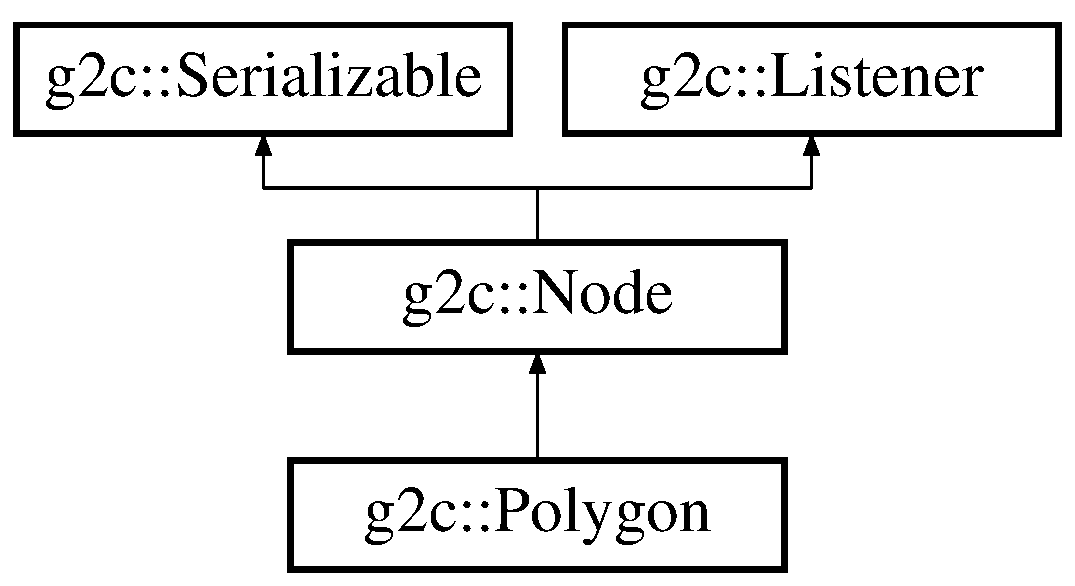
\includegraphics[height=3cm]{classg2c_1_1_polygon}
\end{center}
\end{figure}
\subsection*{Public Types}
\begin{DoxyCompactItemize}
\item 
enum {\bfseries DrawType} \{ {\bfseries kSolid}, 
{\bfseries kOutline}
 \}
\end{DoxyCompactItemize}
\subsection*{Public Member Functions}
\begin{DoxyCompactItemize}
\item 
\hypertarget{classg2c_1_1_polygon_aa44b8ce94bdad2fdf0984c4e8e0b66d3}{
{\bfseries Polygon} (const \hyperlink{classg2c_1_1_polygon}{Polygon} \&P)}
\label{classg2c_1_1_polygon_aa44b8ce94bdad2fdf0984c4e8e0b66d3}

\item 
\hypertarget{classg2c_1_1_polygon_a5f1cb502b4b90fa770ff08efa04c59ff}{
\hyperlink{classg2c_1_1_polygon}{Polygon} \& {\bfseries operator=} (const \hyperlink{classg2c_1_1_polygon}{Polygon} \&P)}
\label{classg2c_1_1_polygon_a5f1cb502b4b90fa770ff08efa04c59ff}

\item 
\hypertarget{classg2c_1_1_polygon_ad565ed0ec7a721969bc1df7326f0a7da}{
\hyperlink{classg2c_1_1_polygon}{Polygon} \& {\bfseries add} (const Vec2 \&V)}
\label{classg2c_1_1_polygon_ad565ed0ec7a721969bc1df7326f0a7da}

\item 
\hypertarget{classg2c_1_1_polygon_a208febc8148a57dd0912c4f6b97d95db}{
\hyperlink{classg2c_1_1_polygon}{Polygon} \& {\bfseries add} (double x, double y)}
\label{classg2c_1_1_polygon_a208febc8148a57dd0912c4f6b97d95db}

\item 
\hypertarget{classg2c_1_1_polygon_a1fb95a077fc91fbe5ae86a377c9edf55}{
\hyperlink{classg2c_1_1_polygon}{Polygon} \& {\bfseries operator+=} (const Vec2 \&V)}
\label{classg2c_1_1_polygon_a1fb95a077fc91fbe5ae86a377c9edf55}

\item 
\hypertarget{classg2c_1_1_polygon_a03d8e3d600d205261f329c2bdab3fc63}{
\hyperlink{classg2c_1_1_polygon}{Polygon} \& {\bfseries operator-\/=} (const Vec2 \&V)}
\label{classg2c_1_1_polygon_a03d8e3d600d205261f329c2bdab3fc63}

\item 
\hypertarget{classg2c_1_1_polygon_afae4fbaf257bac8219b8daee2b3fd8c4}{
\hyperlink{classg2c_1_1_polygon}{Polygon} \& {\bfseries operator$\ast$=} (double k)}
\label{classg2c_1_1_polygon_afae4fbaf257bac8219b8daee2b3fd8c4}

\item 
\hypertarget{classg2c_1_1_polygon_af57063988da8fd591774a5b33702ca8f}{
\hyperlink{classg2c_1_1_polygon}{Polygon} \& {\bfseries operator/=} (double k)}
\label{classg2c_1_1_polygon_af57063988da8fd591774a5b33702ca8f}

\item 
\hypertarget{classg2c_1_1_polygon_a3b95c317b1725ac35d7609e80b40c872}{
\hyperlink{classg2c_1_1_polygon}{Polygon} {\bfseries operator+} (const Vec2 \&V) const }
\label{classg2c_1_1_polygon_a3b95c317b1725ac35d7609e80b40c872}

\item 
\hypertarget{classg2c_1_1_polygon_ad802be08ccb52c26ccce0914c69ade4a}{
\hyperlink{classg2c_1_1_polygon}{Polygon} {\bfseries operator-\/} (const Vec2 \&V) const }
\label{classg2c_1_1_polygon_ad802be08ccb52c26ccce0914c69ade4a}

\item 
\hypertarget{classg2c_1_1_polygon_aadd858a57915882aa74ffde8642f5dcf}{
\hyperlink{classg2c_1_1_polygon}{Polygon} {\bfseries operator$\ast$} (double k) const }
\label{classg2c_1_1_polygon_aadd858a57915882aa74ffde8642f5dcf}

\item 
\hypertarget{classg2c_1_1_polygon_a8abdf6051440b13a45b54e6ed009adc5}{
\hyperlink{classg2c_1_1_polygon}{Polygon} {\bfseries operator/} (double k) const }
\label{classg2c_1_1_polygon_a8abdf6051440b13a45b54e6ed009adc5}

\item 
\hypertarget{classg2c_1_1_polygon_a73304f75939cc48cbee288b413063668}{
void {\bfseries rotate} (double theta)}
\label{classg2c_1_1_polygon_a73304f75939cc48cbee288b413063668}

\item 
\hypertarget{classg2c_1_1_polygon_af0e5941fad20f8b667469f6f071e6cdf}{
virtual void {\bfseries draw} () const }
\label{classg2c_1_1_polygon_af0e5941fad20f8b667469f6f071e6cdf}

\item 
\hypertarget{classg2c_1_1_polygon_abe399dda79a4d649bde0f344f29062c6}{
std::vector$<$ Vec2 $>$::size\_\-type {\bfseries size} () const }
\label{classg2c_1_1_polygon_abe399dda79a4d649bde0f344f29062c6}

\item 
\hypertarget{classg2c_1_1_polygon_a92913e9720d273ec4a63d83d202e9d18}{
bool {\bfseries empty} () const }
\label{classg2c_1_1_polygon_a92913e9720d273ec4a63d83d202e9d18}

\item 
\hypertarget{classg2c_1_1_polygon_a9ce886c8057af266710925b460491ce1}{
bool {\bfseries vectorInside} (const Vec2 \&V) const }
\label{classg2c_1_1_polygon_a9ce886c8057af266710925b460491ce1}

\item 
\hypertarget{classg2c_1_1_polygon_ac60348bbf39cc756ab0d500907c04cee}{
void {\bfseries reverse} ()}
\label{classg2c_1_1_polygon_ac60348bbf39cc756ab0d500907c04cee}

\item 
\hypertarget{classg2c_1_1_polygon_a2d922954ae58da55a56b95befa1a87c2}{
void {\bfseries setVertices} (const std::vector$<$ Vec2 $>$ \&p)}
\label{classg2c_1_1_polygon_a2d922954ae58da55a56b95befa1a87c2}

\item 
\hypertarget{classg2c_1_1_polygon_ae9160bb2b95bbda133d5997d64353ec7}{
std::vector$<$ Vec2 $>$ {\bfseries getVertices} () const }
\label{classg2c_1_1_polygon_ae9160bb2b95bbda133d5997d64353ec7}

\item 
\hypertarget{classg2c_1_1_polygon_ae83e26d35197dc46fec2d024acd45978}{
DrawType {\bfseries getDrawType} () const }
\label{classg2c_1_1_polygon_ae83e26d35197dc46fec2d024acd45978}

\item 
\hypertarget{classg2c_1_1_polygon_adb8ac9391e5be1530bfcf95cfd815496}{
void {\bfseries setDrawType} (DrawType inDrawType)}
\label{classg2c_1_1_polygon_adb8ac9391e5be1530bfcf95cfd815496}

\item 
\hypertarget{classg2c_1_1_polygon_a757e0759a31ee87c6676c89ebb92db8f}{
virtual void {\bfseries handleChild} (const \hyperlink{classparse_1_1_node}{parse::Node} $\ast$n)}
\label{classg2c_1_1_polygon_a757e0759a31ee87c6676c89ebb92db8f}

\item 
\hypertarget{classg2c_1_1_polygon_a3960ba169b09bf89380f1bdda74111e0}{
virtual std::string {\bfseries serializeElements} (std::string indent=\char`\"{}\char`\"{}) const }
\label{classg2c_1_1_polygon_a3960ba169b09bf89380f1bdda74111e0}

\end{DoxyCompactItemize}
\subsection*{Public Attributes}
\begin{DoxyCompactItemize}
\item 
\hypertarget{classg2c_1_1_polygon_a43201567ddff9189372dbf55f33ec454}{
\hyperlink{classg2c_1_1_vector_property}{VectorProperty}$<$ \hyperlink{classg2c_1_1_vec2_property}{Vec2Property} $>$ {\bfseries vertices}}
\label{classg2c_1_1_polygon_a43201567ddff9189372dbf55f33ec454}

\end{DoxyCompactItemize}
\subsection*{Friends}
\begin{DoxyCompactItemize}
\item 
\hypertarget{classg2c_1_1_polygon_a1c64eb1893a94ae78e7cc470f8531f3f}{
class \hyperlink{classg2c_1_1_polygon}{Polygon} {\bfseries operator$\ast$} (const Mat4 \&, const \hyperlink{classg2c_1_1_polygon}{Polygon} \&P)}
\label{classg2c_1_1_polygon_a1c64eb1893a94ae78e7cc470f8531f3f}

\item 
\hypertarget{classg2c_1_1_polygon_aee40ba04c874821ab064551b0c729561}{
class \hyperlink{classg2c_1_1_polygon}{Polygon} {\bfseries operator$\ast$} (double k, const \hyperlink{classg2c_1_1_polygon}{Polygon} \&P)}
\label{classg2c_1_1_polygon_aee40ba04c874821ab064551b0c729561}

\item 
\hypertarget{classg2c_1_1_polygon_a6c70c2be591e72940dc345f9b357cca6}{
class \hyperlink{classg2c_1_1_polygon}{Polygon} {\bfseries operator+} (const Vec2 \&V, const \hyperlink{classg2c_1_1_polygon}{Polygon} \&P)}
\label{classg2c_1_1_polygon_a6c70c2be591e72940dc345f9b357cca6}

\end{DoxyCompactItemize}


The documentation for this class was generated from the following files:\begin{DoxyCompactItemize}
\item 
sprites.h\item 
sprites.cpp\end{DoxyCompactItemize}

\hypertarget{classg2c_1_1_renderer}{
\section{g2c::Renderer Class Reference}
\label{classg2c_1_1_renderer}\index{g2c::Renderer@{g2c::Renderer}}
}


{\ttfamily \#include $<$sprites.h$>$}Inheritance diagram for g2c::Renderer::\begin{figure}[H]
\begin{center}
\leavevmode
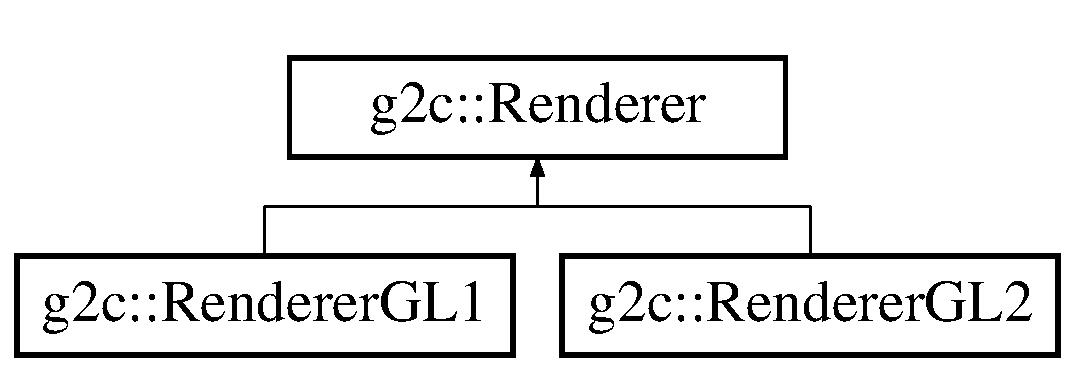
\includegraphics[height=2cm]{classg2c_1_1_renderer}
\end{center}
\end{figure}
\subsection*{Public Member Functions}
\begin{DoxyCompactItemize}
\item 
virtual void \hyperlink{classg2c_1_1_renderer_adcfacb02cf062a77f0fb71ab30dbae76}{init} ()=0
\item 
virtual void \hyperlink{classg2c_1_1_renderer_a60445bc0c7ec75f1c7ee20066c25f8b3}{drawMesh} (const \hyperlink{classg2c_1_1_mesh}{Mesh} $\ast$mesh, const Mat4 \&matrix, const Mat3 \&texMatrix, const \hyperlink{classg2c_1_1_color}{Color} \&color, const \hyperlink{classg2c_1_1_texture}{Texture} $\ast$texture) const =0
\item 
\hypertarget{classg2c_1_1_renderer_abad3c83e4ff3b8f5ee28f1a26d773e1d}{
virtual void {\bfseries drawMesh} (const \hyperlink{classg2c_1_1_mesh}{Mesh} $\ast$m, const \hyperlink{classg2c_1_1_node}{Node} $\ast$n) const }
\label{classg2c_1_1_renderer_abad3c83e4ff3b8f5ee28f1a26d773e1d}

\end{DoxyCompactItemize}
\subsection*{Public Attributes}
\begin{DoxyCompactItemize}
\item 
\hypertarget{classg2c_1_1_renderer_aa0b929f6031e291d17c53c4565f40525}{
Mat4 {\bfseries projection}}
\label{classg2c_1_1_renderer_aa0b929f6031e291d17c53c4565f40525}

\end{DoxyCompactItemize}
\subsection*{Protected Attributes}
\begin{DoxyCompactItemize}
\item 
\hypertarget{classg2c_1_1_renderer_a4c3de633fedb9d5e738562a6bf126263}{
GLfloat {\bfseries fv} \mbox{[}16\mbox{]}}
\label{classg2c_1_1_renderer_a4c3de633fedb9d5e738562a6bf126263}

\item 
\hypertarget{classg2c_1_1_renderer_aec68eba790008ede3415b734d891075e}{
\hyperlink{classg2c_1_1_mesh}{Mesh} $\ast$ {\bfseries quad}}
\label{classg2c_1_1_renderer_aec68eba790008ede3415b734d891075e}

\end{DoxyCompactItemize}


\subsection{Detailed Description}
\hyperlink{classg2c_1_1_renderer}{Renderer} is an abstract base-\/class whose virtual methods define how a \hyperlink{classg2c_1_1_mesh}{Mesh} shall be drawn. Subclasses of \hyperlink{classg2c_1_1_renderer}{Renderer} represent a scheme for drawing a mesh in a particular graphics library.

To implement a renderer, implement \hyperlink{classg2c_1_1_renderer_adcfacb02cf062a77f0fb71ab30dbae76}{init()} and \hyperlink{classg2c_1_1_renderer_a60445bc0c7ec75f1c7ee20066c25f8b3}{drawMesh()}. Whichever renderer Sprite::renderer is set to gets used to draw all sprite graphics. 

\subsection{Member Function Documentation}
\hypertarget{classg2c_1_1_renderer_a60445bc0c7ec75f1c7ee20066c25f8b3}{
\index{g2c::Renderer@{g2c::Renderer}!drawMesh@{drawMesh}}
\index{drawMesh@{drawMesh}!g2c::Renderer@{g2c::Renderer}}
\subsubsection[{drawMesh}]{\setlength{\rightskip}{0pt plus 5cm}virtual void g2c::Renderer::drawMesh (const {\bf Mesh} $\ast$ {\em mesh}, \/  const Mat4 \& {\em matrix}, \/  const Mat3 \& {\em texMatrix}, \/  const {\bf Color} \& {\em color}, \/  const {\bf Texture} $\ast$ {\em texture}) const\hspace{0.3cm}{\ttfamily  \mbox{[}pure virtual\mbox{]}}}}
\label{classg2c_1_1_renderer_a60445bc0c7ec75f1c7ee20066c25f8b3}
Overridden to draw a \hyperlink{classg2c_1_1_mesh}{Mesh} object. If mesh is NULL, drawMesh must still draw a default unit square. 

Implemented in \hyperlink{classg2c_1_1_renderer_g_l1_a26b67e30372294a022b981fa6b0d76c4}{g2c::RendererGL1}, and \hyperlink{classg2c_1_1_renderer_g_l2_a42c4be1e991664f9a2ba8ef013cb00c1}{g2c::RendererGL2}.\hypertarget{classg2c_1_1_renderer_adcfacb02cf062a77f0fb71ab30dbae76}{
\index{g2c::Renderer@{g2c::Renderer}!init@{init}}
\index{init@{init}!g2c::Renderer@{g2c::Renderer}}
\subsubsection[{init}]{\setlength{\rightskip}{0pt plus 5cm}virtual void g2c::Renderer::init ()\hspace{0.3cm}{\ttfamily  \mbox{[}pure virtual\mbox{]}}}}
\label{classg2c_1_1_renderer_adcfacb02cf062a77f0fb71ab30dbae76}
Overridden to initialize the renderer. 

Implemented in \hyperlink{classg2c_1_1_renderer_g_l1_a3577eea69cf61c38dc3595b24251fab7}{g2c::RendererGL1}, and \hyperlink{classg2c_1_1_renderer_g_l2_acd65c8c77dbecbe19c2bb19ef3847ce5}{g2c::RendererGL2}.

The documentation for this class was generated from the following files:\begin{DoxyCompactItemize}
\item 
sprites.h\item 
sprites.cpp\end{DoxyCompactItemize}

\hypertarget{classg2c_1_1_renderer_g_l1}{
\section{g2c::RendererGL1 Class Reference}
\label{classg2c_1_1_renderer_g_l1}\index{g2c::RendererGL1@{g2c::RendererGL1}}
}


{\ttfamily \#include $<$sprites.h$>$}Inheritance diagram for g2c::RendererGL1::\begin{figure}[H]
\begin{center}
\leavevmode
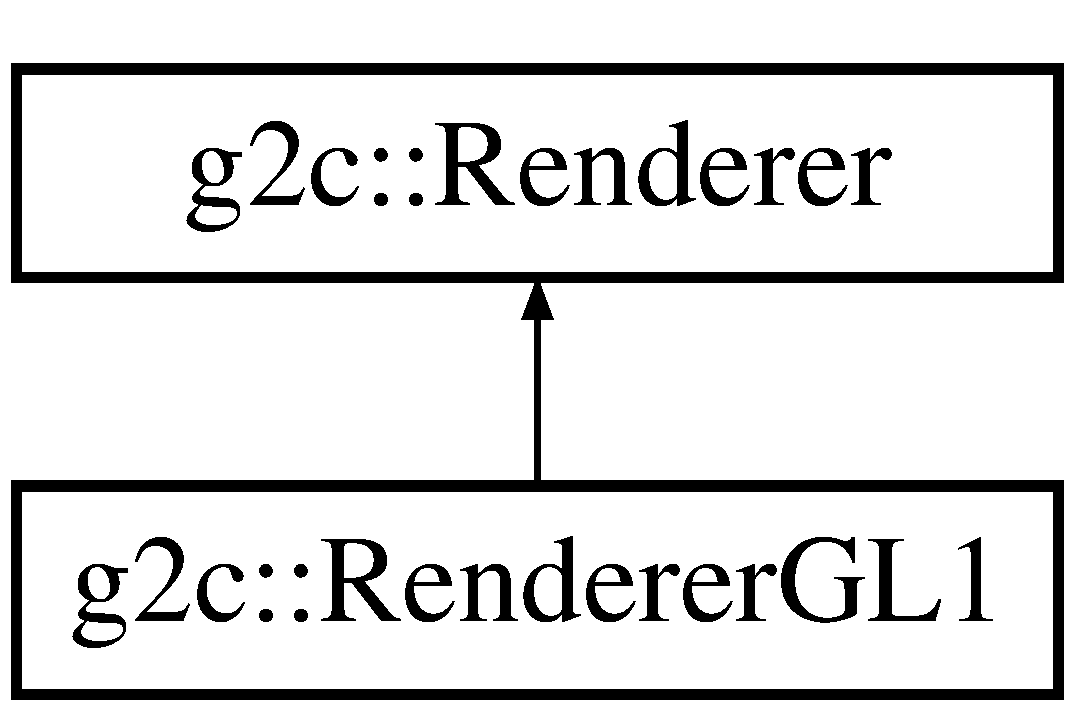
\includegraphics[height=2cm]{classg2c_1_1_renderer_g_l1}
\end{center}
\end{figure}
\subsection*{Public Member Functions}
\begin{DoxyCompactItemize}
\item 
virtual void \hyperlink{classg2c_1_1_renderer_g_l1_a3577eea69cf61c38dc3595b24251fab7}{init} ()
\item 
virtual void \hyperlink{classg2c_1_1_renderer_g_l1_a26b67e30372294a022b981fa6b0d76c4}{drawMesh} (const \hyperlink{classg2c_1_1_mesh}{Mesh} $\ast$mesh, const Mat4 \&matrix, const Mat3 \&texMatrix, const \hyperlink{classg2c_1_1_color}{Color} \&color, const \hyperlink{classg2c_1_1_texture}{Texture} $\ast$texture) const 
\end{DoxyCompactItemize}


\subsection{Detailed Description}
An implementation of \hyperlink{classg2c_1_1_renderer}{Renderer} to draw meshes using OpenGL calls from the OpenGL ES 1 collection. The draw function in this will work in desktop OpenGL or in OpenGL ES 1.

Set Sprite::renderer to an instance of \hyperlink{classg2c_1_1_renderer_g_l1}{RendererGL1} to and call \hyperlink{classg2c_1_1_renderer_g_l1_a3577eea69cf61c38dc3595b24251fab7}{init()}. Then all meshes will draw using it. 

\subsection{Member Function Documentation}
\hypertarget{classg2c_1_1_renderer_g_l1_a26b67e30372294a022b981fa6b0d76c4}{
\index{g2c::RendererGL1@{g2c::RendererGL1}!drawMesh@{drawMesh}}
\index{drawMesh@{drawMesh}!g2c::RendererGL1@{g2c::RendererGL1}}
\subsubsection[{drawMesh}]{\setlength{\rightskip}{0pt plus 5cm}void g2c::RendererGL1::drawMesh (const {\bf Mesh} $\ast$ {\em mesh}, \/  const Mat4 \& {\em matrix}, \/  const Mat3 \& {\em texMatrix}, \/  const {\bf Color} \& {\em color}, \/  const {\bf Texture} $\ast$ {\em texture}) const\hspace{0.3cm}{\ttfamily  \mbox{[}virtual\mbox{]}}}}
\label{classg2c_1_1_renderer_g_l1_a26b67e30372294a022b981fa6b0d76c4}
Overridden to draw a \hyperlink{classg2c_1_1_mesh}{Mesh} object. If mesh is NULL, drawMesh must still draw a default unit square. 

Implements \hyperlink{classg2c_1_1_renderer_a60445bc0c7ec75f1c7ee20066c25f8b3}{g2c::Renderer}.\hypertarget{classg2c_1_1_renderer_g_l1_a3577eea69cf61c38dc3595b24251fab7}{
\index{g2c::RendererGL1@{g2c::RendererGL1}!init@{init}}
\index{init@{init}!g2c::RendererGL1@{g2c::RendererGL1}}
\subsubsection[{init}]{\setlength{\rightskip}{0pt plus 5cm}void g2c::RendererGL1::init ()\hspace{0.3cm}{\ttfamily  \mbox{[}virtual\mbox{]}}}}
\label{classg2c_1_1_renderer_g_l1_a3577eea69cf61c38dc3595b24251fab7}
Overridden to initialize the renderer. 

Implements \hyperlink{classg2c_1_1_renderer_adcfacb02cf062a77f0fb71ab30dbae76}{g2c::Renderer}.

The documentation for this class was generated from the following files:\begin{DoxyCompactItemize}
\item 
sprites.h\item 
sprites.cpp\end{DoxyCompactItemize}

\hypertarget{classg2c_1_1_renderer_g_l2}{
\section{g2c::RendererGL2 Class Reference}
\label{classg2c_1_1_renderer_g_l2}\index{g2c::RendererGL2@{g2c::RendererGL2}}
}


{\ttfamily \#include $<$sprites.h$>$}Inheritance diagram for g2c::RendererGL2::\begin{figure}[H]
\begin{center}
\leavevmode
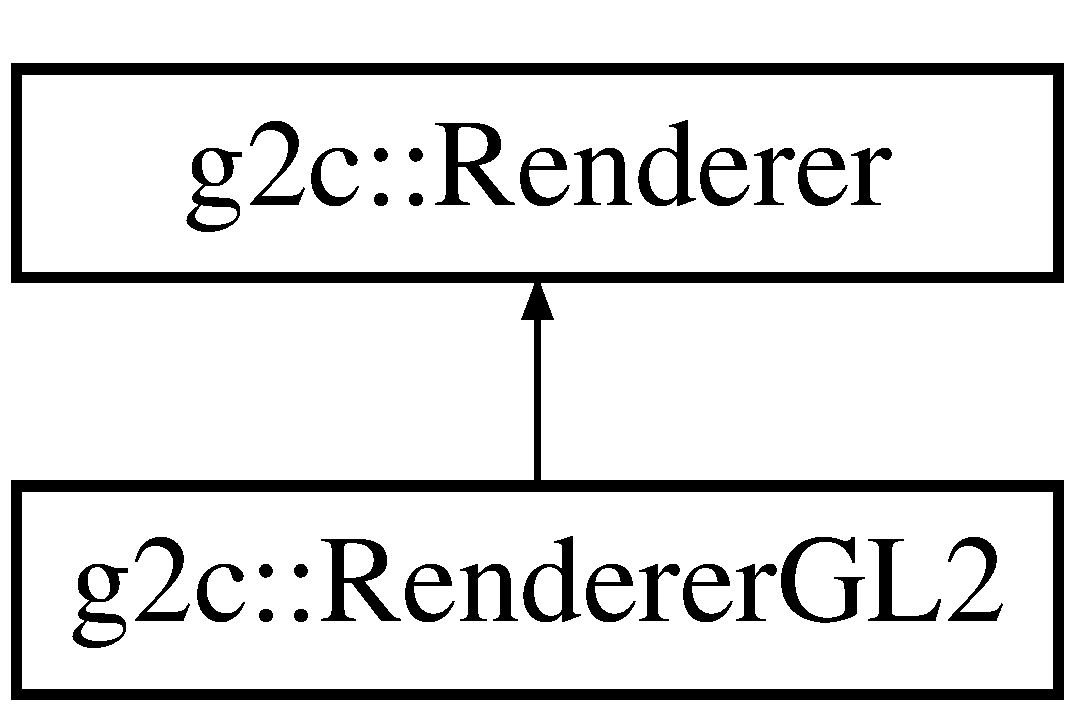
\includegraphics[height=2cm]{classg2c_1_1_renderer_g_l2}
\end{center}
\end{figure}
\subsection*{Public Member Functions}
\begin{DoxyCompactItemize}
\item 
virtual void \hyperlink{classg2c_1_1_renderer_g_l2_acd65c8c77dbecbe19c2bb19ef3847ce5}{init} ()
\end{DoxyCompactItemize}
\subsection*{Protected Member Functions}
\begin{DoxyCompactItemize}
\item 
virtual void \hyperlink{classg2c_1_1_renderer_g_l2_a42c4be1e991664f9a2ba8ef013cb00c1}{drawMesh} (const \hyperlink{classg2c_1_1_mesh}{Mesh} $\ast$m, const Mat4 \&matrix, const Mat3 \&texMatrix, const \hyperlink{classg2c_1_1_color}{Color} \&color, const \hyperlink{classg2c_1_1_texture}{Texture} $\ast$texture) const 
\end{DoxyCompactItemize}
\subsection*{Protected Attributes}
\begin{DoxyCompactItemize}
\item 
\hypertarget{classg2c_1_1_renderer_g_l2_a437787e58e897d930dcebed42f1be546}{
bool {\bfseries initialized}}
\label{classg2c_1_1_renderer_g_l2_a437787e58e897d930dcebed42f1be546}

\end{DoxyCompactItemize}


\subsection{Detailed Description}
An implementation of \hyperlink{classg2c_1_1_renderer}{Renderer} to draw meshes using OpenGL calls from the OpenGL ES 2 collection. The draw function in this will work in desktop OpenGL or in OpenGL ES 2.

Set Sprite::renderer to an instance of \hyperlink{classg2c_1_1_renderer_g_l2}{RendererGL2} to and call \hyperlink{classg2c_1_1_renderer_g_l2_acd65c8c77dbecbe19c2bb19ef3847ce5}{init()}. Then all meshes will draw using it. 

\subsection{Member Function Documentation}
\hypertarget{classg2c_1_1_renderer_g_l2_a42c4be1e991664f9a2ba8ef013cb00c1}{
\index{g2c::RendererGL2@{g2c::RendererGL2}!drawMesh@{drawMesh}}
\index{drawMesh@{drawMesh}!g2c::RendererGL2@{g2c::RendererGL2}}
\subsubsection[{drawMesh}]{\setlength{\rightskip}{0pt plus 5cm}void g2c::RendererGL2::drawMesh (const {\bf Mesh} $\ast$ {\em mesh}, \/  const Mat4 \& {\em matrix}, \/  const Mat3 \& {\em texMatrix}, \/  const {\bf Color} \& {\em color}, \/  const {\bf Texture} $\ast$ {\em texture}) const\hspace{0.3cm}{\ttfamily  \mbox{[}protected, virtual\mbox{]}}}}
\label{classg2c_1_1_renderer_g_l2_a42c4be1e991664f9a2ba8ef013cb00c1}
Overridden to draw a \hyperlink{classg2c_1_1_mesh}{Mesh} object. If mesh is NULL, drawMesh must still draw a default unit square. 

Implements \hyperlink{classg2c_1_1_renderer_a60445bc0c7ec75f1c7ee20066c25f8b3}{g2c::Renderer}.\hypertarget{classg2c_1_1_renderer_g_l2_acd65c8c77dbecbe19c2bb19ef3847ce5}{
\index{g2c::RendererGL2@{g2c::RendererGL2}!init@{init}}
\index{init@{init}!g2c::RendererGL2@{g2c::RendererGL2}}
\subsubsection[{init}]{\setlength{\rightskip}{0pt plus 5cm}void g2c::RendererGL2::init ()\hspace{0.3cm}{\ttfamily  \mbox{[}virtual\mbox{]}}}}
\label{classg2c_1_1_renderer_g_l2_acd65c8c77dbecbe19c2bb19ef3847ce5}
Overridden to initialize the renderer. 

Implements \hyperlink{classg2c_1_1_renderer_adcfacb02cf062a77f0fb71ab30dbae76}{g2c::Renderer}.

The documentation for this class was generated from the following files:\begin{DoxyCompactItemize}
\item 
sprites.h\item 
sprites.cpp\end{DoxyCompactItemize}

\hypertarget{struct_riff_header}{
\section{RiffHeader Struct Reference}
\label{struct_riff_header}\index{RiffHeader@{RiffHeader}}
}
\subsection*{Public Attributes}
\begin{DoxyCompactItemize}
\item 
\hypertarget{struct_riff_header_a5d225f7d82b9b4b2347ce516492b2461}{
char {\bfseries riffTag} \mbox{[}4\mbox{]}}
\label{struct_riff_header_a5d225f7d82b9b4b2347ce516492b2461}

\item 
\hypertarget{struct_riff_header_af9d09b7cc6367dd1042ccdfeffa68aee}{
int {\bfseries chunkSize}}
\label{struct_riff_header_af9d09b7cc6367dd1042ccdfeffa68aee}

\end{DoxyCompactItemize}


The documentation for this struct was generated from the following file:\begin{DoxyCompactItemize}
\item 
wave.cpp\end{DoxyCompactItemize}

\hypertarget{classg2c_1_1_serializable}{
\section{g2c::Serializable Class Reference}
\label{classg2c_1_1_serializable}\index{g2c::Serializable@{g2c::Serializable}}
}
Inheritance diagram for g2c::Serializable::\begin{figure}[H]
\begin{center}
\leavevmode
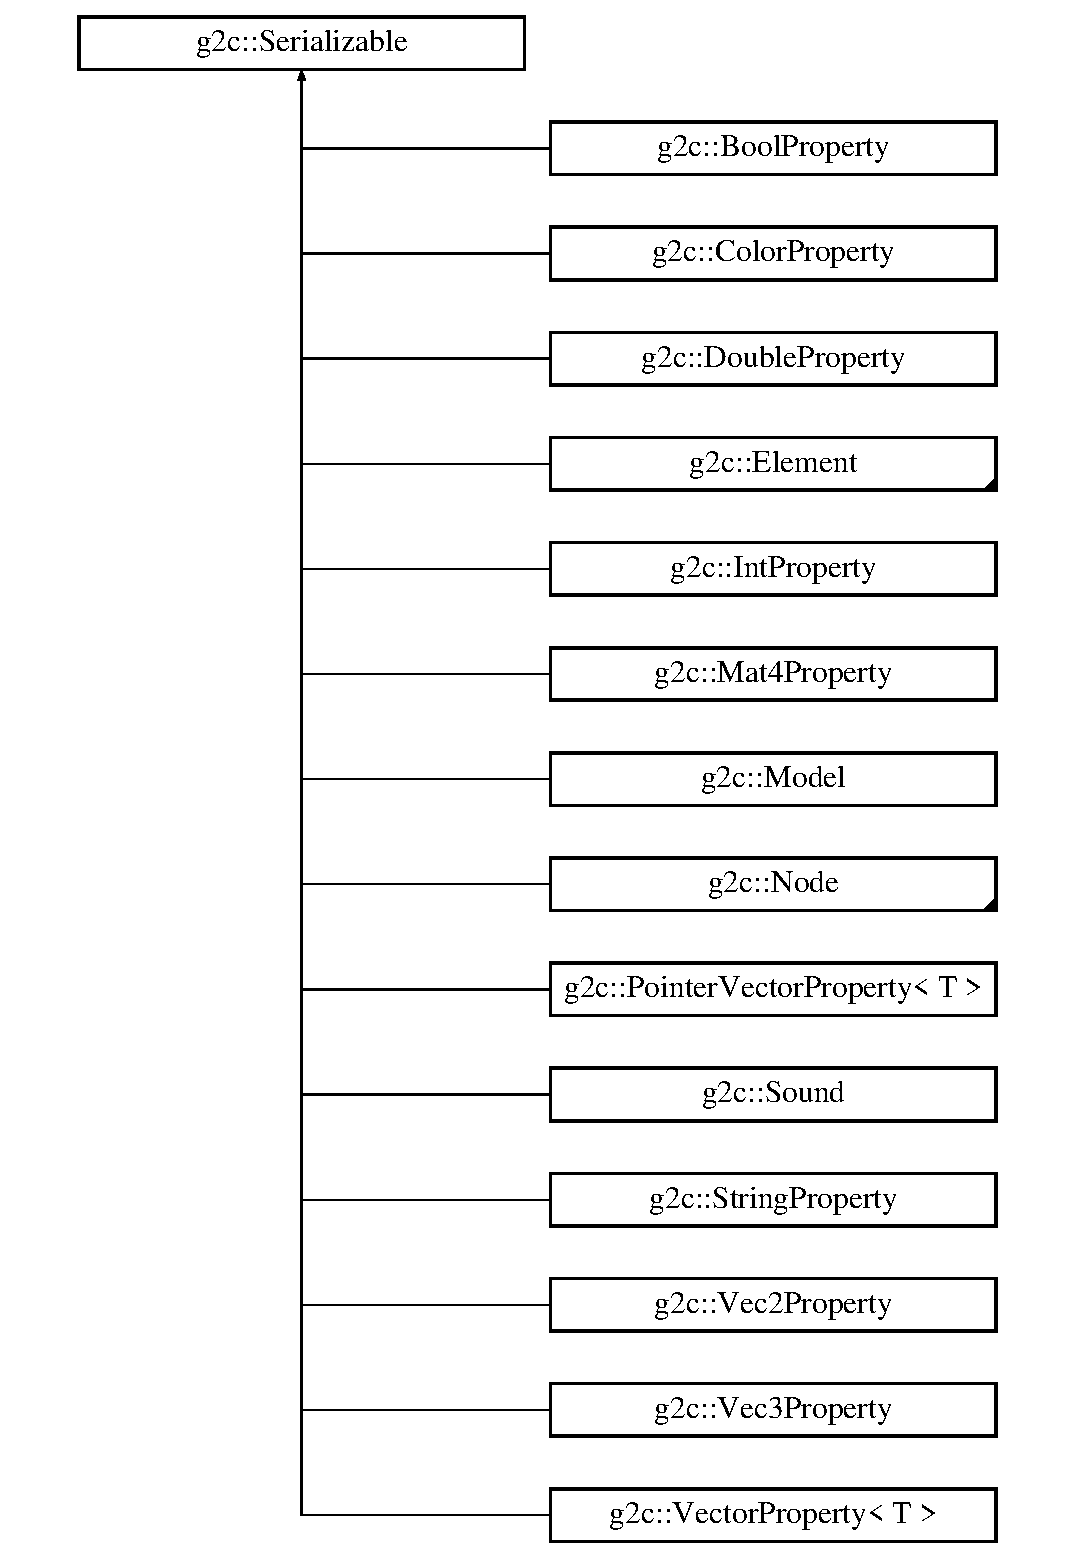
\includegraphics[height=12cm]{classg2c_1_1_serializable}
\end{center}
\end{figure}
\subsection*{Classes}
\begin{DoxyCompactItemize}
\item 
class {\bfseries Property}
\end{DoxyCompactItemize}
\subsection*{Public Member Functions}
\begin{DoxyCompactItemize}
\item 
\hypertarget{classg2c_1_1_serializable_a7703791c3f0b805c89cbf0f2ac745ea8}{
virtual std::string {\bfseries serialize} (std::string indent=\char`\"{}\char`\"{}) const }
\label{classg2c_1_1_serializable_a7703791c3f0b805c89cbf0f2ac745ea8}

\item 
\hypertarget{classg2c_1_1_serializable_a9025ace55eef46cbdb91d9ab89a5af4a}{
virtual void {\bfseries deserialize} (const std::string \&s)}
\label{classg2c_1_1_serializable_a9025ace55eef46cbdb91d9ab89a5af4a}

\item 
\hypertarget{classg2c_1_1_serializable_a8e0e60a1fccff6e2bafac5d40d7d45e2}{
virtual void {\bfseries initWithParseNode} (const \hyperlink{classparse_1_1_node}{parse::Node} $\ast$n)}
\label{classg2c_1_1_serializable_a8e0e60a1fccff6e2bafac5d40d7d45e2}

\item 
\hypertarget{classg2c_1_1_serializable_a2d30ad4c317e19cc6a7185a01f6fbb88}{
std::string {\bfseries getType} (const \hyperlink{classparse_1_1_node}{parse::Node} $\ast$n) const }
\label{classg2c_1_1_serializable_a2d30ad4c317e19cc6a7185a01f6fbb88}

\item 
\hypertarget{classg2c_1_1_serializable_a69085ab8cd1a5954abc9c0d1c0e6924c}{
virtual void {\bfseries handleChild} (const \hyperlink{classparse_1_1_node}{parse::Node} $\ast$n)}
\label{classg2c_1_1_serializable_a69085ab8cd1a5954abc9c0d1c0e6924c}

\item 
\hypertarget{classg2c_1_1_serializable_a5e0751d7aaee57369f22a1908dd3d06c}{
virtual void {\bfseries display} () const }
\label{classg2c_1_1_serializable_a5e0751d7aaee57369f22a1908dd3d06c}

\end{DoxyCompactItemize}
\subsection*{Public Attributes}
\begin{DoxyCompactItemize}
\item 
\hypertarget{classg2c_1_1_serializable_ad853f65bf6ac4d5da473e6697bc864f0}{
std::string {\bfseries type}}
\label{classg2c_1_1_serializable_ad853f65bf6ac4d5da473e6697bc864f0}

\item 
\hypertarget{classg2c_1_1_serializable_a7a677c2891a338e516ba522e63414983}{
std::string {\bfseries name}}
\label{classg2c_1_1_serializable_a7a677c2891a338e516ba522e63414983}

\end{DoxyCompactItemize}
\subsection*{Protected Member Functions}
\begin{DoxyCompactItemize}
\item 
\hypertarget{classg2c_1_1_serializable_af236d2bc1a3dadeee2f5723b4d20ee56}{
virtual std::string {\bfseries serializeBegin} (std::string indent=\char`\"{}\char`\"{}) const }
\label{classg2c_1_1_serializable_af236d2bc1a3dadeee2f5723b4d20ee56}

\item 
\hypertarget{classg2c_1_1_serializable_a53404296d3efe29a8b8b2e6f09e6fbf2}{
virtual std::string {\bfseries serializeElements} (std::string indent=\char`\"{}\char`\"{}) const }
\label{classg2c_1_1_serializable_a53404296d3efe29a8b8b2e6f09e6fbf2}

\item 
\hypertarget{classg2c_1_1_serializable_a20356e175519cdc58b2b81b4135c3385}{
virtual std::string {\bfseries serializeEnd} (std::string indent=\char`\"{}\char`\"{}) const }
\label{classg2c_1_1_serializable_a20356e175519cdc58b2b81b4135c3385}

\item 
\hypertarget{classg2c_1_1_serializable_a1ebd03176b676b7405a37134de7ccfef}{
void {\bfseries addProperty} (const std::string \&name, \hyperlink{classg2c_1_1_serializable}{Serializable} \&element)}
\label{classg2c_1_1_serializable_a1ebd03176b676b7405a37134de7ccfef}

\item 
\hypertarget{classg2c_1_1_serializable_abf5406405e2f51bbff5ac1805e545190}{
void {\bfseries addMember} (const std::string \&name, std::string \&element)}
\label{classg2c_1_1_serializable_abf5406405e2f51bbff5ac1805e545190}

\item 
\hypertarget{classg2c_1_1_serializable_a8af126034d19c9d74f78be17e6bf13f1}{
void {\bfseries addMember} (const std::string \&name, double \&element)}
\label{classg2c_1_1_serializable_a8af126034d19c9d74f78be17e6bf13f1}

\item 
\hypertarget{classg2c_1_1_serializable_a3a0b8ba26cd07e91222335e77aefe15f}{
void {\bfseries addMember} (const std::string \&name, int \&element)}
\label{classg2c_1_1_serializable_a3a0b8ba26cd07e91222335e77aefe15f}

\item 
\hypertarget{classg2c_1_1_serializable_a2a1c97b1f4b6d939f4d7b044d47922f4}{
void {\bfseries addMember} (const std::string \&name, std::vector$<$ double $>$ \&element)}
\label{classg2c_1_1_serializable_a2a1c97b1f4b6d939f4d7b044d47922f4}

\item 
\hypertarget{classg2c_1_1_serializable_aaa28d1e2882c59abedd789d67abefcd9}{
void {\bfseries addMember} (const std::string \&name, std::vector$<$ int $>$ \&element)}
\label{classg2c_1_1_serializable_aaa28d1e2882c59abedd789d67abefcd9}

\item 
\hypertarget{classg2c_1_1_serializable_a9f2781b4b22aa7904bc8447b1adaf544}{
void {\bfseries addMember} (const std::string \&name, std::vector$<$ std::string $>$ \&element)}
\label{classg2c_1_1_serializable_a9f2781b4b22aa7904bc8447b1adaf544}

\end{DoxyCompactItemize}


The documentation for this class was generated from the following files:\begin{DoxyCompactItemize}
\item 
serializable.h\item 
serializable.cpp\end{DoxyCompactItemize}

\hypertarget{classg2c_1_1_shape}{
\section{g2c::Shape Class Reference}
\label{classg2c_1_1_shape}\index{g2c::Shape@{g2c::Shape}}
}
Inheritance diagram for g2c::Shape::\begin{figure}[H]
\begin{center}
\leavevmode
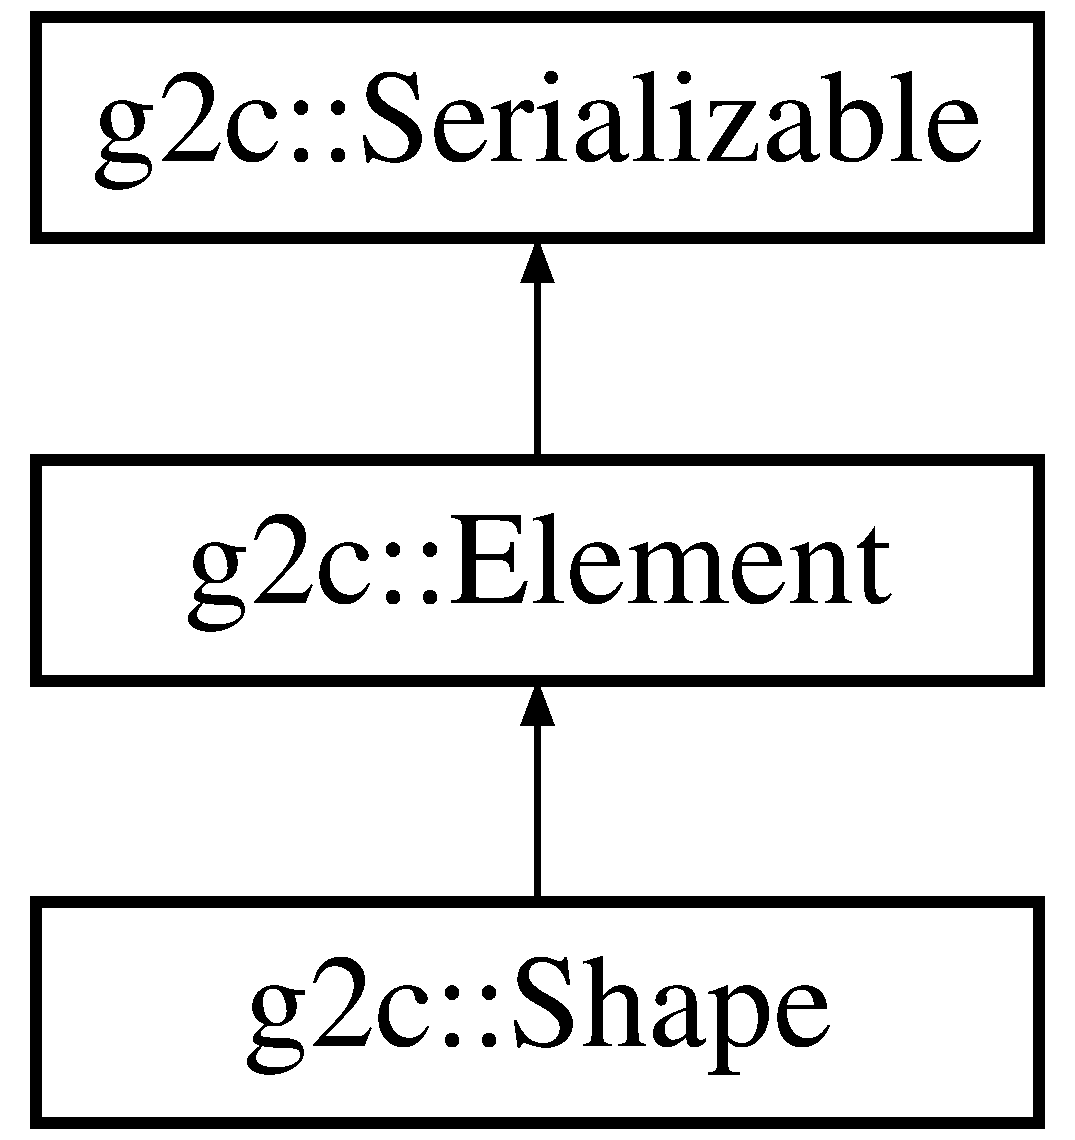
\includegraphics[height=3cm]{classg2c_1_1_shape}
\end{center}
\end{figure}
\subsection*{Public Member Functions}
\begin{DoxyCompactItemize}
\item 
\hypertarget{classg2c_1_1_shape_aac6a51ff8e83b3505176e9b8e19ee20d}{
void {\bfseries draw} () const }
\label{classg2c_1_1_shape_aac6a51ff8e83b3505176e9b8e19ee20d}

\item 
\hypertarget{classg2c_1_1_shape_aeb770b57393650d529f8530fbfe2b881}{
const \hyperlink{classg2c_1_1_value}{Value} \& {\bfseries get} (const std::string \&uniformName) const }
\label{classg2c_1_1_shape_aeb770b57393650d529f8530fbfe2b881}

\end{DoxyCompactItemize}
\subsection*{Public Attributes}
\begin{DoxyCompactItemize}
\item 
\hypertarget{classg2c_1_1_shape_a40588517f441849299c43a80acdfc6d9}{
bool {\bfseries visible}}
\label{classg2c_1_1_shape_a40588517f441849299c43a80acdfc6d9}

\item 
\hypertarget{classg2c_1_1_shape_a549580f86201cd558663ccdb2d0fd4af}{
std::string {\bfseries geometryName}}
\label{classg2c_1_1_shape_a549580f86201cd558663ccdb2d0fd4af}

\item 
\hypertarget{classg2c_1_1_shape_a583dc942f6b2f2c4b6fe4c19c8f6c57c}{
std::vector$<$ std::string $>$ {\bfseries assumptionNames}}
\label{classg2c_1_1_shape_a583dc942f6b2f2c4b6fe4c19c8f6c57c}

\item 
\hypertarget{classg2c_1_1_shape_a7c8a6a3d2a053d73dd9a624f184e12bb}{
\hyperlink{classg2c_1_1_geometry}{Geometry} $\ast$ {\bfseries geometry}}
\label{classg2c_1_1_shape_a7c8a6a3d2a053d73dd9a624f184e12bb}

\item 
\hypertarget{classg2c_1_1_shape_ac589104b26ea0777b5c183d3cf341608}{
std::list$<$ \hyperlink{classg2c_1_1_assumption}{Assumption} $\ast$ $>$ {\bfseries assumptions}}
\label{classg2c_1_1_shape_ac589104b26ea0777b5c183d3cf341608}

\end{DoxyCompactItemize}
\subsection*{Protected Member Functions}
\begin{DoxyCompactItemize}
\item 
\hypertarget{classg2c_1_1_shape_a71a749a93c583fea4bb26f48a0e2fe9e}{
virtual std::string {\bfseries serializeElements} (std::string indent=\char`\"{}\char`\"{}) const }
\label{classg2c_1_1_shape_a71a749a93c583fea4bb26f48a0e2fe9e}

\item 
\hypertarget{classg2c_1_1_shape_ab1070e4d677cb4a0098b11cfe6754cfd}{
virtual void {\bfseries handleChild} (const \hyperlink{classparse_1_1_node}{parse::Node} $\ast$n)}
\label{classg2c_1_1_shape_ab1070e4d677cb4a0098b11cfe6754cfd}

\end{DoxyCompactItemize}


The documentation for this class was generated from the following files:\begin{DoxyCompactItemize}
\item 
graphics.h\item 
graphics.cpp\end{DoxyCompactItemize}

\hypertarget{classg2c_1_1_sound}{
\section{g2c::Sound Class Reference}
\label{classg2c_1_1_sound}\index{g2c::Sound@{g2c::Sound}}
}
Inheritance diagram for g2c::Sound::\begin{figure}[H]
\begin{center}
\leavevmode
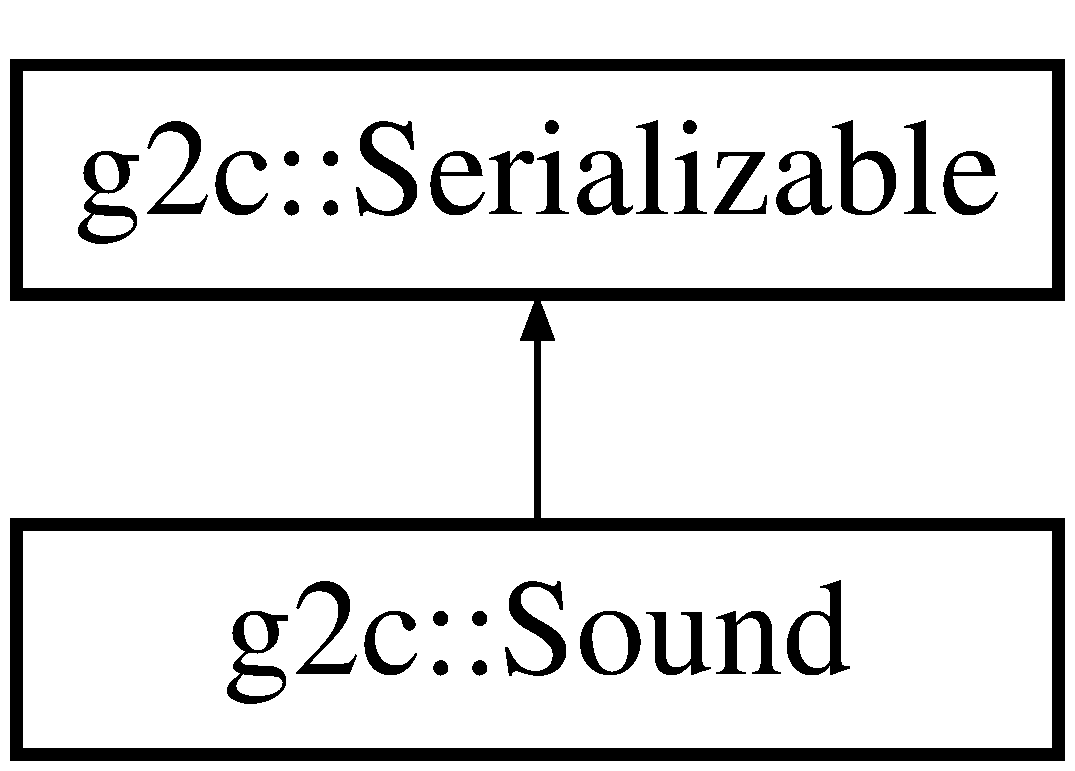
\includegraphics[height=2cm]{classg2c_1_1_sound}
\end{center}
\end{figure}
\subsection*{Public Member Functions}
\begin{DoxyCompactItemize}
\item 
\hypertarget{classg2c_1_1_sound_a607c0efbc3faf4391a68c6b3d1b3afa7}{
void {\bfseries initWithWave} (const \hyperlink{class_wave}{Wave} \&wave)}
\label{classg2c_1_1_sound_a607c0efbc3faf4391a68c6b3d1b3afa7}

\item 
\hypertarget{classg2c_1_1_sound_a79f2c2b68df5e2ff7d89a34a198650d8}{
void {\bfseries play} (double gain=1.0) const }
\label{classg2c_1_1_sound_a79f2c2b68df5e2ff7d89a34a198650d8}

\item 
\hypertarget{classg2c_1_1_sound_a4b5bdbd88913c8966c56f7ff94995a93}{
void {\bfseries stop} () const }
\label{classg2c_1_1_sound_a4b5bdbd88913c8966c56f7ff94995a93}

\item 
\hypertarget{classg2c_1_1_sound_a607fcc5472783f4b4d21caf00798112a}{
virtual std::string {\bfseries serializeElements} (std::string indent=\char`\"{}\char`\"{}) const }
\label{classg2c_1_1_sound_a607fcc5472783f4b4d21caf00798112a}

\item 
\hypertarget{classg2c_1_1_sound_a96a97a1b430792e34bd546876374fcd9}{
virtual void {\bfseries handleChild} (const \hyperlink{classparse_1_1_node}{parse::Node} $\ast$n)}
\label{classg2c_1_1_sound_a96a97a1b430792e34bd546876374fcd9}

\item 
\hypertarget{classg2c_1_1_sound_aae80f5ff99ab08c5188f9233cc2855de}{
int {\bfseries getIndex} ()}
\label{classg2c_1_1_sound_aae80f5ff99ab08c5188f9233cc2855de}

\end{DoxyCompactItemize}
\subsection*{Public Attributes}
\begin{DoxyCompactItemize}
\item 
\hypertarget{classg2c_1_1_sound_af23aa2ffa02023222953da2f6f3fa67c}{
std::string {\bfseries file}}
\label{classg2c_1_1_sound_af23aa2ffa02023222953da2f6f3fa67c}

\item 
\hypertarget{classg2c_1_1_sound_ab934f09627fbfa470405cf64b3f963a8}{
\hyperlink{classg2c_1_1_source}{Source} $\ast$ {\bfseries source}}
\label{classg2c_1_1_sound_ab934f09627fbfa470405cf64b3f963a8}

\item 
\hypertarget{classg2c_1_1_sound_a275c745fd1970d2da1cf5a5facf967f0}{
bool {\bfseries loop}}
\label{classg2c_1_1_sound_a275c745fd1970d2da1cf5a5facf967f0}

\end{DoxyCompactItemize}


The documentation for this class was generated from the following files:\begin{DoxyCompactItemize}
\item 
sound.h\item 
sound.cpp\end{DoxyCompactItemize}

\hypertarget{classg2c_1_1_source}{
\section{g2c::Source Class Reference}
\label{classg2c_1_1_source}\index{g2c::Source@{g2c::Source}}
}
\subsection*{Public Member Functions}
\begin{DoxyCompactItemize}
\item 
\hypertarget{classg2c_1_1_source_a3ba33326a68c95f48255eda5e3ad02cc}{
bool {\bfseries isPlaying} () const }
\label{classg2c_1_1_source_a3ba33326a68c95f48255eda5e3ad02cc}

\end{DoxyCompactItemize}
\subsection*{Friends}
\begin{DoxyCompactItemize}
\item 
\hypertarget{classg2c_1_1_source_a50914f77c7cf4fb97616c898c5291f4b}{
class {\bfseries Sound}}
\label{classg2c_1_1_source_a50914f77c7cf4fb97616c898c5291f4b}

\end{DoxyCompactItemize}


The documentation for this class was generated from the following files:\begin{DoxyCompactItemize}
\item 
sound.h\item 
sound.cpp\end{DoxyCompactItemize}

\hypertarget{classg2c_1_1_sprite}{
\section{g2c::Sprite Class Reference}
\label{classg2c_1_1_sprite}\index{g2c::Sprite@{g2c::Sprite}}
}


{\ttfamily \#include $<$sprites.h$>$}Inheritance diagram for g2c::Sprite::\begin{figure}[H]
\begin{center}
\leavevmode
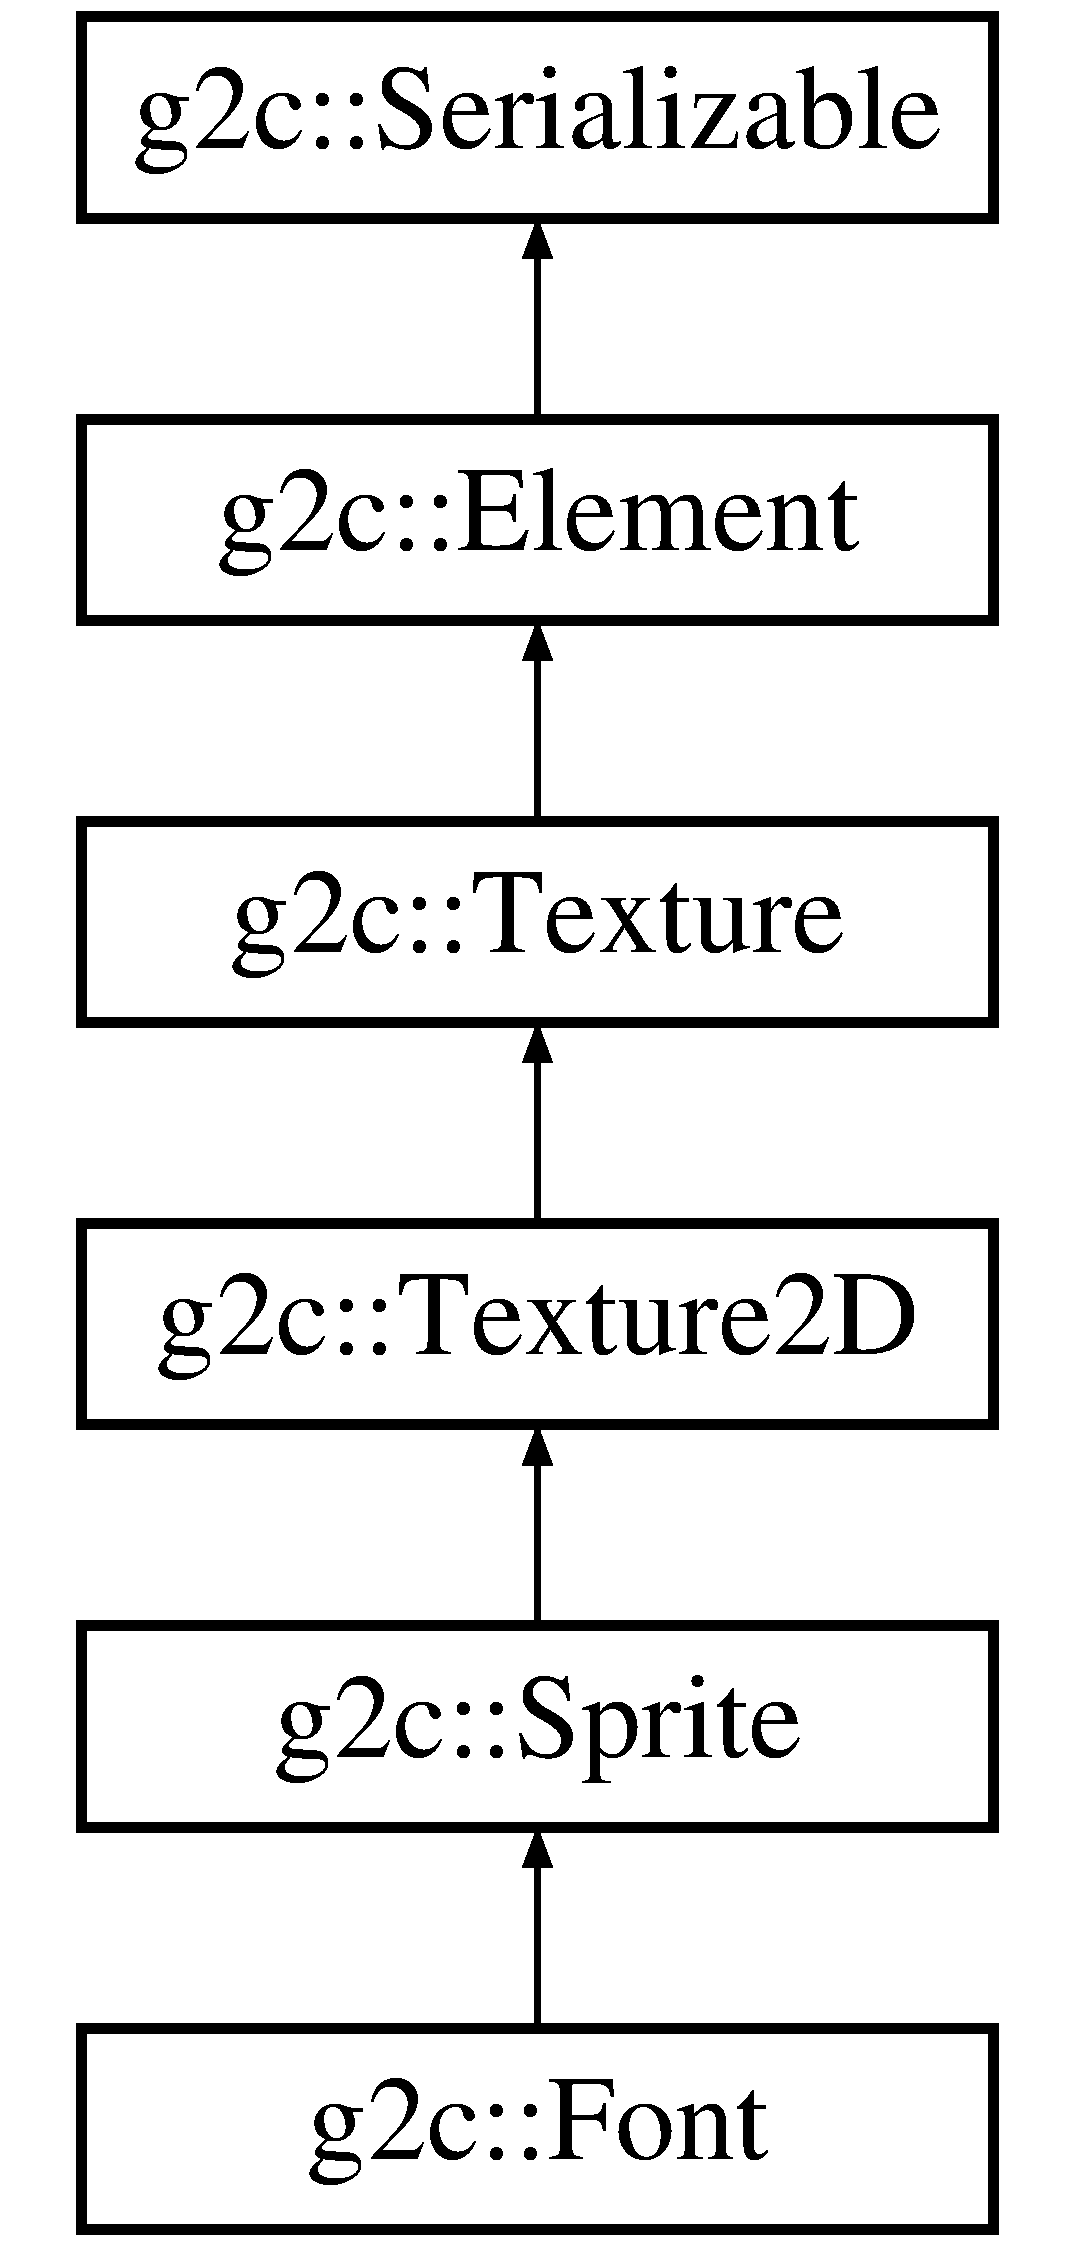
\includegraphics[height=6cm]{classg2c_1_1_sprite}
\end{center}
\end{figure}
\subsection*{Public Member Functions}
\begin{DoxyCompactItemize}
\item 
\hypertarget{classg2c_1_1_sprite_ab605111518df32637cbb10f442071a5b}{
Mat4 {\bfseries getOffsetMatrix} (double x=0.0, double y=0.0, double k=1.0) const }
\label{classg2c_1_1_sprite_ab605111518df32637cbb10f442071a5b}

\item 
\hypertarget{classg2c_1_1_sprite_a138759194d8d7be86e27dea0c6a0897b}{
Mat3 {\bfseries getTexMatrix} (int frame=0) const }
\label{classg2c_1_1_sprite_a138759194d8d7be86e27dea0c6a0897b}

\end{DoxyCompactItemize}
\subsection*{Public Attributes}
\begin{DoxyCompactItemize}
\item 
\hypertarget{classg2c_1_1_sprite_a16c5ad30837942d0687d54a04953bc94}{
\hyperlink{classg2c_1_1_string_property}{StringProperty} {\bfseries file}}
\label{classg2c_1_1_sprite_a16c5ad30837942d0687d54a04953bc94}

\item 
\hypertarget{classg2c_1_1_sprite_a950069d33a7ae543f31a596569c0a839}{
\hyperlink{classg2c_1_1_int_property}{IntProperty} {\bfseries numberOfColumns}}
\label{classg2c_1_1_sprite_a950069d33a7ae543f31a596569c0a839}

\item 
\hypertarget{classg2c_1_1_sprite_a2eea2ddb6eff64c44d4d86567103e046}{
\hyperlink{classg2c_1_1_int_property}{IntProperty} {\bfseries numberOfRows}}
\label{classg2c_1_1_sprite_a2eea2ddb6eff64c44d4d86567103e046}

\item 
\hypertarget{classg2c_1_1_sprite_a5ecdb4a09f9abbc0ca6db3c90472ae72}{
\hyperlink{classg2c_1_1_bool_property}{BoolProperty} {\bfseries center}}
\label{classg2c_1_1_sprite_a5ecdb4a09f9abbc0ca6db3c90472ae72}

\item 
\hypertarget{classg2c_1_1_sprite_a16e246843e6eab65e442dac687534780}{
\hyperlink{classg2c_1_1_bool_property}{BoolProperty} {\bfseries flipRows}}
\label{classg2c_1_1_sprite_a16e246843e6eab65e442dac687534780}

\item 
\hypertarget{classg2c_1_1_sprite_ad46d6a4c78d395f282c97e988ef51ac3}{
\hyperlink{classg2c_1_1_polygon}{Polygon} {\bfseries polygon}}
\label{classg2c_1_1_sprite_ad46d6a4c78d395f282c97e988ef51ac3}

\end{DoxyCompactItemize}
\subsection*{Static Public Attributes}
\begin{DoxyCompactItemize}
\item 
\hypertarget{classg2c_1_1_sprite_a6c1f9f057d8e505ca6f66a71343ff6a9}{
static bool {\bfseries drawLines} = false}
\label{classg2c_1_1_sprite_a6c1f9f057d8e505ca6f66a71343ff6a9}

\item 
\hypertarget{classg2c_1_1_sprite_abf2fcf0bb64c335b0a41f21fe82b5e05}{
static \hyperlink{classg2c_1_1_renderer}{Renderer} $\ast$ {\bfseries renderer} = NULL}
\label{classg2c_1_1_sprite_abf2fcf0bb64c335b0a41f21fe82b5e05}

\end{DoxyCompactItemize}
\subsection*{Protected Member Functions}
\begin{DoxyCompactItemize}
\item 
\hypertarget{classg2c_1_1_sprite_a31e0617f286d70f61664218767e7a963}{
virtual std::string {\bfseries serializeElements} (std::string indent=\char`\"{}\char`\"{}) const }
\label{classg2c_1_1_sprite_a31e0617f286d70f61664218767e7a963}

\item 
\hypertarget{classg2c_1_1_sprite_ae53a67afb41347fd05de1688b9a005f5}{
virtual void {\bfseries handleChild} (const \hyperlink{classparse_1_1_node}{parse::Node} $\ast$n)}
\label{classg2c_1_1_sprite_ae53a67afb41347fd05de1688b9a005f5}

\end{DoxyCompactItemize}


\subsection{Detailed Description}
A \hyperlink{classg2c_1_1_sprite}{Sprite} represnts a texture on the GPU whose image is a rectangular array of animation frames. For instance a chracter in a side-\/scroller could use a \hyperlink{classg2c_1_1_sprite}{Sprite} to hold all the possible poses.

\hyperlink{classg2c_1_1_sprite}{Sprite} can be initialized by using the functions of its parent class \hyperlink{classg2c_1_1_texture2_d}{Texture2D} to load in a \hyperlink{classg2c_1_1_bitmap}{Bitmap} and then setting numberOfRows and numberOfColumns.

The class \hyperlink{classg2c_1_1_actor}{Actor} is made to draw a \hyperlink{classg2c_1_1_sprite}{Sprite} on the screen with specific coordinates and current animation frames. 

The documentation for this class was generated from the following files:\begin{DoxyCompactItemize}
\item 
sprites.h\item 
sprites.cpp\end{DoxyCompactItemize}

\hypertarget{classg2c_1_1_stop_events}{
\section{g2c::StopEvents Class Reference}
\label{classg2c_1_1_stop_events}\index{g2c::StopEvents@{g2c::StopEvents}}
}
Inheritance diagram for g2c::StopEvents::\begin{figure}[H]
\begin{center}
\leavevmode
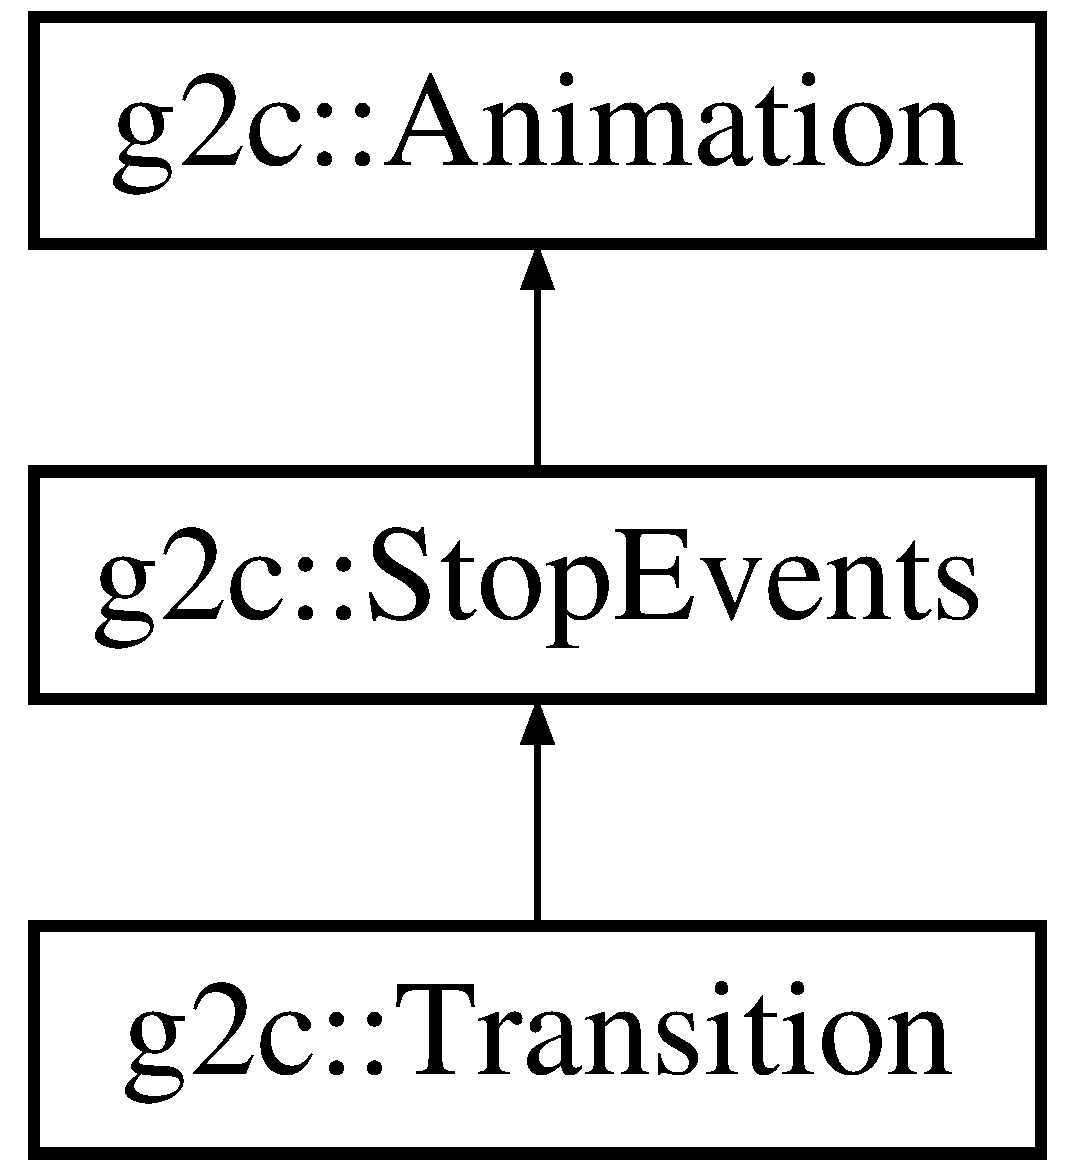
\includegraphics[height=3cm]{classg2c_1_1_stop_events}
\end{center}
\end{figure}
\subsection*{Public Member Functions}
\begin{DoxyCompactItemize}
\item 
\hypertarget{classg2c_1_1_stop_events_a371e14fed65cfe6e2451722b43451e5c}{
{\bfseries StopEvents} (double instart, double induration)}
\label{classg2c_1_1_stop_events_a371e14fed65cfe6e2451722b43451e5c}

\item 
\hypertarget{classg2c_1_1_stop_events_addfa8729eef29fba678692329d4bbfac}{
virtual void {\bfseries begin} ()}
\label{classg2c_1_1_stop_events_addfa8729eef29fba678692329d4bbfac}

\item 
\hypertarget{classg2c_1_1_stop_events_a045bcb0ad3f36ec93db2dc85167bb44e}{
virtual void {\bfseries step} (double t)}
\label{classg2c_1_1_stop_events_a045bcb0ad3f36ec93db2dc85167bb44e}

\item 
\hypertarget{classg2c_1_1_stop_events_a7fc7657d0c4679b84a6d811580014fa4}{
virtual void {\bfseries end} ()}
\label{classg2c_1_1_stop_events_a7fc7657d0c4679b84a6d811580014fa4}

\end{DoxyCompactItemize}


The documentation for this class was generated from the following files:\begin{DoxyCompactItemize}
\item 
animations.h\item 
animations.cpp\end{DoxyCompactItemize}

\hypertarget{classg2c_1_1_string_property}{
\section{g2c::StringProperty Class Reference}
\label{classg2c_1_1_string_property}\index{g2c::StringProperty@{g2c::StringProperty}}
}
Inheritance diagram for g2c::StringProperty::\begin{figure}[H]
\begin{center}
\leavevmode
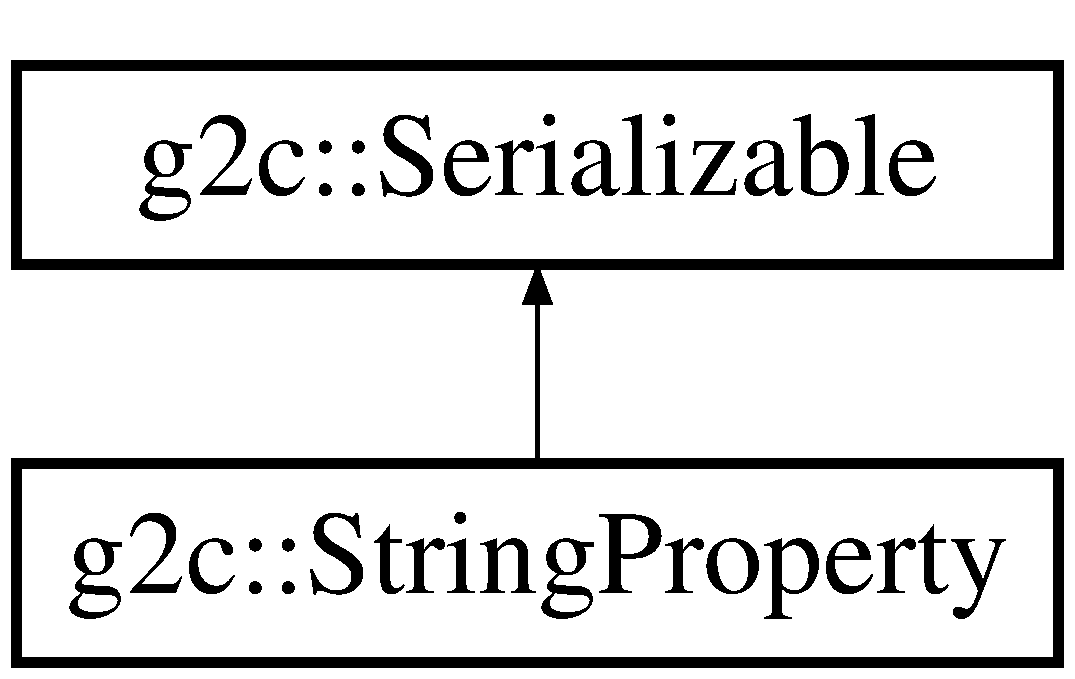
\includegraphics[height=2cm]{classg2c_1_1_string_property}
\end{center}
\end{figure}
\subsection*{Public Member Functions}
\begin{DoxyCompactItemize}
\item 
\hypertarget{classg2c_1_1_string_property_a3bf29c22a3a1f633bc466a8f51810394}{
{\bfseries StringProperty} (const std::string \&s)}
\label{classg2c_1_1_string_property_a3bf29c22a3a1f633bc466a8f51810394}

\item 
\hypertarget{classg2c_1_1_string_property_ac468096772e95ee6cf73c72dc70aadaf}{
{\bfseries StringProperty} (const char $\ast$s)}
\label{classg2c_1_1_string_property_ac468096772e95ee6cf73c72dc70aadaf}

\item 
\hypertarget{classg2c_1_1_string_property_add89345e7f914ccc0a97e80d0c413c72}{
virtual std::string {\bfseries serialize} (std::string indent=\char`\"{}\char`\"{}) const }
\label{classg2c_1_1_string_property_add89345e7f914ccc0a97e80d0c413c72}

\item 
\hypertarget{classg2c_1_1_string_property_aeed9b53e388cdf13d38d7e3d751d5e19}{
virtual void {\bfseries initWithParseNode} (const \hyperlink{classparse_1_1_node}{parse::Node} $\ast$n)}
\label{classg2c_1_1_string_property_aeed9b53e388cdf13d38d7e3d751d5e19}

\item 
\hypertarget{classg2c_1_1_string_property_a570bb8391443ae0a89ee44dbeaa80375}{
const std::string \& {\bfseries operator()} () const }
\label{classg2c_1_1_string_property_a570bb8391443ae0a89ee44dbeaa80375}

\item 
\hypertarget{classg2c_1_1_string_property_a3aebadcdea74130b156886a0a368a7a9}{
void {\bfseries operator()} (const std::string \&s)}
\label{classg2c_1_1_string_property_a3aebadcdea74130b156886a0a368a7a9}

\end{DoxyCompactItemize}


The documentation for this class was generated from the following files:\begin{DoxyCompactItemize}
\item 
serializable.h\item 
serializable.cpp\end{DoxyCompactItemize}

\hypertarget{classg2c_1_1_text}{
\section{g2c::Text Class Reference}
\label{classg2c_1_1_text}\index{g2c::Text@{g2c::Text}}
}


{\ttfamily \#include $<$sprites.h$>$}Inheritance diagram for g2c::Text::\begin{figure}[H]
\begin{center}
\leavevmode
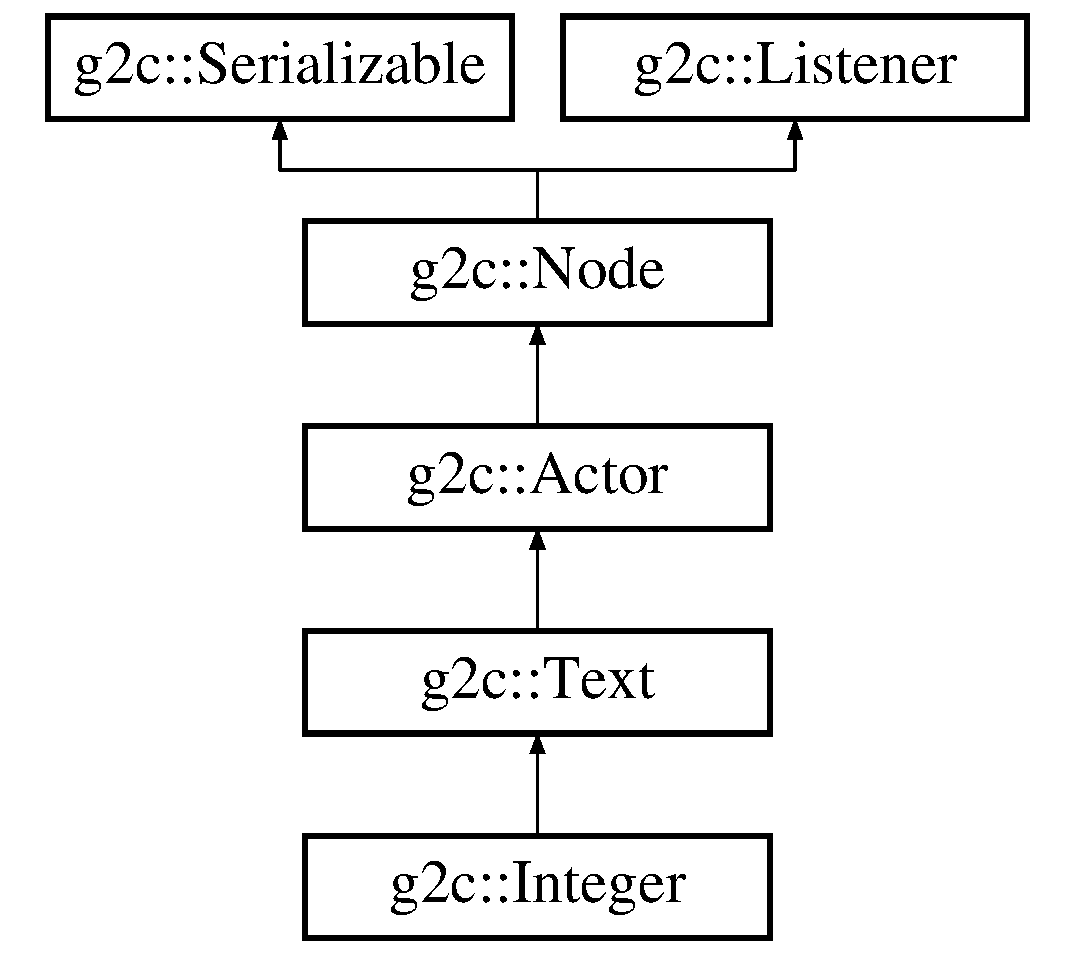
\includegraphics[height=5cm]{classg2c_1_1_text}
\end{center}
\end{figure}
\subsection*{Public Member Functions}
\begin{DoxyCompactItemize}
\item 
\hypertarget{classg2c_1_1_text_a58370a00a8812fe81985cd69bc25c163}{
{\bfseries Text} (\hyperlink{classg2c_1_1_font}{Font} $\ast$infont)}
\label{classg2c_1_1_text_a58370a00a8812fe81985cd69bc25c163}

\item 
virtual void \hyperlink{classg2c_1_1_text_ab3296a30652c4c3157ae8a8e87449bb4}{draw} () const 
\item 
\hypertarget{classg2c_1_1_text_a707929240f4ecc9113345c8128b2a749}{
virtual std::string {\bfseries serializeElements} (std::string indent) const }
\label{classg2c_1_1_text_a707929240f4ecc9113345c8128b2a749}

\item 
\hypertarget{classg2c_1_1_text_abd97b62c5a137c4410673fa8f798202f}{
virtual void {\bfseries handleChild} (const \hyperlink{classparse_1_1_node}{parse::Node} $\ast$n)}
\label{classg2c_1_1_text_abd97b62c5a137c4410673fa8f798202f}

\item 
\hypertarget{classg2c_1_1_text_a8a68d2f6ac6251a5ba158f3d7dbf0e2e}{
virtual \hyperlink{classg2c_1_1_polygon}{Polygon} {\bfseries collisionPolygon} () const }
\label{classg2c_1_1_text_a8a68d2f6ac6251a5ba158f3d7dbf0e2e}

\item 
\hypertarget{classg2c_1_1_text_ac78497d459bbece12e7a3bbd2fb877f5}{
void {\bfseries keyboard} (unsigned char inkey)}
\label{classg2c_1_1_text_ac78497d459bbece12e7a3bbd2fb877f5}

\end{DoxyCompactItemize}
\subsection*{Public Attributes}
\begin{DoxyCompactItemize}
\item 
std::string \hyperlink{classg2c_1_1_text_a0b1d9a8876fced2290eeda161d992084}{justification}
\item 
std::string \hyperlink{classg2c_1_1_text_a9b4447b44f0831b3f40ef12ebac60dc1}{s}
\item 
\hyperlink{classg2c_1_1_font}{Font} $\ast$ \hyperlink{classg2c_1_1_text_a1bb9fa51e3d58a6561d4449495d3ce75}{font}
\item 
\hypertarget{classg2c_1_1_text_a5bca37a540e7ad2d8b5f2b940473c9ac}{
std::string {\bfseries fontName}}
\label{classg2c_1_1_text_a5bca37a540e7ad2d8b5f2b940473c9ac}

\item 
\hypertarget{classg2c_1_1_text_ae352a66b9303fb1a742ce39c06a8c063}{
bool {\bfseries drawPipe}}
\label{classg2c_1_1_text_ae352a66b9303fb1a742ce39c06a8c063}

\end{DoxyCompactItemize}


\subsection{Detailed Description}
\hyperlink{classg2c_1_1_actor}{Actor} for drawing text from a string and a \hyperlink{classg2c_1_1_font}{Font} object. \hyperlink{classg2c_1_1_text_ab3296a30652c4c3157ae8a8e87449bb4}{Text::draw} draws a quad for each character in its member string s, sampling the texture represented by font to get characters. 

\subsection{Member Function Documentation}
\hypertarget{classg2c_1_1_text_ab3296a30652c4c3157ae8a8e87449bb4}{
\index{g2c::Text@{g2c::Text}!draw@{draw}}
\index{draw@{draw}!g2c::Text@{g2c::Text}}
\subsubsection[{draw}]{\setlength{\rightskip}{0pt plus 5cm}void g2c::Text::draw () const\hspace{0.3cm}{\ttfamily  \mbox{[}virtual\mbox{]}}}}
\label{classg2c_1_1_text_ab3296a30652c4c3157ae8a8e87449bb4}
Draws an image of the c++ string s using the characters in font. 

Reimplemented from \hyperlink{classg2c_1_1_actor_a587aff8d8df73dbba0c659459e094074}{g2c::Actor}.

Reimplemented in \hyperlink{classg2c_1_1_integer_aac99d7502a55bf5db01f5d673779e36e}{g2c::Integer}.

\subsection{Member Data Documentation}
\hypertarget{classg2c_1_1_text_a1bb9fa51e3d58a6561d4449495d3ce75}{
\index{g2c::Text@{g2c::Text}!font@{font}}
\index{font@{font}!g2c::Text@{g2c::Text}}
\subsubsection[{font}]{\setlength{\rightskip}{0pt plus 5cm}{\bf Font}$\ast$ {\bf g2c::Text::font}}}
\label{classg2c_1_1_text_a1bb9fa51e3d58a6561d4449495d3ce75}
A font object is a \hyperlink{classg2c_1_1_sprite}{Sprite} whose frames correspond to the characters to be drawn. \hypertarget{classg2c_1_1_text_a0b1d9a8876fced2290eeda161d992084}{
\index{g2c::Text@{g2c::Text}!justification@{justification}}
\index{justification@{justification}!g2c::Text@{g2c::Text}}
\subsubsection[{justification}]{\setlength{\rightskip}{0pt plus 5cm}std::string {\bf g2c::Text::justification}}}
\label{classg2c_1_1_text_a0b1d9a8876fced2290eeda161d992084}
A string either \char`\"{}left\char`\"{}, \char`\"{}right\char`\"{} or \char`\"{}center\char`\"{} describing how the drawn string eminates from the coordinates of this \hyperlink{classg2c_1_1_actor}{Actor}. \hypertarget{classg2c_1_1_text_a9b4447b44f0831b3f40ef12ebac60dc1}{
\index{g2c::Text@{g2c::Text}!s@{s}}
\index{s@{s}!g2c::Text@{g2c::Text}}
\subsubsection[{s}]{\setlength{\rightskip}{0pt plus 5cm}std::string {\bf g2c::Text::s}}}
\label{classg2c_1_1_text_a9b4447b44f0831b3f40ef12ebac60dc1}
A standard c++ string, this is the text that gets drawn. 

The documentation for this class was generated from the following files:\begin{DoxyCompactItemize}
\item 
sprites.h\item 
sprites.cpp\end{DoxyCompactItemize}

\hypertarget{classg2c_1_1_texture}{
\section{g2c::Texture Class Reference}
\label{classg2c_1_1_texture}\index{g2c::Texture@{g2c::Texture}}
}
Inheritance diagram for g2c::Texture::\begin{figure}[H]
\begin{center}
\leavevmode
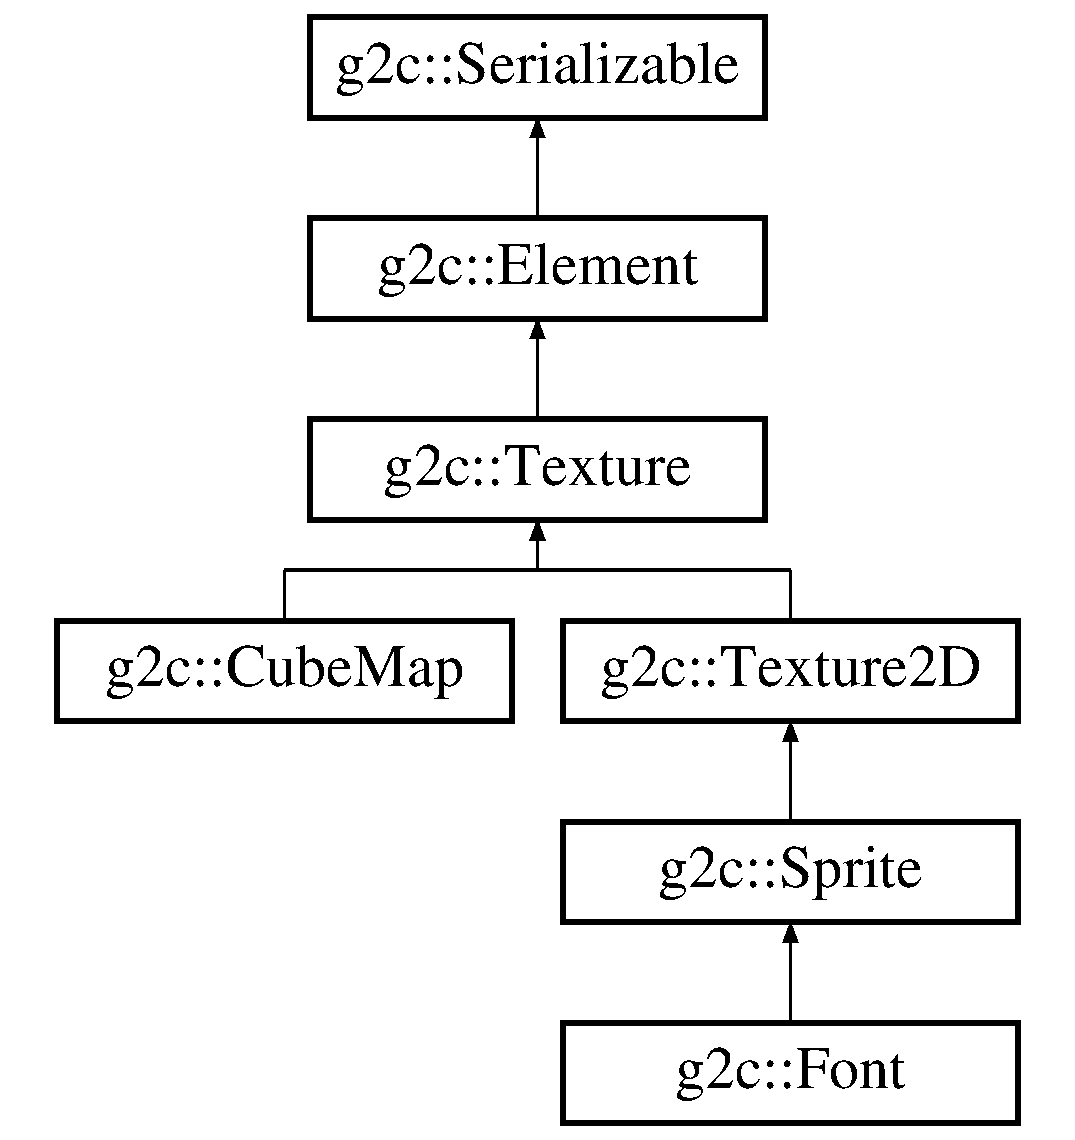
\includegraphics[height=6cm]{classg2c_1_1_texture}
\end{center}
\end{figure}
\subsection*{Public Member Functions}
\begin{DoxyCompactItemize}
\item 
\hypertarget{classg2c_1_1_texture_adc2d0f45ef1e489e04abd84ddd7c8439}{
GLuint {\bfseries getUnit} () const }
\label{classg2c_1_1_texture_adc2d0f45ef1e489e04abd84ddd7c8439}

\item 
\hypertarget{classg2c_1_1_texture_a63c9b6f6119976d505cc0a0750256460}{
GLuint {\bfseries getIndex} () const }
\label{classg2c_1_1_texture_a63c9b6f6119976d505cc0a0750256460}

\item 
\hypertarget{classg2c_1_1_texture_ab9caf8729da624fa63df9959fc0e06f0}{
GLuint {\bfseries getTarget} () const }
\label{classg2c_1_1_texture_ab9caf8729da624fa63df9959fc0e06f0}

\item 
\hypertarget{classg2c_1_1_texture_a53cddf5c787468975e52730f33e777e1}{
virtual std::string {\bfseries serializeElements} (std::string indent=\char`\"{}\char`\"{}) const }
\label{classg2c_1_1_texture_a53cddf5c787468975e52730f33e777e1}

\item 
\hypertarget{classg2c_1_1_texture_a8e9fe06fa6fbf8b55989cc0ea447e938}{
virtual void {\bfseries handleChild} (const \hyperlink{classparse_1_1_node}{parse::Node} $\ast$n)}
\label{classg2c_1_1_texture_a8e9fe06fa6fbf8b55989cc0ea447e938}

\end{DoxyCompactItemize}
\subsection*{Public Attributes}
\begin{DoxyCompactItemize}
\item 
\hypertarget{classg2c_1_1_texture_a2b89faead5e4f502145ec5956761e584}{
int {\bfseries bitsPerPixel}}
\label{classg2c_1_1_texture_a2b89faead5e4f502145ec5956761e584}

\item 
\hypertarget{classg2c_1_1_texture_adaa9e5c89ebb48ff7b7a8c1fdef7cf47}{
GLuint {\bfseries index}}
\label{classg2c_1_1_texture_adaa9e5c89ebb48ff7b7a8c1fdef7cf47}

\item 
\hypertarget{classg2c_1_1_texture_a6856a6c3123e7e460d42d5271b972075}{
GLuint {\bfseries unit}}
\label{classg2c_1_1_texture_a6856a6c3123e7e460d42d5271b972075}

\item 
\hypertarget{classg2c_1_1_texture_aeb86198c4a40480939cc1f9301358b00}{
GLenum {\bfseries target}}
\label{classg2c_1_1_texture_aeb86198c4a40480939cc1f9301358b00}

\end{DoxyCompactItemize}
\subsection*{Protected Member Functions}
\begin{DoxyCompactItemize}
\item 
\hypertarget{classg2c_1_1_texture_ab23136f9906ebf166ddb24e7f4f0f33d}{
{\bfseries Texture} (GLenum target)}
\label{classg2c_1_1_texture_ab23136f9906ebf166ddb24e7f4f0f33d}

\item 
\hypertarget{classg2c_1_1_texture_a29144eec65a861ffd1b5bc338702d3d2}{
{\bfseries Texture} (GLenum target, int unit)}
\label{classg2c_1_1_texture_a29144eec65a861ffd1b5bc338702d3d2}

\end{DoxyCompactItemize}
\subsection*{Protected Attributes}
\begin{DoxyCompactItemize}
\item 
\hypertarget{classg2c_1_1_texture_a9db4665866938aeb9b5cec76371ef4ac}{
bool {\bfseries mipmaps}}
\label{classg2c_1_1_texture_a9db4665866938aeb9b5cec76371ef4ac}

\end{DoxyCompactItemize}


The documentation for this class was generated from the following files:\begin{DoxyCompactItemize}
\item 
texture.h\item 
texture.cpp\end{DoxyCompactItemize}

\hypertarget{classg2c_1_1_texture2_d}{
\section{g2c::Texture2D Class Reference}
\label{classg2c_1_1_texture2_d}\index{g2c::Texture2D@{g2c::Texture2D}}
}
Inheritance diagram for g2c::Texture2D::\begin{figure}[H]
\begin{center}
\leavevmode
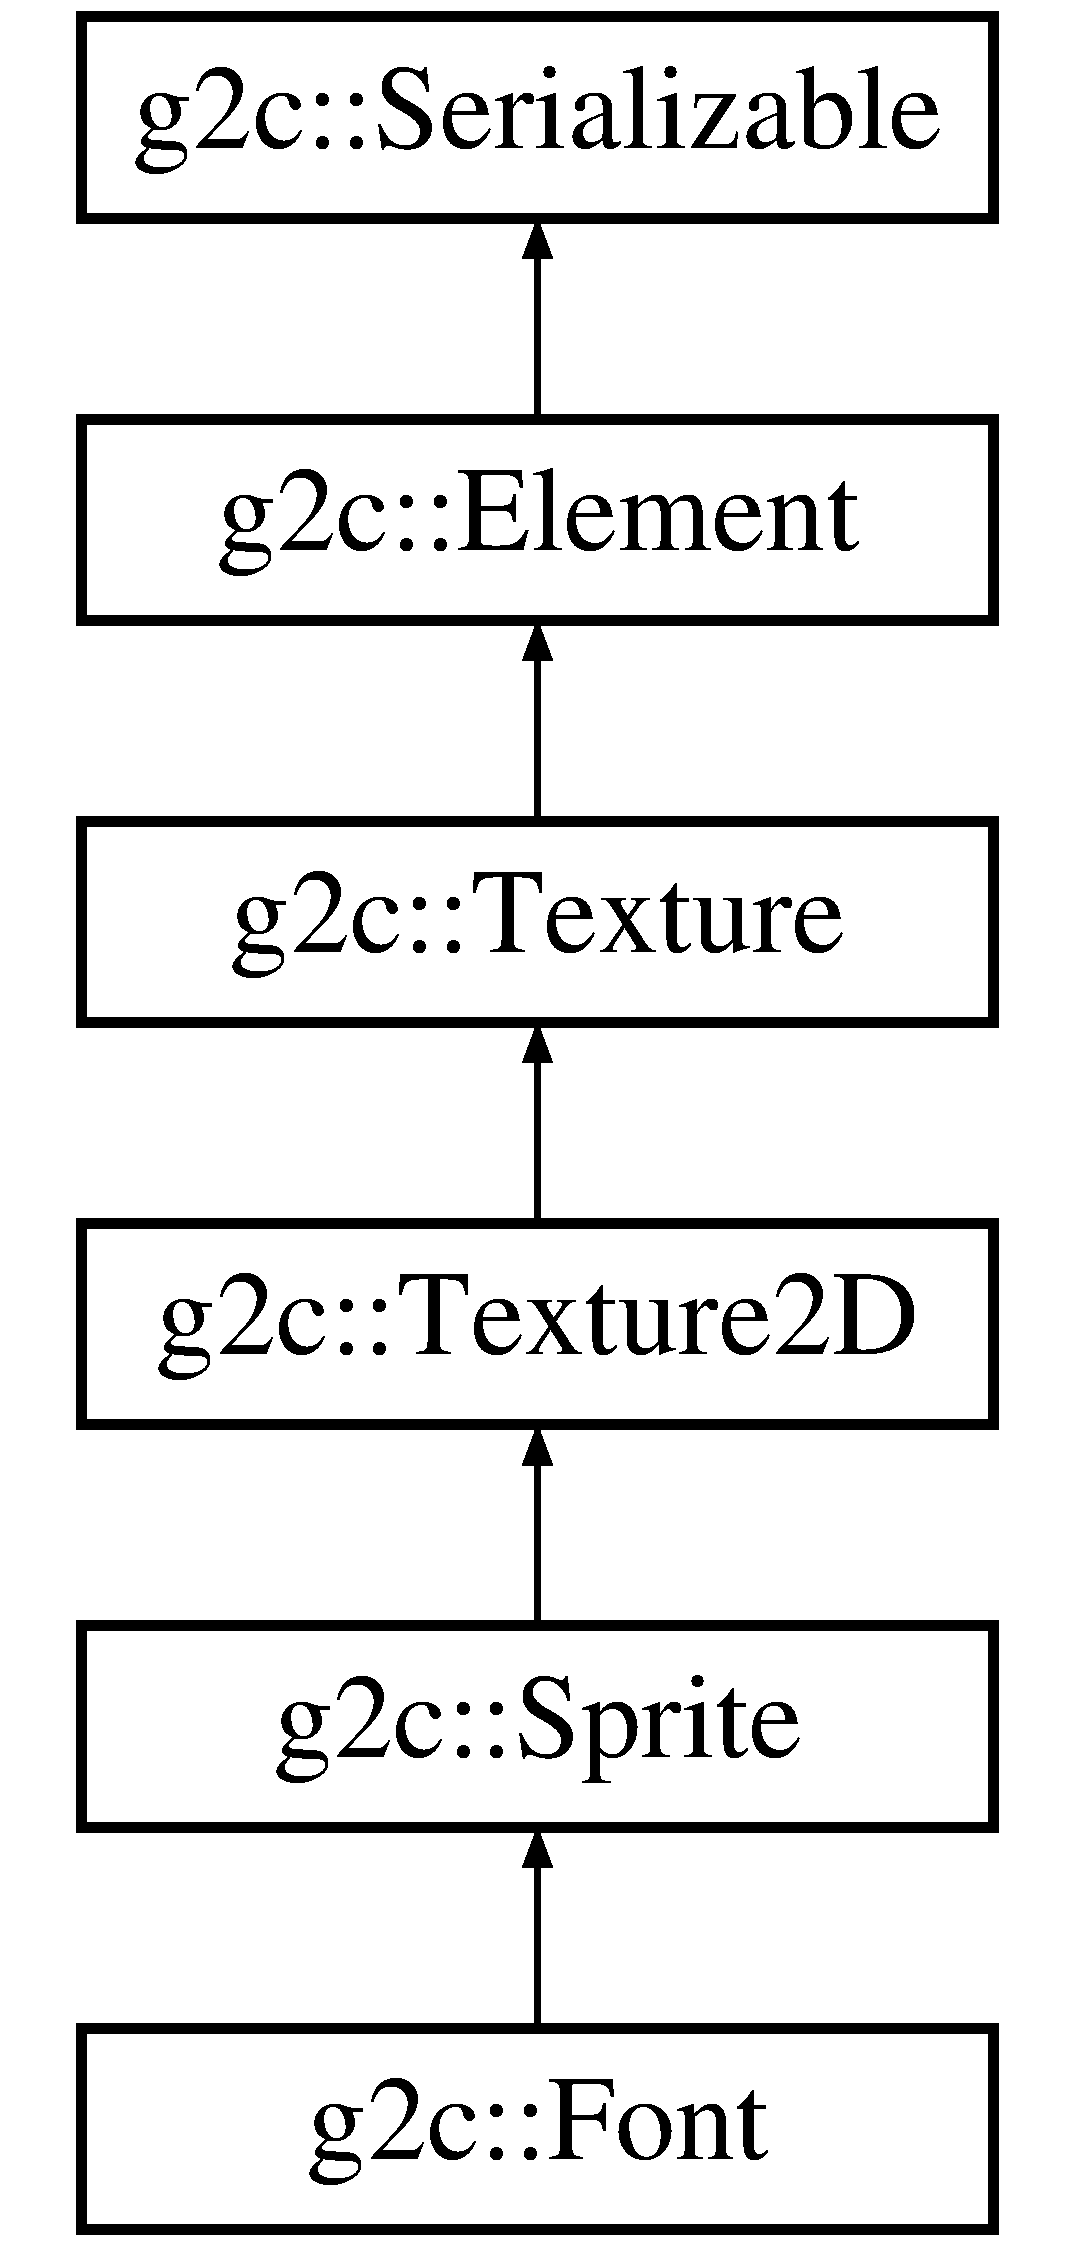
\includegraphics[height=6cm]{classg2c_1_1_texture2_d}
\end{center}
\end{figure}
\subsection*{Public Member Functions}
\begin{DoxyCompactItemize}
\item 
\hypertarget{classg2c_1_1_texture2_d_ad29455116e90b411faf6d113bd9dfb3f}{
{\bfseries Texture2D} (int unit)}
\label{classg2c_1_1_texture2_d_ad29455116e90b411faf6d113bd9dfb3f}

\item 
\hypertarget{classg2c_1_1_texture2_d_a9d59a7f32d06a8335624929d607ae18e}{
void {\bfseries initWithImageData} (const GLubyte $\ast$inData, int inWidth, int inHeight, int inBitsPerPixel)}
\label{classg2c_1_1_texture2_d_a9d59a7f32d06a8335624929d607ae18e}

\item 
\hypertarget{classg2c_1_1_texture2_d_ab194586c1ed8e48f9acdc67878569fb7}{
void {\bfseries initWithBitmap} (const \hyperlink{classg2c_1_1_bitmap}{Bitmap} \&bitmap)}
\label{classg2c_1_1_texture2_d_ab194586c1ed8e48f9acdc67878569fb7}

\item 
\hypertarget{classg2c_1_1_texture2_d_a2622ef69a99eb593810332cecd78f74b}{
virtual std::string {\bfseries serializeElements} (std::string indent=\char`\"{}\char`\"{}) const }
\label{classg2c_1_1_texture2_d_a2622ef69a99eb593810332cecd78f74b}

\item 
\hypertarget{classg2c_1_1_texture2_d_a9b1bcddd36df970855242c98057f9de5}{
virtual void {\bfseries handleChild} (const \hyperlink{classparse_1_1_node}{parse::Node} $\ast$n)}
\label{classg2c_1_1_texture2_d_a9b1bcddd36df970855242c98057f9de5}

\end{DoxyCompactItemize}
\subsection*{Public Attributes}
\begin{DoxyCompactItemize}
\item 
\hypertarget{classg2c_1_1_texture2_d_ae0054c114f58b881bac49ae26a3e5c36}{
GLubyte $\ast$ {\bfseries data}}
\label{classg2c_1_1_texture2_d_ae0054c114f58b881bac49ae26a3e5c36}

\item 
\hypertarget{classg2c_1_1_texture2_d_a1055a22a350fbc3affcec5092068b4a7}{
int {\bfseries width}}
\label{classg2c_1_1_texture2_d_a1055a22a350fbc3affcec5092068b4a7}

\item 
\hypertarget{classg2c_1_1_texture2_d_a8a36ceb7d62906800782a0adf7aa2f61}{
int {\bfseries height}}
\label{classg2c_1_1_texture2_d_a8a36ceb7d62906800782a0adf7aa2f61}

\item 
\hypertarget{classg2c_1_1_texture2_d_a6ae225bcd225ef67d6fc2d7d7ac0697e}{
std::string {\bfseries file}}
\label{classg2c_1_1_texture2_d_a6ae225bcd225ef67d6fc2d7d7ac0697e}

\end{DoxyCompactItemize}
\subsection*{Friends}
\begin{DoxyCompactItemize}
\item 
\hypertarget{classg2c_1_1_texture2_d_aeceedf6e1a7d48a588516ce2b1983d6f}{
class {\bfseries Value}}
\label{classg2c_1_1_texture2_d_aeceedf6e1a7d48a588516ce2b1983d6f}

\end{DoxyCompactItemize}


The documentation for this class was generated from the following files:\begin{DoxyCompactItemize}
\item 
texture.h\item 
texture.cpp\end{DoxyCompactItemize}

\hypertarget{classg2c_1_1_transition}{
\section{g2c::Transition Class Reference}
\label{classg2c_1_1_transition}\index{g2c::Transition@{g2c::Transition}}
}
Inheritance diagram for g2c::Transition::\begin{figure}[H]
\begin{center}
\leavevmode
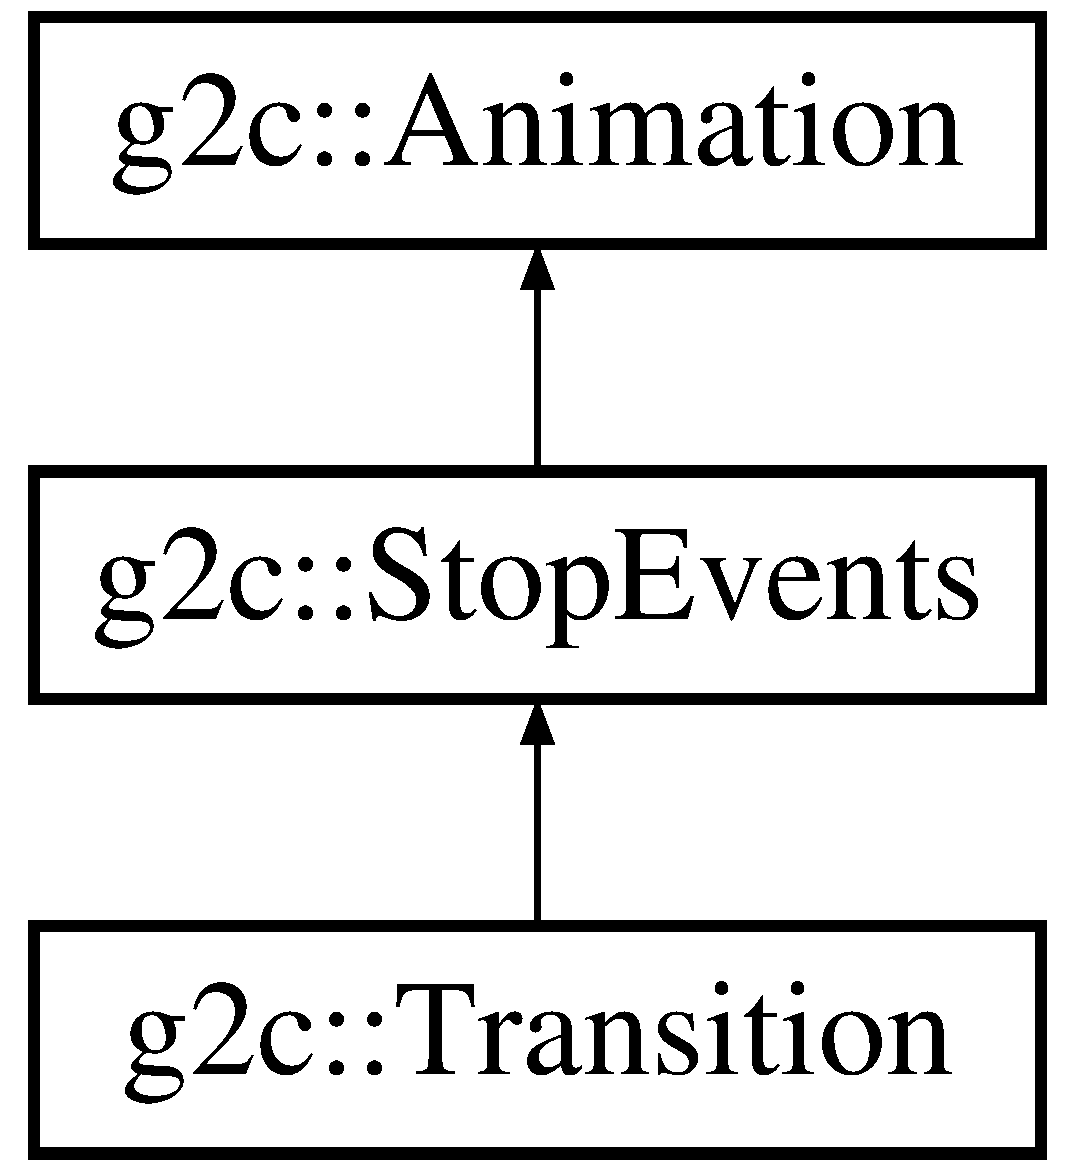
\includegraphics[height=3cm]{classg2c_1_1_transition}
\end{center}
\end{figure}
\subsection*{Public Member Functions}
\begin{DoxyCompactItemize}
\item 
\hypertarget{classg2c_1_1_transition_a236ef3a3da46070e0a3fedae0ece734d}{
{\bfseries Transition} (double instart, double induration, \hyperlink{classg2c_1_1_node}{Node} $\ast$outgoing, \hyperlink{classg2c_1_1_node}{Node} $\ast$incoming)}
\label{classg2c_1_1_transition_a236ef3a3da46070e0a3fedae0ece734d}

\item 
\hypertarget{classg2c_1_1_transition_a9d38f69d1a050e6f1ea46dcf1b3ca80e}{
virtual void {\bfseries begin} ()}
\label{classg2c_1_1_transition_a9d38f69d1a050e6f1ea46dcf1b3ca80e}

\item 
\hypertarget{classg2c_1_1_transition_a2f79705527b0c91591732c829488c7d8}{
virtual void {\bfseries step} (double t)}
\label{classg2c_1_1_transition_a2f79705527b0c91591732c829488c7d8}

\item 
\hypertarget{classg2c_1_1_transition_aacc901d902e303815859bd04b72be737}{
virtual void {\bfseries end} ()}
\label{classg2c_1_1_transition_aacc901d902e303815859bd04b72be737}

\end{DoxyCompactItemize}
\subsection*{Public Attributes}
\begin{DoxyCompactItemize}
\item 
\hypertarget{classg2c_1_1_transition_a18fc15af3ff46f351799186abe263a70}{
\hyperlink{classg2c_1_1_node}{Node} $\ast$ {\bfseries outgoing}}
\label{classg2c_1_1_transition_a18fc15af3ff46f351799186abe263a70}

\item 
\hypertarget{classg2c_1_1_transition_aae574b923cdbb5a6d969ea79d74dee56}{
\hyperlink{classg2c_1_1_node}{Node} $\ast$ {\bfseries incoming}}
\label{classg2c_1_1_transition_aae574b923cdbb5a6d969ea79d74dee56}

\end{DoxyCompactItemize}


The documentation for this class was generated from the following files:\begin{DoxyCompactItemize}
\item 
animations.h\item 
animations.cpp\end{DoxyCompactItemize}

\hypertarget{classg2c_1_1_value}{
\section{g2c::Value Class Reference}
\label{classg2c_1_1_value}\index{g2c::Value@{g2c::Value}}
}
\subsection*{Classes}
\begin{DoxyCompactItemize}
\item 
union {\bfseries Data}
\end{DoxyCompactItemize}
\subsection*{Public Types}
\begin{DoxyCompactItemize}
\item 
enum {\bfseries Type} \{ \par
{\bfseries NONE}, 
{\bfseries FLOAT}, 
{\bfseries VEC2}, 
{\bfseries VEC3}, 
\par
{\bfseries VEC4}, 
{\bfseries MAT2}, 
{\bfseries MAT3}, 
{\bfseries MAT4}, 
\par
{\bfseries TEXTURE}
 \}
\end{DoxyCompactItemize}
\subsection*{Public Member Functions}
\begin{DoxyCompactItemize}
\item 
\hypertarget{classg2c_1_1_value_a214a6284cbc21ceb3f33c77d9d3095e1}{
{\bfseries Value} (const \hyperlink{classg2c_1_1_value}{Value} \&v)}
\label{classg2c_1_1_value_a214a6284cbc21ceb3f33c77d9d3095e1}

\item 
\hypertarget{classg2c_1_1_value_a27f95e137ee2aa52896e1ba5946d9eda}{
{\bfseries Value} (float t)}
\label{classg2c_1_1_value_a27f95e137ee2aa52896e1ba5946d9eda}

\item 
\hypertarget{classg2c_1_1_value_a71aa35765d370234bccae9dd535b049d}{
{\bfseries Value} (const Vec2 \&t)}
\label{classg2c_1_1_value_a71aa35765d370234bccae9dd535b049d}

\item 
\hypertarget{classg2c_1_1_value_a4ab8d3d53ed7a56ef9ec88a4aba6b137}{
{\bfseries Value} (const Vec3 \&t)}
\label{classg2c_1_1_value_a4ab8d3d53ed7a56ef9ec88a4aba6b137}

\item 
\hypertarget{classg2c_1_1_value_adc7821a3348e7404daca36662847e9ab}{
{\bfseries Value} (const Vec4 \&t)}
\label{classg2c_1_1_value_adc7821a3348e7404daca36662847e9ab}

\item 
\hypertarget{classg2c_1_1_value_abf509dd8d7ea90cb650d9f00c5ca1a65}{
{\bfseries Value} (const Mat2 \&t)}
\label{classg2c_1_1_value_abf509dd8d7ea90cb650d9f00c5ca1a65}

\item 
\hypertarget{classg2c_1_1_value_ae4d30b1924bfd45b10ce820e50882193}{
{\bfseries Value} (const Mat3 \&t)}
\label{classg2c_1_1_value_ae4d30b1924bfd45b10ce820e50882193}

\item 
\hypertarget{classg2c_1_1_value_a635331bc68f3e58a7f63f25285087d3b}{
{\bfseries Value} (const Mat4 \&t)}
\label{classg2c_1_1_value_a635331bc68f3e58a7f63f25285087d3b}

\item 
\hypertarget{classg2c_1_1_value_ac91de4e0a0e3c7bb832a03ff59a6e9a6}{
{\bfseries Value} (const \hyperlink{classg2c_1_1_texture}{Texture} $\ast$t)}
\label{classg2c_1_1_value_ac91de4e0a0e3c7bb832a03ff59a6e9a6}

\item 
\hypertarget{classg2c_1_1_value_affb4cff78b519667994ae075cce2be1e}{
\hyperlink{classg2c_1_1_value}{Value} \& {\bfseries operator=} (const \hyperlink{classg2c_1_1_value}{Value} \&v)}
\label{classg2c_1_1_value_affb4cff78b519667994ae075cce2be1e}

\item 
\hypertarget{classg2c_1_1_value_af8cdb1c197e22bfc84be9525538747e6}{
float {\bfseries getFloat} () const }
\label{classg2c_1_1_value_af8cdb1c197e22bfc84be9525538747e6}

\item 
\hypertarget{classg2c_1_1_value_ac0f42a35725e5831e34440135aa5e806}{
Vec2 {\bfseries getVec2} () const }
\label{classg2c_1_1_value_ac0f42a35725e5831e34440135aa5e806}

\item 
\hypertarget{classg2c_1_1_value_ad184ef70572f68b2594b9925bfbcb56d}{
Vec3 {\bfseries getVec3} () const }
\label{classg2c_1_1_value_ad184ef70572f68b2594b9925bfbcb56d}

\item 
\hypertarget{classg2c_1_1_value_a81fd98e6c48e9c247f694d2549705d14}{
Vec4 {\bfseries getVec4} () const }
\label{classg2c_1_1_value_a81fd98e6c48e9c247f694d2549705d14}

\item 
\hypertarget{classg2c_1_1_value_ad9f2144e1c86c60e88e19001d0e5d556}{
Mat2 {\bfseries getMat2} () const }
\label{classg2c_1_1_value_ad9f2144e1c86c60e88e19001d0e5d556}

\item 
\hypertarget{classg2c_1_1_value_aab3706833fa8337b686e4611ac782ef3}{
Mat3 {\bfseries getMat3} () const }
\label{classg2c_1_1_value_aab3706833fa8337b686e4611ac782ef3}

\item 
\hypertarget{classg2c_1_1_value_a7dd34c269bec21b6e3cae81528e3e275}{
Mat4 {\bfseries getMat4} () const }
\label{classg2c_1_1_value_a7dd34c269bec21b6e3cae81528e3e275}

\item 
\hypertarget{classg2c_1_1_value_a746aef948675640db3046bf7b6223a44}{
const \hyperlink{classg2c_1_1_texture}{Texture} $\ast$ {\bfseries getTexture} () const }
\label{classg2c_1_1_value_a746aef948675640db3046bf7b6223a44}

\item 
\hypertarget{classg2c_1_1_value_a05a75dafa6753fa8de22c0503e84a456}{
void {\bfseries applyToLocation} (GLuint location) const }
\label{classg2c_1_1_value_a05a75dafa6753fa8de22c0503e84a456}

\item 
\hypertarget{classg2c_1_1_value_ab7d2b67ccddb584f27e22d928d809b76}{
std::string {\bfseries toString} () const }
\label{classg2c_1_1_value_ab7d2b67ccddb584f27e22d928d809b76}

\end{DoxyCompactItemize}
\subsection*{Public Attributes}
\begin{DoxyCompactItemize}
\item 
\hypertarget{classg2c_1_1_value_adf86b70809fc12705dacbd7b8cdcfb73}{
enum g2c::Value::Type {\bfseries type}}
\label{classg2c_1_1_value_adf86b70809fc12705dacbd7b8cdcfb73}

\item 
\hypertarget{classg2c_1_1_value_ab847b4a4e1d11a628192ec1c1246500e}{
std::string {\bfseries textureName}}
\label{classg2c_1_1_value_ab847b4a4e1d11a628192ec1c1246500e}

\end{DoxyCompactItemize}


The documentation for this class was generated from the following files:\begin{DoxyCompactItemize}
\item 
graphics.h\item 
graphics.cpp\end{DoxyCompactItemize}

\hypertarget{classg2c_1_1_vec2_property}{
\section{g2c::Vec2Property Class Reference}
\label{classg2c_1_1_vec2_property}\index{g2c::Vec2Property@{g2c::Vec2Property}}
}
Inheritance diagram for g2c::Vec2Property::\begin{figure}[H]
\begin{center}
\leavevmode
\includegraphics[height=2cm]{classg2c_1_1_vec2_property}
\end{center}
\end{figure}
\subsection*{Public Member Functions}
\begin{DoxyCompactItemize}
\item 
\hypertarget{classg2c_1_1_vec2_property_af9deb0e1b63b3da4cc626b5143d84706}{
{\bfseries Vec2Property} (const Vec2 \&v)}
\label{classg2c_1_1_vec2_property_af9deb0e1b63b3da4cc626b5143d84706}

\item 
\hypertarget{classg2c_1_1_vec2_property_ade5f28ec67ffc3503769666812ba43e0}{
virtual std::string {\bfseries serialize} (std::string indent) const }
\label{classg2c_1_1_vec2_property_ade5f28ec67ffc3503769666812ba43e0}

\item 
\hypertarget{classg2c_1_1_vec2_property_a7b767b039d126a1029ebb60438618e8f}{
void {\bfseries initWithParseNode} (const \hyperlink{classparse_1_1_node}{parse::Node} $\ast$n)}
\label{classg2c_1_1_vec2_property_a7b767b039d126a1029ebb60438618e8f}

\end{DoxyCompactItemize}


The documentation for this class was generated from the following files:\begin{DoxyCompactItemize}
\item 
sprites.h\item 
sprites.cpp\end{DoxyCompactItemize}

\hypertarget{classg2c_1_1_vec3_property}{
\section{g2c::Vec3Property Class Reference}
\label{classg2c_1_1_vec3_property}\index{g2c::Vec3Property@{g2c::Vec3Property}}
}
Inheritance diagram for g2c::Vec3Property::\begin{figure}[H]
\begin{center}
\leavevmode
\includegraphics[height=2cm]{classg2c_1_1_vec3_property}
\end{center}
\end{figure}
\subsection*{Public Member Functions}
\begin{DoxyCompactItemize}
\item 
\hypertarget{classg2c_1_1_vec3_property_ab2add6037ab51695b7d739b59bd08917}{
{\bfseries Vec3Property} (const Vec3 \&v)}
\label{classg2c_1_1_vec3_property_ab2add6037ab51695b7d739b59bd08917}

\item 
\hypertarget{classg2c_1_1_vec3_property_ab1e805ec02b9d9f69ba0b2847acb7458}{
virtual std::string {\bfseries serialize} (std::string indent) const }
\label{classg2c_1_1_vec3_property_ab1e805ec02b9d9f69ba0b2847acb7458}

\item 
\hypertarget{classg2c_1_1_vec3_property_ac4725a2803b95da44c0a2dae712036eb}{
void {\bfseries initWithParseNode} (const \hyperlink{classparse_1_1_node}{parse::Node} $\ast$n)}
\label{classg2c_1_1_vec3_property_ac4725a2803b95da44c0a2dae712036eb}

\end{DoxyCompactItemize}


The documentation for this class was generated from the following files:\begin{DoxyCompactItemize}
\item 
sprites.h\item 
sprites.cpp\end{DoxyCompactItemize}

\hypertarget{classstd_1_1vector}{
\section{vector Class Reference}
\label{classstd_1_1vector}\index{std::vector@{std::vector}}
}


Inherited by \hyperlink{classg2c_1_1_pointer_vector_property}{g2c::PointerVectorProperty$<$ Node $\ast$ $>$}, \hyperlink{classg2c_1_1_pointer_vector_property}{g2c::PointerVectorProperty$<$ Sound $\ast$ $>$}, \hyperlink{classg2c_1_1_pointer_vector_property}{g2c::PointerVectorProperty$<$ Sprite $\ast$ $>$}, and \hyperlink{classg2c_1_1_vector_property}{g2c::VectorProperty$<$ Vec2Property $>$}.

The documentation for this class was generated from the following file:\begin{DoxyCompactItemize}
\item 
serializable.h\end{DoxyCompactItemize}

\hypertarget{classg2c_1_1_vector_property}{
\section{g2c::VectorProperty$<$ T $>$ Class Template Reference}
\label{classg2c_1_1_vector_property}\index{g2c::VectorProperty@{g2c::VectorProperty}}
}
Inheritance diagram for g2c::VectorProperty$<$ T $>$::\begin{figure}[H]
\begin{center}
\leavevmode
\includegraphics[height=2cm]{classg2c_1_1_vector_property}
\end{center}
\end{figure}
\subsection*{Public Member Functions}
\begin{DoxyCompactItemize}
\item 
\hypertarget{classg2c_1_1_vector_property_a50ced1da338478b66b1384acc5486313}{
{\bfseries VectorProperty} (const std::vector$<$ T $>$ \&v)}
\label{classg2c_1_1_vector_property_a50ced1da338478b66b1384acc5486313}

\item 
\hypertarget{classg2c_1_1_vector_property_ae76d578bde928b7684fb3bc822f5fd98}{
virtual std::string {\bfseries serialize} (std::string indent=\char`\"{}\char`\"{}) const }
\label{classg2c_1_1_vector_property_ae76d578bde928b7684fb3bc822f5fd98}

\item 
\hypertarget{classg2c_1_1_vector_property_a826e44f19343e6fc96f54f3b3d364cd0}{
void {\bfseries initWithParseNode} (const \hyperlink{classparse_1_1_node}{parse::Node} $\ast$n)}
\label{classg2c_1_1_vector_property_a826e44f19343e6fc96f54f3b3d364cd0}

\end{DoxyCompactItemize}
\subsubsection*{template$<$class T$>$ class g2c::VectorProperty$<$ T $>$}



The documentation for this class was generated from the following file:\begin{DoxyCompactItemize}
\item 
serializable.h\end{DoxyCompactItemize}

\hypertarget{classg2c_1_1_walk_int}{
\section{g2c::WalkInt Class Reference}
\label{classg2c_1_1_walk_int}\index{g2c::WalkInt@{g2c::WalkInt}}
}
Inheritance diagram for g2c::WalkInt::\begin{figure}[H]
\begin{center}
\leavevmode
\includegraphics[height=2cm]{classg2c_1_1_walk_int}
\end{center}
\end{figure}
\subsection*{Public Member Functions}
\begin{DoxyCompactItemize}
\item 
\hypertarget{classg2c_1_1_walk_int_a094ba0dcf6f6e0fbe849f59f64379cbb}{
{\bfseries WalkInt} (double instart, double induration, int $\ast$ina, int infirst, int inlast)}
\label{classg2c_1_1_walk_int_a094ba0dcf6f6e0fbe849f59f64379cbb}

\item 
\hypertarget{classg2c_1_1_walk_int_a56d4d9d4d0234992cfc408b07902798f}{
virtual void {\bfseries begin} ()}
\label{classg2c_1_1_walk_int_a56d4d9d4d0234992cfc408b07902798f}

\item 
\hypertarget{classg2c_1_1_walk_int_ac0a60bb999ab2ceac8f335de46d28277}{
virtual void {\bfseries step} (double t)}
\label{classg2c_1_1_walk_int_ac0a60bb999ab2ceac8f335de46d28277}

\item 
\hypertarget{classg2c_1_1_walk_int_afedba0ea401f0889a63df7118f1485ce}{
virtual void {\bfseries end} ()}
\label{classg2c_1_1_walk_int_afedba0ea401f0889a63df7118f1485ce}

\end{DoxyCompactItemize}
\subsection*{Public Attributes}
\begin{DoxyCompactItemize}
\item 
\hypertarget{classg2c_1_1_walk_int_a8d11535301461dd83cfab7567781258a}{
int $\ast$ {\bfseries a}}
\label{classg2c_1_1_walk_int_a8d11535301461dd83cfab7567781258a}

\item 
\hypertarget{classg2c_1_1_walk_int_ad1564a81f5776f0e9b84f8e269881be8}{
int {\bfseries first}}
\label{classg2c_1_1_walk_int_ad1564a81f5776f0e9b84f8e269881be8}

\item 
\hypertarget{classg2c_1_1_walk_int_acce15f6d2ea333cb30f9691dd987cdb5}{
int {\bfseries last}}
\label{classg2c_1_1_walk_int_acce15f6d2ea333cb30f9691dd987cdb5}

\end{DoxyCompactItemize}


The documentation for this class was generated from the following files:\begin{DoxyCompactItemize}
\item 
animations.h\item 
animations.cpp\end{DoxyCompactItemize}

\hypertarget{class_wave}{
\section{Wave Class Reference}
\label{class_wave}\index{Wave@{Wave}}
}
\subsection*{Public Member Functions}
\begin{DoxyCompactItemize}
\item 
\hypertarget{class_wave_a33db4a869b15584198d36c80f6bee284}{
void {\bfseries initWithData} (const uint8\_\-t $\ast$data, size\_\-t size)}
\label{class_wave_a33db4a869b15584198d36c80f6bee284}

\end{DoxyCompactItemize}
\subsection*{Public Attributes}
\begin{DoxyCompactItemize}
\item 
\hypertarget{class_wave_ad4b9f9e4844087071f221b44d69baf41}{
int {\bfseries sampleRate}}
\label{class_wave_ad4b9f9e4844087071f221b44d69baf41}

\item 
\hypertarget{class_wave_a19c7abafddb96a810fb370a7a0e8914b}{
int {\bfseries numChannels}}
\label{class_wave_a19c7abafddb96a810fb370a7a0e8914b}

\item 
\hypertarget{class_wave_a03caf3727c678e29026bd3628468aaa7}{
int {\bfseries numSamples}}
\label{class_wave_a03caf3727c678e29026bd3628468aaa7}

\item 
\hypertarget{class_wave_a3e60209058fd253011ce449245c813a1}{
int {\bfseries bytesPerSample}}
\label{class_wave_a3e60209058fd253011ce449245c813a1}

\item 
\hypertarget{class_wave_a626e52590fd144f7054109b1ce256db0}{
uint8\_\-t $\ast$ {\bfseries data}}
\label{class_wave_a626e52590fd144f7054109b1ce256db0}

\end{DoxyCompactItemize}


The documentation for this class was generated from the following files:\begin{DoxyCompactItemize}
\item 
wave.h\item 
wave.cpp\end{DoxyCompactItemize}

\hypertarget{struct_wav_header}{
\section{WavHeader Struct Reference}
\label{struct_wav_header}\index{WavHeader@{WavHeader}}
}
\subsection*{Public Attributes}
\begin{DoxyCompactItemize}
\item 
\hypertarget{struct_wav_header_ad12ee1a19f7bb81ad702d6abb8e61d85}{
char {\bfseries waveTag} \mbox{[}4\mbox{]}}
\label{struct_wav_header_ad12ee1a19f7bb81ad702d6abb8e61d85}

\item 
\hypertarget{struct_wav_header_a28b241e83f636464281cd4d2b246f280}{
char {\bfseries fmtTag} \mbox{[}4\mbox{]}}
\label{struct_wav_header_a28b241e83f636464281cd4d2b246f280}

\item 
\hypertarget{struct_wav_header_a986d76d500914f370cddfa6c2f1542d2}{
int {\bfseries Subchunk1Size}}
\label{struct_wav_header_a986d76d500914f370cddfa6c2f1542d2}

\item 
\hypertarget{struct_wav_header_af052ba52da4a1bda137ce0171f3d763e}{
short {\bfseries audioFormat}}
\label{struct_wav_header_af052ba52da4a1bda137ce0171f3d763e}

\item 
\hypertarget{struct_wav_header_a974f24ee8f6c0f7a6a881b1b5f917bfa}{
short {\bfseries numChannels}}
\label{struct_wav_header_a974f24ee8f6c0f7a6a881b1b5f917bfa}

\item 
\hypertarget{struct_wav_header_a70f6545b7646e8f9c2f02118150566d1}{
int {\bfseries sampleRate}}
\label{struct_wav_header_a70f6545b7646e8f9c2f02118150566d1}

\item 
\hypertarget{struct_wav_header_ab9c193dd57da1a877cd5193657ed8a75}{
int {\bfseries byteRate}}
\label{struct_wav_header_ab9c193dd57da1a877cd5193657ed8a75}

\item 
\hypertarget{struct_wav_header_a1bfbf825695b7626f58e64355a3ee4b1}{
short {\bfseries blockAlign}}
\label{struct_wav_header_a1bfbf825695b7626f58e64355a3ee4b1}

\item 
\hypertarget{struct_wav_header_a2dbf27f9cd07e02e744d4f71bc25109b}{
short {\bfseries bitsPerSample}}
\label{struct_wav_header_a2dbf27f9cd07e02e744d4f71bc25109b}

\item 
\hypertarget{struct_wav_header_a7f07365285e299b1014b1e3add1fc271}{
char {\bfseries dataTag} \mbox{[}4\mbox{]}}
\label{struct_wav_header_a7f07365285e299b1014b1e3add1fc271}

\item 
\hypertarget{struct_wav_header_a501041ecccd8debd17d35e5d59844164}{
int {\bfseries dataSize}}
\label{struct_wav_header_a501041ecccd8debd17d35e5d59844164}

\end{DoxyCompactItemize}


The documentation for this struct was generated from the following file:\begin{DoxyCompactItemize}
\item 
wave.cpp\end{DoxyCompactItemize}

\hypertarget{classg2c_1_1_windows_bank}{
\section{g2c::WindowsBank Class Reference}
\label{classg2c_1_1_windows_bank}\index{g2c::WindowsBank@{g2c::WindowsBank}}
}
Inheritance diagram for g2c::WindowsBank::\begin{figure}[H]
\begin{center}
\leavevmode
\includegraphics[height=2cm]{classg2c_1_1_windows_bank}
\end{center}
\end{figure}
\subsection*{Public Member Functions}
\begin{DoxyCompactItemize}
\item 
\hypertarget{classg2c_1_1_windows_bank_a8df2b4df3248d565aca7a85b1db6e8b2}{
virtual void {\bfseries initPersistentSerializableWithKey} (\hyperlink{classg2c_1_1_serializable}{Serializable} $\ast$s, const char $\ast$key)}
\label{classg2c_1_1_windows_bank_a8df2b4df3248d565aca7a85b1db6e8b2}

\item 
\hypertarget{classg2c_1_1_windows_bank_afb4f651b3529237c2b7554d79ee46520}{
virtual void {\bfseries writePersistentSerializableWithKey} (const \hyperlink{classg2c_1_1_serializable}{Serializable} $\ast$s, const char $\ast$key)}
\label{classg2c_1_1_windows_bank_afb4f651b3529237c2b7554d79ee46520}

\item 
\hypertarget{classg2c_1_1_windows_bank_a661ea280d1eff46c9333a22d8e259028}{
virtual void {\bfseries initSerializableWithPath} (\hyperlink{classg2c_1_1_serializable}{Serializable} $\ast$s, const char $\ast$path)}
\label{classg2c_1_1_windows_bank_a661ea280d1eff46c9333a22d8e259028}

\item 
\hypertarget{classg2c_1_1_windows_bank_a2f2ab74b7a01a0433a0d90028564ab59}{
virtual void {\bfseries writeSerializableToPath} (const \hyperlink{classg2c_1_1_serializable}{Serializable} $\ast$s, const char $\ast$path)}
\label{classg2c_1_1_windows_bank_a2f2ab74b7a01a0433a0d90028564ab59}

\item 
\hypertarget{classg2c_1_1_windows_bank_a51a30d90ab58c056005cede7cdc98ef2}{
virtual void {\bfseries initTextureWithPath} (\hyperlink{classg2c_1_1_texture2_d}{Texture2D} $\ast$texture, const char $\ast$path)}
\label{classg2c_1_1_windows_bank_a51a30d90ab58c056005cede7cdc98ef2}

\item 
\hypertarget{classg2c_1_1_windows_bank_a82f2c88f73ec24b205724cb38509f441}{
virtual void {\bfseries initBitmapWithPath} (\hyperlink{classg2c_1_1_bitmap}{Bitmap} $\ast$bitmap, const char $\ast$path)}
\label{classg2c_1_1_windows_bank_a82f2c88f73ec24b205724cb38509f441}

\item 
\hypertarget{classg2c_1_1_windows_bank_a8fb161bf739a0593ef94f1a41a297a6a}{
virtual void {\bfseries initSoundWithPath} (\hyperlink{classg2c_1_1_sound}{Sound} $\ast$sound, const char $\ast$path)}
\label{classg2c_1_1_windows_bank_a8fb161bf739a0593ef94f1a41a297a6a}

\item 
\hypertarget{classg2c_1_1_windows_bank_a3b8741751dfb82375030266ff6bd347f}{
void $\ast$ {\bfseries getOpenALAudioData} (CFURLRef inFileURL, ALsizei $\ast$outDataSize, ALenum $\ast$outDataFormat, ALsizei $\ast$outSampleRate) const }
\label{classg2c_1_1_windows_bank_a3b8741751dfb82375030266ff6bd347f}

\end{DoxyCompactItemize}
\subsection*{Public Attributes}
\begin{DoxyCompactItemize}
\item 
\hypertarget{classg2c_1_1_windows_bank_ad377e1d8151bd0523db1e600603c3ffe}{
std::string {\bfseries base\_\-path}}
\label{classg2c_1_1_windows_bank_ad377e1d8151bd0523db1e600603c3ffe}

\end{DoxyCompactItemize}
\subsection*{Protected Attributes}
\begin{DoxyCompactItemize}
\item 
\hypertarget{classg2c_1_1_windows_bank_a326056cc86dbdd94bf9e8fd4f377390a}{
std::string {\bfseries directory}}
\label{classg2c_1_1_windows_bank_a326056cc86dbdd94bf9e8fd4f377390a}

\end{DoxyCompactItemize}


The documentation for this class was generated from the following files:\begin{DoxyCompactItemize}
\item 
windowsbank.h\item 
windowsbank.cpp\end{DoxyCompactItemize}

\hypertarget{classg2c_1_1_world}{
\section{g2c::World Class Reference}
\label{classg2c_1_1_world}\index{g2c::World@{g2c::World}}
}
Inheritance diagram for g2c::World::\begin{figure}[H]
\begin{center}
\leavevmode
\includegraphics[height=3cm]{classg2c_1_1_world}
\end{center}
\end{figure}
\subsection*{Public Member Functions}
\begin{DoxyCompactItemize}
\item 
\hypertarget{classg2c_1_1_world_a89ea53bb9b6d3707cf2c0b7962bfa737}{
virtual void {\bfseries draw} () const }
\label{classg2c_1_1_world_a89ea53bb9b6d3707cf2c0b7962bfa737}

\item 
\hypertarget{classg2c_1_1_world_a6831ffc6d36c02ba3d7483bafed27024}{
virtual void {\bfseries resize} (int width, int height)}
\label{classg2c_1_1_world_a6831ffc6d36c02ba3d7483bafed27024}

\item 
\hypertarget{classg2c_1_1_world_af463addaa10be8b1ca3950950ca2f6ca}{
void {\bfseries addSprite} (\hyperlink{classg2c_1_1_sprite}{Sprite} $\ast$sprite)}
\label{classg2c_1_1_world_af463addaa10be8b1ca3950950ca2f6ca}

\item 
\hypertarget{classg2c_1_1_world_ad7fa162a6b1f464a8fb3762053d53353}{
virtual void {\bfseries removeSprite} (const \hyperlink{classg2c_1_1_sprite}{Sprite} $\ast$sprite)}
\label{classg2c_1_1_world_ad7fa162a6b1f464a8fb3762053d53353}

\item 
\hypertarget{classg2c_1_1_world_a885f5b4302faa8ee1330852d5b3ee35c}{
void {\bfseries clear} ()}
\label{classg2c_1_1_world_a885f5b4302faa8ee1330852d5b3ee35c}

\item 
\hypertarget{classg2c_1_1_world_a8b089f07c3bc3850fcb2f7cfd3bfda53}{
virtual void {\bfseries keyboard} (unsigned char inkey)}
\label{classg2c_1_1_world_a8b089f07c3bc3850fcb2f7cfd3bfda53}

\item 
\hypertarget{classg2c_1_1_world_a49e7c3d3d1b3a5047d1ecf3e24cf8687}{
virtual bool {\bfseries mouseDown} (const Vec2 \&C)}
\label{classg2c_1_1_world_a49e7c3d3d1b3a5047d1ecf3e24cf8687}

\item 
\hypertarget{classg2c_1_1_world_a125b1536baaf56642d664e211ce62b36}{
virtual void {\bfseries mouseDragged} (const Vec2 \&C)}
\label{classg2c_1_1_world_a125b1536baaf56642d664e211ce62b36}

\item 
\hypertarget{classg2c_1_1_world_af46d3cdc3aa030e3a7249b7068e98358}{
virtual void {\bfseries mouseUp} (const Vec2 \&C)}
\label{classg2c_1_1_world_af46d3cdc3aa030e3a7249b7068e98358}

\item 
\hypertarget{classg2c_1_1_world_abec479405f41fb409e45f2f3f95221d5}{
virtual void {\bfseries initWithPath} (const char $\ast$path)}
\label{classg2c_1_1_world_abec479405f41fb409e45f2f3f95221d5}

\item 
\hypertarget{classg2c_1_1_world_a7573e885cda4e30031b3efdf11e2e80a}{
virtual void {\bfseries initWithParseNode} (const \hyperlink{classparse_1_1_node}{parse::Node} $\ast$n)}
\label{classg2c_1_1_world_a7573e885cda4e30031b3efdf11e2e80a}

\item 
\hypertarget{classg2c_1_1_world_ab6736c233042a5075eaa7e9b3b62bc3a}{
virtual void {\bfseries handleChild} (const \hyperlink{classparse_1_1_node}{parse::Node} $\ast$n)}
\label{classg2c_1_1_world_ab6736c233042a5075eaa7e9b3b62bc3a}

\item 
\hypertarget{classg2c_1_1_world_ab4f21ff26324de94bad4b69002ed0f42}{
std::string {\bfseries serializeSprites} (std::string indent=\char`\"{}\char`\"{}) const }
\label{classg2c_1_1_world_ab4f21ff26324de94bad4b69002ed0f42}

\item 
\hypertarget{classg2c_1_1_world_accf3c96d6ce3c756a5df81d2ff207781}{
virtual void {\bfseries playSound} (const std::string \&name, double gain=1.0) const }
\label{classg2c_1_1_world_accf3c96d6ce3c756a5df81d2ff207781}

\item 
\hypertarget{classg2c_1_1_world_a76eda32d784c0cca606a19bb3765c956}{
\hyperlink{classg2c_1_1_sound}{g2c::Sound} $\ast$ {\bfseries getSound} (const std::string \&name)}
\label{classg2c_1_1_world_a76eda32d784c0cca606a19bb3765c956}

\item 
\hypertarget{classg2c_1_1_world_ad98f5d279d3aa9b8eaedef6f376703ff}{
virtual \hyperlink{classg2c_1_1_node}{Node} $\ast$ {\bfseries getNode} (const std::string \&name)}
\label{classg2c_1_1_world_ad98f5d279d3aa9b8eaedef6f376703ff}

\item 
\hypertarget{classg2c_1_1_world_ac278006c08abb3a26fe066d67029194e}{
virtual \hyperlink{classg2c_1_1_sprite}{Sprite} $\ast$ {\bfseries getSprite} (const std::string \&name)}
\label{classg2c_1_1_world_ac278006c08abb3a26fe066d67029194e}

\end{DoxyCompactItemize}
\subsection*{Public Attributes}
\begin{DoxyCompactItemize}
\item 
\hypertarget{classg2c_1_1_world_ae0214f6de363ec9a97c3ce5f3327f60e}{
\hyperlink{classg2c_1_1_bank}{Bank} $\ast$ {\bfseries bank}}
\label{classg2c_1_1_world_ae0214f6de363ec9a97c3ce5f3327f60e}

\item 
\hypertarget{classg2c_1_1_world_ab6a0f0e192b314634dc27bcfdff5bd17}{
\hyperlink{classg2c_1_1_pointer_vector_property}{PointerVectorProperty}$<$ \hyperlink{classg2c_1_1_sprite}{Sprite} $\ast$ $>$ {\bfseries sprites}}
\label{classg2c_1_1_world_ab6a0f0e192b314634dc27bcfdff5bd17}

\item 
\hypertarget{classg2c_1_1_world_ad163b3312a82df4ebe8eed50b0dbedc3}{
\hyperlink{classg2c_1_1_pointer_vector_property}{PointerVectorProperty}$<$ \hyperlink{classg2c_1_1_sound}{Sound} $\ast$ $>$ {\bfseries sounds}}
\label{classg2c_1_1_world_ad163b3312a82df4ebe8eed50b0dbedc3}

\end{DoxyCompactItemize}
\subsection*{Friends}
\begin{DoxyCompactItemize}
\item 
\hypertarget{classg2c_1_1_world_ae4af50bf1743d112cb2c2c784bea21c8}{
class {\bfseries Actor}}
\label{classg2c_1_1_world_ae4af50bf1743d112cb2c2c784bea21c8}

\end{DoxyCompactItemize}


The documentation for this class was generated from the following files:\begin{DoxyCompactItemize}
\item 
sprites.h\item 
sprites.cpp\end{DoxyCompactItemize}

\printindex
\end{document}
